\documentclass[twoside]{book}

% Packages required by doxygen
\usepackage{fixltx2e}
\usepackage{calc}
\usepackage{doxygen}
\usepackage[export]{adjustbox} % also loads graphicx
\usepackage{graphicx}
\usepackage[utf8]{inputenc}
\usepackage{makeidx}
\usepackage{multicol}
\usepackage{multirow}
\PassOptionsToPackage{warn}{textcomp}
\usepackage{textcomp}
\usepackage[nointegrals]{wasysym}
\usepackage[table]{xcolor}

% Font selection
\usepackage[T1]{fontenc}
\usepackage[scaled=.90]{helvet}
\usepackage{courier}
\usepackage{amssymb}
\usepackage{sectsty}
\renewcommand{\familydefault}{\sfdefault}
\allsectionsfont{%
  \fontseries{bc}\selectfont%
  \color{darkgray}%
}
\renewcommand{\DoxyLabelFont}{%
  \fontseries{bc}\selectfont%
  \color{darkgray}%
}
\newcommand{\+}{\discretionary{\mbox{\scriptsize$\hookleftarrow$}}{}{}}

% Page & text layout
\usepackage{geometry}
\geometry{%
  a4paper,%
  top=2.5cm,%
  bottom=2.5cm,%
  left=2.5cm,%
  right=2.5cm%
}
\tolerance=750
\hfuzz=15pt
\hbadness=750
\setlength{\emergencystretch}{15pt}
\setlength{\parindent}{0cm}
\setlength{\parskip}{3ex plus 2ex minus 2ex}
\makeatletter
\renewcommand{\paragraph}{%
  \@startsection{paragraph}{4}{0ex}{-1.0ex}{1.0ex}{%
    \normalfont\normalsize\bfseries\SS@parafont%
  }%
}
\renewcommand{\subparagraph}{%
  \@startsection{subparagraph}{5}{0ex}{-1.0ex}{1.0ex}{%
    \normalfont\normalsize\bfseries\SS@subparafont%
  }%
}
\makeatother

% Headers & footers
\usepackage{fancyhdr}
\pagestyle{fancyplain}
\fancyhead[LE]{\fancyplain{}{\bfseries\thepage}}
\fancyhead[CE]{\fancyplain{}{}}
\fancyhead[RE]{\fancyplain{}{\bfseries\leftmark}}
\fancyhead[LO]{\fancyplain{}{\bfseries\rightmark}}
\fancyhead[CO]{\fancyplain{}{}}
\fancyhead[RO]{\fancyplain{}{\bfseries\thepage}}
\fancyfoot[LE]{\fancyplain{}{}}
\fancyfoot[CE]{\fancyplain{}{}}
\fancyfoot[RE]{\fancyplain{}{\bfseries\scriptsize Generated by Doxygen }}
\fancyfoot[LO]{\fancyplain{}{\bfseries\scriptsize Generated by Doxygen }}
\fancyfoot[CO]{\fancyplain{}{}}
\fancyfoot[RO]{\fancyplain{}{}}
\renewcommand{\footrulewidth}{0.4pt}
\renewcommand{\chaptermark}[1]{%
  \markboth{#1}{}%
}
\renewcommand{\sectionmark}[1]{%
  \markright{\thesection\ #1}%
}

% Indices & bibliography
\usepackage{natbib}
\usepackage[titles]{tocloft}
\setcounter{tocdepth}{3}
\setcounter{secnumdepth}{5}
\makeindex

% Hyperlinks (required, but should be loaded last)
\usepackage{ifpdf}
\ifpdf
  \usepackage[pdftex,pagebackref=true]{hyperref}
\else
  \usepackage[ps2pdf,pagebackref=true]{hyperref}
\fi
\hypersetup{%
  colorlinks=true,%
  linkcolor=blue,%
  citecolor=blue,%
  unicode%
}

% Custom commands
\newcommand{\clearemptydoublepage}{%
  \newpage{\pagestyle{empty}\cleardoublepage}%
}

\usepackage{caption}
\captionsetup{labelsep=space,justification=centering,font={bf},singlelinecheck=off,skip=4pt,position=top}

%===== C O N T E N T S =====

\begin{document}

% Titlepage & ToC
\hypersetup{pageanchor=false,
             bookmarksnumbered=true,
             pdfencoding=unicode
            }
\pagenumbering{roman}
\begin{titlepage}
\vspace*{7cm}
\begin{center}%
{\Large U\+T\+Computer\+\_\+\+Doxygen }\\
\vspace*{1cm}
{\large Generated by Doxygen 1.8.11}\\
\end{center}
\end{titlepage}
\clearemptydoublepage
\tableofcontents
\clearemptydoublepage
\pagenumbering{arabic}
\hypersetup{pageanchor=true}

%--- Begin generated contents ---
\chapter{Hierarchical Index}
\section{Class Hierarchy}
This inheritance list is sorted roughly, but not completely, alphabetically\+:\begin{DoxyCompactList}
\item \contentsline{section}{Pile\+:\+:iterator}{\pageref{class_pile_1_1iterator}}{}
\item \contentsline{section}{Li\+Exception}{\pageref{class_li_exception}}{}
\item \contentsline{section}{Litterale}{\pageref{class_litterale}}{}
\begin{DoxyCompactList}
\item \contentsline{section}{Li\+Complexe}{\pageref{class_li_complexe}}{}
\item \contentsline{section}{Li\+Expression}{\pageref{class_li_expression}}{}
\item \contentsline{section}{Li\+Numerique}{\pageref{class_li_numerique}}{}
\begin{DoxyCompactList}
\item \contentsline{section}{Li\+Entiere}{\pageref{class_li_entiere}}{}
\item \contentsline{section}{Li\+Rationnelle}{\pageref{class_li_rationnelle}}{}
\item \contentsline{section}{Li\+Reelle}{\pageref{class_li_reelle}}{}
\end{DoxyCompactList}
\end{DoxyCompactList}
\item \contentsline{section}{Memento}{\pageref{class_memento}}{}
\item Q\+Main\+Window\begin{DoxyCompactList}
\item \contentsline{section}{Main\+Window}{\pageref{class_main_window}}{}
\end{DoxyCompactList}
\item Q\+Object\begin{DoxyCompactList}
\item \contentsline{section}{Calculatrice}{\pageref{class_calculatrice}}{}
\item \contentsline{section}{Pile}{\pageref{class_pile}}{}
\end{DoxyCompactList}
\item \contentsline{section}{The}{\pageref{class_the}}{}
\end{DoxyCompactList}

\chapter{Class Index}
\section{Class List}
Here are the classes, structs, unions and interfaces with brief descriptions\+:\begin{DoxyCompactList}
\item\contentsline{section}{\hyperlink{class_calculatrice}{Calculatrice} }{\pageref{class_calculatrice}}{}
\item\contentsline{section}{\hyperlink{class_pile_1_1iterator}{Pile\+::iterator} \\*\hyperlink{class_the}{The} iterator class }{\pageref{class_pile_1_1iterator}}{}
\item\contentsline{section}{\hyperlink{class_li_complexe}{Li\+Complexe} }{\pageref{class_li_complexe}}{}
\item\contentsline{section}{\hyperlink{class_li_entiere}{Li\+Entiere} }{\pageref{class_li_entiere}}{}
\item\contentsline{section}{\hyperlink{class_li_exception}{Li\+Exception} }{\pageref{class_li_exception}}{}
\item\contentsline{section}{\hyperlink{class_li_expression}{Li\+Expression} }{\pageref{class_li_expression}}{}
\item\contentsline{section}{\hyperlink{class_li_numerique}{Li\+Numerique} }{\pageref{class_li_numerique}}{}
\item\contentsline{section}{\hyperlink{class_li_rationnelle}{Li\+Rationnelle} }{\pageref{class_li_rationnelle}}{}
\item\contentsline{section}{\hyperlink{class_li_reelle}{Li\+Reelle} }{\pageref{class_li_reelle}}{}
\item\contentsline{section}{\hyperlink{class_litterale}{Litterale} }{\pageref{class_litterale}}{}
\item\contentsline{section}{\hyperlink{class_main_window}{Main\+Window} \\*\hyperlink{class_the}{The} \hyperlink{class_main_window}{Main\+Window} class }{\pageref{class_main_window}}{}
\item\contentsline{section}{\hyperlink{class_memento}{Memento} }{\pageref{class_memento}}{}
\item\contentsline{section}{\hyperlink{class_pile}{Pile} }{\pageref{class_pile}}{}
\item\contentsline{section}{\hyperlink{class_the}{The} \\*Class to manage the calculator }{\pageref{class_the}}{}
\end{DoxyCompactList}

\chapter{File Index}
\section{File List}
Here is a list of all documented files with brief descriptions\+:\begin{DoxyCompactList}
\item\contentsline{section}{\hyperlink{calculatrice_8cpp}{calculatrice.\+cpp} \\*File where the methods of the \hyperlink{class_calculatrice}{Calculatrice} class are defined }{\pageref{calculatrice_8cpp}}{}
\item\contentsline{section}{\hyperlink{calculatrice_8h}{calculatrice.\+h} \\*File where the class \hyperlink{class_calculatrice}{Calculatrice} is defined }{\pageref{calculatrice_8h}}{}
\item\contentsline{section}{\hyperlink{licomplexe_8cpp}{licomplexe.\+cpp} \\*File where the methods of the \hyperlink{class_li_complexe}{Li\+Complexe} class are defined }{\pageref{licomplexe_8cpp}}{}
\item\contentsline{section}{\hyperlink{licomplexe_8h}{licomplexe.\+h} \\*File where the class \hyperlink{class_li_complexe}{Li\+Complexe} is defined }{\pageref{licomplexe_8h}}{}
\item\contentsline{section}{\hyperlink{lientiere_8cpp}{lientiere.\+cpp} \\*File where the methods of the \hyperlink{class_li_entiere}{Li\+Entiere} class are defined }{\pageref{lientiere_8cpp}}{}
\item\contentsline{section}{\hyperlink{lientiere_8h}{lientiere.\+h} \\*File where the class \hyperlink{class_li_entiere}{Li\+Entiere} is defined }{\pageref{lientiere_8h}}{}
\item\contentsline{section}{\hyperlink{liexception_8h}{liexception.\+h} \\*File where the class managing the exception is defined }{\pageref{liexception_8h}}{}
\item\contentsline{section}{\hyperlink{liexpression_8cpp}{liexpression.\+cpp} \\*File where the methods of the \hyperlink{class_li_expression}{Li\+Expression} class are defined }{\pageref{liexpression_8cpp}}{}
\item\contentsline{section}{\hyperlink{liexpression_8h}{liexpression.\+h} \\*File where the class \hyperlink{class_li_expression}{Li\+Expression} is defined }{\pageref{liexpression_8h}}{}
\item\contentsline{section}{\hyperlink{linumerique_8h}{linumerique.\+h} \\*File where the class \hyperlink{class_li_numerique}{Li\+Numerique} is defined }{\pageref{linumerique_8h}}{}
\item\contentsline{section}{\hyperlink{lirationnelle_8cpp}{lirationnelle.\+cpp} \\*File where the methods of the \hyperlink{class_li_rationnelle}{Li\+Rationnelle} class are defined }{\pageref{lirationnelle_8cpp}}{}
\item\contentsline{section}{\hyperlink{lirationnelle_8h}{lirationnelle.\+h} \\*File where the class \hyperlink{class_li_rationnelle}{Li\+Rationnelle} is defined }{\pageref{lirationnelle_8h}}{}
\item\contentsline{section}{\hyperlink{lireelle_8cpp}{lireelle.\+cpp} \\*File where the methods of the \hyperlink{class_li_reelle}{Li\+Reelle} class are defined }{\pageref{lireelle_8cpp}}{}
\item\contentsline{section}{\hyperlink{lireelle_8h}{lireelle.\+h} \\*File where the class \hyperlink{class_li_rationnelle}{Li\+Rationnelle} is defined }{\pageref{lireelle_8h}}{}
\item\contentsline{section}{\hyperlink{litterale_8h}{litterale.\+h} \\*File all the methods of the different \hyperlink{class_litterale}{Litterale} class are defined }{\pageref{litterale_8h}}{}
\item\contentsline{section}{\hyperlink{mainwindow_8cpp}{mainwindow.\+cpp} \\*File where the methods of the \hyperlink{class_main_window}{Main\+Window} class are defined }{\pageref{mainwindow_8cpp}}{}
\item\contentsline{section}{\hyperlink{mainwindow_8h}{mainwindow.\+h} \\*File where the class \hyperlink{class_main_window}{Main\+Window} is defined }{\pageref{mainwindow_8h}}{}
\item\contentsline{section}{\hyperlink{pile_8cpp}{pile.\+cpp} \\*File where the methods of \hyperlink{class_pile}{Pile} and \hyperlink{class_memento}{Memento} are defined }{\pageref{pile_8cpp}}{}
\item\contentsline{section}{\hyperlink{pile_8h}{pile.\+h} \\*File where the classes \hyperlink{class_pile}{Pile} and \hyperlink{class_memento}{Memento} are defined }{\pageref{pile_8h}}{}
\end{DoxyCompactList}

\chapter{Class Documentation}
\hypertarget{class_calculatrice}{}\section{Calculatrice Class Reference}
\label{class_calculatrice}\index{Calculatrice@{Calculatrice}}
Inheritance diagram for Calculatrice\+:\begin{figure}[H]
\begin{center}
\leavevmode
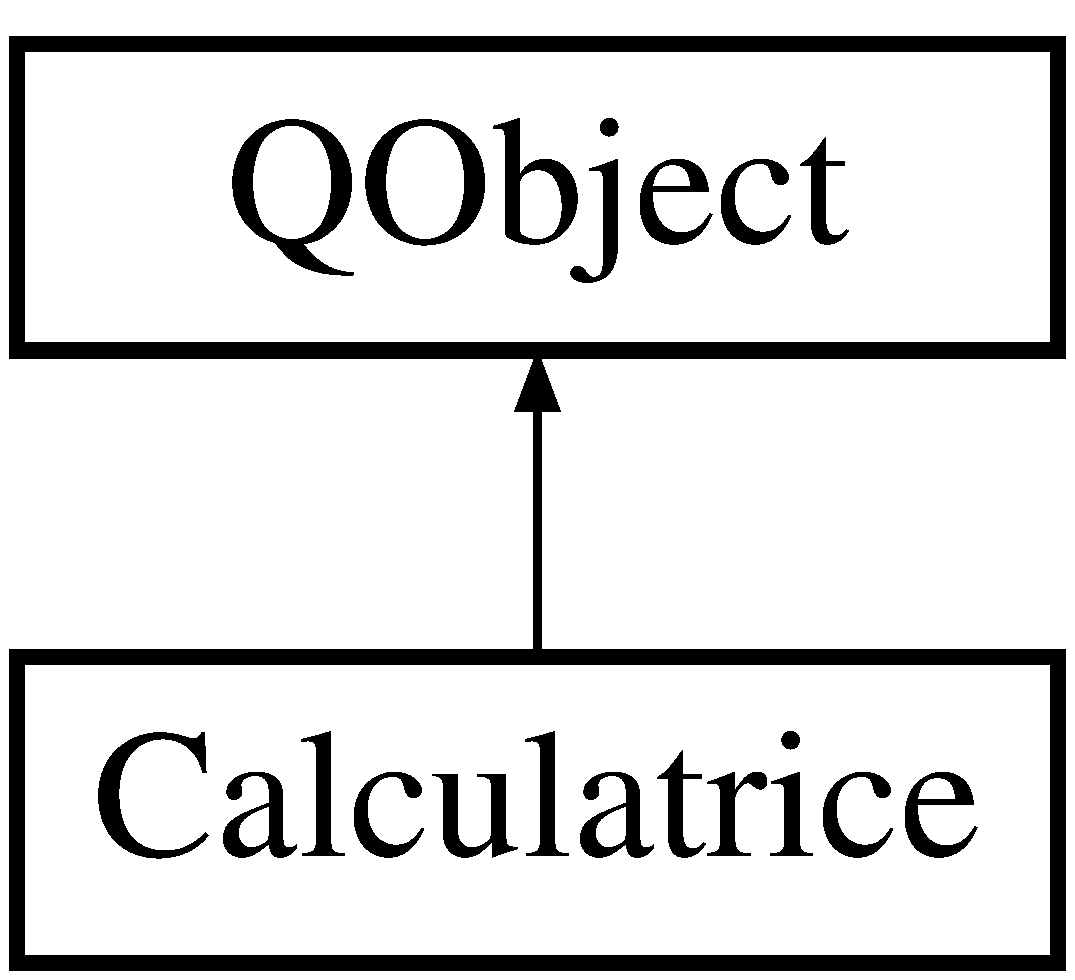
\includegraphics[height=2.000000cm]{class_calculatrice}
\end{center}
\end{figure}
\subsection*{Signals}
\begin{DoxyCompactItemize}
\item 
void \hyperlink{class_calculatrice_a5b379ff16856c59cd94d0f460b0d0d73}{new\+Atom} (const Q\+String \&, const Q\+String \&)
\begin{DoxyCompactList}\small\item\em \hyperlink{class_calculatrice_a5b379ff16856c59cd94d0f460b0d0d73}{new\+Atom()} Signal sent when a new Atome is created \end{DoxyCompactList}\item 
void \hyperlink{class_calculatrice_a5c1b210bef9aa7bd162478d35412b36b}{delete\+Atom} (const Q\+String \&, const Q\+String \&)
\begin{DoxyCompactList}\small\item\em \hyperlink{class_calculatrice_a5c1b210bef9aa7bd162478d35412b36b}{delete\+Atom()} Signal sent when a new Atome is created \end{DoxyCompactList}\end{DoxyCompactItemize}
\subsection*{Public Member Functions}
\begin{DoxyCompactItemize}
\item 
map$<$ Q\+String, \hyperlink{class_litterale}{Litterale} $\ast$ $>$ {\bfseries get\+Map\+Atome} () const \hypertarget{class_calculatrice_a7052dd37aa1976d3deef76e4a0ba8d79}{}\label{class_calculatrice_a7052dd37aa1976d3deef76e4a0ba8d79}

\item 
unsigned int {\bfseries get\+Nb\+Atoms} () const \hypertarget{class_calculatrice_a3a4fad24caff85518b77c61adc5e730e}{}\label{class_calculatrice_a3a4fad24caff85518b77c61adc5e730e}

\item 
\hyperlink{class_calculatrice_a2350ed13f91c824c7cd6c4a65ab42dde}{Calculatrice} (\hyperlink{class_pile}{Pile} $\ast$p)
\begin{DoxyCompactList}\small\item\em Constructor. \end{DoxyCompactList}\item 
\hyperlink{class_calculatrice_acb4b6278eb955ce932e16df29276be52}{$\sim$\+Calculatrice} ()
\begin{DoxyCompactList}\small\item\em Destructor. \end{DoxyCompactList}\item 
Q\+String \hyperlink{class_calculatrice_a05f1ea7ed7113ee8d4f92fd13d6e9591}{get\+Last\+Op} () const 
\begin{DoxyCompactList}\small\item\em \hyperlink{class_calculatrice_a05f1ea7ed7113ee8d4f92fd13d6e9591}{get\+Last\+Op()} method \end{DoxyCompactList}\item 
\hyperlink{class_litterale}{Litterale} $\ast$ \hyperlink{class_calculatrice_adb12970d2534774f003cc790b2a87f43}{get\+Last\+Arg1} () const 
\begin{DoxyCompactList}\small\item\em \hyperlink{class_calculatrice_adb12970d2534774f003cc790b2a87f43}{get\+Last\+Arg1()} method \end{DoxyCompactList}\item 
\hyperlink{class_litterale}{Litterale} $\ast$ \hyperlink{class_calculatrice_aeb2562cb73e9140652f3de990999e795}{get\+Last\+Arg2} () const 
\begin{DoxyCompactList}\small\item\em \hyperlink{class_calculatrice_aeb2562cb73e9140652f3de990999e795}{get\+Last\+Arg2()} method \end{DoxyCompactList}\item 
\hyperlink{class_pile}{Pile} $\ast$ \hyperlink{class_calculatrice_ae2d0c9c7d1d378d65d1cab56124d29c8}{get\+Pile} () const 
\begin{DoxyCompactList}\small\item\em \hyperlink{class_calculatrice_ae2d0c9c7d1d378d65d1cab56124d29c8}{get\+Pile()} method \end{DoxyCompactList}\item 
void \hyperlink{class_calculatrice_a48c8aa03ff4562c5794a62e4e485fc39}{operateur2} (const Q\+String \&s)
\begin{DoxyCompactList}\small\item\em \hyperlink{class_calculatrice_a48c8aa03ff4562c5794a62e4e485fc39}{operateur2()} method \end{DoxyCompactList}\item 
void \hyperlink{class_calculatrice_ae82762b5bb2cadd28af3534353ce0431}{operateur1} (const Q\+String \&s)
\begin{DoxyCompactList}\small\item\em \hyperlink{class_calculatrice_ae82762b5bb2cadd28af3534353ce0431}{operateur1()} method \end{DoxyCompactList}\item 
void \hyperlink{class_calculatrice_a567873272e220894b3ddc5909c20b0a7}{operateurp} (const Q\+String \&s)
\begin{DoxyCompactList}\small\item\em \hyperlink{class_calculatrice_a567873272e220894b3ddc5909c20b0a7}{operateurp()} method \end{DoxyCompactList}\item 
void \hyperlink{class_calculatrice_aeda02ec9d861a66f67d75757db227504}{enregistrer\+Last} (const Q\+String \&s)
\begin{DoxyCompactList}\small\item\em \hyperlink{class_calculatrice_aeda02ec9d861a66f67d75757db227504}{enregistrer\+Last()} method \end{DoxyCompactList}\item 
void \hyperlink{class_calculatrice_ae96458c336f6b14ead0ae2086828d9bb}{commande} (const Q\+String \&s)
\begin{DoxyCompactList}\small\item\em \hyperlink{class_calculatrice_ae96458c336f6b14ead0ae2086828d9bb}{commande()} method \end{DoxyCompactList}\item 
void \hyperlink{class_calculatrice_a18952ea12781a4b3ca6147ff10298db7}{executer} ()
\begin{DoxyCompactList}\small\item\em \hyperlink{class_calculatrice_a18952ea12781a4b3ca6147ff10298db7}{executer()} method \end{DoxyCompactList}\item 
void \hyperlink{class_calculatrice_a579462aa5abe19ab51bd9b7e8fb9c5a1}{Eval} (const Q\+String \&exp1)
\begin{DoxyCompactList}\small\item\em \hyperlink{class_calculatrice_a579462aa5abe19ab51bd9b7e8fb9c5a1}{Eval()} method. \end{DoxyCompactList}\item 
Q\+String \hyperlink{class_calculatrice_a0fcf62f423e31fd182a74b76bb90e47d}{infixe\+Postfixe} (const Q\+String \&s)
\begin{DoxyCompactList}\small\item\em \hyperlink{class_calculatrice_a0fcf62f423e31fd182a74b76bb90e47d}{infixe\+Postfixe()} method \end{DoxyCompactList}\item 
void \hyperlink{class_calculatrice_ae6b03960bfed7c9d96893124acf2ae67}{add\+Atom} (const Q\+String \&s, \hyperlink{class_litterale}{Litterale} $\ast$li)
\begin{DoxyCompactList}\small\item\em add\+Atome() method \end{DoxyCompactList}\item 
void \hyperlink{class_calculatrice_a34ab6178729e5906fb38ccb09122f5b4}{remove\+Atom} (const Q\+String \&s)
\begin{DoxyCompactList}\small\item\em remove\+Atome() method \end{DoxyCompactList}\item 
bool \hyperlink{class_calculatrice_aeae79a2854c5341568391fe6399526c4}{already\+Exists} (const Q\+String \&s)
\begin{DoxyCompactList}\small\item\em \hyperlink{class_calculatrice_aeae79a2854c5341568391fe6399526c4}{already\+Exists()} method \end{DoxyCompactList}\item 
void \hyperlink{class_calculatrice_a8d75e506f620a940f66ab15583da6020}{afficher\+Tous\+Atomes} () const 
\begin{DoxyCompactList}\small\item\em \hyperlink{class_calculatrice_a8d75e506f620a940f66ab15583da6020}{afficher\+Tous\+Atomes()} method \end{DoxyCompactList}\end{DoxyCompactItemize}


\subsection{Constructor \& Destructor Documentation}
\index{Calculatrice@{Calculatrice}!Calculatrice@{Calculatrice}}
\index{Calculatrice@{Calculatrice}!Calculatrice@{Calculatrice}}
\subsubsection[{\texorpdfstring{Calculatrice(\+Pile $\ast$p)}{Calculatrice(Pile *p)}}]{\setlength{\rightskip}{0pt plus 5cm}Calculatrice\+::\+Calculatrice (
\begin{DoxyParamCaption}
\item[{{\bf Pile} $\ast$}]{p}
\end{DoxyParamCaption}
)\hspace{0.3cm}{\ttfamily [inline]}}\hypertarget{class_calculatrice_a2350ed13f91c824c7cd6c4a65ab42dde}{}\label{class_calculatrice_a2350ed13f91c824c7cd6c4a65ab42dde}


Constructor. 

Constructor of the \hyperlink{class_calculatrice}{Calculatrice} class the stack is initialize with the argument lastoperateur is initialize with an empty Q\+String lastarg1 and lastarg2 with nullptr Inline method


\begin{DoxyParams}{Parameters}
{\em 1} & parameter of type Pile$\ast$ \\
\hline
\end{DoxyParams}
\index{Calculatrice@{Calculatrice}!````~Calculatrice@{$\sim$\+Calculatrice}}
\index{````~Calculatrice@{$\sim$\+Calculatrice}!Calculatrice@{Calculatrice}}
\subsubsection[{\texorpdfstring{$\sim$\+Calculatrice()}{~Calculatrice()}}]{\setlength{\rightskip}{0pt plus 5cm}Calculatrice\+::$\sim$\+Calculatrice (
\begin{DoxyParamCaption}
{}
\end{DoxyParamCaption}
)\hspace{0.3cm}{\ttfamily [inline]}}\hypertarget{class_calculatrice_acb4b6278eb955ce932e16df29276be52}{}\label{class_calculatrice_acb4b6278eb955ce932e16df29276be52}


Destructor. 

Destructor of the \hyperlink{class_calculatrice}{Calculatrice} class (inline method) Needed because we have to delete the stack which was allocated dynamically


\begin{DoxyParams}{Parameters}
{\em no} & parameter \\
\hline
\end{DoxyParams}


\subsection{Member Function Documentation}
\index{Calculatrice@{Calculatrice}!add\+Atom@{add\+Atom}}
\index{add\+Atom@{add\+Atom}!Calculatrice@{Calculatrice}}
\subsubsection[{\texorpdfstring{add\+Atom(const Q\+String \&s, Litterale $\ast$li)}{addAtom(const QString &s, Litterale *li)}}]{\setlength{\rightskip}{0pt plus 5cm}void Calculatrice\+::add\+Atom (
\begin{DoxyParamCaption}
\item[{const Q\+String \&}]{s, }
\item[{{\bf Litterale} $\ast$}]{li}
\end{DoxyParamCaption}
)}\hypertarget{class_calculatrice_ae6b03960bfed7c9d96893124acf2ae67}{}\label{class_calculatrice_ae6b03960bfed7c9d96893124acf2ae67}


add\+Atome() method 


\begin{DoxyParams}{Parameters}
{\em 2} & parameters of type const Q\+String\& and Litteral$\ast$ \\
\hline
\end{DoxyParams}
\begin{DoxyReturn}{Returns}
void
\end{DoxyReturn}
Use to add a new Atome Very easy thanks to the map If it already exists it will change its value if not, it creates it


\begin{DoxyParams}{Parameters}
{\em 2} & parameters of type const Q\+String\& and Litteral$\ast$ \\
\hline
\end{DoxyParams}
\begin{DoxyReturn}{Returns}
void 
\end{DoxyReturn}
\index{Calculatrice@{Calculatrice}!afficher\+Tous\+Atomes@{afficher\+Tous\+Atomes}}
\index{afficher\+Tous\+Atomes@{afficher\+Tous\+Atomes}!Calculatrice@{Calculatrice}}
\subsubsection[{\texorpdfstring{afficher\+Tous\+Atomes() const }{afficherTousAtomes() const }}]{\setlength{\rightskip}{0pt plus 5cm}void Calculatrice\+::afficher\+Tous\+Atomes (
\begin{DoxyParamCaption}
{}
\end{DoxyParamCaption}
) const}\hypertarget{class_calculatrice_a8d75e506f620a940f66ab15583da6020}{}\label{class_calculatrice_a8d75e506f620a940f66ab15583da6020}


\hyperlink{class_calculatrice_a8d75e506f620a940f66ab15583da6020}{afficher\+Tous\+Atomes()} method 


\begin{DoxyParams}{Parameters}
{\em const} & Qstring\& \\
\hline
\end{DoxyParams}
\begin{DoxyReturn}{Returns}
void
\end{DoxyReturn}
Method to display all the atomes that the calculator contains


\begin{DoxyParams}{Parameters}
{\em const} & Qstring\& \\
\hline
\end{DoxyParams}
\begin{DoxyReturn}{Returns}
void 
\end{DoxyReturn}
\index{Calculatrice@{Calculatrice}!already\+Exists@{already\+Exists}}
\index{already\+Exists@{already\+Exists}!Calculatrice@{Calculatrice}}
\subsubsection[{\texorpdfstring{already\+Exists(const Q\+String \&s)}{alreadyExists(const QString &s)}}]{\setlength{\rightskip}{0pt plus 5cm}bool Calculatrice\+::already\+Exists (
\begin{DoxyParamCaption}
\item[{const Q\+String \&}]{s}
\end{DoxyParamCaption}
)}\hypertarget{class_calculatrice_aeae79a2854c5341568391fe6399526c4}{}\label{class_calculatrice_aeae79a2854c5341568391fe6399526c4}


\hyperlink{class_calculatrice_aeae79a2854c5341568391fe6399526c4}{already\+Exists()} method 


\begin{DoxyParams}{Parameters}
{\em const} & Qstring\& \\
\hline
\end{DoxyParams}
\begin{DoxyReturn}{Returns}
bool
\end{DoxyReturn}
Used to know if an atome already exists


\begin{DoxyParams}{Parameters}
{\em const} & Qstring\& \\
\hline
\end{DoxyParams}
\begin{DoxyReturn}{Returns}
bool (true if already exists, false otherwise) 
\end{DoxyReturn}
\index{Calculatrice@{Calculatrice}!commande@{commande}}
\index{commande@{commande}!Calculatrice@{Calculatrice}}
\subsubsection[{\texorpdfstring{commande(const Q\+String \&s)}{commande(const QString &s)}}]{\setlength{\rightskip}{0pt plus 5cm}void Calculatrice\+::commande (
\begin{DoxyParamCaption}
\item[{const Q\+String \&}]{c}
\end{DoxyParamCaption}
)}\hypertarget{class_calculatrice_ae96458c336f6b14ead0ae2086828d9bb}{}\label{class_calculatrice_ae96458c336f6b14ead0ae2086828d9bb}


\hyperlink{class_calculatrice_ae96458c336f6b14ead0ae2086828d9bb}{commande()} method 


\begin{DoxyParams}{Parameters}
{\em const} & Q\+String\& s \\
\hline
\end{DoxyParams}
\begin{DoxyReturn}{Returns}
void
\end{DoxyReturn}
Method whichwas declare in the \hyperlink{class_calculatrice}{Calculatrice} class Takes one argument of type const Q\+String\& representing what the user entered in the calculator if it is an integer, it pushes a new \hyperlink{class_li_entiere}{Li\+Entiere} if it is a double type number, it pushes a new \hyperlink{class_li_reelle}{Li\+Reelle} if it is an expression, it pushes a new \hyperlink{class_li_expression}{Li\+Expression} if it is an Atome \+: if it did not exist before, it creates an Expression, and if it already existed, it pushes the \hyperlink{class_litterale}{Litterale} corresponding to this atome if it is an operator, it calls the appropriate function (operator1, operator2, operatorp) try ... catch block to catch all the excpetions thrown by the different function called


\begin{DoxyParams}{Parameters}
{\em const} & Q\+String\& s \\
\hline
\end{DoxyParams}
\begin{DoxyReturn}{Returns}
void 
\end{DoxyReturn}
\index{Calculatrice@{Calculatrice}!delete\+Atom@{delete\+Atom}}
\index{delete\+Atom@{delete\+Atom}!Calculatrice@{Calculatrice}}
\subsubsection[{\texorpdfstring{delete\+Atom}{deleteAtom}}]{\setlength{\rightskip}{0pt plus 5cm}void Calculatrice\+::delete\+Atom (
\begin{DoxyParamCaption}
\item[{const Q\+String \&}]{, }
\item[{const Q\+String \&}]{}
\end{DoxyParamCaption}
)\hspace{0.3cm}{\ttfamily [signal]}}\hypertarget{class_calculatrice_a5c1b210bef9aa7bd162478d35412b36b}{}\label{class_calculatrice_a5c1b210bef9aa7bd162478d35412b36b}


\hyperlink{class_calculatrice_a5c1b210bef9aa7bd162478d35412b36b}{delete\+Atom()} Signal sent when a new Atome is created 


\begin{DoxyParams}{Parameters}
{\em const\+Q\+String\&} & \\
\hline
\end{DoxyParams}
\begin{DoxyReturn}{Returns}
void 
\end{DoxyReturn}
\index{Calculatrice@{Calculatrice}!enregistrer\+Last@{enregistrer\+Last}}
\index{enregistrer\+Last@{enregistrer\+Last}!Calculatrice@{Calculatrice}}
\subsubsection[{\texorpdfstring{enregistrer\+Last(const Q\+String \&s)}{enregistrerLast(const QString &s)}}]{\setlength{\rightskip}{0pt plus 5cm}void Calculatrice\+::enregistrer\+Last (
\begin{DoxyParamCaption}
\item[{const Q\+String \&}]{s}
\end{DoxyParamCaption}
)}\hypertarget{class_calculatrice_aeda02ec9d861a66f67d75757db227504}{}\label{class_calculatrice_aeda02ec9d861a66f67d75757db227504}


\hyperlink{class_calculatrice_aeda02ec9d861a66f67d75757db227504}{enregistrer\+Last()} method 


\begin{DoxyParams}{Parameters}
{\em const} & Q\+String\& s \\
\hline
\end{DoxyParams}
\begin{DoxyReturn}{Returns}
void
\end{DoxyReturn}
Method declared in the \hyperlink{class_calculatrice}{Calculatrice} class Used to save the last operator used after each operation Used to save the last arguments after each operation (makes a copy and delete the old ones if they have not been pushed again)


\begin{DoxyParams}{Parameters}
{\em const} & Q\+String\& s \\
\hline
\end{DoxyParams}
\begin{DoxyReturn}{Returns}
void 
\end{DoxyReturn}
\index{Calculatrice@{Calculatrice}!Eval@{Eval}}
\index{Eval@{Eval}!Calculatrice@{Calculatrice}}
\subsubsection[{\texorpdfstring{Eval(const Q\+String \&exp1)}{Eval(const QString &exp1)}}]{\setlength{\rightskip}{0pt plus 5cm}void Calculatrice\+::\+Eval (
\begin{DoxyParamCaption}
\item[{const Q\+String \&}]{exp1}
\end{DoxyParamCaption}
)}\hypertarget{class_calculatrice_a579462aa5abe19ab51bd9b7e8fb9c5a1}{}\label{class_calculatrice_a579462aa5abe19ab51bd9b7e8fb9c5a1}


\hyperlink{class_calculatrice_a579462aa5abe19ab51bd9b7e8fb9c5a1}{Eval()} method. 


\begin{DoxyParams}{Parameters}
{\em const} & Q\+String\& \\
\hline
\end{DoxyParams}
\begin{DoxyReturn}{Returns}
void 
\end{DoxyReturn}
\index{Calculatrice@{Calculatrice}!executer@{executer}}
\index{executer@{executer}!Calculatrice@{Calculatrice}}
\subsubsection[{\texorpdfstring{executer()}{executer()}}]{\setlength{\rightskip}{0pt plus 5cm}void Calculatrice\+::executer (
\begin{DoxyParamCaption}
{}
\end{DoxyParamCaption}
)}\hypertarget{class_calculatrice_a18952ea12781a4b3ca6147ff10298db7}{}\label{class_calculatrice_a18952ea12781a4b3ca6147ff10298db7}


\hyperlink{class_calculatrice_a18952ea12781a4b3ca6147ff10298db7}{executer()} method 


\begin{DoxyParams}{Parameters}
{\em no} & parameter \\
\hline
\end{DoxyParams}
\begin{DoxyReturn}{Returns}
void
\end{DoxyReturn}
Method declared in the \hyperlink{class_calculatrice}{Calculatrice} class takes what the user entered and sends it to the commande function


\begin{DoxyParams}{Parameters}
{\em no} & parameter \\
\hline
\end{DoxyParams}
\begin{DoxyReturn}{Returns}
void 
\end{DoxyReturn}
\index{Calculatrice@{Calculatrice}!get\+Last\+Arg1@{get\+Last\+Arg1}}
\index{get\+Last\+Arg1@{get\+Last\+Arg1}!Calculatrice@{Calculatrice}}
\subsubsection[{\texorpdfstring{get\+Last\+Arg1() const }{getLastArg1() const }}]{\setlength{\rightskip}{0pt plus 5cm}{\bf Litterale}$\ast$ Calculatrice\+::get\+Last\+Arg1 (
\begin{DoxyParamCaption}
{}
\end{DoxyParamCaption}
) const\hspace{0.3cm}{\ttfamily [inline]}}\hypertarget{class_calculatrice_adb12970d2534774f003cc790b2a87f43}{}\label{class_calculatrice_adb12970d2534774f003cc790b2a87f43}


\hyperlink{class_calculatrice_adb12970d2534774f003cc790b2a87f43}{get\+Last\+Arg1()} method 

Accessor to lastarg1 Const inline method (attribut should not be modified)


\begin{DoxyParams}{Parameters}
{\em no} & parameter \\
\hline
\end{DoxyParams}
\begin{DoxyReturn}{Returns}
Litterale$\ast$ 
\end{DoxyReturn}
\index{Calculatrice@{Calculatrice}!get\+Last\+Arg2@{get\+Last\+Arg2}}
\index{get\+Last\+Arg2@{get\+Last\+Arg2}!Calculatrice@{Calculatrice}}
\subsubsection[{\texorpdfstring{get\+Last\+Arg2() const }{getLastArg2() const }}]{\setlength{\rightskip}{0pt plus 5cm}{\bf Litterale}$\ast$ Calculatrice\+::get\+Last\+Arg2 (
\begin{DoxyParamCaption}
{}
\end{DoxyParamCaption}
) const\hspace{0.3cm}{\ttfamily [inline]}}\hypertarget{class_calculatrice_aeb2562cb73e9140652f3de990999e795}{}\label{class_calculatrice_aeb2562cb73e9140652f3de990999e795}


\hyperlink{class_calculatrice_aeb2562cb73e9140652f3de990999e795}{get\+Last\+Arg2()} method 

Accessor to lastarg2 Const inline method (attribut should not be modified)


\begin{DoxyParams}{Parameters}
{\em no} & parameter \\
\hline
\end{DoxyParams}
\begin{DoxyReturn}{Returns}
Litterale$\ast$ 
\end{DoxyReturn}
\index{Calculatrice@{Calculatrice}!get\+Last\+Op@{get\+Last\+Op}}
\index{get\+Last\+Op@{get\+Last\+Op}!Calculatrice@{Calculatrice}}
\subsubsection[{\texorpdfstring{get\+Last\+Op() const }{getLastOp() const }}]{\setlength{\rightskip}{0pt plus 5cm}Q\+String Calculatrice\+::get\+Last\+Op (
\begin{DoxyParamCaption}
{}
\end{DoxyParamCaption}
) const\hspace{0.3cm}{\ttfamily [inline]}}\hypertarget{class_calculatrice_a05f1ea7ed7113ee8d4f92fd13d6e9591}{}\label{class_calculatrice_a05f1ea7ed7113ee8d4f92fd13d6e9591}


\hyperlink{class_calculatrice_a05f1ea7ed7113ee8d4f92fd13d6e9591}{get\+Last\+Op()} method 

Accessor to lastoperator Const inline method (attribut should not be modified)


\begin{DoxyParams}{Parameters}
{\em no} & parameter \\
\hline
\end{DoxyParams}
\begin{DoxyReturn}{Returns}
Q\+String 
\end{DoxyReturn}
\index{Calculatrice@{Calculatrice}!get\+Pile@{get\+Pile}}
\index{get\+Pile@{get\+Pile}!Calculatrice@{Calculatrice}}
\subsubsection[{\texorpdfstring{get\+Pile() const }{getPile() const }}]{\setlength{\rightskip}{0pt plus 5cm}{\bf Pile}$\ast$ Calculatrice\+::get\+Pile (
\begin{DoxyParamCaption}
{}
\end{DoxyParamCaption}
) const\hspace{0.3cm}{\ttfamily [inline]}}\hypertarget{class_calculatrice_ae2d0c9c7d1d378d65d1cab56124d29c8}{}\label{class_calculatrice_ae2d0c9c7d1d378d65d1cab56124d29c8}


\hyperlink{class_calculatrice_ae2d0c9c7d1d378d65d1cab56124d29c8}{get\+Pile()} method 

Accessor to the stack Const inline method (attribut should not be modified)


\begin{DoxyParams}{Parameters}
{\em no} & parameter \\
\hline
\end{DoxyParams}
\begin{DoxyReturn}{Returns}
Pile$\ast$ 
\end{DoxyReturn}
\index{Calculatrice@{Calculatrice}!infixe\+Postfixe@{infixe\+Postfixe}}
\index{infixe\+Postfixe@{infixe\+Postfixe}!Calculatrice@{Calculatrice}}
\subsubsection[{\texorpdfstring{infixe\+Postfixe(const Q\+String \&s)}{infixePostfixe(const QString &s)}}]{\setlength{\rightskip}{0pt plus 5cm}Q\+String Calculatrice\+::infixe\+Postfixe (
\begin{DoxyParamCaption}
\item[{const Q\+String \&}]{s}
\end{DoxyParamCaption}
)}\hypertarget{class_calculatrice_a0fcf62f423e31fd182a74b76bb90e47d}{}\label{class_calculatrice_a0fcf62f423e31fd182a74b76bb90e47d}


\hyperlink{class_calculatrice_a0fcf62f423e31fd182a74b76bb90e47d}{infixe\+Postfixe()} method 


\begin{DoxyParams}{Parameters}
{\em const} & Q\+String\& \\
\hline
\end{DoxyParams}
\begin{DoxyReturn}{Returns}
Q\+String
\end{DoxyReturn}
Method declared in the \hyperlink{class_calculatrice}{Calculatrice} class Used to transform an expression (not wrote in R\+PN) in a new expression in R\+PN that can be interpreted by the commande function It is, in some cases, a recursive function If it finds in the expression a operator with parentheses like D\+I\+V(e1,e2), it calls the function again on e1 and e2 it has one Q\+Stack, an to manage the other operator found when the function finds an operator, it pushes it on the top of the stack only if its priority is higher than the priority of the operator already on the top of the stack if its priority is lower, it adds it to \char`\"{}post\char`\"{} which is the Q\+String that the function will return if the function finds a number, it also adds it to post


\begin{DoxyParams}{Parameters}
{\em const} & Q\+String\& \\
\hline
\end{DoxyParams}
\begin{DoxyReturn}{Returns}
Q\+String 
\end{DoxyReturn}
\index{Calculatrice@{Calculatrice}!new\+Atom@{new\+Atom}}
\index{new\+Atom@{new\+Atom}!Calculatrice@{Calculatrice}}
\subsubsection[{\texorpdfstring{new\+Atom}{newAtom}}]{\setlength{\rightskip}{0pt plus 5cm}void Calculatrice\+::new\+Atom (
\begin{DoxyParamCaption}
\item[{const Q\+String \&}]{, }
\item[{const Q\+String \&}]{}
\end{DoxyParamCaption}
)\hspace{0.3cm}{\ttfamily [signal]}}\hypertarget{class_calculatrice_a5b379ff16856c59cd94d0f460b0d0d73}{}\label{class_calculatrice_a5b379ff16856c59cd94d0f460b0d0d73}


\hyperlink{class_calculatrice_a5b379ff16856c59cd94d0f460b0d0d73}{new\+Atom()} Signal sent when a new Atome is created 


\begin{DoxyParams}{Parameters}
{\em const\+Q\+String\&} & \\
\hline
\end{DoxyParams}
\begin{DoxyReturn}{Returns}
void 
\end{DoxyReturn}
\index{Calculatrice@{Calculatrice}!operateur1@{operateur1}}
\index{operateur1@{operateur1}!Calculatrice@{Calculatrice}}
\subsubsection[{\texorpdfstring{operateur1(const Q\+String \&s)}{operateur1(const QString &s)}}]{\setlength{\rightskip}{0pt plus 5cm}void Calculatrice\+::operateur1 (
\begin{DoxyParamCaption}
\item[{const Q\+String \&}]{s}
\end{DoxyParamCaption}
)}\hypertarget{class_calculatrice_ae82762b5bb2cadd28af3534353ce0431}{}\label{class_calculatrice_ae82762b5bb2cadd28af3534353ce0431}


\hyperlink{class_calculatrice_ae82762b5bb2cadd28af3534353ce0431}{operateur1()} method 


\begin{DoxyParams}{Parameters}
{\em const} & Q\+String\& s \\
\hline
\end{DoxyParams}
\begin{DoxyReturn}{Returns}
void
\end{DoxyReturn}
Method declared in the \hyperlink{class_calculatrice}{Calculatrice} class Used to manage all the operation with a unaire operator the binary operator are \+: N\+EG, N\+UM, D\+EN, RE, IM, N\+OT, F\+O\+R\+G\+ET It takes one \hyperlink{class_litterale}{Litterale} from the stack (pop and drop) Then the calls the appropriate operator which was overloaded in the other classes Throws an error when called on a wrong operator


\begin{DoxyParams}{Parameters}
{\em const} & Q\+String\& s \\
\hline
\end{DoxyParams}
\begin{DoxyReturn}{Returns}
void 
\end{DoxyReturn}
\index{Calculatrice@{Calculatrice}!operateur2@{operateur2}}
\index{operateur2@{operateur2}!Calculatrice@{Calculatrice}}
\subsubsection[{\texorpdfstring{operateur2(const Q\+String \&s)}{operateur2(const QString &s)}}]{\setlength{\rightskip}{0pt plus 5cm}void Calculatrice\+::operateur2 (
\begin{DoxyParamCaption}
\item[{const Q\+String \&}]{s}
\end{DoxyParamCaption}
)}\hypertarget{class_calculatrice_a48c8aa03ff4562c5794a62e4e485fc39}{}\label{class_calculatrice_a48c8aa03ff4562c5794a62e4e485fc39}


\hyperlink{class_calculatrice_a48c8aa03ff4562c5794a62e4e485fc39}{operateur2()} method 


\begin{DoxyParams}{Parameters}
{\em const} & Q\+String\& s \\
\hline
\end{DoxyParams}
\begin{DoxyReturn}{Returns}
void
\end{DoxyReturn}
Method declared in the \hyperlink{class_calculatrice}{Calculatrice} class Used to manage all the operation with a binary operator the binary operator are \+: +, -\/, $\ast$, /, D\+IV, M\+OD, \$, A\+ND, OR, , ==, !=, =$<$, $>$=, $<$, $>$ It takes two Litterales from the stack (pop and drop) Then the calls the appropriate operator which was overloaded in the other classes Throws an error when called on a wrong operator


\begin{DoxyParams}{Parameters}
{\em const} & Q\+String\& s \\
\hline
\end{DoxyParams}
\begin{DoxyReturn}{Returns}
void 
\end{DoxyReturn}
\index{Calculatrice@{Calculatrice}!operateurp@{operateurp}}
\index{operateurp@{operateurp}!Calculatrice@{Calculatrice}}
\subsubsection[{\texorpdfstring{operateurp(const Q\+String \&s)}{operateurp(const QString &s)}}]{\setlength{\rightskip}{0pt plus 5cm}void Calculatrice\+::operateurp (
\begin{DoxyParamCaption}
\item[{const Q\+String \&}]{s}
\end{DoxyParamCaption}
)}\hypertarget{class_calculatrice_a567873272e220894b3ddc5909c20b0a7}{}\label{class_calculatrice_a567873272e220894b3ddc5909c20b0a7}


\hyperlink{class_calculatrice_a567873272e220894b3ddc5909c20b0a7}{operateurp()} method 


\begin{DoxyParams}{Parameters}
{\em const} & Q\+String\& s \\
\hline
\end{DoxyParams}
\begin{DoxyReturn}{Returns}
void
\end{DoxyReturn}
Method declared in the \hyperlink{class_calculatrice}{Calculatrice} class Used to manage all the operation with a stack the binary operator are \+: N\+D\+UP, D\+R\+OP, S\+W\+AP, L\+A\+S\+T\+OP, L\+A\+S\+T\+A\+R\+GS, C\+L\+E\+AR For D\+UP, D\+R\+OP, S\+W\+AP, the function checks first if there is enough elements in the stack For L\+A\+S\+T\+OP it checks first if there is an operation to call (if yes, put it in the commande function) For L\+A\+S\+T\+A\+R\+GS, it push the last arguments only if they exist Throws an error when called on a wrong operator, or if there is any problem (not enough element in the stack, ...)


\begin{DoxyParams}{Parameters}
{\em const} & Q\+String\& s \\
\hline
\end{DoxyParams}
\begin{DoxyReturn}{Returns}
void 
\end{DoxyReturn}
\index{Calculatrice@{Calculatrice}!remove\+Atom@{remove\+Atom}}
\index{remove\+Atom@{remove\+Atom}!Calculatrice@{Calculatrice}}
\subsubsection[{\texorpdfstring{remove\+Atom(const Q\+String \&s)}{removeAtom(const QString &s)}}]{\setlength{\rightskip}{0pt plus 5cm}void Calculatrice\+::remove\+Atom (
\begin{DoxyParamCaption}
\item[{const Q\+String \&}]{s}
\end{DoxyParamCaption}
)}\hypertarget{class_calculatrice_a34ab6178729e5906fb38ccb09122f5b4}{}\label{class_calculatrice_a34ab6178729e5906fb38ccb09122f5b4}


remove\+Atome() method 


\begin{DoxyParams}{Parameters}
{\em const} & Q\+String\& \\
\hline
\end{DoxyParams}
\begin{DoxyReturn}{Returns}
void
\end{DoxyReturn}
Use to delete an atome use the erase method of map class


\begin{DoxyParams}{Parameters}
{\em 2} & parameters of type const Q\+String\& and Litteral$\ast$ \\
\hline
\end{DoxyParams}
\begin{DoxyReturn}{Returns}
void 
\end{DoxyReturn}


The documentation for this class was generated from the following files\+:\begin{DoxyCompactItemize}
\item 
\hyperlink{calculatrice_8h}{calculatrice.\+h}\item 
\hyperlink{calculatrice_8cpp}{calculatrice.\+cpp}\end{DoxyCompactItemize}

\hypertarget{class_pile_1_1iterator}{}\section{Pile\+:\+:iterator Class Reference}
\label{class_pile_1_1iterator}\index{Pile\+::iterator@{Pile\+::iterator}}


\hyperlink{class_the}{The} iterator class.  




{\ttfamily \#include $<$pile.\+h$>$}

\subsection*{Public Member Functions}
\begin{DoxyCompactItemize}
\item 
\hyperlink{class_pile_1_1iterator_a840f05175548dd9ac7bb595206f0044f}{iterator} ()\hypertarget{class_pile_1_1iterator_a840f05175548dd9ac7bb595206f0044f}{}\label{class_pile_1_1iterator_a840f05175548dd9ac7bb595206f0044f}

\begin{DoxyCompactList}\small\item\em iterator Public Constructor with no argument \end{DoxyCompactList}\item 
\hyperlink{class_litterale}{Litterale} \& \hyperlink{class_pile_1_1iterator_a5a84d0211e5cfb4ddb45661d7e940e87}{operator$\ast$} () const 
\begin{DoxyCompactList}\small\item\em overloaded operator $\ast$ \end{DoxyCompactList}\item 
bool \hyperlink{class_pile_1_1iterator_abfe0e25a2ebc5f3188c7a13f09d19129}{operator!=} (\hyperlink{class_pile_1_1iterator}{iterator} it) const 
\begin{DoxyCompactList}\small\item\em overloaded operator != \end{DoxyCompactList}\item 
\hyperlink{class_pile_1_1iterator}{iterator} \& \hyperlink{class_pile_1_1iterator_a05b171f7019504d6fb1b6a9a183bd75b}{operator++} ()
\begin{DoxyCompactList}\small\item\em overloaded operator ++ \end{DoxyCompactList}\item 
\hyperlink{class_pile_1_1iterator}{iterator} \& \hyperlink{class_pile_1_1iterator_a2885303b73c9f5aeaece13985d138773}{operator-\/-\/} ()
\begin{DoxyCompactList}\small\item\em overloaded operator -- \end{DoxyCompactList}\item 
bool \hyperlink{class_pile_1_1iterator_ae984b2c3b4144fbaad3f4e0540b3f9ab}{operator$>$=} (\hyperlink{class_pile_1_1iterator}{iterator} it)
\begin{DoxyCompactList}\small\item\em overloaded operator $>$= \end{DoxyCompactList}\end{DoxyCompactItemize}
\subsection*{Friends}
\begin{DoxyCompactItemize}
\item 
class {\bfseries Pile}\hypertarget{class_pile_1_1iterator_a77806361379cf369e95d2b4346c7e28a}{}\label{class_pile_1_1iterator_a77806361379cf369e95d2b4346c7e28a}

\end{DoxyCompactItemize}


\subsection{Detailed Description}
\hyperlink{class_the}{The} iterator class. 

Permits to go through the stack 

\subsection{Member Function Documentation}
\index{Pile\+::iterator@{Pile\+::iterator}!operator"!=@{operator"!=}}
\index{operator"!=@{operator"!=}!Pile\+::iterator@{Pile\+::iterator}}
\subsubsection[{\texorpdfstring{operator"!=(iterator it) const }{operator!=(iterator it) const }}]{\setlength{\rightskip}{0pt plus 5cm}bool Pile\+::iterator\+::operator!= (
\begin{DoxyParamCaption}
\item[{{\bf iterator}}]{it}
\end{DoxyParamCaption}
) const\hspace{0.3cm}{\ttfamily [inline]}}\hypertarget{class_pile_1_1iterator_abfe0e25a2ebc5f3188c7a13f09d19129}{}\label{class_pile_1_1iterator_abfe0e25a2ebc5f3188c7a13f09d19129}


overloaded operator != 

return true if the current \hyperlink{class_litterale}{Litterale} is different from the litteral from the iterator in parameter 
\begin{DoxyParams}{Parameters}
{\em an} & iterator \\
\hline
\end{DoxyParams}
\begin{DoxyReturn}{Returns}
a boolean 
\end{DoxyReturn}
\index{Pile\+::iterator@{Pile\+::iterator}!operator$\ast$@{operator$\ast$}}
\index{operator$\ast$@{operator$\ast$}!Pile\+::iterator@{Pile\+::iterator}}
\subsubsection[{\texorpdfstring{operator$\ast$() const }{operator*() const }}]{\setlength{\rightskip}{0pt plus 5cm}{\bf Litterale}\& Pile\+::iterator\+::operator$\ast$ (
\begin{DoxyParamCaption}
{}
\end{DoxyParamCaption}
) const\hspace{0.3cm}{\ttfamily [inline]}}\hypertarget{class_pile_1_1iterator_a5a84d0211e5cfb4ddb45661d7e940e87}{}\label{class_pile_1_1iterator_a5a84d0211e5cfb4ddb45661d7e940e87}


overloaded operator $\ast$ 

Get the current \hyperlink{class_litterale}{Litterale} while going threw the stack

\begin{DoxyReturn}{Returns}
a const reference to an object of class \hyperlink{class_litterale}{Litterale} 
\end{DoxyReturn}
\index{Pile\+::iterator@{Pile\+::iterator}!operator++@{operator++}}
\index{operator++@{operator++}!Pile\+::iterator@{Pile\+::iterator}}
\subsubsection[{\texorpdfstring{operator++()}{operator++()}}]{\setlength{\rightskip}{0pt plus 5cm}{\bf iterator}\& Pile\+::iterator\+::operator++ (
\begin{DoxyParamCaption}
{}
\end{DoxyParamCaption}
)\hspace{0.3cm}{\ttfamily [inline]}}\hypertarget{class_pile_1_1iterator_a05b171f7019504d6fb1b6a9a183bd75b}{}\label{class_pile_1_1iterator_a05b171f7019504d6fb1b6a9a183bd75b}


overloaded operator ++ 

return the next element in the stack

\begin{DoxyReturn}{Returns}
an iterator 
\end{DoxyReturn}
\index{Pile\+::iterator@{Pile\+::iterator}!operator-\/-\/@{operator-\/-\/}}
\index{operator-\/-\/@{operator-\/-\/}!Pile\+::iterator@{Pile\+::iterator}}
\subsubsection[{\texorpdfstring{operator-\/-\/()}{operator--()}}]{\setlength{\rightskip}{0pt plus 5cm}{\bf iterator}\& Pile\+::iterator\+::operator-\/-\/ (
\begin{DoxyParamCaption}
{}
\end{DoxyParamCaption}
)\hspace{0.3cm}{\ttfamily [inline]}}\hypertarget{class_pile_1_1iterator_a2885303b73c9f5aeaece13985d138773}{}\label{class_pile_1_1iterator_a2885303b73c9f5aeaece13985d138773}


overloaded operator -- 

return the past element in the stack

\begin{DoxyReturn}{Returns}
an iterator 
\end{DoxyReturn}
\index{Pile\+::iterator@{Pile\+::iterator}!operator$>$=@{operator$>$=}}
\index{operator$>$=@{operator$>$=}!Pile\+::iterator@{Pile\+::iterator}}
\subsubsection[{\texorpdfstring{operator$>$=(iterator it)}{operator>=(iterator it)}}]{\setlength{\rightskip}{0pt plus 5cm}bool Pile\+::iterator\+::operator$>$= (
\begin{DoxyParamCaption}
\item[{{\bf iterator}}]{it}
\end{DoxyParamCaption}
)\hspace{0.3cm}{\ttfamily [inline]}}\hypertarget{class_pile_1_1iterator_ae984b2c3b4144fbaad3f4e0540b3f9ab}{}\label{class_pile_1_1iterator_ae984b2c3b4144fbaad3f4e0540b3f9ab}


overloaded operator $>$= 

return true if current litteral $>$= litteral from the iterator in parameter 
\begin{DoxyParams}{Parameters}
{\em an} & iterator \\
\hline
\end{DoxyParams}
\begin{DoxyReturn}{Returns}
a boolean 
\end{DoxyReturn}


The documentation for this class was generated from the following file\+:\begin{DoxyCompactItemize}
\item 
\hyperlink{pile_8h}{pile.\+h}\end{DoxyCompactItemize}

\hypertarget{class_li_complexe}{}\section{Li\+Complexe Class Reference}
\label{class_li_complexe}\index{Li\+Complexe@{Li\+Complexe}}
Inheritance diagram for Li\+Complexe\+:\begin{figure}[H]
\begin{center}
\leavevmode
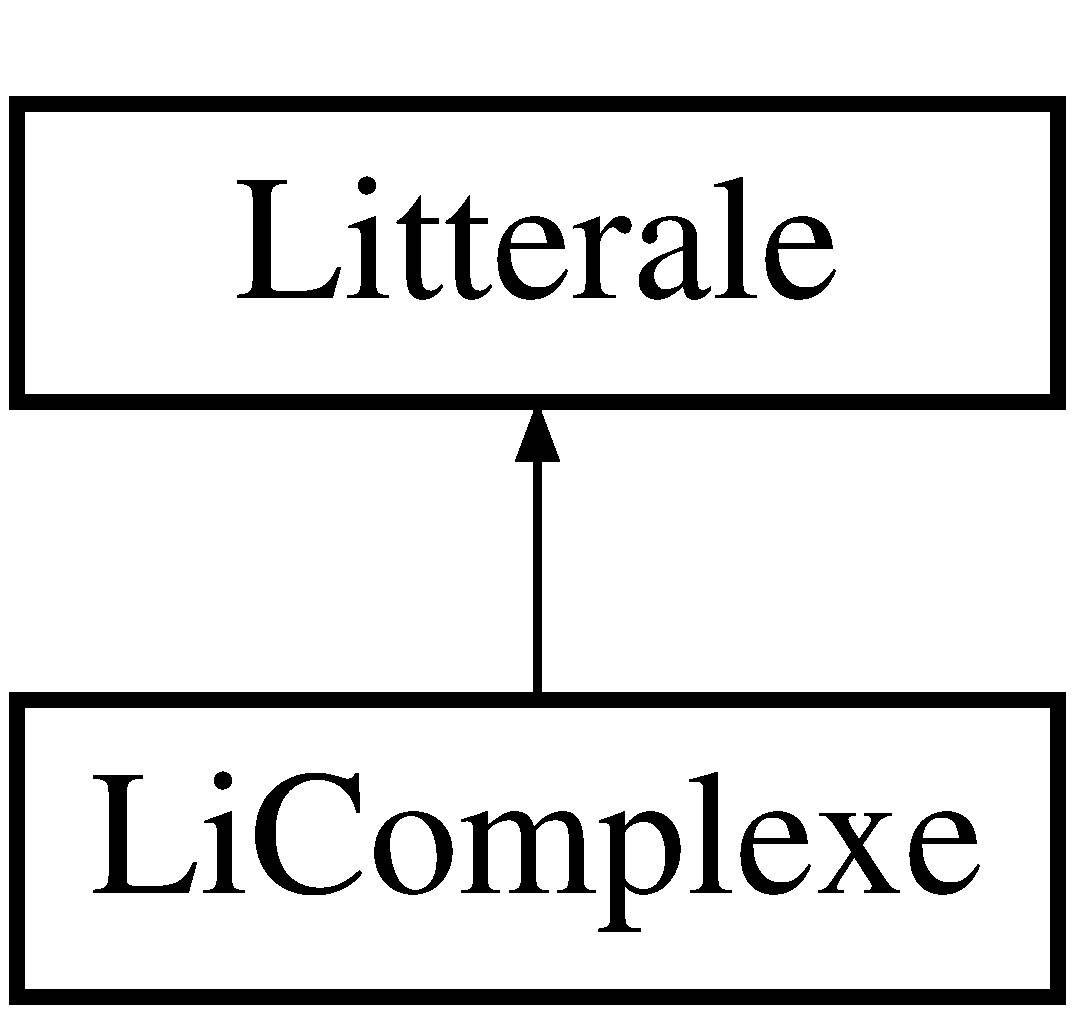
\includegraphics[height=2.000000cm]{class_li_complexe}
\end{center}
\end{figure}
\subsection*{Public Member Functions}
\begin{DoxyCompactItemize}
\item 
\hyperlink{class_li_complexe_a0681209fab64a65ed4da984218b3abfd}{Li\+Complexe} (\hyperlink{class_li_numerique}{Li\+Numerique} $\ast$r, \hyperlink{class_li_numerique}{Li\+Numerique} $\ast$i)
\begin{DoxyCompactList}\small\item\em Constructor. \end{DoxyCompactList}\item 
\hyperlink{class_li_complexe_a7acf3c859eca3cf2a8e6d81c05aa49d4}{Li\+Complexe} (const \hyperlink{class_li_complexe}{Li\+Complexe} \&lc)
\begin{DoxyCompactList}\small\item\em Copy Constructor. \end{DoxyCompactList}\item 
\hyperlink{class_li_complexe}{Li\+Complexe} \& \hyperlink{class_li_complexe_a5183c5901d1582f325b7f02f1b4f0198}{operator=} (const \hyperlink{class_li_complexe}{Li\+Complexe} \&lc)
\begin{DoxyCompactList}\small\item\em Assignment operator (operator=) \end{DoxyCompactList}\item 
\hyperlink{class_li_complexe_a56e0f48b9815525913fcf136e51ac39d}{$\sim$\+Li\+Complexe} ()
\begin{DoxyCompactList}\small\item\em Destructor. \end{DoxyCompactList}\item 
string \hyperlink{class_li_complexe_a5490d27f24fd273c8a3f5cc28e22d6d8}{to\+String} () const 
\begin{DoxyCompactList}\small\item\em \hyperlink{class_li_complexe_a5490d27f24fd273c8a3f5cc28e22d6d8}{to\+String()} method \end{DoxyCompactList}\item 
bool \hyperlink{class_li_complexe_a6bcabbf5bcf296fdb048c9be278f175a}{is\+Zero} () const 
\begin{DoxyCompactList}\small\item\em \hyperlink{class_li_complexe_a6bcabbf5bcf296fdb048c9be278f175a}{is\+Zero()} method \end{DoxyCompactList}\item 
\hyperlink{class_li_numerique}{Li\+Numerique} \& \hyperlink{class_li_complexe_abd5cae3001a94af1c18f7bb5092c9527}{get\+Reelle} () const 
\begin{DoxyCompactList}\small\item\em \hyperlink{class_li_complexe_abd5cae3001a94af1c18f7bb5092c9527}{get\+Reelle()} method \end{DoxyCompactList}\item 
\hyperlink{class_li_numerique}{Li\+Numerique} \& \hyperlink{class_li_complexe_ab0984cadf03a19e440dce8cea70b86e0}{get\+Image} () const 
\begin{DoxyCompactList}\small\item\em \hyperlink{class_li_complexe_abd5cae3001a94af1c18f7bb5092c9527}{get\+Reelle()} method \end{DoxyCompactList}\item 
\hyperlink{class_litterale}{Litterale} $\ast$ \hyperlink{class_li_complexe_a10fc45528f4f674e5afdddcd49cfefe8}{operator+} (const \hyperlink{class_litterale}{Litterale} \&li) const 
\begin{DoxyCompactList}\small\item\em overloaded operator+ \end{DoxyCompactList}\item 
\hyperlink{class_litterale}{Litterale} $\ast$ \hyperlink{class_li_complexe_aafe560e78d42938bce8e42672850f187}{operator-\/} (const \hyperlink{class_litterale}{Litterale} \&li) const 
\begin{DoxyCompactList}\small\item\em overloaded operator-\/ \end{DoxyCompactList}\item 
\hyperlink{class_litterale}{Litterale} $\ast$ \hyperlink{class_li_complexe_ab9dbace3f0fbd634a6258c4bcb5dc659}{operator/} (const \hyperlink{class_litterale}{Litterale} \&li) const 
\begin{DoxyCompactList}\small\item\em overloaded operator/ \end{DoxyCompactList}\item 
\hyperlink{class_litterale}{Litterale} $\ast$ \hyperlink{class_li_complexe_a88ad289cf55d8e6d89f0d77cf09d2ccf}{operator$\ast$} (const \hyperlink{class_litterale}{Litterale} \&li) const 
\begin{DoxyCompactList}\small\item\em overloaded operator$\ast$ \end{DoxyCompactList}\item 
\hyperlink{class_litterale}{Litterale} $\ast$ \hyperlink{class_li_complexe_a80fb4bf75402d5d1b8f1a3b9622b9047}{operator==} (const \hyperlink{class_litterale}{Litterale} \&li) const 
\begin{DoxyCompactList}\small\item\em overloaded operator== \end{DoxyCompactList}\item 
\hyperlink{class_litterale}{Litterale} $\ast$ \hyperlink{class_li_complexe_a85020ff32c533327425c70ebbf804abf}{operator!=} (const \hyperlink{class_litterale}{Litterale} \&li) const 
\begin{DoxyCompactList}\small\item\em overloaded operator!= \end{DoxyCompactList}\item 
\hyperlink{class_litterale}{Litterale} $\ast$ \hyperlink{class_li_complexe_ae749d5d340b4bf8e878442a38caa78c1}{operator$<$=} (const \hyperlink{class_litterale}{Litterale} \&li) const 
\begin{DoxyCompactList}\small\item\em overloaded operator$<$= \end{DoxyCompactList}\item 
\hyperlink{class_litterale}{Litterale} $\ast$ \hyperlink{class_li_complexe_a5c67194eb76e8760ce6dfec0e89f477a}{operator$>$=} (const \hyperlink{class_litterale}{Litterale} \&li) const 
\begin{DoxyCompactList}\small\item\em overloaded operator$>$= \end{DoxyCompactList}\item 
\hyperlink{class_litterale}{Litterale} $\ast$ \hyperlink{class_li_complexe_acb3d4e0f6636270f861490c465d07711}{operator$<$} (const \hyperlink{class_litterale}{Litterale} \&li) const 
\begin{DoxyCompactList}\small\item\em overloaded operator$<$ \end{DoxyCompactList}\item 
\hyperlink{class_litterale}{Litterale} $\ast$ \hyperlink{class_li_complexe_a8b7b532a469c8e2abe976070d7433666}{operator$>$} (const \hyperlink{class_litterale}{Litterale} \&li) const 
\begin{DoxyCompactList}\small\item\em overloaded operator$>$ \end{DoxyCompactList}\item 
\hyperlink{class_li_complexe}{Li\+Complexe} $\ast$ \hyperlink{class_li_complexe_a71954f11bfc89933860279cb932f68a9}{Neg} ()
\begin{DoxyCompactList}\small\item\em N\+E\+G() method. \end{DoxyCompactList}\item 
\hyperlink{class_litterale}{Litterale} $\ast$ \hyperlink{class_li_complexe_a7068b0171c0e0efb6ba803247f1aceca}{Num} ()
\begin{DoxyCompactList}\small\item\em N\+U\+M() method. \end{DoxyCompactList}\item 
\hyperlink{class_litterale}{Litterale} $\ast$ \hyperlink{class_li_complexe_aa4f828dac7bc5fbea088a289719943b6}{Den} ()
\begin{DoxyCompactList}\small\item\em D\+E\+N() method. \end{DoxyCompactList}\item 
\hyperlink{class_litterale}{Litterale} $\ast$ \hyperlink{class_li_complexe_ad93d70af2512c0e835c29677c12c419a}{Re} ()
\begin{DoxyCompactList}\small\item\em R\+E() method. \end{DoxyCompactList}\item 
\hyperlink{class_litterale}{Litterale} $\ast$ \hyperlink{class_li_complexe_a57082c43306e5d43c69d037723d646e7}{Im} ()
\begin{DoxyCompactList}\small\item\em I\+M() method. \end{DoxyCompactList}\item 
\hyperlink{class_litterale}{Litterale} $\ast$ \hyperlink{class_li_complexe_acf2840a901081b436f43045660d14362}{And} (const \hyperlink{class_litterale}{Litterale} $\ast$li)
\begin{DoxyCompactList}\small\item\em A\+N\+D() method. \end{DoxyCompactList}\item 
\hyperlink{class_litterale}{Litterale} $\ast$ \hyperlink{class_li_complexe_a4e05098ec1cdc4b6fd8bba10875181dd}{Or} (const \hyperlink{class_litterale}{Litterale} $\ast$li)
\begin{DoxyCompactList}\small\item\em O\+R() method. \end{DoxyCompactList}\item 
\hyperlink{class_litterale}{Litterale} $\ast$ \hyperlink{class_li_complexe_a37011cb1b7e5d4e9a2e22f217eb463f2}{Not} ()
\begin{DoxyCompactList}\small\item\em N\+O\+T() method. \end{DoxyCompactList}\item 
\hyperlink{class_litterale}{Litterale} $\ast$ {\bfseries Clone} () const \hypertarget{class_li_complexe_a0a55a686e7db1523bdbf95e5b146646f}{}\label{class_li_complexe_a0a55a686e7db1523bdbf95e5b146646f}

\end{DoxyCompactItemize}


\subsection{Constructor \& Destructor Documentation}
\index{Li\+Complexe@{Li\+Complexe}!Li\+Complexe@{Li\+Complexe}}
\index{Li\+Complexe@{Li\+Complexe}!Li\+Complexe@{Li\+Complexe}}
\subsubsection[{\texorpdfstring{Li\+Complexe(\+Li\+Numerique $\ast$r, Li\+Numerique $\ast$i)}{LiComplexe(LiNumerique *r, LiNumerique *i)}}]{\setlength{\rightskip}{0pt plus 5cm}Li\+Complexe\+::\+Li\+Complexe (
\begin{DoxyParamCaption}
\item[{{\bf Li\+Numerique} $\ast$}]{r, }
\item[{{\bf Li\+Numerique} $\ast$}]{i}
\end{DoxyParamCaption}
)}\hypertarget{class_li_complexe_a0681209fab64a65ed4da984218b3abfd}{}\label{class_li_complexe_a0681209fab64a65ed4da984218b3abfd}


Constructor. 


\begin{DoxyParams}{Parameters}
{\em 2} & parameters of type Li\+Numerique$\ast$, to initialize the real and the imaginary part\\
\hline
\end{DoxyParams}
Constructor of the \hyperlink{class_li_complexe}{Li\+Complexe} class Needed because the attributes are pointers, so we have to make a copy


\begin{DoxyParams}{Parameters}
{\em 2} & parameters of type Li\+Numerique$\ast$, to initialize the real and the imaginary part \\
\hline
\end{DoxyParams}
\index{Li\+Complexe@{Li\+Complexe}!Li\+Complexe@{Li\+Complexe}}
\index{Li\+Complexe@{Li\+Complexe}!Li\+Complexe@{Li\+Complexe}}
\subsubsection[{\texorpdfstring{Li\+Complexe(const Li\+Complexe \&lc)}{LiComplexe(const LiComplexe &lc)}}]{\setlength{\rightskip}{0pt plus 5cm}Li\+Complexe\+::\+Li\+Complexe (
\begin{DoxyParamCaption}
\item[{const {\bf Li\+Complexe} \&}]{lc}
\end{DoxyParamCaption}
)}\hypertarget{class_li_complexe_a7acf3c859eca3cf2a8e6d81c05aa49d4}{}\label{class_li_complexe_a7acf3c859eca3cf2a8e6d81c05aa49d4}


Copy Constructor. 


\begin{DoxyParams}{Parameters}
{\em 1} & parameter of type const \hyperlink{class_li_complexe}{Li\+Complexe}\& (needed because the attributs are pointers to Li\+Numerique$\ast$\\
\hline
\end{DoxyParams}
Copy Constructor of the \hyperlink{class_li_complexe}{Li\+Complexe} class Needed ecause the attributes are pointers, so we have to make a copy


\begin{DoxyParams}{Parameters}
{\em 1} & parameter of type const \hyperlink{class_li_complexe}{Li\+Complexe}\& \\
\hline
\end{DoxyParams}
\index{Li\+Complexe@{Li\+Complexe}!````~Li\+Complexe@{$\sim$\+Li\+Complexe}}
\index{````~Li\+Complexe@{$\sim$\+Li\+Complexe}!Li\+Complexe@{Li\+Complexe}}
\subsubsection[{\texorpdfstring{$\sim$\+Li\+Complexe()}{~LiComplexe()}}]{\setlength{\rightskip}{0pt plus 5cm}Li\+Complexe\+::$\sim$\+Li\+Complexe (
\begin{DoxyParamCaption}
{}
\end{DoxyParamCaption}
)\hspace{0.3cm}{\ttfamily [inline]}}\hypertarget{class_li_complexe_a56e0f48b9815525913fcf136e51ac39d}{}\label{class_li_complexe_a56e0f48b9815525913fcf136e51ac39d}


Destructor. 

Destructor of the \hyperlink{class_li_complexe}{Li\+Complexe} class Inline Method


\begin{DoxyParams}{Parameters}
{\em 1} & no parameters Delete the attributes that are allocated dynamically \\
\hline
\end{DoxyParams}


\subsection{Member Function Documentation}
\index{Li\+Complexe@{Li\+Complexe}!And@{And}}
\index{And@{And}!Li\+Complexe@{Li\+Complexe}}
\subsubsection[{\texorpdfstring{And(const Litterale $\ast$li)}{And(const Litterale *li)}}]{\setlength{\rightskip}{0pt plus 5cm}{\bf Litterale} $\ast$ Li\+Complexe\+::\+And (
\begin{DoxyParamCaption}
\item[{const {\bf Litterale} $\ast$}]{li}
\end{DoxyParamCaption}
)\hspace{0.3cm}{\ttfamily [virtual]}}\hypertarget{class_li_complexe_acf2840a901081b436f43045660d14362}{}\label{class_li_complexe_acf2840a901081b436f43045660d14362}


A\+N\+D() method. 


\begin{DoxyParams}{Parameters}
{\em const} & reference to \hyperlink{class_litterale}{Litterale} \\
\hline
\end{DoxyParams}
\begin{DoxyReturn}{Returns}
pointer to \hyperlink{class_litterale}{Litterale} \+: \hyperlink{class_li_entiere}{Li\+Entiere(1)} if true, \hyperlink{class_li_entiere}{Li\+Entiere(0)} if false
\end{DoxyReturn}
Method which was defined in \hyperlink{class_litterale}{Litterale} (pure virtual) Logic operator and


\begin{DoxyParams}{Parameters}
{\em const} & reference to \hyperlink{class_litterale}{Litterale} \\
\hline
\end{DoxyParams}
\begin{DoxyReturn}{Returns}
pointer to \hyperlink{class_litterale}{Litterale} \+: \hyperlink{class_li_entiere}{Li\+Entiere(1)} if true, \hyperlink{class_li_entiere}{Li\+Entiere(0)} if false 
\end{DoxyReturn}


Implements \hyperlink{class_litterale_a2331619771c5cb74bee253e2c2cf62f5}{Litterale}.

\index{Li\+Complexe@{Li\+Complexe}!Den@{Den}}
\index{Den@{Den}!Li\+Complexe@{Li\+Complexe}}
\subsubsection[{\texorpdfstring{Den()}{Den()}}]{\setlength{\rightskip}{0pt plus 5cm}{\bf Litterale}$\ast$ Li\+Complexe\+::\+Den (
\begin{DoxyParamCaption}
{}
\end{DoxyParamCaption}
)\hspace{0.3cm}{\ttfamily [inline]}, {\ttfamily [virtual]}}\hypertarget{class_li_complexe_aa4f828dac7bc5fbea088a289719943b6}{}\label{class_li_complexe_aa4f828dac7bc5fbea088a289719943b6}


D\+E\+N() method. 

Method which was defined in \hyperlink{class_litterale}{Litterale} (pure virtual) Throws an error used on a Lireelle (can only be used on \hyperlink{class_li_rationnelle}{Li\+Rationnelle} to return the denominator) Inline Method


\begin{DoxyParams}{Parameters}
{\em no} & parameter \\
\hline
\end{DoxyParams}
\begin{DoxyReturn}{Returns}
pointer to \hyperlink{class_litterale}{Litterale} 
\end{DoxyReturn}


Implements \hyperlink{class_litterale_aedcaa806cc6b037371b25d12086503b8}{Litterale}.

\index{Li\+Complexe@{Li\+Complexe}!get\+Image@{get\+Image}}
\index{get\+Image@{get\+Image}!Li\+Complexe@{Li\+Complexe}}
\subsubsection[{\texorpdfstring{get\+Image() const }{getImage() const }}]{\setlength{\rightskip}{0pt plus 5cm}{\bf Li\+Numerique}\& Li\+Complexe\+::get\+Image (
\begin{DoxyParamCaption}
{}
\end{DoxyParamCaption}
) const\hspace{0.3cm}{\ttfamily [inline]}}\hypertarget{class_li_complexe_ab0984cadf03a19e440dce8cea70b86e0}{}\label{class_li_complexe_ab0984cadf03a19e440dce8cea70b86e0}


\hyperlink{class_li_complexe_abd5cae3001a94af1c18f7bb5092c9527}{get\+Reelle()} method 

Accessor to the imaginary part of a \hyperlink{class_li_complexe}{Li\+Complexe} Inline Method


\begin{DoxyParams}{Parameters}
{\em no} & parameter \\
\hline
\end{DoxyParams}
\begin{DoxyReturn}{Returns}
reference to \hyperlink{class_li_numerique}{Li\+Numerique} 
\end{DoxyReturn}
\index{Li\+Complexe@{Li\+Complexe}!get\+Reelle@{get\+Reelle}}
\index{get\+Reelle@{get\+Reelle}!Li\+Complexe@{Li\+Complexe}}
\subsubsection[{\texorpdfstring{get\+Reelle() const }{getReelle() const }}]{\setlength{\rightskip}{0pt plus 5cm}{\bf Li\+Numerique}\& Li\+Complexe\+::get\+Reelle (
\begin{DoxyParamCaption}
{}
\end{DoxyParamCaption}
) const\hspace{0.3cm}{\ttfamily [inline]}}\hypertarget{class_li_complexe_abd5cae3001a94af1c18f7bb5092c9527}{}\label{class_li_complexe_abd5cae3001a94af1c18f7bb5092c9527}


\hyperlink{class_li_complexe_abd5cae3001a94af1c18f7bb5092c9527}{get\+Reelle()} method 

Accessor to the real part of a \hyperlink{class_li_complexe}{Li\+Complexe} Inline Method


\begin{DoxyParams}{Parameters}
{\em no} & parameter \\
\hline
\end{DoxyParams}
\begin{DoxyReturn}{Returns}
reference to \hyperlink{class_li_numerique}{Li\+Numerique} 
\end{DoxyReturn}
\index{Li\+Complexe@{Li\+Complexe}!Im@{Im}}
\index{Im@{Im}!Li\+Complexe@{Li\+Complexe}}
\subsubsection[{\texorpdfstring{Im()}{Im()}}]{\setlength{\rightskip}{0pt plus 5cm}{\bf Litterale}$\ast$ Li\+Complexe\+::\+Im (
\begin{DoxyParamCaption}
{}
\end{DoxyParamCaption}
)\hspace{0.3cm}{\ttfamily [inline]}, {\ttfamily [virtual]}}\hypertarget{class_li_complexe_a57082c43306e5d43c69d037723d646e7}{}\label{class_li_complexe_a57082c43306e5d43c69d037723d646e7}


I\+M() method. 

Method which was defined in \hyperlink{class_litterale}{Litterale} (pure virtual) Accessor to the imaginary part of a \hyperlink{class_li_complexe}{Li\+Complexe} Inline Method


\begin{DoxyParams}{Parameters}
{\em no} & parameter \\
\hline
\end{DoxyParams}
\begin{DoxyReturn}{Returns}
pointer to \hyperlink{class_litterale}{Litterale} 
\end{DoxyReturn}


Implements \hyperlink{class_litterale_a8f0c2d98186c545f4f34ae07b9751f97}{Litterale}.

\index{Li\+Complexe@{Li\+Complexe}!is\+Zero@{is\+Zero}}
\index{is\+Zero@{is\+Zero}!Li\+Complexe@{Li\+Complexe}}
\subsubsection[{\texorpdfstring{is\+Zero() const }{isZero() const }}]{\setlength{\rightskip}{0pt plus 5cm}bool Li\+Complexe\+::is\+Zero (
\begin{DoxyParamCaption}
{}
\end{DoxyParamCaption}
) const\hspace{0.3cm}{\ttfamily [inline]}, {\ttfamily [virtual]}}\hypertarget{class_li_complexe_a6bcabbf5bcf296fdb048c9be278f175a}{}\label{class_li_complexe_a6bcabbf5bcf296fdb048c9be278f175a}


\hyperlink{class_li_complexe_a6bcabbf5bcf296fdb048c9be278f175a}{is\+Zero()} method 

Pure virtual method in \hyperlink{class_litterale}{Litterale}, used to test if re and im are equal to 0 Use the is\+Zero mehtods defined in the other classes Inline Method


\begin{DoxyParams}{Parameters}
{\em no} & parameter \\
\hline
\end{DoxyParams}
\begin{DoxyReturn}{Returns}
bool 
\end{DoxyReturn}


Implements \hyperlink{class_litterale_a535fc431d96954754b7a729404df4a79}{Litterale}.

\index{Li\+Complexe@{Li\+Complexe}!Neg@{Neg}}
\index{Neg@{Neg}!Li\+Complexe@{Li\+Complexe}}
\subsubsection[{\texorpdfstring{Neg()}{Neg()}}]{\setlength{\rightskip}{0pt plus 5cm}{\bf Li\+Complexe}$\ast$ Li\+Complexe\+::\+Neg (
\begin{DoxyParamCaption}
{}
\end{DoxyParamCaption}
)\hspace{0.3cm}{\ttfamily [inline]}, {\ttfamily [virtual]}}\hypertarget{class_li_complexe_a71954f11bfc89933860279cb932f68a9}{}\label{class_li_complexe_a71954f11bfc89933860279cb932f68a9}


N\+E\+G() method. 

Method which was defined in \hyperlink{class_litterale}{Litterale} (pure virtual) Used to change the sign of value Inline Method


\begin{DoxyParams}{Parameters}
{\em no} & parameter \\
\hline
\end{DoxyParams}
\begin{DoxyReturn}{Returns}
pointer to \hyperlink{class_li_reelle}{Li\+Reelle} 
\end{DoxyReturn}


Implements \hyperlink{class_litterale_ac9261e971a9d7d84137557d1cad94336}{Litterale}.

\index{Li\+Complexe@{Li\+Complexe}!Not@{Not}}
\index{Not@{Not}!Li\+Complexe@{Li\+Complexe}}
\subsubsection[{\texorpdfstring{Not()}{Not()}}]{\setlength{\rightskip}{0pt plus 5cm}{\bf Litterale} $\ast$ Li\+Complexe\+::\+Not (
\begin{DoxyParamCaption}
{}
\end{DoxyParamCaption}
)\hspace{0.3cm}{\ttfamily [virtual]}}\hypertarget{class_li_complexe_a37011cb1b7e5d4e9a2e22f217eb463f2}{}\label{class_li_complexe_a37011cb1b7e5d4e9a2e22f217eb463f2}


N\+O\+T() method. 


\begin{DoxyParams}{Parameters}
{\em no} & paramter \\
\hline
\end{DoxyParams}
\begin{DoxyReturn}{Returns}
pointer to \hyperlink{class_litterale}{Litterale} \+: \hyperlink{class_li_entiere}{Li\+Entiere(1)} if true, \hyperlink{class_li_entiere}{Li\+Entiere(0)} if false
\end{DoxyReturn}
Method which was defined in \hyperlink{class_litterale}{Litterale} (pure virtual) Logic operator not


\begin{DoxyParams}{Parameters}
{\em no} & paramter \\
\hline
\end{DoxyParams}
\begin{DoxyReturn}{Returns}
pointer to \hyperlink{class_litterale}{Litterale} \+: \hyperlink{class_li_entiere}{Li\+Entiere(1)} if true, \hyperlink{class_li_entiere}{Li\+Entiere(0)} if false 
\end{DoxyReturn}


Implements \hyperlink{class_litterale_af44ae987ec5db62170efb3aec563c95c}{Litterale}.

\index{Li\+Complexe@{Li\+Complexe}!Num@{Num}}
\index{Num@{Num}!Li\+Complexe@{Li\+Complexe}}
\subsubsection[{\texorpdfstring{Num()}{Num()}}]{\setlength{\rightskip}{0pt plus 5cm}{\bf Litterale}$\ast$ Li\+Complexe\+::\+Num (
\begin{DoxyParamCaption}
{}
\end{DoxyParamCaption}
)\hspace{0.3cm}{\ttfamily [inline]}, {\ttfamily [virtual]}}\hypertarget{class_li_complexe_a7068b0171c0e0efb6ba803247f1aceca}{}\label{class_li_complexe_a7068b0171c0e0efb6ba803247f1aceca}


N\+U\+M() method. 

Method which was defined in \hyperlink{class_litterale}{Litterale} (pure virtual) Throws an error used on a Lireelle (can only be used on \hyperlink{class_li_rationnelle}{Li\+Rationnelle} to return the numerator) Inline Method


\begin{DoxyParams}{Parameters}
{\em no} & parameter \\
\hline
\end{DoxyParams}
\begin{DoxyReturn}{Returns}
pointer to \hyperlink{class_litterale}{Litterale} 
\end{DoxyReturn}


Implements \hyperlink{class_litterale_a4f02faabce1e1f46c4d34508de316a2b}{Litterale}.

\index{Li\+Complexe@{Li\+Complexe}!operator"!=@{operator"!=}}
\index{operator"!=@{operator"!=}!Li\+Complexe@{Li\+Complexe}}
\subsubsection[{\texorpdfstring{operator"!=(const Litterale \&li) const }{operator!=(const Litterale &li) const }}]{\setlength{\rightskip}{0pt plus 5cm}{\bf Litterale} $\ast$ Li\+Complexe\+::operator!= (
\begin{DoxyParamCaption}
\item[{const {\bf Litterale} \&}]{li}
\end{DoxyParamCaption}
) const\hspace{0.3cm}{\ttfamily [virtual]}}\hypertarget{class_li_complexe_a85020ff32c533327425c70ebbf804abf}{}\label{class_li_complexe_a85020ff32c533327425c70ebbf804abf}


overloaded operator!= 


\begin{DoxyParams}{Parameters}
{\em 1} & parameter of type const \hyperlink{class_litterale}{Litterale}\& \\
\hline
\end{DoxyParams}
\begin{DoxyReturn}{Returns}
pointer to \hyperlink{class_litterale}{Litterale} (with value = 1 if true, value = 0 otherwise)
\end{DoxyReturn}
Method which was defined in \hyperlink{class_litterale}{Litterale} (pure virtual) Used to test if the value of a \hyperlink{class_li_complexe}{Li\+Complexe} does not equal the value of a \hyperlink{class_litterale}{Litterale} If the other object is not of type \hyperlink{class_li_complexe}{Li\+Complexe}, returns true const method (attributs sould not be modified)


\begin{DoxyParams}{Parameters}
{\em 1} & parameter of type const \hyperlink{class_litterale}{Litterale}\& \\
\hline
\end{DoxyParams}
\begin{DoxyReturn}{Returns}
pointer to \hyperlink{class_litterale}{Litterale} (with value = 1 if true, value = 0 otherwise) 
\end{DoxyReturn}


Implements \hyperlink{class_litterale_aec92913de9d127360897b0d644b5a44f}{Litterale}.

\index{Li\+Complexe@{Li\+Complexe}!operator$\ast$@{operator$\ast$}}
\index{operator$\ast$@{operator$\ast$}!Li\+Complexe@{Li\+Complexe}}
\subsubsection[{\texorpdfstring{operator$\ast$(const Litterale \&li) const }{operator*(const Litterale &li) const }}]{\setlength{\rightskip}{0pt plus 5cm}{\bf Litterale} $\ast$ Li\+Complexe\+::operator$\ast$ (
\begin{DoxyParamCaption}
\item[{const {\bf Litterale} \&}]{li}
\end{DoxyParamCaption}
) const\hspace{0.3cm}{\ttfamily [virtual]}}\hypertarget{class_li_complexe_a88ad289cf55d8e6d89f0d77cf09d2ccf}{}\label{class_li_complexe_a88ad289cf55d8e6d89f0d77cf09d2ccf}


overloaded operator$\ast$ 


\begin{DoxyParams}{Parameters}
{\em 1} & parameter of type const \hyperlink{class_litterale}{Litterale}\& \\
\hline
\end{DoxyParams}
\begin{DoxyReturn}{Returns}
pointer to \hyperlink{class_litterale}{Litterale}
\end{DoxyReturn}
Method which was defined in \hyperlink{class_litterale}{Litterale} (pure virtual) Used to multiply a \hyperlink{class_li_complexe}{Li\+Complexe} object by a \hyperlink{class_litterale}{Litterale} const method (attributs sould not be modified)


\begin{DoxyParams}{Parameters}
{\em 1} & parameter of type const \hyperlink{class_litterale}{Litterale}\& \\
\hline
\end{DoxyParams}
\begin{DoxyReturn}{Returns}
pointer to \hyperlink{class_litterale}{Litterale} 
\end{DoxyReturn}


Implements \hyperlink{class_litterale_a54eb0d992188da6b490418bdd828b096}{Litterale}.

\index{Li\+Complexe@{Li\+Complexe}!operator+@{operator+}}
\index{operator+@{operator+}!Li\+Complexe@{Li\+Complexe}}
\subsubsection[{\texorpdfstring{operator+(const Litterale \&li) const }{operator+(const Litterale &li) const }}]{\setlength{\rightskip}{0pt plus 5cm}{\bf Litterale} $\ast$ Li\+Complexe\+::operator+ (
\begin{DoxyParamCaption}
\item[{const {\bf Litterale} \&}]{li}
\end{DoxyParamCaption}
) const\hspace{0.3cm}{\ttfamily [virtual]}}\hypertarget{class_li_complexe_a10fc45528f4f674e5afdddcd49cfefe8}{}\label{class_li_complexe_a10fc45528f4f674e5afdddcd49cfefe8}


overloaded operator+ 


\begin{DoxyParams}{Parameters}
{\em 1} & parameter of type const \hyperlink{class_litterale}{Litterale}\& \\
\hline
\end{DoxyParams}
\begin{DoxyReturn}{Returns}
pointer to \hyperlink{class_litterale}{Litterale}
\end{DoxyReturn}
Method which was defined in \hyperlink{class_litterale}{Litterale} (pure virtual) Used to add a \hyperlink{class_li_complexe}{Li\+Complexe} object and a \hyperlink{class_litterale}{Litterale} const method (attributs sould not be modified)


\begin{DoxyParams}{Parameters}
{\em 1} & parameter of type const \hyperlink{class_litterale}{Litterale}\& \\
\hline
\end{DoxyParams}
\begin{DoxyReturn}{Returns}
pointer to \hyperlink{class_litterale}{Litterale} 
\end{DoxyReturn}


Implements \hyperlink{class_litterale_af4f96b09214b34ae26fe3f2722c42cc0}{Litterale}.

\index{Li\+Complexe@{Li\+Complexe}!operator-\/@{operator-\/}}
\index{operator-\/@{operator-\/}!Li\+Complexe@{Li\+Complexe}}
\subsubsection[{\texorpdfstring{operator-\/(const Litterale \&li) const }{operator-(const Litterale &li) const }}]{\setlength{\rightskip}{0pt plus 5cm}{\bf Litterale} $\ast$ Li\+Complexe\+::operator-\/ (
\begin{DoxyParamCaption}
\item[{const {\bf Litterale} \&}]{li}
\end{DoxyParamCaption}
) const\hspace{0.3cm}{\ttfamily [virtual]}}\hypertarget{class_li_complexe_aafe560e78d42938bce8e42672850f187}{}\label{class_li_complexe_aafe560e78d42938bce8e42672850f187}


overloaded operator-\/ 


\begin{DoxyParams}{Parameters}
{\em 1} & parameter of type const \hyperlink{class_litterale}{Litterale}\& \\
\hline
\end{DoxyParams}
\begin{DoxyReturn}{Returns}
pointer to \hyperlink{class_litterale}{Litterale}
\end{DoxyReturn}
Method which was defined in \hyperlink{class_litterale}{Litterale} (pure virtual) Used to substract to a \hyperlink{class_li_complexe}{Li\+Complexe} object a \hyperlink{class_litterale}{Litterale} const method (attributs sould not be modified)


\begin{DoxyParams}{Parameters}
{\em 1} & parameter of type const \hyperlink{class_litterale}{Litterale}\& \\
\hline
\end{DoxyParams}
\begin{DoxyReturn}{Returns}
pointer to \hyperlink{class_litterale}{Litterale} 
\end{DoxyReturn}


Implements \hyperlink{class_litterale_a52eec71121af9c4bbf30011eccc87a68}{Litterale}.

\index{Li\+Complexe@{Li\+Complexe}!operator/@{operator/}}
\index{operator/@{operator/}!Li\+Complexe@{Li\+Complexe}}
\subsubsection[{\texorpdfstring{operator/(const Litterale \&li) const }{operator/(const Litterale &li) const }}]{\setlength{\rightskip}{0pt plus 5cm}{\bf Litterale} $\ast$ Li\+Complexe\+::operator/ (
\begin{DoxyParamCaption}
\item[{const {\bf Litterale} \&}]{li}
\end{DoxyParamCaption}
) const\hspace{0.3cm}{\ttfamily [virtual]}}\hypertarget{class_li_complexe_ab9dbace3f0fbd634a6258c4bcb5dc659}{}\label{class_li_complexe_ab9dbace3f0fbd634a6258c4bcb5dc659}


overloaded operator/ 


\begin{DoxyParams}{Parameters}
{\em 1} & parameter of type const \hyperlink{class_litterale}{Litterale}\& \\
\hline
\end{DoxyParams}
\begin{DoxyReturn}{Returns}
pointer to \hyperlink{class_litterale}{Litterale}
\end{DoxyReturn}
Method which was defined in \hyperlink{class_litterale}{Litterale} (pure virtual) Used to divid a \hyperlink{class_li_complexe}{Li\+Complexe} object and a \hyperlink{class_litterale}{Litterale} const method (attributs sould not be modified) If the attribut is of type \hyperlink{class_li_complexe}{Li\+Complexe} \+: multiplication by the conjugated


\begin{DoxyParams}{Parameters}
{\em 1} & parameter of type const \hyperlink{class_litterale}{Litterale}\& \\
\hline
\end{DoxyParams}
\begin{DoxyReturn}{Returns}
pointer to \hyperlink{class_litterale}{Litterale} 
\end{DoxyReturn}


Implements \hyperlink{class_litterale_a91da4f609054b3146007291d199e1f33}{Litterale}.

\index{Li\+Complexe@{Li\+Complexe}!operator$<$@{operator$<$}}
\index{operator$<$@{operator$<$}!Li\+Complexe@{Li\+Complexe}}
\subsubsection[{\texorpdfstring{operator$<$(const Litterale \&li) const }{operator<(const Litterale &li) const }}]{\setlength{\rightskip}{0pt plus 5cm}{\bf Litterale}$\ast$ Li\+Complexe\+::operator$<$ (
\begin{DoxyParamCaption}
\item[{const {\bf Litterale} \&}]{li}
\end{DoxyParamCaption}
) const\hspace{0.3cm}{\ttfamily [inline]}, {\ttfamily [virtual]}}\hypertarget{class_li_complexe_acb3d4e0f6636270f861490c465d07711}{}\label{class_li_complexe_acb3d4e0f6636270f861490c465d07711}


overloaded operator$<$ 

Method which was defined in \hyperlink{class_litterale}{Litterale} (pure virtual) Throws an exception \+: can\textquotesingle{}t compare complexes Inline Method


\begin{DoxyParams}{Parameters}
{\em 1} & parameter of type const \hyperlink{class_litterale}{Litterale}\& \\
\hline
\end{DoxyParams}
\begin{DoxyReturn}{Returns}
pointer to \hyperlink{class_litterale}{Litterale} 
\end{DoxyReturn}


Implements \hyperlink{class_litterale_a43ba11f1f3ee6cbf21cd2432708938f9}{Litterale}.

\index{Li\+Complexe@{Li\+Complexe}!operator$<$=@{operator$<$=}}
\index{operator$<$=@{operator$<$=}!Li\+Complexe@{Li\+Complexe}}
\subsubsection[{\texorpdfstring{operator$<$=(const Litterale \&li) const }{operator<=(const Litterale &li) const }}]{\setlength{\rightskip}{0pt plus 5cm}{\bf Litterale}$\ast$ Li\+Complexe\+::operator$<$= (
\begin{DoxyParamCaption}
\item[{const {\bf Litterale} \&}]{li}
\end{DoxyParamCaption}
) const\hspace{0.3cm}{\ttfamily [inline]}, {\ttfamily [virtual]}}\hypertarget{class_li_complexe_ae749d5d340b4bf8e878442a38caa78c1}{}\label{class_li_complexe_ae749d5d340b4bf8e878442a38caa78c1}


overloaded operator$<$= 

Method which was defined in \hyperlink{class_litterale}{Litterale} (pure virtual) Throws an exception \+: can\textquotesingle{}t compare complexes Inline Method


\begin{DoxyParams}{Parameters}
{\em 1} & parameter of type const \hyperlink{class_litterale}{Litterale}\& \\
\hline
\end{DoxyParams}
\begin{DoxyReturn}{Returns}
pointer to \hyperlink{class_litterale}{Litterale} 
\end{DoxyReturn}


Implements \hyperlink{class_litterale_af70f373b306808959e234a366de8d799}{Litterale}.

\index{Li\+Complexe@{Li\+Complexe}!operator=@{operator=}}
\index{operator=@{operator=}!Li\+Complexe@{Li\+Complexe}}
\subsubsection[{\texorpdfstring{operator=(const Li\+Complexe \&lc)}{operator=(const LiComplexe &lc)}}]{\setlength{\rightskip}{0pt plus 5cm}{\bf Li\+Complexe} \& Li\+Complexe\+::operator= (
\begin{DoxyParamCaption}
\item[{const {\bf Li\+Complexe} \&}]{lc}
\end{DoxyParamCaption}
)}\hypertarget{class_li_complexe_a5183c5901d1582f325b7f02f1b4f0198}{}\label{class_li_complexe_a5183c5901d1582f325b7f02f1b4f0198}


Assignment operator (operator=) 


\begin{DoxyParams}{Parameters}
{\em 1} & parameter of type const \hyperlink{class_li_complexe}{Li\+Complexe}\& (needed because the attributs are pointers to Li\+Numerique$\ast$\\
\hline
\end{DoxyParams}
Assignment operator of the \hyperlink{class_li_complexe}{Li\+Complexe} class Needed ecause the attributes are pointers, so we have to make a copy


\begin{DoxyParams}{Parameters}
{\em 1} & parameter of type const \hyperlink{class_li_complexe}{Li\+Complexe}\& \\
\hline
\end{DoxyParams}
\index{Li\+Complexe@{Li\+Complexe}!operator==@{operator==}}
\index{operator==@{operator==}!Li\+Complexe@{Li\+Complexe}}
\subsubsection[{\texorpdfstring{operator==(const Litterale \&li) const }{operator==(const Litterale &li) const }}]{\setlength{\rightskip}{0pt plus 5cm}{\bf Litterale} $\ast$ Li\+Complexe\+::operator== (
\begin{DoxyParamCaption}
\item[{const {\bf Litterale} \&}]{li}
\end{DoxyParamCaption}
) const\hspace{0.3cm}{\ttfamily [virtual]}}\hypertarget{class_li_complexe_a80fb4bf75402d5d1b8f1a3b9622b9047}{}\label{class_li_complexe_a80fb4bf75402d5d1b8f1a3b9622b9047}


overloaded operator== 


\begin{DoxyParams}{Parameters}
{\em 1} & parameter of type const \hyperlink{class_litterale}{Litterale}\& \\
\hline
\end{DoxyParams}
\begin{DoxyReturn}{Returns}
pointer to \hyperlink{class_litterale}{Litterale} (with value = 1 if true, value = 0 otherwise)
\end{DoxyReturn}
Method which was defined in \hyperlink{class_litterale}{Litterale} (pure virtual) Used to test if the value of a \hyperlink{class_li_complexe}{Li\+Complexe} equals the value of a \hyperlink{class_litterale}{Litterale} If the other object is not of type \hyperlink{class_li_complexe}{Li\+Complexe}, returns false const method (attributs sould not be modified)


\begin{DoxyParams}{Parameters}
{\em 1} & parameter of type const \hyperlink{class_litterale}{Litterale}\& \\
\hline
\end{DoxyParams}
\begin{DoxyReturn}{Returns}
pointer to \hyperlink{class_litterale}{Litterale} (with value = 1 if true, value = 0 otherwise) 
\end{DoxyReturn}


Implements \hyperlink{class_litterale_a3d4832d994a32a36cb88f8a7d021b280}{Litterale}.

\index{Li\+Complexe@{Li\+Complexe}!operator$>$@{operator$>$}}
\index{operator$>$@{operator$>$}!Li\+Complexe@{Li\+Complexe}}
\subsubsection[{\texorpdfstring{operator$>$(const Litterale \&li) const }{operator>(const Litterale &li) const }}]{\setlength{\rightskip}{0pt plus 5cm}{\bf Litterale}$\ast$ Li\+Complexe\+::operator$>$ (
\begin{DoxyParamCaption}
\item[{const {\bf Litterale} \&}]{li}
\end{DoxyParamCaption}
) const\hspace{0.3cm}{\ttfamily [inline]}, {\ttfamily [virtual]}}\hypertarget{class_li_complexe_a8b7b532a469c8e2abe976070d7433666}{}\label{class_li_complexe_a8b7b532a469c8e2abe976070d7433666}


overloaded operator$>$ 

Method which was defined in \hyperlink{class_litterale}{Litterale} (pure virtual) Throws an exception \+: can\textquotesingle{}t compare complexes Inline Method


\begin{DoxyParams}{Parameters}
{\em 1} & parameter of type const \hyperlink{class_litterale}{Litterale}\& \\
\hline
\end{DoxyParams}
\begin{DoxyReturn}{Returns}
pointer to \hyperlink{class_litterale}{Litterale} 
\end{DoxyReturn}


Implements \hyperlink{class_litterale_a743719ab28de43c55449a90ccd55a95a}{Litterale}.

\index{Li\+Complexe@{Li\+Complexe}!operator$>$=@{operator$>$=}}
\index{operator$>$=@{operator$>$=}!Li\+Complexe@{Li\+Complexe}}
\subsubsection[{\texorpdfstring{operator$>$=(const Litterale \&li) const }{operator>=(const Litterale &li) const }}]{\setlength{\rightskip}{0pt plus 5cm}{\bf Litterale}$\ast$ Li\+Complexe\+::operator$>$= (
\begin{DoxyParamCaption}
\item[{const {\bf Litterale} \&}]{li}
\end{DoxyParamCaption}
) const\hspace{0.3cm}{\ttfamily [inline]}, {\ttfamily [virtual]}}\hypertarget{class_li_complexe_a5c67194eb76e8760ce6dfec0e89f477a}{}\label{class_li_complexe_a5c67194eb76e8760ce6dfec0e89f477a}


overloaded operator$>$= 

Method which was defined in \hyperlink{class_litterale}{Litterale} (pure virtual) Throws an exception \+: can\textquotesingle{}t compare complexes Inline Method


\begin{DoxyParams}{Parameters}
{\em 1} & parameter of type const \hyperlink{class_litterale}{Litterale}\& \\
\hline
\end{DoxyParams}
\begin{DoxyReturn}{Returns}
pointer to \hyperlink{class_litterale}{Litterale} 
\end{DoxyReturn}


Implements \hyperlink{class_litterale_af31c8ca0ecaccbc05718193d8858bc5d}{Litterale}.

\index{Li\+Complexe@{Li\+Complexe}!Or@{Or}}
\index{Or@{Or}!Li\+Complexe@{Li\+Complexe}}
\subsubsection[{\texorpdfstring{Or(const Litterale $\ast$li)}{Or(const Litterale *li)}}]{\setlength{\rightskip}{0pt plus 5cm}{\bf Litterale} $\ast$ Li\+Complexe\+::\+Or (
\begin{DoxyParamCaption}
\item[{const {\bf Litterale} $\ast$}]{li}
\end{DoxyParamCaption}
)\hspace{0.3cm}{\ttfamily [virtual]}}\hypertarget{class_li_complexe_a4e05098ec1cdc4b6fd8bba10875181dd}{}\label{class_li_complexe_a4e05098ec1cdc4b6fd8bba10875181dd}


O\+R() method. 


\begin{DoxyParams}{Parameters}
{\em const} & reference to \hyperlink{class_litterale}{Litterale} \\
\hline
\end{DoxyParams}
\begin{DoxyReturn}{Returns}
pointer to \hyperlink{class_litterale}{Litterale} \+: \hyperlink{class_li_entiere}{Li\+Entiere(1)} if true, \hyperlink{class_li_entiere}{Li\+Entiere(0)} if false
\end{DoxyReturn}
Method which was defined in \hyperlink{class_litterale}{Litterale} (pure virtual) Logic operator or


\begin{DoxyParams}{Parameters}
{\em const} & reference to \hyperlink{class_litterale}{Litterale} \\
\hline
\end{DoxyParams}
\begin{DoxyReturn}{Returns}
pointer to \hyperlink{class_litterale}{Litterale} \+: \hyperlink{class_li_entiere}{Li\+Entiere(1)} if true, \hyperlink{class_li_entiere}{Li\+Entiere(0)} if false 
\end{DoxyReturn}


Implements \hyperlink{class_litterale_a326ce76a35c3d29ad409c9491d5169a1}{Litterale}.

\index{Li\+Complexe@{Li\+Complexe}!Re@{Re}}
\index{Re@{Re}!Li\+Complexe@{Li\+Complexe}}
\subsubsection[{\texorpdfstring{Re()}{Re()}}]{\setlength{\rightskip}{0pt plus 5cm}{\bf Litterale}$\ast$ Li\+Complexe\+::\+Re (
\begin{DoxyParamCaption}
{}
\end{DoxyParamCaption}
)\hspace{0.3cm}{\ttfamily [inline]}, {\ttfamily [virtual]}}\hypertarget{class_li_complexe_ad93d70af2512c0e835c29677c12c419a}{}\label{class_li_complexe_ad93d70af2512c0e835c29677c12c419a}


R\+E() method. 

Method which was defined in \hyperlink{class_litterale}{Litterale} (pure virtual) Accessor to the real part of a \hyperlink{class_li_complexe}{Li\+Complexe} Inline Method


\begin{DoxyParams}{Parameters}
{\em no} & parameter \\
\hline
\end{DoxyParams}
\begin{DoxyReturn}{Returns}
pointer to \hyperlink{class_litterale}{Litterale} 
\end{DoxyReturn}


Implements \hyperlink{class_litterale_ac3ab556147c54f260be336fb53ecb52e}{Litterale}.

\index{Li\+Complexe@{Li\+Complexe}!to\+String@{to\+String}}
\index{to\+String@{to\+String}!Li\+Complexe@{Li\+Complexe}}
\subsubsection[{\texorpdfstring{to\+String() const }{toString() const }}]{\setlength{\rightskip}{0pt plus 5cm}string Li\+Complexe\+::to\+String (
\begin{DoxyParamCaption}
{}
\end{DoxyParamCaption}
) const\hspace{0.3cm}{\ttfamily [virtual]}}\hypertarget{class_li_complexe_a5490d27f24fd273c8a3f5cc28e22d6d8}{}\label{class_li_complexe_a5490d27f24fd273c8a3f5cc28e22d6d8}


\hyperlink{class_li_complexe_a5490d27f24fd273c8a3f5cc28e22d6d8}{to\+String()} method 


\begin{DoxyParams}{Parameters}
{\em no} & parameter \\
\hline
\end{DoxyParams}
\begin{DoxyReturn}{Returns}
string
\end{DoxyReturn}
Pure virtual method in \hyperlink{class_litterale}{Litterale}, used in the \hyperlink{class_litterale_ae33587fb3c4a929c9ee29d9c6b49aea6}{afficher()} method Method which takes re and im (of type Li\+N\+Umerique$\ast$), transforms them into a string and returns them


\begin{DoxyParams}{Parameters}
{\em no} & parameter \\
\hline
\end{DoxyParams}
\begin{DoxyReturn}{Returns}
string 
\end{DoxyReturn}


Implements \hyperlink{class_litterale_a3041839e5494df2c93bff2c5cb83ce1f}{Litterale}.



The documentation for this class was generated from the following files\+:\begin{DoxyCompactItemize}
\item 
\hyperlink{litterale_8h}{litterale.\+h}\item 
litterale.\+cpp\end{DoxyCompactItemize}

\hypertarget{class_li_entiere}{}\section{Li\+Entiere Class Reference}
\label{class_li_entiere}\index{Li\+Entiere@{Li\+Entiere}}


Inheritance diagram for Li\+Entiere\+:
% FIG 0


Collaboration diagram for Li\+Entiere\+:
% FIG 1
\subsection*{Public Member Functions}
\begin{DoxyCompactItemize}
\item 
\hyperlink{class_li_entiere_ac49b914ca5fc86f212095bc750375959}{Li\+Entiere} ()
\begin{DoxyCompactList}\small\item\em Constructor. \end{DoxyCompactList}\item 
\hyperlink{class_li_entiere_a5bef763146703f9a49b723715a39973b}{Li\+Entiere} (int v=0)
\begin{DoxyCompactList}\small\item\em Constructor. \end{DoxyCompactList}\item 
string \hyperlink{class_li_entiere_a48fceee2e4f1d481b923ebb28a085baf}{to\+String} () const 
\begin{DoxyCompactList}\small\item\em \hyperlink{class_li_entiere_a48fceee2e4f1d481b923ebb28a085baf}{to\+String()} method \end{DoxyCompactList}\item 
bool \hyperlink{class_li_entiere_a21645454b355997a8a73156900546cbd}{is\+Zero} () const 
\begin{DoxyCompactList}\small\item\em \hyperlink{class_li_entiere_a21645454b355997a8a73156900546cbd}{is\+Zero()} method \end{DoxyCompactList}\item 
int \hyperlink{class_li_entiere_a83bbae276cdb1946b18d913f99bab0e7}{get\+Value} () const 
\begin{DoxyCompactList}\small\item\em \hyperlink{class_li_entiere_a83bbae276cdb1946b18d913f99bab0e7}{get\+Value()} method \end{DoxyCompactList}\item 
int \hyperlink{class_li_entiere_a41212cd9454b1c3a56867b412a4d057e}{set\+Value} (int n)
\begin{DoxyCompactList}\small\item\em \hyperlink{class_li_entiere_a41212cd9454b1c3a56867b412a4d057e}{set\+Value()} method \end{DoxyCompactList}\item 
int \hyperlink{class_li_entiere_af07e732cc94ac20f64d62031fe54cd06}{get\+Numerateur} () const 
\begin{DoxyCompactList}\small\item\em \hyperlink{class_li_entiere_af07e732cc94ac20f64d62031fe54cd06}{get\+Numerateur()} method \end{DoxyCompactList}\item 
int \hyperlink{class_li_entiere_aed4e11ecdfc99dfaba9f41e460ef71fb}{get\+Denominateur} () const 
\begin{DoxyCompactList}\small\item\em \hyperlink{class_li_entiere_aed4e11ecdfc99dfaba9f41e460ef71fb}{get\+Denominateur()} method \end{DoxyCompactList}\item 
double \hyperlink{class_li_entiere_aa43ad42052b2adc31ff3b64cf541d8d7}{get\+Reel} () const 
\begin{DoxyCompactList}\small\item\em \hyperlink{class_li_entiere_aa43ad42052b2adc31ff3b64cf541d8d7}{get\+Reel()} method \end{DoxyCompactList}\item 
\hyperlink{class_litterale}{Litterale} $\ast$ \hyperlink{class_li_entiere_a9dd8dc1327e46ea3486d02520c5d85c8}{operator+} (const \hyperlink{class_litterale}{Litterale} \&li) const 
\begin{DoxyCompactList}\small\item\em overloaded operator+ \end{DoxyCompactList}\item 
\hyperlink{class_litterale}{Litterale} $\ast$ \hyperlink{class_li_entiere_a5b1f7fd5e9064c96c1b260a740f6b425}{operator-\/} (const \hyperlink{class_litterale}{Litterale} \&li) const 
\begin{DoxyCompactList}\small\item\em overloaded operator-\/ \end{DoxyCompactList}\item 
\hyperlink{class_litterale}{Litterale} $\ast$ \hyperlink{class_li_entiere_a27d5f34f659e44b29d30f28aeda4db42}{operator/} (const \hyperlink{class_litterale}{Litterale} \&li) const 
\begin{DoxyCompactList}\small\item\em overloaded operator/ \end{DoxyCompactList}\item 
\hyperlink{class_litterale}{Litterale} $\ast$ \hyperlink{class_li_entiere_a976f7f29b27e02770a8efc6278da4255}{operator$\ast$} (const \hyperlink{class_litterale}{Litterale} \&li) const 
\begin{DoxyCompactList}\small\item\em overloaded operator$\ast$ \end{DoxyCompactList}\item 
\hyperlink{class_li_entiere}{Li\+Entiere} $\ast$ \hyperlink{class_li_entiere_a27b8284b91bca5d9113676b7e9fd04d2}{operator==} (const \hyperlink{class_litterale}{Litterale} \&li) const 
\begin{DoxyCompactList}\small\item\em overloaded operator== \end{DoxyCompactList}\item 
\hyperlink{class_li_entiere}{Li\+Entiere} $\ast$ \hyperlink{class_li_entiere_af14a5d2ad57e93da2176d4316e5e2330}{operator!=} (const \hyperlink{class_litterale}{Litterale} \&li) const 
\begin{DoxyCompactList}\small\item\em overloaded operator!= \end{DoxyCompactList}\item 
\hyperlink{class_litterale}{Litterale} $\ast$ \hyperlink{class_li_entiere_a90a3b7b2f1ef1ea18faa50cd7150f141}{operator$<$=} (const \hyperlink{class_litterale}{Litterale} \&li) const 
\begin{DoxyCompactList}\small\item\em overloaded operator$<$= \end{DoxyCompactList}\item 
\hyperlink{class_litterale}{Litterale} $\ast$ \hyperlink{class_li_entiere_af4494bc2dda7b1ff2301b43f19dbc197}{operator$>$=} (const \hyperlink{class_litterale}{Litterale} \&li) const 
\begin{DoxyCompactList}\small\item\em overloaded operator$>$= \end{DoxyCompactList}\item 
\hyperlink{class_litterale}{Litterale} $\ast$ \hyperlink{class_li_entiere_a6446d0a2f619c160cf6a802c531d7d26}{operator$<$} (const \hyperlink{class_litterale}{Litterale} \&li) const 
\begin{DoxyCompactList}\small\item\em overloaded operator$<$ \end{DoxyCompactList}\item 
\hyperlink{class_litterale}{Litterale} $\ast$ \hyperlink{class_li_entiere_a92f1f5e097a794670463127a638a2f7b}{operator$>$} (const \hyperlink{class_litterale}{Litterale} \&li) const 
\begin{DoxyCompactList}\small\item\em overloaded operator$>$ \end{DoxyCompactList}\item 
\hyperlink{class_li_entiere}{Li\+Entiere} $\ast$ \hyperlink{class_li_entiere_a708a535d92593c881c749f70bbdfacde}{Neg} ()
\begin{DoxyCompactList}\small\item\em \hyperlink{class_li_entiere_a708a535d92593c881c749f70bbdfacde}{Neg()} method. \end{DoxyCompactList}\item 
\hyperlink{class_litterale}{Litterale} $\ast$ \hyperlink{class_li_entiere_ac8dff5087eff515905a3d20764ed4095}{Div} (const \hyperlink{class_litterale}{Litterale} \&li)
\begin{DoxyCompactList}\small\item\em D\+I\+V() method. \end{DoxyCompactList}\item 
\hyperlink{class_litterale}{Litterale} $\ast$ \hyperlink{class_li_entiere_a9e0d8652c27234c9671ea6146477fa92}{Mod} (const \hyperlink{class_litterale}{Litterale} \&li)
\begin{DoxyCompactList}\small\item\em M\+O\+D() method. \end{DoxyCompactList}\item 
\hyperlink{class_litterale}{Litterale} $\ast$ \hyperlink{class_li_entiere_a482e5cb35a25e22bd243490e7444bf96}{Num} ()
\begin{DoxyCompactList}\small\item\em N\+U\+M() method. \end{DoxyCompactList}\item 
\hyperlink{class_litterale}{Litterale} $\ast$ \hyperlink{class_li_entiere_ac8936753e6ecfe460e14966b81f0b7e6}{Den} ()
\begin{DoxyCompactList}\small\item\em D\+E\+N() method. \end{DoxyCompactList}\item 
\hyperlink{class_litterale}{Litterale} $\ast$ \hyperlink{class_li_entiere_a6751154aae61b70ef2330a1e9155ed1a}{Re} ()
\begin{DoxyCompactList}\small\item\em R\+E() method. \end{DoxyCompactList}\item 
\hyperlink{class_litterale}{Litterale} $\ast$ \hyperlink{class_li_entiere_a11df7bad558ba4a282c9b5331abad07f}{Im} ()
\begin{DoxyCompactList}\small\item\em I\+M() method. \end{DoxyCompactList}\item 
\hyperlink{class_litterale}{Litterale} $\ast$ \hyperlink{class_li_entiere_acda292c445dfc7175a8c3112a2f626b6}{And} (const \hyperlink{class_litterale}{Litterale} $\ast$li)
\begin{DoxyCompactList}\small\item\em A\+N\+D() method. \end{DoxyCompactList}\item 
\hyperlink{class_litterale}{Litterale} $\ast$ \hyperlink{class_li_entiere_a74d7045bfc273fa6dab333b4bd832b19}{Or} (const \hyperlink{class_litterale}{Litterale} $\ast$li)
\begin{DoxyCompactList}\small\item\em O\+R() method. \end{DoxyCompactList}\item 
\hyperlink{class_litterale}{Litterale} $\ast$ \hyperlink{class_li_entiere_a9e7e16765f03404215bff26dcc9b44c2}{Not} ()
\begin{DoxyCompactList}\small\item\em N\+O\+T() method. \end{DoxyCompactList}\item 
\hyperlink{class_litterale}{Litterale} $\ast$ {\bfseries Clone} () const \hypertarget{class_li_entiere_a51edcb3255bd12575e58dc1338a2a5e8}{}\label{class_li_entiere_a51edcb3255bd12575e58dc1338a2a5e8}

\end{DoxyCompactItemize}


\subsection{Constructor \& Destructor Documentation}
\index{Li\+Entiere@{Li\+Entiere}!Li\+Entiere@{Li\+Entiere}}
\index{Li\+Entiere@{Li\+Entiere}!Li\+Entiere@{Li\+Entiere}}
\subsubsection[{\texorpdfstring{Li\+Entiere()}{LiEntiere()}}]{\setlength{\rightskip}{0pt plus 5cm}Li\+Entiere\+::\+Li\+Entiere (
\begin{DoxyParamCaption}
{}
\end{DoxyParamCaption}
)\hspace{0.3cm}{\ttfamily [inline]}}\hypertarget{class_li_entiere_ac49b914ca5fc86f212095bc750375959}{}\label{class_li_entiere_ac49b914ca5fc86f212095bc750375959}


Constructor. 

Constructor of the \hyperlink{class_li_entiere}{Li\+Entiere} class Inline Method


\begin{DoxyParams}{Parameters}
{\em without} & any parameters, value will be initialize to 0. \\
\hline
\end{DoxyParams}
\index{Li\+Entiere@{Li\+Entiere}!Li\+Entiere@{Li\+Entiere}}
\index{Li\+Entiere@{Li\+Entiere}!Li\+Entiere@{Li\+Entiere}}
\subsubsection[{\texorpdfstring{Li\+Entiere(int v=0)}{LiEntiere(int v=0)}}]{\setlength{\rightskip}{0pt plus 5cm}Li\+Entiere\+::\+Li\+Entiere (
\begin{DoxyParamCaption}
\item[{int}]{v = {\ttfamily 0}}
\end{DoxyParamCaption}
)\hspace{0.3cm}{\ttfamily [inline]}}\hypertarget{class_li_entiere_a5bef763146703f9a49b723715a39973b}{}\label{class_li_entiere_a5bef763146703f9a49b723715a39973b}


Constructor. 

Constructor of the \hyperlink{class_li_entiere}{Li\+Entiere} class Inline Method


\begin{DoxyParams}{Parameters}
{\em with} & one parameter of type int to initialize value \\
\hline
\end{DoxyParams}


\subsection{Member Function Documentation}
\index{Li\+Entiere@{Li\+Entiere}!And@{And}}
\index{And@{And}!Li\+Entiere@{Li\+Entiere}}
\subsubsection[{\texorpdfstring{And(const Litterale $\ast$li)}{And(const Litterale *li)}}]{\setlength{\rightskip}{0pt plus 5cm}{\bf Litterale} $\ast$ Li\+Entiere\+::\+And (
\begin{DoxyParamCaption}
\item[{const {\bf Litterale} $\ast$}]{li}
\end{DoxyParamCaption}
)\hspace{0.3cm}{\ttfamily [virtual]}}\hypertarget{class_li_entiere_acda292c445dfc7175a8c3112a2f626b6}{}\label{class_li_entiere_acda292c445dfc7175a8c3112a2f626b6}


A\+N\+D() method. 

Method which was defined in \hyperlink{class_litterale}{Litterale} (pure virtual) Logic operator and


\begin{DoxyParams}{Parameters}
{\em const} & reference to \hyperlink{class_litterale}{Litterale} \\
\hline
\end{DoxyParams}
\begin{DoxyReturn}{Returns}
pointer to \hyperlink{class_litterale}{Litterale} \+: \hyperlink{class_li_entiere}{Li\+Entiere(1)} if true, \hyperlink{class_li_entiere}{Li\+Entiere(0)} if false
\end{DoxyReturn}
Method which was defined in \hyperlink{class_litterale}{Litterale} (pure virtual) Logic operator and Use the \hyperlink{class_li_entiere_a21645454b355997a8a73156900546cbd}{is\+Zero()} method


\begin{DoxyParams}{Parameters}
{\em const} & reference to \hyperlink{class_litterale}{Litterale} \\
\hline
\end{DoxyParams}
\begin{DoxyReturn}{Returns}
pointer to \hyperlink{class_litterale}{Litterale} \+: \hyperlink{class_li_entiere}{Li\+Entiere(1)} if true, \hyperlink{class_li_entiere}{Li\+Entiere(0)} if false 
\end{DoxyReturn}


Implements \hyperlink{class_litterale_a2331619771c5cb74bee253e2c2cf62f5}{Litterale}.

\index{Li\+Entiere@{Li\+Entiere}!Den@{Den}}
\index{Den@{Den}!Li\+Entiere@{Li\+Entiere}}
\subsubsection[{\texorpdfstring{Den()}{Den()}}]{\setlength{\rightskip}{0pt plus 5cm}{\bf Litterale}$\ast$ Li\+Entiere\+::\+Den (
\begin{DoxyParamCaption}
{}
\end{DoxyParamCaption}
)\hspace{0.3cm}{\ttfamily [inline]}, {\ttfamily [virtual]}}\hypertarget{class_li_entiere_ac8936753e6ecfe460e14966b81f0b7e6}{}\label{class_li_entiere_ac8936753e6ecfe460e14966b81f0b7e6}


D\+E\+N() method. 

Returns the numerator of a \hyperlink{class_li_entiere}{Li\+Entiere} (\hyperlink{class_li_entiere}{Li\+Entiere(1)}) Inline Method


\begin{DoxyParams}{Parameters}
{\em no} & parameter \\
\hline
\end{DoxyParams}
\begin{DoxyReturn}{Returns}
pointer to \hyperlink{class_litterale}{Litterale} 
\end{DoxyReturn}


Implements \hyperlink{class_litterale_aedcaa806cc6b037371b25d12086503b8}{Litterale}.

\index{Li\+Entiere@{Li\+Entiere}!Div@{Div}}
\index{Div@{Div}!Li\+Entiere@{Li\+Entiere}}
\subsubsection[{\texorpdfstring{Div(const Litterale \&li)}{Div(const Litterale &li)}}]{\setlength{\rightskip}{0pt plus 5cm}{\bf Litterale} $\ast$ Li\+Entiere\+::\+Div (
\begin{DoxyParamCaption}
\item[{const {\bf Litterale} \&}]{li}
\end{DoxyParamCaption}
)}\hypertarget{class_li_entiere_ac8dff5087eff515905a3d20764ed4095}{}\label{class_li_entiere_ac8dff5087eff515905a3d20764ed4095}


D\+I\+V() method. 

Division euclidienne (only between \hyperlink{class_li_entiere}{Li\+Entiere})


\begin{DoxyParams}{Parameters}
{\em const} & reference to \hyperlink{class_litterale}{Litterale} \\
\hline
\end{DoxyParams}
\begin{DoxyReturn}{Returns}
pointer to \hyperlink{class_litterale}{Litterale}
\end{DoxyReturn}
Euclidean division (only between \hyperlink{class_li_entiere}{Li\+Entiere}) Throws an error if parameter not of type \hyperlink{class_li_entiere}{Li\+Entiere}


\begin{DoxyParams}{Parameters}
{\em const} & reference to \hyperlink{class_litterale}{Litterale} \\
\hline
\end{DoxyParams}
\begin{DoxyReturn}{Returns}
pointer to \hyperlink{class_litterale}{Litterale} 
\end{DoxyReturn}
\index{Li\+Entiere@{Li\+Entiere}!get\+Denominateur@{get\+Denominateur}}
\index{get\+Denominateur@{get\+Denominateur}!Li\+Entiere@{Li\+Entiere}}
\subsubsection[{\texorpdfstring{get\+Denominateur() const }{getDenominateur() const }}]{\setlength{\rightskip}{0pt plus 5cm}int Li\+Entiere\+::get\+Denominateur (
\begin{DoxyParamCaption}
{}
\end{DoxyParamCaption}
) const\hspace{0.3cm}{\ttfamily [inline]}, {\ttfamily [virtual]}}\hypertarget{class_li_entiere_aed4e11ecdfc99dfaba9f41e460ef71fb}{}\label{class_li_entiere_aed4e11ecdfc99dfaba9f41e460ef71fb}


\hyperlink{class_li_entiere_aed4e11ecdfc99dfaba9f41e460ef71fb}{get\+Denominateur()} method 

Method which was defined in \hyperlink{class_litterale}{Litterale} (pure virtual) for the \hyperlink{class_li_rationnelle}{Li\+Rationnelle} class Throws an error if called on an \hyperlink{class_li_entiere}{Li\+Entiere} object (doesn\textquotesingle{}t have denominateur) Inline Method


\begin{DoxyParams}{Parameters}
{\em no} & parameter \\
\hline
\end{DoxyParams}
\begin{DoxyReturn}{Returns}
int 
\end{DoxyReturn}


Reimplemented from \hyperlink{class_litterale_a68a07beac9e8a4e71d3920a4c6c27cc7}{Litterale}.

\index{Li\+Entiere@{Li\+Entiere}!get\+Numerateur@{get\+Numerateur}}
\index{get\+Numerateur@{get\+Numerateur}!Li\+Entiere@{Li\+Entiere}}
\subsubsection[{\texorpdfstring{get\+Numerateur() const }{getNumerateur() const }}]{\setlength{\rightskip}{0pt plus 5cm}int Li\+Entiere\+::get\+Numerateur (
\begin{DoxyParamCaption}
{}
\end{DoxyParamCaption}
) const\hspace{0.3cm}{\ttfamily [inline]}, {\ttfamily [virtual]}}\hypertarget{class_li_entiere_af07e732cc94ac20f64d62031fe54cd06}{}\label{class_li_entiere_af07e732cc94ac20f64d62031fe54cd06}


\hyperlink{class_li_entiere_af07e732cc94ac20f64d62031fe54cd06}{get\+Numerateur()} method 

Method which was defined in \hyperlink{class_litterale}{Litterale} (pure virtual) for the \hyperlink{class_li_rationnelle}{Li\+Rationnelle} class Throws an error if called on an \hyperlink{class_li_entiere}{Li\+Entiere} object (doesn\textquotesingle{}t have numerateur) Inline Method


\begin{DoxyParams}{Parameters}
{\em no} & parameter \\
\hline
\end{DoxyParams}
\begin{DoxyReturn}{Returns}
int 
\end{DoxyReturn}


Reimplemented from \hyperlink{class_litterale_a6d3e582118775a3a0362154ae1a8cbda}{Litterale}.

\index{Li\+Entiere@{Li\+Entiere}!get\+Reel@{get\+Reel}}
\index{get\+Reel@{get\+Reel}!Li\+Entiere@{Li\+Entiere}}
\subsubsection[{\texorpdfstring{get\+Reel() const }{getReel() const }}]{\setlength{\rightskip}{0pt plus 5cm}double Li\+Entiere\+::get\+Reel (
\begin{DoxyParamCaption}
{}
\end{DoxyParamCaption}
) const\hspace{0.3cm}{\ttfamily [inline]}, {\ttfamily [virtual]}}\hypertarget{class_li_entiere_aa43ad42052b2adc31ff3b64cf541d8d7}{}\label{class_li_entiere_aa43ad42052b2adc31ff3b64cf541d8d7}


\hyperlink{class_li_entiere_aa43ad42052b2adc31ff3b64cf541d8d7}{get\+Reel()} method 

Method which was defined in \hyperlink{class_litterale}{Litterale} (pure virtual) for the \hyperlink{class_li_reelle}{Li\+Reelle} class Throws an error if called on an \hyperlink{class_li_entiere}{Li\+Entiere} object (doesn\textquotesingle{}t have reel attribut) Inline Method


\begin{DoxyParams}{Parameters}
{\em no} & parameter \\
\hline
\end{DoxyParams}
\begin{DoxyReturn}{Returns}
int 
\end{DoxyReturn}


Reimplemented from \hyperlink{class_litterale_aca56aad5f1a4a691337142e3f5a3b93d}{Litterale}.

\index{Li\+Entiere@{Li\+Entiere}!get\+Value@{get\+Value}}
\index{get\+Value@{get\+Value}!Li\+Entiere@{Li\+Entiere}}
\subsubsection[{\texorpdfstring{get\+Value() const }{getValue() const }}]{\setlength{\rightskip}{0pt plus 5cm}int Li\+Entiere\+::get\+Value (
\begin{DoxyParamCaption}
{}
\end{DoxyParamCaption}
) const\hspace{0.3cm}{\ttfamily [inline]}, {\ttfamily [virtual]}}\hypertarget{class_li_entiere_a83bbae276cdb1946b18d913f99bab0e7}{}\label{class_li_entiere_a83bbae276cdb1946b18d913f99bab0e7}


\hyperlink{class_li_entiere_a83bbae276cdb1946b18d913f99bab0e7}{get\+Value()} method 

Method which returns the value of an object \hyperlink{class_li_entiere}{Li\+Entiere} Pure virtual method in \hyperlink{class_litterale}{Litterale} Inline Method


\begin{DoxyParams}{Parameters}
{\em no} & parameter \\
\hline
\end{DoxyParams}
\begin{DoxyReturn}{Returns}
integer 
\end{DoxyReturn}


Reimplemented from \hyperlink{class_litterale_a9cd3d639341cb797bcf2b6400d6ad43d}{Litterale}.

\index{Li\+Entiere@{Li\+Entiere}!Im@{Im}}
\index{Im@{Im}!Li\+Entiere@{Li\+Entiere}}
\subsubsection[{\texorpdfstring{Im()}{Im()}}]{\setlength{\rightskip}{0pt plus 5cm}{\bf Litterale}$\ast$ Li\+Entiere\+::\+Im (
\begin{DoxyParamCaption}
{}
\end{DoxyParamCaption}
)\hspace{0.3cm}{\ttfamily [inline]}, {\ttfamily [virtual]}}\hypertarget{class_li_entiere_a11df7bad558ba4a282c9b5331abad07f}{}\label{class_li_entiere_a11df7bad558ba4a282c9b5331abad07f}


I\+M() method. 

Returns the imaginay part of a \hyperlink{class_li_entiere}{Li\+Entiere} (\hyperlink{class_li_entiere}{Li\+Entiere(0)}) Inline Method


\begin{DoxyParams}{Parameters}
{\em no} & parameter \\
\hline
\end{DoxyParams}
\begin{DoxyReturn}{Returns}
pointer to \hyperlink{class_litterale}{Litterale} 
\end{DoxyReturn}


Implements \hyperlink{class_litterale_a8f0c2d98186c545f4f34ae07b9751f97}{Litterale}.

\index{Li\+Entiere@{Li\+Entiere}!is\+Zero@{is\+Zero}}
\index{is\+Zero@{is\+Zero}!Li\+Entiere@{Li\+Entiere}}
\subsubsection[{\texorpdfstring{is\+Zero() const }{isZero() const }}]{\setlength{\rightskip}{0pt plus 5cm}bool Li\+Entiere\+::is\+Zero (
\begin{DoxyParamCaption}
{}
\end{DoxyParamCaption}
) const\hspace{0.3cm}{\ttfamily [inline]}, {\ttfamily [virtual]}}\hypertarget{class_li_entiere_a21645454b355997a8a73156900546cbd}{}\label{class_li_entiere_a21645454b355997a8a73156900546cbd}


\hyperlink{class_li_entiere_a21645454b355997a8a73156900546cbd}{is\+Zero()} method 

Method which inform us if the attribut is 0 Pure virtual method in \hyperlink{class_litterale}{Litterale} Inline Method


\begin{DoxyParams}{Parameters}
{\em no} & parameter \\
\hline
\end{DoxyParams}
\begin{DoxyReturn}{Returns}
true if value == 0 false otherwise 
\end{DoxyReturn}


Implements \hyperlink{class_litterale_a535fc431d96954754b7a729404df4a79}{Litterale}.

\index{Li\+Entiere@{Li\+Entiere}!Mod@{Mod}}
\index{Mod@{Mod}!Li\+Entiere@{Li\+Entiere}}
\subsubsection[{\texorpdfstring{Mod(const Litterale \&li)}{Mod(const Litterale &li)}}]{\setlength{\rightskip}{0pt plus 5cm}{\bf Litterale} $\ast$ Li\+Entiere\+::\+Mod (
\begin{DoxyParamCaption}
\item[{const {\bf Litterale} \&}]{li}
\end{DoxyParamCaption}
)}\hypertarget{class_li_entiere_a9e0d8652c27234c9671ea6146477fa92}{}\label{class_li_entiere_a9e0d8652c27234c9671ea6146477fa92}


M\+O\+D() method. 

Modulo method (only between \hyperlink{class_li_entiere}{Li\+Entiere})


\begin{DoxyParams}{Parameters}
{\em const} & reference to \hyperlink{class_litterale}{Litterale} \\
\hline
\end{DoxyParams}
\begin{DoxyReturn}{Returns}
pointer to \hyperlink{class_litterale}{Litterale}
\end{DoxyReturn}
Modulo method (only between \hyperlink{class_li_entiere}{Li\+Entiere}) Throws an error if parameter not of type \hyperlink{class_li_entiere}{Li\+Entiere}


\begin{DoxyParams}{Parameters}
{\em const} & reference to \hyperlink{class_litterale}{Litterale} \\
\hline
\end{DoxyParams}
\begin{DoxyReturn}{Returns}
pointer to \hyperlink{class_litterale}{Litterale} 
\end{DoxyReturn}
\index{Li\+Entiere@{Li\+Entiere}!Neg@{Neg}}
\index{Neg@{Neg}!Li\+Entiere@{Li\+Entiere}}
\subsubsection[{\texorpdfstring{Neg()}{Neg()}}]{\setlength{\rightskip}{0pt plus 5cm}{\bf Li\+Entiere}$\ast$ Li\+Entiere\+::\+Neg (
\begin{DoxyParamCaption}
{}
\end{DoxyParamCaption}
)\hspace{0.3cm}{\ttfamily [inline]}, {\ttfamily [virtual]}}\hypertarget{class_li_entiere_a708a535d92593c881c749f70bbdfacde}{}\label{class_li_entiere_a708a535d92593c881c749f70bbdfacde}


\hyperlink{class_li_entiere_a708a535d92593c881c749f70bbdfacde}{Neg()} method. 

Changes the sign of value Inline Method


\begin{DoxyParams}{Parameters}
{\em no} & parameters \\
\hline
\end{DoxyParams}
\begin{DoxyReturn}{Returns}
pointer to \hyperlink{class_li_entiere}{Li\+Entiere} (with value = 1 if true, value = 0 otherwise) 
\end{DoxyReturn}


Implements \hyperlink{class_litterale_ac9261e971a9d7d84137557d1cad94336}{Litterale}.

\index{Li\+Entiere@{Li\+Entiere}!Not@{Not}}
\index{Not@{Not}!Li\+Entiere@{Li\+Entiere}}
\subsubsection[{\texorpdfstring{Not()}{Not()}}]{\setlength{\rightskip}{0pt plus 5cm}{\bf Litterale} $\ast$ Li\+Entiere\+::\+Not (
\begin{DoxyParamCaption}
{}
\end{DoxyParamCaption}
)\hspace{0.3cm}{\ttfamily [virtual]}}\hypertarget{class_li_entiere_a9e7e16765f03404215bff26dcc9b44c2}{}\label{class_li_entiere_a9e7e16765f03404215bff26dcc9b44c2}


N\+O\+T() method. 

Method which was defined in \hyperlink{class_litterale}{Litterale} (pure virtual) Logic operator and


\begin{DoxyParams}{Parameters}
{\em no} & parameter \\
\hline
\end{DoxyParams}
\begin{DoxyReturn}{Returns}
pointer to \hyperlink{class_litterale}{Litterale} \+: \hyperlink{class_li_entiere}{Li\+Entiere(1)} if true, \hyperlink{class_li_entiere}{Li\+Entiere(0)} if false
\end{DoxyReturn}
Method which was defined in \hyperlink{class_litterale}{Litterale} (pure virtual) Logic operator and Use the \hyperlink{class_li_entiere_a21645454b355997a8a73156900546cbd}{is\+Zero()} method


\begin{DoxyParams}{Parameters}
{\em no} & parameter \\
\hline
\end{DoxyParams}
\begin{DoxyReturn}{Returns}
pointer to \hyperlink{class_litterale}{Litterale} \+: \hyperlink{class_li_entiere}{Li\+Entiere(1)} if true, \hyperlink{class_li_entiere}{Li\+Entiere(0)} if false 
\end{DoxyReturn}


Implements \hyperlink{class_litterale_af44ae987ec5db62170efb3aec563c95c}{Litterale}.

\index{Li\+Entiere@{Li\+Entiere}!Num@{Num}}
\index{Num@{Num}!Li\+Entiere@{Li\+Entiere}}
\subsubsection[{\texorpdfstring{Num()}{Num()}}]{\setlength{\rightskip}{0pt plus 5cm}{\bf Litterale}$\ast$ Li\+Entiere\+::\+Num (
\begin{DoxyParamCaption}
{}
\end{DoxyParamCaption}
)\hspace{0.3cm}{\ttfamily [inline]}, {\ttfamily [virtual]}}\hypertarget{class_li_entiere_a482e5cb35a25e22bd243490e7444bf96}{}\label{class_li_entiere_a482e5cb35a25e22bd243490e7444bf96}


N\+U\+M() method. 

Returns the numerator of a \hyperlink{class_li_entiere}{Li\+Entiere} (so itself) Inline Method


\begin{DoxyParams}{Parameters}
{\em no} & parameter \\
\hline
\end{DoxyParams}
\begin{DoxyReturn}{Returns}
pointer to \hyperlink{class_litterale}{Litterale} 
\end{DoxyReturn}


Implements \hyperlink{class_litterale_a4f02faabce1e1f46c4d34508de316a2b}{Litterale}.

\index{Li\+Entiere@{Li\+Entiere}!operator"!=@{operator"!=}}
\index{operator"!=@{operator"!=}!Li\+Entiere@{Li\+Entiere}}
\subsubsection[{\texorpdfstring{operator"!=(const Litterale \&li) const }{operator!=(const Litterale &li) const }}]{\setlength{\rightskip}{0pt plus 5cm}{\bf Li\+Entiere} $\ast$ Li\+Entiere\+::operator!= (
\begin{DoxyParamCaption}
\item[{const {\bf Litterale} \&}]{li}
\end{DoxyParamCaption}
) const\hspace{0.3cm}{\ttfamily [virtual]}}\hypertarget{class_li_entiere_af14a5d2ad57e93da2176d4316e5e2330}{}\label{class_li_entiere_af14a5d2ad57e93da2176d4316e5e2330}


overloaded operator!= 

Method which was defined in \hyperlink{class_litterale}{Litterale} (pure virtual) Used to test if a \hyperlink{class_li_entiere}{Li\+Entiere} does not equal a \hyperlink{class_litterale}{Litterale} const method (attribut sould not be modified)


\begin{DoxyParams}{Parameters}
{\em 1} & parameter of type const \hyperlink{class_litterale}{Litterale}\& \\
\hline
\end{DoxyParams}
\begin{DoxyReturn}{Returns}
pointer to \hyperlink{class_li_entiere}{Li\+Entiere} (with value = 1 if true, value = 0 otherwise) 
\end{DoxyReturn}


Implements \hyperlink{class_litterale_aec92913de9d127360897b0d644b5a44f}{Litterale}.

\index{Li\+Entiere@{Li\+Entiere}!operator$\ast$@{operator$\ast$}}
\index{operator$\ast$@{operator$\ast$}!Li\+Entiere@{Li\+Entiere}}
\subsubsection[{\texorpdfstring{operator$\ast$(const Litterale \&li) const }{operator*(const Litterale &li) const }}]{\setlength{\rightskip}{0pt plus 5cm}{\bf Litterale} $\ast$ Li\+Entiere\+::operator$\ast$ (
\begin{DoxyParamCaption}
\item[{const {\bf Litterale} \&}]{li}
\end{DoxyParamCaption}
) const\hspace{0.3cm}{\ttfamily [virtual]}}\hypertarget{class_li_entiere_a976f7f29b27e02770a8efc6278da4255}{}\label{class_li_entiere_a976f7f29b27e02770a8efc6278da4255}


overloaded operator$\ast$ 

Method which was defined in \hyperlink{class_litterale}{Litterale} (pure virtual) Used to multiply to a \hyperlink{class_li_entiere}{Li\+Entiere} object a \hyperlink{class_litterale}{Litterale} oject const method (attribut sould not be modified)


\begin{DoxyParams}{Parameters}
{\em 1} & parameter of type const \hyperlink{class_litterale}{Litterale}\& \\
\hline
\end{DoxyParams}
\begin{DoxyReturn}{Returns}
pointer to \hyperlink{class_litterale}{Litterale} 
\end{DoxyReturn}


Implements \hyperlink{class_litterale_a54eb0d992188da6b490418bdd828b096}{Litterale}.

\index{Li\+Entiere@{Li\+Entiere}!operator+@{operator+}}
\index{operator+@{operator+}!Li\+Entiere@{Li\+Entiere}}
\subsubsection[{\texorpdfstring{operator+(const Litterale \&li) const }{operator+(const Litterale &li) const }}]{\setlength{\rightskip}{0pt plus 5cm}{\bf Litterale} $\ast$ Li\+Entiere\+::operator+ (
\begin{DoxyParamCaption}
\item[{const {\bf Litterale} \&}]{li}
\end{DoxyParamCaption}
) const\hspace{0.3cm}{\ttfamily [virtual]}}\hypertarget{class_li_entiere_a9dd8dc1327e46ea3486d02520c5d85c8}{}\label{class_li_entiere_a9dd8dc1327e46ea3486d02520c5d85c8}


overloaded operator+ 

Method which was defined in \hyperlink{class_litterale}{Litterale} (pure virtual) Used to add an \hyperlink{class_li_entiere}{Li\+Entiere} object and a \hyperlink{class_litterale}{Litterale} const method (attribut sould not be modified)


\begin{DoxyParams}{Parameters}
{\em 1} & parameter of type const \hyperlink{class_litterale}{Litterale}\& \\
\hline
\end{DoxyParams}
\begin{DoxyReturn}{Returns}
pointer to \hyperlink{class_litterale}{Litterale} 
\end{DoxyReturn}


Implements \hyperlink{class_litterale_af4f96b09214b34ae26fe3f2722c42cc0}{Litterale}.

\index{Li\+Entiere@{Li\+Entiere}!operator-\/@{operator-\/}}
\index{operator-\/@{operator-\/}!Li\+Entiere@{Li\+Entiere}}
\subsubsection[{\texorpdfstring{operator-\/(const Litterale \&li) const }{operator-(const Litterale &li) const }}]{\setlength{\rightskip}{0pt plus 5cm}{\bf Litterale} $\ast$ Li\+Entiere\+::operator-\/ (
\begin{DoxyParamCaption}
\item[{const {\bf Litterale} \&}]{li}
\end{DoxyParamCaption}
) const\hspace{0.3cm}{\ttfamily [virtual]}}\hypertarget{class_li_entiere_a5b1f7fd5e9064c96c1b260a740f6b425}{}\label{class_li_entiere_a5b1f7fd5e9064c96c1b260a740f6b425}


overloaded operator-\/ 

Method which was defined in \hyperlink{class_litterale}{Litterale} (pure virtual) Used to substract to a \hyperlink{class_li_entiere}{Li\+Entiere} object a \hyperlink{class_litterale}{Litterale} const method (attribut sould not be modified)


\begin{DoxyParams}{Parameters}
{\em 1} & parameter of type const \hyperlink{class_litterale}{Litterale}\& \\
\hline
\end{DoxyParams}
\begin{DoxyReturn}{Returns}
pointer to \hyperlink{class_litterale}{Litterale} 
\end{DoxyReturn}


Implements \hyperlink{class_litterale_a52eec71121af9c4bbf30011eccc87a68}{Litterale}.

\index{Li\+Entiere@{Li\+Entiere}!operator/@{operator/}}
\index{operator/@{operator/}!Li\+Entiere@{Li\+Entiere}}
\subsubsection[{\texorpdfstring{operator/(const Litterale \&li) const }{operator/(const Litterale &li) const }}]{\setlength{\rightskip}{0pt plus 5cm}{\bf Litterale} $\ast$ Li\+Entiere\+::operator/ (
\begin{DoxyParamCaption}
\item[{const {\bf Litterale} \&}]{li}
\end{DoxyParamCaption}
) const\hspace{0.3cm}{\ttfamily [virtual]}}\hypertarget{class_li_entiere_a27d5f34f659e44b29d30f28aeda4db42}{}\label{class_li_entiere_a27d5f34f659e44b29d30f28aeda4db42}


overloaded operator/ 

Method which was defined in \hyperlink{class_litterale}{Litterale} (pure virtual) Used to divide a \hyperlink{class_li_entiere}{Li\+Entiere} by a \hyperlink{class_litterale}{Litterale} const method (attribut sould not be modified)


\begin{DoxyParams}{Parameters}
{\em 1} & parameter of type const \hyperlink{class_litterale}{Litterale}\& \\
\hline
\end{DoxyParams}
\begin{DoxyReturn}{Returns}
pointer to \hyperlink{class_litterale}{Litterale} 
\end{DoxyReturn}


Implements \hyperlink{class_litterale_a91da4f609054b3146007291d199e1f33}{Litterale}.

\index{Li\+Entiere@{Li\+Entiere}!operator$<$@{operator$<$}}
\index{operator$<$@{operator$<$}!Li\+Entiere@{Li\+Entiere}}
\subsubsection[{\texorpdfstring{operator$<$(const Litterale \&li) const }{operator<(const Litterale &li) const }}]{\setlength{\rightskip}{0pt plus 5cm}{\bf Litterale} $\ast$ Li\+Entiere\+::operator$<$ (
\begin{DoxyParamCaption}
\item[{const {\bf Litterale} \&}]{li}
\end{DoxyParamCaption}
) const\hspace{0.3cm}{\ttfamily [virtual]}}\hypertarget{class_li_entiere_a6446d0a2f619c160cf6a802c531d7d26}{}\label{class_li_entiere_a6446d0a2f619c160cf6a802c531d7d26}


overloaded operator$<$ 

Method which was defined in \hyperlink{class_litterale}{Litterale} (pure virtual) Used to test if a \hyperlink{class_li_entiere}{Li\+Entiere} value is less than a \hyperlink{class_litterale}{Litterale} value const method (attribut sould not be modified)


\begin{DoxyParams}{Parameters}
{\em 1} & parameter of type const \hyperlink{class_litterale}{Litterale}\& \\
\hline
\end{DoxyParams}
\begin{DoxyReturn}{Returns}
pointer to \hyperlink{class_litterale}{Litterale} (with value = 1 if true, value = 0 otherwise) 
\end{DoxyReturn}


Implements \hyperlink{class_litterale_a43ba11f1f3ee6cbf21cd2432708938f9}{Litterale}.

\index{Li\+Entiere@{Li\+Entiere}!operator$<$=@{operator$<$=}}
\index{operator$<$=@{operator$<$=}!Li\+Entiere@{Li\+Entiere}}
\subsubsection[{\texorpdfstring{operator$<$=(const Litterale \&li) const }{operator<=(const Litterale &li) const }}]{\setlength{\rightskip}{0pt plus 5cm}{\bf Litterale} $\ast$ Li\+Entiere\+::operator$<$= (
\begin{DoxyParamCaption}
\item[{const {\bf Litterale} \&}]{li}
\end{DoxyParamCaption}
) const\hspace{0.3cm}{\ttfamily [virtual]}}\hypertarget{class_li_entiere_a90a3b7b2f1ef1ea18faa50cd7150f141}{}\label{class_li_entiere_a90a3b7b2f1ef1ea18faa50cd7150f141}


overloaded operator$<$= 

Method which was defined in \hyperlink{class_litterale}{Litterale} (pure virtual) Used to test if a \hyperlink{class_li_entiere}{Li\+Entiere} value is less than or equals to a \hyperlink{class_litterale}{Litterale} value const method (attribut sould not be modified)


\begin{DoxyParams}{Parameters}
{\em 1} & parameter of type const \hyperlink{class_litterale}{Litterale}\& \\
\hline
\end{DoxyParams}
\begin{DoxyReturn}{Returns}
pointer to \hyperlink{class_litterale}{Litterale} (with value = 1 if true, value = 0 otherwise) 
\end{DoxyReturn}


Implements \hyperlink{class_litterale_af70f373b306808959e234a366de8d799}{Litterale}.

\index{Li\+Entiere@{Li\+Entiere}!operator==@{operator==}}
\index{operator==@{operator==}!Li\+Entiere@{Li\+Entiere}}
\subsubsection[{\texorpdfstring{operator==(const Litterale \&li) const }{operator==(const Litterale &li) const }}]{\setlength{\rightskip}{0pt plus 5cm}{\bf Li\+Entiere} $\ast$ Li\+Entiere\+::operator== (
\begin{DoxyParamCaption}
\item[{const {\bf Litterale} \&}]{li}
\end{DoxyParamCaption}
) const\hspace{0.3cm}{\ttfamily [virtual]}}\hypertarget{class_li_entiere_a27b8284b91bca5d9113676b7e9fd04d2}{}\label{class_li_entiere_a27b8284b91bca5d9113676b7e9fd04d2}


overloaded operator== 

Method which was defined in \hyperlink{class_litterale}{Litterale} (pure virtual) Used to test if a \hyperlink{class_li_entiere}{Li\+Entiere} equals a \hyperlink{class_litterale}{Litterale} const method (attribut sould not be modified)


\begin{DoxyParams}{Parameters}
{\em 1} & parameter of type const \hyperlink{class_litterale}{Litterale}\& \\
\hline
\end{DoxyParams}
\begin{DoxyReturn}{Returns}
pointer to \hyperlink{class_li_entiere}{Li\+Entiere} (with value = 1 if true, value = 0 otherwise) 
\end{DoxyReturn}


Implements \hyperlink{class_litterale_a3d4832d994a32a36cb88f8a7d021b280}{Litterale}.

\index{Li\+Entiere@{Li\+Entiere}!operator$>$@{operator$>$}}
\index{operator$>$@{operator$>$}!Li\+Entiere@{Li\+Entiere}}
\subsubsection[{\texorpdfstring{operator$>$(const Litterale \&li) const }{operator>(const Litterale &li) const }}]{\setlength{\rightskip}{0pt plus 5cm}{\bf Litterale} $\ast$ Li\+Entiere\+::operator$>$ (
\begin{DoxyParamCaption}
\item[{const {\bf Litterale} \&}]{li}
\end{DoxyParamCaption}
) const\hspace{0.3cm}{\ttfamily [virtual]}}\hypertarget{class_li_entiere_a92f1f5e097a794670463127a638a2f7b}{}\label{class_li_entiere_a92f1f5e097a794670463127a638a2f7b}


overloaded operator$>$ 

Method which was defined in \hyperlink{class_litterale}{Litterale} (pure virtual) Used to test if a \hyperlink{class_li_entiere}{Li\+Entiere} value is greater than a \hyperlink{class_litterale}{Litterale} value const method (attribut sould not be modified)


\begin{DoxyParams}{Parameters}
{\em 1} & parameter of type const \hyperlink{class_litterale}{Litterale}\& \\
\hline
\end{DoxyParams}
\begin{DoxyReturn}{Returns}
pointer to \hyperlink{class_litterale}{Litterale} (with value = 1 if true, value = 0 otherwise) 
\end{DoxyReturn}


Implements \hyperlink{class_litterale_a743719ab28de43c55449a90ccd55a95a}{Litterale}.

\index{Li\+Entiere@{Li\+Entiere}!operator$>$=@{operator$>$=}}
\index{operator$>$=@{operator$>$=}!Li\+Entiere@{Li\+Entiere}}
\subsubsection[{\texorpdfstring{operator$>$=(const Litterale \&li) const }{operator>=(const Litterale &li) const }}]{\setlength{\rightskip}{0pt plus 5cm}{\bf Litterale} $\ast$ Li\+Entiere\+::operator$>$= (
\begin{DoxyParamCaption}
\item[{const {\bf Litterale} \&}]{li}
\end{DoxyParamCaption}
) const\hspace{0.3cm}{\ttfamily [virtual]}}\hypertarget{class_li_entiere_af4494bc2dda7b1ff2301b43f19dbc197}{}\label{class_li_entiere_af4494bc2dda7b1ff2301b43f19dbc197}


overloaded operator$>$= 

Method which was defined in \hyperlink{class_litterale}{Litterale} (pure virtual) Used to test if a \hyperlink{class_li_entiere}{Li\+Entiere} value is greater than or equals to a \hyperlink{class_litterale}{Litterale} value const method (attribut sould not be modified)


\begin{DoxyParams}{Parameters}
{\em 1} & parameter of type const \hyperlink{class_litterale}{Litterale}\& \\
\hline
\end{DoxyParams}
\begin{DoxyReturn}{Returns}
pointer to \hyperlink{class_litterale}{Litterale} (with value = 1 if true, value = 0 otherwise) 
\end{DoxyReturn}


Implements \hyperlink{class_litterale_af31c8ca0ecaccbc05718193d8858bc5d}{Litterale}.

\index{Li\+Entiere@{Li\+Entiere}!Or@{Or}}
\index{Or@{Or}!Li\+Entiere@{Li\+Entiere}}
\subsubsection[{\texorpdfstring{Or(const Litterale $\ast$li)}{Or(const Litterale *li)}}]{\setlength{\rightskip}{0pt plus 5cm}{\bf Litterale} $\ast$ Li\+Entiere\+::\+Or (
\begin{DoxyParamCaption}
\item[{const {\bf Litterale} $\ast$}]{li}
\end{DoxyParamCaption}
)\hspace{0.3cm}{\ttfamily [virtual]}}\hypertarget{class_li_entiere_a74d7045bfc273fa6dab333b4bd832b19}{}\label{class_li_entiere_a74d7045bfc273fa6dab333b4bd832b19}


O\+R() method. 

Method which was defined in \hyperlink{class_litterale}{Litterale} (pure virtual) Logic operator or


\begin{DoxyParams}{Parameters}
{\em const} & reference to \hyperlink{class_litterale}{Litterale} \\
\hline
\end{DoxyParams}
\begin{DoxyReturn}{Returns}
pointer to \hyperlink{class_litterale}{Litterale} \+: \hyperlink{class_li_entiere}{Li\+Entiere(1)} if true, \hyperlink{class_li_entiere}{Li\+Entiere(0)} if false
\end{DoxyReturn}
Method which was defined in \hyperlink{class_litterale}{Litterale} (pure virtual) Logic operator or Use the \hyperlink{class_li_entiere_a21645454b355997a8a73156900546cbd}{is\+Zero()} method


\begin{DoxyParams}{Parameters}
{\em const} & reference to \hyperlink{class_litterale}{Litterale} \\
\hline
\end{DoxyParams}
\begin{DoxyReturn}{Returns}
pointer to \hyperlink{class_litterale}{Litterale} \+: \hyperlink{class_li_entiere}{Li\+Entiere(1)} if true, \hyperlink{class_li_entiere}{Li\+Entiere(0)} if false 
\end{DoxyReturn}


Implements \hyperlink{class_litterale_a326ce76a35c3d29ad409c9491d5169a1}{Litterale}.

\index{Li\+Entiere@{Li\+Entiere}!Re@{Re}}
\index{Re@{Re}!Li\+Entiere@{Li\+Entiere}}
\subsubsection[{\texorpdfstring{Re()}{Re()}}]{\setlength{\rightskip}{0pt plus 5cm}{\bf Litterale}$\ast$ Li\+Entiere\+::\+Re (
\begin{DoxyParamCaption}
{}
\end{DoxyParamCaption}
)\hspace{0.3cm}{\ttfamily [inline]}, {\ttfamily [virtual]}}\hypertarget{class_li_entiere_a6751154aae61b70ef2330a1e9155ed1a}{}\label{class_li_entiere_a6751154aae61b70ef2330a1e9155ed1a}


R\+E() method. 

Returns the real part of a \hyperlink{class_li_entiere}{Li\+Entiere} (so itself) Inline Method


\begin{DoxyParams}{Parameters}
{\em no} & parameter \\
\hline
\end{DoxyParams}
\begin{DoxyReturn}{Returns}
pointer to \hyperlink{class_litterale}{Litterale} 
\end{DoxyReturn}


Implements \hyperlink{class_litterale_ac3ab556147c54f260be336fb53ecb52e}{Litterale}.

\index{Li\+Entiere@{Li\+Entiere}!set\+Value@{set\+Value}}
\index{set\+Value@{set\+Value}!Li\+Entiere@{Li\+Entiere}}
\subsubsection[{\texorpdfstring{set\+Value(int n)}{setValue(int n)}}]{\setlength{\rightskip}{0pt plus 5cm}int Li\+Entiere\+::set\+Value (
\begin{DoxyParamCaption}
\item[{int}]{n}
\end{DoxyParamCaption}
)\hspace{0.3cm}{\ttfamily [inline]}}\hypertarget{class_li_entiere_a41212cd9454b1c3a56867b412a4d057e}{}\label{class_li_entiere_a41212cd9454b1c3a56867b412a4d057e}


\hyperlink{class_li_entiere_a41212cd9454b1c3a56867b412a4d057e}{set\+Value()} method 

Method to set a new value to the attribut Inline Method


\begin{DoxyParams}{Parameters}
{\em 1} & parameter of type int \\
\hline
\end{DoxyParams}
\begin{DoxyReturn}{Returns}
integer 
\end{DoxyReturn}
\index{Li\+Entiere@{Li\+Entiere}!to\+String@{to\+String}}
\index{to\+String@{to\+String}!Li\+Entiere@{Li\+Entiere}}
\subsubsection[{\texorpdfstring{to\+String() const }{toString() const }}]{\setlength{\rightskip}{0pt plus 5cm}string Li\+Entiere\+::to\+String (
\begin{DoxyParamCaption}
{}
\end{DoxyParamCaption}
) const\hspace{0.3cm}{\ttfamily [inline]}, {\ttfamily [virtual]}}\hypertarget{class_li_entiere_a48fceee2e4f1d481b923ebb28a085baf}{}\label{class_li_entiere_a48fceee2e4f1d481b923ebb28a085baf}


\hyperlink{class_li_entiere_a48fceee2e4f1d481b923ebb28a085baf}{to\+String()} method 

Method which takes value (integer) transforms it into a string and returns it Pure virtual method in \hyperlink{class_litterale}{Litterale}, used in the \hyperlink{class_litterale_ae33587fb3c4a929c9ee29d9c6b49aea6}{afficher()} method Inline Method


\begin{DoxyParams}{Parameters}
{\em no} & parameter \\
\hline
\end{DoxyParams}
\begin{DoxyReturn}{Returns}
string 
\end{DoxyReturn}


Implements \hyperlink{class_li_numerique_ad40fe29de93bcf18cc2cd088abcb728b}{Li\+Numerique}.



The documentation for this class was generated from the following files\+:\begin{DoxyCompactItemize}
\item 
\hyperlink{lientiere_8h}{lientiere.\+h}\item 
\hyperlink{lientiere_8cpp}{lientiere.\+cpp}\item 
litterale.\+cpp\end{DoxyCompactItemize}

\hypertarget{class_li_exception}{}\section{Li\+Exception Class Reference}
\label{class_li_exception}\index{Li\+Exception@{Li\+Exception}}
\subsection*{Public Member Functions}
\begin{DoxyCompactItemize}
\item 
\hyperlink{class_li_exception_abceba434cc6bdc29272f291f33f00598}{Li\+Exception} (const Q\+String \&s)
\begin{DoxyCompactList}\small\item\em Constructor. \end{DoxyCompactList}\item 
const Q\+String \& \hyperlink{class_li_exception_afd128f955c2ebcf5de7171eeee586aab}{get\+Info} () const 
\begin{DoxyCompactList}\small\item\em \hyperlink{class_li_exception_afd128f955c2ebcf5de7171eeee586aab}{get\+Info()} method \end{DoxyCompactList}\end{DoxyCompactItemize}


\subsection{Constructor \& Destructor Documentation}
\index{Li\+Exception@{Li\+Exception}!Li\+Exception@{Li\+Exception}}
\index{Li\+Exception@{Li\+Exception}!Li\+Exception@{Li\+Exception}}
\subsubsection[{\texorpdfstring{Li\+Exception(const Q\+String \&s)}{LiException(const QString &s)}}]{\setlength{\rightskip}{0pt plus 5cm}Li\+Exception\+::\+Li\+Exception (
\begin{DoxyParamCaption}
\item[{const Q\+String \&}]{s}
\end{DoxyParamCaption}
)\hspace{0.3cm}{\ttfamily [inline]}}\hypertarget{class_li_exception_abceba434cc6bdc29272f291f33f00598}{}\label{class_li_exception_abceba434cc6bdc29272f291f33f00598}


Constructor. 

Constructor of the \hyperlink{class_li_exception}{Li\+Exception} class Inline Method


\begin{DoxyParams}{Parameters}
{\em 1} & parameter of type const Q\+String\& to initialize the info attribute \\
\hline
\end{DoxyParams}


\subsection{Member Function Documentation}
\index{Li\+Exception@{Li\+Exception}!get\+Info@{get\+Info}}
\index{get\+Info@{get\+Info}!Li\+Exception@{Li\+Exception}}
\subsubsection[{\texorpdfstring{get\+Info() const }{getInfo() const }}]{\setlength{\rightskip}{0pt plus 5cm}const Q\+String\& Li\+Exception\+::get\+Info (
\begin{DoxyParamCaption}
{}
\end{DoxyParamCaption}
) const\hspace{0.3cm}{\ttfamily [inline]}}\hypertarget{class_li_exception_afd128f955c2ebcf5de7171eeee586aab}{}\label{class_li_exception_afd128f955c2ebcf5de7171eeee586aab}


\hyperlink{class_li_exception_afd128f955c2ebcf5de7171eeee586aab}{get\+Info()} method 

Accessor to the attribute


\begin{DoxyParams}{Parameters}
{\em 1} & parameter of type const Q\+String\& to initialize the info attribute \\
\hline
\end{DoxyParams}
\begin{DoxyReturn}{Returns}
const reference to Q\+String (message sould not be modified) 
\end{DoxyReturn}


The documentation for this class was generated from the following file\+:\begin{DoxyCompactItemize}
\item 
\hyperlink{liexception_8h}{liexception.\+h}\end{DoxyCompactItemize}

\hypertarget{class_li_expression}{}\section{Li\+Expression Class Reference}
\label{class_li_expression}\index{Li\+Expression@{Li\+Expression}}
Inheritance diagram for Li\+Expression\+:\begin{figure}[H]
\begin{center}
\leavevmode
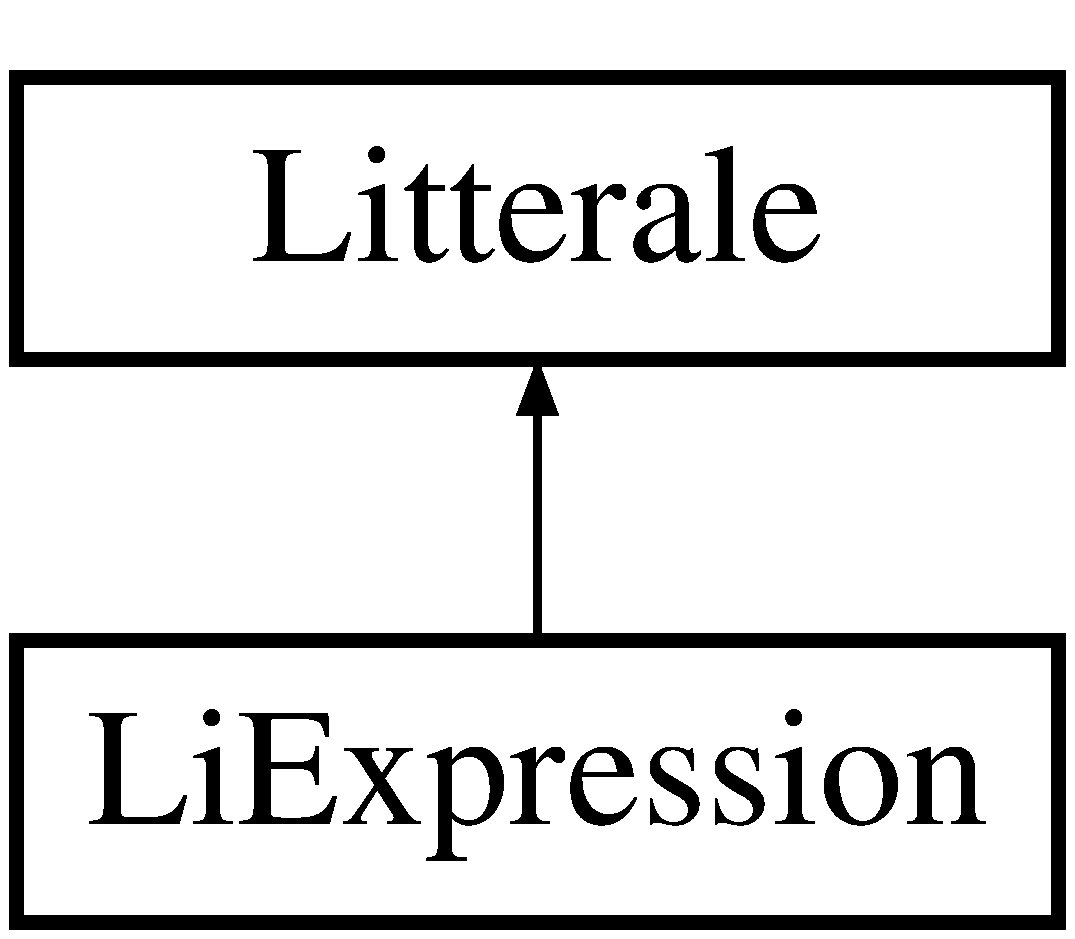
\includegraphics[height=2.000000cm]{class_li_expression}
\end{center}
\end{figure}
\subsection*{Public Member Functions}
\begin{DoxyCompactItemize}
\item 
\hyperlink{class_li_expression_a33617047988cf710ee800aa463485e27}{Li\+Expression} (Q\+String a)
\begin{DoxyCompactList}\small\item\em Constructor. \end{DoxyCompactList}\item 
Q\+String \hyperlink{class_li_expression_a0bd7e53567dc458d662a225fbd0d3085}{get\+Expression} () const 
\begin{DoxyCompactList}\small\item\em \hyperlink{class_li_expression_a0bd7e53567dc458d662a225fbd0d3085}{get\+Expression()} method \end{DoxyCompactList}\item 
string \hyperlink{class_li_expression_afbf36946d48981027d8af7685c950a9b}{to\+String} () const 
\begin{DoxyCompactList}\small\item\em \hyperlink{class_li_expression_afbf36946d48981027d8af7685c950a9b}{to\+String()} method \end{DoxyCompactList}\item 
bool \hyperlink{class_li_expression_ac6e982f0986c28b01a1221830bce20eb}{is\+Zero} () const 
\begin{DoxyCompactList}\small\item\em \hyperlink{class_li_expression_ac6e982f0986c28b01a1221830bce20eb}{is\+Zero()} method \end{DoxyCompactList}\item 
int \hyperlink{class_li_expression_a17e0a77c27727e85d3784527c217827e}{get\+Value} () const 
\begin{DoxyCompactList}\small\item\em \hyperlink{class_li_expression_a17e0a77c27727e85d3784527c217827e}{get\+Value()} method \end{DoxyCompactList}\item 
int \hyperlink{class_li_expression_a5a4547ae8674412134264a8cd436e938}{get\+Numerateur} () const 
\begin{DoxyCompactList}\small\item\em get\+Numerator() method \end{DoxyCompactList}\item 
int \hyperlink{class_li_expression_ab0c4fc0767e78b313d2ac4741bc9a8e7}{get\+Denominateur} () const 
\begin{DoxyCompactList}\small\item\em get\+Denominator() method \end{DoxyCompactList}\item 
double \hyperlink{class_li_expression_a6810603f331aa6a054df4e4d9f64ba4a}{get\+Reel} () const 
\begin{DoxyCompactList}\small\item\em \hyperlink{class_li_expression_a6810603f331aa6a054df4e4d9f64ba4a}{get\+Reel()} method \end{DoxyCompactList}\item 
\hyperlink{class_litterale}{Litterale} $\ast$ \hyperlink{class_li_expression_aba0fbbab32512bad7e67aa23d2e50318}{operator+} (const \hyperlink{class_litterale}{Litterale} \&li) const 
\begin{DoxyCompactList}\small\item\em operator+ \end{DoxyCompactList}\item 
\hyperlink{class_litterale}{Litterale} $\ast$ \hyperlink{class_li_expression_a459ed09d7f610ff88e606fc95e0b22a5}{operator-\/} (const \hyperlink{class_litterale}{Litterale} \&li) const 
\begin{DoxyCompactList}\small\item\em operator-\/ \end{DoxyCompactList}\item 
\hyperlink{class_litterale}{Litterale} $\ast$ \hyperlink{class_li_expression_a6d6c07034ea7c50301164e27d1af48fc}{operator/} (const \hyperlink{class_litterale}{Litterale} \&li) const 
\begin{DoxyCompactList}\small\item\em operator/ \end{DoxyCompactList}\item 
\hyperlink{class_litterale}{Litterale} $\ast$ \hyperlink{class_li_expression_a14d8c244f1d0a5035781e999220f6972}{operator$\ast$} (const \hyperlink{class_litterale}{Litterale} \&li) const 
\begin{DoxyCompactList}\small\item\em operator$\ast$ \end{DoxyCompactList}\item 
\hyperlink{class_litterale}{Litterale} $\ast$ \hyperlink{class_li_expression_a30334b98ebe99c3b06596b964b74aa2b}{operator==} (const \hyperlink{class_litterale}{Litterale} \&li) const 
\begin{DoxyCompactList}\small\item\em operator== \end{DoxyCompactList}\item 
\hyperlink{class_litterale}{Litterale} $\ast$ \hyperlink{class_li_expression_a109d27f2e3a8717a0cd391db8042f3d7}{operator!=} (const \hyperlink{class_litterale}{Litterale} \&li) const 
\begin{DoxyCompactList}\small\item\em operator!= \end{DoxyCompactList}\item 
\hyperlink{class_litterale}{Litterale} $\ast$ \hyperlink{class_li_expression_a2803c38127ed58e1d8148e06e079dbb4}{operator$<$=} (const \hyperlink{class_litterale}{Litterale} \&li) const 
\begin{DoxyCompactList}\small\item\em operator$<$= \end{DoxyCompactList}\item 
\hyperlink{class_litterale}{Litterale} $\ast$ \hyperlink{class_li_expression_a9559555748722ee6f1a384527fef29a1}{operator$>$=} (const \hyperlink{class_litterale}{Litterale} \&li) const 
\begin{DoxyCompactList}\small\item\em operator$>$= \end{DoxyCompactList}\item 
\hyperlink{class_litterale}{Litterale} $\ast$ \hyperlink{class_li_expression_aa0182e19cd3c065f7da2318fdbd261fe}{operator$<$} (const \hyperlink{class_litterale}{Litterale} \&li) const 
\begin{DoxyCompactList}\small\item\em operator$<$ \end{DoxyCompactList}\item 
\hyperlink{class_litterale}{Litterale} $\ast$ \hyperlink{class_li_expression_a31d73a19962932144004d181dd46a203}{operator$>$} (const \hyperlink{class_litterale}{Litterale} \&li) const 
\begin{DoxyCompactList}\small\item\em operator$>$ \end{DoxyCompactList}\item 
\hyperlink{class_litterale}{Litterale} $\ast$ \hyperlink{class_li_expression_aff040ab50e34119fc3ef87a3810857dd}{Num} ()
\begin{DoxyCompactList}\small\item\em N\+U\+M() method. \end{DoxyCompactList}\item 
\hyperlink{class_litterale}{Litterale} $\ast$ \hyperlink{class_li_expression_ab135c92b3d0378fea00a60f096fab7d6}{Den} ()
\begin{DoxyCompactList}\small\item\em D\+E\+N() method. \end{DoxyCompactList}\item 
\hyperlink{class_litterale}{Litterale} $\ast$ \hyperlink{class_li_expression_ae1a4046463009818bd96794ba65bd6b4}{Re} ()
\begin{DoxyCompactList}\small\item\em R\+E() method. \end{DoxyCompactList}\item 
\hyperlink{class_litterale}{Litterale} $\ast$ \hyperlink{class_li_expression_ac9f9dae0e22ae52c5c8e92a3b4dc6a2a}{Im} ()
\begin{DoxyCompactList}\small\item\em I\+M() method. \end{DoxyCompactList}\item 
\hyperlink{class_litterale}{Litterale} $\ast$ \hyperlink{class_li_expression_a0bf45253ed1ac7d76d0950f5368f634c}{Neg} ()
\begin{DoxyCompactList}\small\item\em N\+E\+G() method. \end{DoxyCompactList}\item 
\hyperlink{class_litterale}{Litterale} $\ast$ \hyperlink{class_li_expression_afc9c8a7d8d16b6b834708daa1c8bb431}{Div} (const \hyperlink{class_litterale}{Litterale} \&li)
\begin{DoxyCompactList}\small\item\em D\+I\+V() method. \end{DoxyCompactList}\item 
\hyperlink{class_litterale}{Litterale} $\ast$ \hyperlink{class_li_expression_adb379aef8c3782698a76bc56d0c6758d}{Mod} (const \hyperlink{class_litterale}{Litterale} \&li)
\begin{DoxyCompactList}\small\item\em M\+O\+D() method. \end{DoxyCompactList}\item 
\hyperlink{class_litterale}{Litterale} $\ast$ \hyperlink{class_li_expression_a6e29f5bd106989a72e8096d3481fd326}{And} (const \hyperlink{class_litterale}{Litterale} $\ast$li)
\begin{DoxyCompactList}\small\item\em A\+N\+D() method. \end{DoxyCompactList}\item 
\hyperlink{class_litterale}{Litterale} $\ast$ \hyperlink{class_li_expression_a12cb399c149c2b5383ec7207bd04ed8a}{Or} (const \hyperlink{class_litterale}{Litterale} $\ast$li)
\begin{DoxyCompactList}\small\item\em O\+R() method. \end{DoxyCompactList}\item 
\hyperlink{class_litterale}{Litterale} $\ast$ \hyperlink{class_li_expression_ac07a8597d82ce267204cb3bbd3c6fba1}{Not} ()
\begin{DoxyCompactList}\small\item\em N\+O\+T() method. \end{DoxyCompactList}\item 
\hyperlink{class_litterale}{Litterale} $\ast$ {\bfseries Clone} () const \hypertarget{class_li_expression_a92141a34e0297771921e620250165580}{}\label{class_li_expression_a92141a34e0297771921e620250165580}

\end{DoxyCompactItemize}
\subsection*{Static Public Member Functions}
\begin{DoxyCompactItemize}
\item 
static \hyperlink{class_li_expression}{Li\+Expression} $\ast$ \hyperlink{class_li_expression_a546296a44c992147e6d9f9c29ea863ec}{enlever\+Guillemets} (const Q\+String \&s)
\begin{DoxyCompactList}\small\item\em \hyperlink{class_li_expression_a546296a44c992147e6d9f9c29ea863ec}{enlever\+Guillemets()} method \end{DoxyCompactList}\end{DoxyCompactItemize}


\subsection{Constructor \& Destructor Documentation}
\index{Li\+Expression@{Li\+Expression}!Li\+Expression@{Li\+Expression}}
\index{Li\+Expression@{Li\+Expression}!Li\+Expression@{Li\+Expression}}
\subsubsection[{\texorpdfstring{Li\+Expression(\+Q\+String a)}{LiExpression(QString a)}}]{\setlength{\rightskip}{0pt plus 5cm}Li\+Expression\+::\+Li\+Expression (
\begin{DoxyParamCaption}
\item[{Q\+String}]{a}
\end{DoxyParamCaption}
)\hspace{0.3cm}{\ttfamily [inline]}}\hypertarget{class_li_expression_a33617047988cf710ee800aa463485e27}{}\label{class_li_expression_a33617047988cf710ee800aa463485e27}


Constructor. 

Constructor of the \hyperlink{class_li_expression}{Li\+Expression} class Inline Method


\begin{DoxyParams}{Parameters}
{\em 1} & parameter of type Q\+String to initialize exp \\
\hline
\end{DoxyParams}


\subsection{Member Function Documentation}
\index{Li\+Expression@{Li\+Expression}!And@{And}}
\index{And@{And}!Li\+Expression@{Li\+Expression}}
\subsubsection[{\texorpdfstring{And(const Litterale $\ast$li)}{And(const Litterale *li)}}]{\setlength{\rightskip}{0pt plus 5cm}{\bf Litterale} $\ast$ Li\+Expression\+::\+And (
\begin{DoxyParamCaption}
\item[{const {\bf Litterale} $\ast$}]{li}
\end{DoxyParamCaption}
)\hspace{0.3cm}{\ttfamily [virtual]}}\hypertarget{class_li_expression_a6e29f5bd106989a72e8096d3481fd326}{}\label{class_li_expression_a6e29f5bd106989a72e8096d3481fd326}


A\+N\+D() method. 

Construct a new Q\+String (concatenation of the operator and the 2 Litterales)


\begin{DoxyParams}{Parameters}
{\em const} & \hyperlink{class_litterale}{Litterale}\& (parameter should not be modified) \\
\hline
\end{DoxyParams}
\begin{DoxyReturn}{Returns}
Litterale$\ast$ 
\end{DoxyReturn}


Implements \hyperlink{class_litterale_a2331619771c5cb74bee253e2c2cf62f5}{Litterale}.

\index{Li\+Expression@{Li\+Expression}!Den@{Den}}
\index{Den@{Den}!Li\+Expression@{Li\+Expression}}
\subsubsection[{\texorpdfstring{Den()}{Den()}}]{\setlength{\rightskip}{0pt plus 5cm}{\bf Litterale} $\ast$ Li\+Expression\+::\+Den (
\begin{DoxyParamCaption}
{}
\end{DoxyParamCaption}
)\hspace{0.3cm}{\ttfamily [virtual]}}\hypertarget{class_li_expression_ab135c92b3d0378fea00a60f096fab7d6}{}\label{class_li_expression_ab135c92b3d0378fea00a60f096fab7d6}


D\+E\+N() method. 

Construct a new Q\+String (concatenation of the operator and the 2 Litterales)


\begin{DoxyParams}{Parameters}
{\em no} & parameter \\
\hline
\end{DoxyParams}
\begin{DoxyReturn}{Returns}
Litterale$\ast$ 
\end{DoxyReturn}


Implements \hyperlink{class_litterale_aedcaa806cc6b037371b25d12086503b8}{Litterale}.

\index{Li\+Expression@{Li\+Expression}!Div@{Div}}
\index{Div@{Div}!Li\+Expression@{Li\+Expression}}
\subsubsection[{\texorpdfstring{Div(const Litterale \&li)}{Div(const Litterale &li)}}]{\setlength{\rightskip}{0pt plus 5cm}{\bf Litterale} $\ast$ Li\+Expression\+::\+Div (
\begin{DoxyParamCaption}
\item[{const {\bf Litterale} \&}]{li}
\end{DoxyParamCaption}
)}\hypertarget{class_li_expression_afc9c8a7d8d16b6b834708daa1c8bb431}{}\label{class_li_expression_afc9c8a7d8d16b6b834708daa1c8bb431}


D\+I\+V() method. 

Construct a new Q\+String (concatenation of the operator and the 2 Litterales)


\begin{DoxyParams}{Parameters}
{\em const} & \hyperlink{class_litterale}{Litterale}\& (parameter should not be modified) \\
\hline
\end{DoxyParams}
\begin{DoxyReturn}{Returns}
Litterale$\ast$ 
\end{DoxyReturn}
\index{Li\+Expression@{Li\+Expression}!enlever\+Guillemets@{enlever\+Guillemets}}
\index{enlever\+Guillemets@{enlever\+Guillemets}!Li\+Expression@{Li\+Expression}}
\subsubsection[{\texorpdfstring{enlever\+Guillemets(const Q\+String \&s)}{enleverGuillemets(const QString &s)}}]{\setlength{\rightskip}{0pt plus 5cm}{\bf Li\+Expression} $\ast$ Li\+Expression\+::enlever\+Guillemets (
\begin{DoxyParamCaption}
\item[{const Q\+String \&}]{s}
\end{DoxyParamCaption}
)\hspace{0.3cm}{\ttfamily [static]}}\hypertarget{class_li_expression_a546296a44c992147e6d9f9c29ea863ec}{}\label{class_li_expression_a546296a44c992147e6d9f9c29ea863ec}


\hyperlink{class_li_expression_a546296a44c992147e6d9f9c29ea863ec}{enlever\+Guillemets()} method 

Static method (it will be needed in other classes) Used to detached the quotation marks When a user wants to put an expression into the calculator, he has to put it between quotations marks Then the expression will be evaluated


\begin{DoxyParams}{Parameters}
{\em const} & Q\+String\& \\
\hline
\end{DoxyParams}
\begin{DoxyReturn}{Returns}
pointer to \hyperlink{class_li_expression}{Li\+Expression} 
\end{DoxyReturn}
\index{Li\+Expression@{Li\+Expression}!get\+Denominateur@{get\+Denominateur}}
\index{get\+Denominateur@{get\+Denominateur}!Li\+Expression@{Li\+Expression}}
\subsubsection[{\texorpdfstring{get\+Denominateur() const }{getDenominateur() const }}]{\setlength{\rightskip}{0pt plus 5cm}int Li\+Expression\+::get\+Denominateur (
\begin{DoxyParamCaption}
{}
\end{DoxyParamCaption}
) const\hspace{0.3cm}{\ttfamily [inline]}, {\ttfamily [virtual]}}\hypertarget{class_li_expression_ab0c4fc0767e78b313d2ac4741bc9a8e7}{}\label{class_li_expression_ab0c4fc0767e78b313d2ac4741bc9a8e7}


get\+Denominator() method 

Accessor of the \hyperlink{class_li_rationnelle}{Li\+Rationnelle} class (pure virtual in the \hyperlink{class_litterale}{Litterale} class) Throws a \hyperlink{class_li_exception}{Li\+Exception} (can only be called on \hyperlink{class_li_rationnelle}{Li\+Rationnelle})


\begin{DoxyParams}{Parameters}
{\em no} & parameter \\
\hline
\end{DoxyParams}
\begin{DoxyReturn}{Returns}
int 
\end{DoxyReturn}


Reimplemented from \hyperlink{class_litterale_a68a07beac9e8a4e71d3920a4c6c27cc7}{Litterale}.

\index{Li\+Expression@{Li\+Expression}!get\+Expression@{get\+Expression}}
\index{get\+Expression@{get\+Expression}!Li\+Expression@{Li\+Expression}}
\subsubsection[{\texorpdfstring{get\+Expression() const }{getExpression() const }}]{\setlength{\rightskip}{0pt plus 5cm}Q\+String Li\+Expression\+::get\+Expression (
\begin{DoxyParamCaption}
{}
\end{DoxyParamCaption}
) const\hspace{0.3cm}{\ttfamily [inline]}}\hypertarget{class_li_expression_a0bd7e53567dc458d662a225fbd0d3085}{}\label{class_li_expression_a0bd7e53567dc458d662a225fbd0d3085}


\hyperlink{class_li_expression_a0bd7e53567dc458d662a225fbd0d3085}{get\+Expression()} method 

Accessor to the attribute of a \hyperlink{class_li_expression}{Li\+Expression} object


\begin{DoxyParams}{Parameters}
{\em no} & parameter \\
\hline
\end{DoxyParams}
\begin{DoxyReturn}{Returns}
Q\+String 
\end{DoxyReturn}
\index{Li\+Expression@{Li\+Expression}!get\+Numerateur@{get\+Numerateur}}
\index{get\+Numerateur@{get\+Numerateur}!Li\+Expression@{Li\+Expression}}
\subsubsection[{\texorpdfstring{get\+Numerateur() const }{getNumerateur() const }}]{\setlength{\rightskip}{0pt plus 5cm}int Li\+Expression\+::get\+Numerateur (
\begin{DoxyParamCaption}
{}
\end{DoxyParamCaption}
) const\hspace{0.3cm}{\ttfamily [inline]}, {\ttfamily [virtual]}}\hypertarget{class_li_expression_a5a4547ae8674412134264a8cd436e938}{}\label{class_li_expression_a5a4547ae8674412134264a8cd436e938}


get\+Numerator() method 

Accessor of the \hyperlink{class_li_rationnelle}{Li\+Rationnelle} class (pure virtual in the \hyperlink{class_litterale}{Litterale} class) Throws a \hyperlink{class_li_exception}{Li\+Exception} (can only be called on \hyperlink{class_li_rationnelle}{Li\+Rationnelle})


\begin{DoxyParams}{Parameters}
{\em no} & parameter \\
\hline
\end{DoxyParams}
\begin{DoxyReturn}{Returns}
int 
\end{DoxyReturn}


Reimplemented from \hyperlink{class_litterale_a6d3e582118775a3a0362154ae1a8cbda}{Litterale}.

\index{Li\+Expression@{Li\+Expression}!get\+Reel@{get\+Reel}}
\index{get\+Reel@{get\+Reel}!Li\+Expression@{Li\+Expression}}
\subsubsection[{\texorpdfstring{get\+Reel() const }{getReel() const }}]{\setlength{\rightskip}{0pt plus 5cm}double Li\+Expression\+::get\+Reel (
\begin{DoxyParamCaption}
{}
\end{DoxyParamCaption}
) const\hspace{0.3cm}{\ttfamily [inline]}, {\ttfamily [virtual]}}\hypertarget{class_li_expression_a6810603f331aa6a054df4e4d9f64ba4a}{}\label{class_li_expression_a6810603f331aa6a054df4e4d9f64ba4a}


\hyperlink{class_li_expression_a6810603f331aa6a054df4e4d9f64ba4a}{get\+Reel()} method 

Accessor of the \hyperlink{class_li_reelle}{Li\+Reelle} class (pure virtual in the \hyperlink{class_litterale}{Litterale} class) Throws a \hyperlink{class_li_exception}{Li\+Exception} (can only be called on \hyperlink{class_li_rationnelle}{Li\+Rationnelle})


\begin{DoxyParams}{Parameters}
{\em no} & parameter \\
\hline
\end{DoxyParams}
\begin{DoxyReturn}{Returns}
double 
\end{DoxyReturn}


Reimplemented from \hyperlink{class_litterale_aca56aad5f1a4a691337142e3f5a3b93d}{Litterale}.

\index{Li\+Expression@{Li\+Expression}!get\+Value@{get\+Value}}
\index{get\+Value@{get\+Value}!Li\+Expression@{Li\+Expression}}
\subsubsection[{\texorpdfstring{get\+Value() const }{getValue() const }}]{\setlength{\rightskip}{0pt plus 5cm}int Li\+Expression\+::get\+Value (
\begin{DoxyParamCaption}
{}
\end{DoxyParamCaption}
) const\hspace{0.3cm}{\ttfamily [inline]}, {\ttfamily [virtual]}}\hypertarget{class_li_expression_a17e0a77c27727e85d3784527c217827e}{}\label{class_li_expression_a17e0a77c27727e85d3784527c217827e}


\hyperlink{class_li_expression_a17e0a77c27727e85d3784527c217827e}{get\+Value()} method 

Accessor of the \hyperlink{class_li_entiere}{Li\+Entiere} class (pure virtual in the \hyperlink{class_litterale}{Litterale} class) Throws a \hyperlink{class_li_exception}{Li\+Exception} (can only be called on \hyperlink{class_li_entiere}{Li\+Entiere})


\begin{DoxyParams}{Parameters}
{\em no} & parameter \\
\hline
\end{DoxyParams}
\begin{DoxyReturn}{Returns}
int 
\end{DoxyReturn}


Reimplemented from \hyperlink{class_litterale_a9cd3d639341cb797bcf2b6400d6ad43d}{Litterale}.

\index{Li\+Expression@{Li\+Expression}!Im@{Im}}
\index{Im@{Im}!Li\+Expression@{Li\+Expression}}
\subsubsection[{\texorpdfstring{Im()}{Im()}}]{\setlength{\rightskip}{0pt plus 5cm}{\bf Litterale} $\ast$ Li\+Expression\+::\+Im (
\begin{DoxyParamCaption}
{}
\end{DoxyParamCaption}
)\hspace{0.3cm}{\ttfamily [virtual]}}\hypertarget{class_li_expression_ac9f9dae0e22ae52c5c8e92a3b4dc6a2a}{}\label{class_li_expression_ac9f9dae0e22ae52c5c8e92a3b4dc6a2a}


I\+M() method. 

Construct a new Q\+String (concatenation of the operator and the 2 Litterales)


\begin{DoxyParams}{Parameters}
{\em no} & parameter \\
\hline
\end{DoxyParams}
\begin{DoxyReturn}{Returns}
Litterale$\ast$ 
\end{DoxyReturn}


Implements \hyperlink{class_litterale_a8f0c2d98186c545f4f34ae07b9751f97}{Litterale}.

\index{Li\+Expression@{Li\+Expression}!is\+Zero@{is\+Zero}}
\index{is\+Zero@{is\+Zero}!Li\+Expression@{Li\+Expression}}
\subsubsection[{\texorpdfstring{is\+Zero() const }{isZero() const }}]{\setlength{\rightskip}{0pt plus 5cm}bool Li\+Expression\+::is\+Zero (
\begin{DoxyParamCaption}
{}
\end{DoxyParamCaption}
) const\hspace{0.3cm}{\ttfamily [inline]}, {\ttfamily [virtual]}}\hypertarget{class_li_expression_ac6e982f0986c28b01a1221830bce20eb}{}\label{class_li_expression_ac6e982f0986c28b01a1221830bce20eb}


\hyperlink{class_li_expression_ac6e982f0986c28b01a1221830bce20eb}{is\+Zero()} method 

Used to inform us if the attribut is empty or not. This method was pure virtual in \hyperlink{class_litterale}{Litterale} Inline Method


\begin{DoxyParams}{Parameters}
{\em no} & parameter \\
\hline
\end{DoxyParams}
\begin{DoxyReturn}{Returns}
bool 
\end{DoxyReturn}


Implements \hyperlink{class_litterale_a535fc431d96954754b7a729404df4a79}{Litterale}.

\index{Li\+Expression@{Li\+Expression}!Mod@{Mod}}
\index{Mod@{Mod}!Li\+Expression@{Li\+Expression}}
\subsubsection[{\texorpdfstring{Mod(const Litterale \&li)}{Mod(const Litterale &li)}}]{\setlength{\rightskip}{0pt plus 5cm}{\bf Litterale} $\ast$ Li\+Expression\+::\+Mod (
\begin{DoxyParamCaption}
\item[{const {\bf Litterale} \&}]{li}
\end{DoxyParamCaption}
)}\hypertarget{class_li_expression_adb379aef8c3782698a76bc56d0c6758d}{}\label{class_li_expression_adb379aef8c3782698a76bc56d0c6758d}


M\+O\+D() method. 

Construct a new Q\+String (concatenation of the operator and the 2 Litterales)


\begin{DoxyParams}{Parameters}
{\em const} & \hyperlink{class_litterale}{Litterale}\& (parameter should not be modified) \\
\hline
\end{DoxyParams}
\begin{DoxyReturn}{Returns}
Litterale$\ast$ 
\end{DoxyReturn}
\index{Li\+Expression@{Li\+Expression}!Neg@{Neg}}
\index{Neg@{Neg}!Li\+Expression@{Li\+Expression}}
\subsubsection[{\texorpdfstring{Neg()}{Neg()}}]{\setlength{\rightskip}{0pt plus 5cm}{\bf Litterale} $\ast$ Li\+Expression\+::\+Neg (
\begin{DoxyParamCaption}
{}
\end{DoxyParamCaption}
)\hspace{0.3cm}{\ttfamily [virtual]}}\hypertarget{class_li_expression_a0bf45253ed1ac7d76d0950f5368f634c}{}\label{class_li_expression_a0bf45253ed1ac7d76d0950f5368f634c}


N\+E\+G() method. 

Construct a new Q\+String (concatenation of the operator and the 2 Litterales)


\begin{DoxyParams}{Parameters}
{\em no} & parameter \\
\hline
\end{DoxyParams}
\begin{DoxyReturn}{Returns}
Litterale$\ast$ 
\end{DoxyReturn}


Implements \hyperlink{class_litterale_ac9261e971a9d7d84137557d1cad94336}{Litterale}.

\index{Li\+Expression@{Li\+Expression}!Not@{Not}}
\index{Not@{Not}!Li\+Expression@{Li\+Expression}}
\subsubsection[{\texorpdfstring{Not()}{Not()}}]{\setlength{\rightskip}{0pt plus 5cm}{\bf Litterale} $\ast$ Li\+Expression\+::\+Not (
\begin{DoxyParamCaption}
{}
\end{DoxyParamCaption}
)\hspace{0.3cm}{\ttfamily [virtual]}}\hypertarget{class_li_expression_ac07a8597d82ce267204cb3bbd3c6fba1}{}\label{class_li_expression_ac07a8597d82ce267204cb3bbd3c6fba1}


N\+O\+T() method. 

Construct a new Q\+String (concatenation of the operator and the 2 Litterales)


\begin{DoxyParams}{Parameters}
{\em const} & \hyperlink{class_litterale}{Litterale}\& (parameter should not be modified) \\
\hline
\end{DoxyParams}
\begin{DoxyReturn}{Returns}
Litterale$\ast$ 
\end{DoxyReturn}


Implements \hyperlink{class_litterale_af44ae987ec5db62170efb3aec563c95c}{Litterale}.

\index{Li\+Expression@{Li\+Expression}!Num@{Num}}
\index{Num@{Num}!Li\+Expression@{Li\+Expression}}
\subsubsection[{\texorpdfstring{Num()}{Num()}}]{\setlength{\rightskip}{0pt plus 5cm}{\bf Litterale} $\ast$ Li\+Expression\+::\+Num (
\begin{DoxyParamCaption}
{}
\end{DoxyParamCaption}
)\hspace{0.3cm}{\ttfamily [virtual]}}\hypertarget{class_li_expression_aff040ab50e34119fc3ef87a3810857dd}{}\label{class_li_expression_aff040ab50e34119fc3ef87a3810857dd}


N\+U\+M() method. 

Construct a new Q\+String (concatenation of the operator and the 2 Litterales)


\begin{DoxyParams}{Parameters}
{\em no} & parameter \\
\hline
\end{DoxyParams}
\begin{DoxyReturn}{Returns}
Litterale$\ast$ 
\end{DoxyReturn}


Implements \hyperlink{class_litterale_a4f02faabce1e1f46c4d34508de316a2b}{Litterale}.

\index{Li\+Expression@{Li\+Expression}!operator"!=@{operator"!=}}
\index{operator"!=@{operator"!=}!Li\+Expression@{Li\+Expression}}
\subsubsection[{\texorpdfstring{operator"!=(const Litterale \&li) const }{operator!=(const Litterale &li) const }}]{\setlength{\rightskip}{0pt plus 5cm}{\bf Litterale}$\ast$ Li\+Expression\+::operator!= (
\begin{DoxyParamCaption}
\item[{const {\bf Litterale} \&}]{li}
\end{DoxyParamCaption}
) const\hspace{0.3cm}{\ttfamily [inline]}, {\ttfamily [virtual]}}\hypertarget{class_li_expression_a109d27f2e3a8717a0cd391db8042f3d7}{}\label{class_li_expression_a109d27f2e3a8717a0cd391db8042f3d7}


operator!= 

Overloaded operator!= Throws a \hyperlink{class_li_exception}{Li\+Exception} (can not compare a \hyperlink{class_litterale}{Litterale} and a \hyperlink{class_li_expression}{Li\+Expression})


\begin{DoxyParams}{Parameters}
{\em const} & \hyperlink{class_litterale}{Litterale}\& \\
\hline
\end{DoxyParams}
\begin{DoxyReturn}{Returns}
Litterale$\ast$ 
\end{DoxyReturn}


Implements \hyperlink{class_litterale_aec92913de9d127360897b0d644b5a44f}{Litterale}.

\index{Li\+Expression@{Li\+Expression}!operator$\ast$@{operator$\ast$}}
\index{operator$\ast$@{operator$\ast$}!Li\+Expression@{Li\+Expression}}
\subsubsection[{\texorpdfstring{operator$\ast$(const Litterale \&li) const }{operator*(const Litterale &li) const }}]{\setlength{\rightskip}{0pt plus 5cm}{\bf Litterale} $\ast$ Li\+Expression\+::operator$\ast$ (
\begin{DoxyParamCaption}
\item[{const {\bf Litterale} \&}]{li}
\end{DoxyParamCaption}
) const\hspace{0.3cm}{\ttfamily [virtual]}}\hypertarget{class_li_expression_a14d8c244f1d0a5035781e999220f6972}{}\label{class_li_expression_a14d8c244f1d0a5035781e999220f6972}


operator$\ast$ 

Overloaded operator$\ast$ const method (attribut should not be modified) Used to multiply a \hyperlink{class_li_expression}{Li\+Expression} and a \hyperlink{class_litterale}{Litterale} Construct a new Q\+String (concatenation of the 2 Litterale$\ast$)


\begin{DoxyParams}{Parameters}
{\em const} & \hyperlink{class_litterale}{Litterale}\& (parameter should not be modified) \\
\hline
\end{DoxyParams}
\begin{DoxyReturn}{Returns}
pointer to \hyperlink{class_litterale}{Litterale} 
\end{DoxyReturn}


Implements \hyperlink{class_litterale_a54eb0d992188da6b490418bdd828b096}{Litterale}.

\index{Li\+Expression@{Li\+Expression}!operator+@{operator+}}
\index{operator+@{operator+}!Li\+Expression@{Li\+Expression}}
\subsubsection[{\texorpdfstring{operator+(const Litterale \&li) const }{operator+(const Litterale &li) const }}]{\setlength{\rightskip}{0pt plus 5cm}{\bf Litterale} $\ast$ Li\+Expression\+::operator+ (
\begin{DoxyParamCaption}
\item[{const {\bf Litterale} \&}]{li}
\end{DoxyParamCaption}
) const\hspace{0.3cm}{\ttfamily [virtual]}}\hypertarget{class_li_expression_aba0fbbab32512bad7e67aa23d2e50318}{}\label{class_li_expression_aba0fbbab32512bad7e67aa23d2e50318}


operator+ 

Overloaded operator+ const method (attribut should not be modified) Used to add a \hyperlink{class_li_expression}{Li\+Expression} and a \hyperlink{class_litterale}{Litterale} Construct a new Q\+String (concatenation of the 2 Litterale$\ast$)


\begin{DoxyParams}{Parameters}
{\em const} & \hyperlink{class_litterale}{Litterale}\& (parameter should not be modified) \\
\hline
\end{DoxyParams}
\begin{DoxyReturn}{Returns}
pointer to \hyperlink{class_litterale}{Litterale} 
\end{DoxyReturn}


Implements \hyperlink{class_litterale_af4f96b09214b34ae26fe3f2722c42cc0}{Litterale}.

\index{Li\+Expression@{Li\+Expression}!operator-\/@{operator-\/}}
\index{operator-\/@{operator-\/}!Li\+Expression@{Li\+Expression}}
\subsubsection[{\texorpdfstring{operator-\/(const Litterale \&li) const }{operator-(const Litterale &li) const }}]{\setlength{\rightskip}{0pt plus 5cm}{\bf Litterale} $\ast$ Li\+Expression\+::operator-\/ (
\begin{DoxyParamCaption}
\item[{const {\bf Litterale} \&}]{li}
\end{DoxyParamCaption}
) const\hspace{0.3cm}{\ttfamily [virtual]}}\hypertarget{class_li_expression_a459ed09d7f610ff88e606fc95e0b22a5}{}\label{class_li_expression_a459ed09d7f610ff88e606fc95e0b22a5}


operator-\/ 

Overloaded operator-\/ const method (attribut should not be modified) Used to substract to a \hyperlink{class_li_expression}{Li\+Expression} a \hyperlink{class_litterale}{Litterale} Construct a new Q\+String (concatenation of the 2 Litterale$\ast$)


\begin{DoxyParams}{Parameters}
{\em const} & \hyperlink{class_litterale}{Litterale}\& (parameter should not be modified) \\
\hline
\end{DoxyParams}
\begin{DoxyReturn}{Returns}
pointer to \hyperlink{class_litterale}{Litterale} 
\end{DoxyReturn}


Implements \hyperlink{class_litterale_a52eec71121af9c4bbf30011eccc87a68}{Litterale}.

\index{Li\+Expression@{Li\+Expression}!operator/@{operator/}}
\index{operator/@{operator/}!Li\+Expression@{Li\+Expression}}
\subsubsection[{\texorpdfstring{operator/(const Litterale \&li) const }{operator/(const Litterale &li) const }}]{\setlength{\rightskip}{0pt plus 5cm}{\bf Litterale} $\ast$ Li\+Expression\+::operator/ (
\begin{DoxyParamCaption}
\item[{const {\bf Litterale} \&}]{li}
\end{DoxyParamCaption}
) const\hspace{0.3cm}{\ttfamily [virtual]}}\hypertarget{class_li_expression_a6d6c07034ea7c50301164e27d1af48fc}{}\label{class_li_expression_a6d6c07034ea7c50301164e27d1af48fc}


operator/ 

Overloaded operator/ const method (attribut should not be modified) Used to divid a \hyperlink{class_li_expression}{Li\+Expression} by a \hyperlink{class_litterale}{Litterale} Construct a new Q\+String (concatenation of the 2 Litterale$\ast$)


\begin{DoxyParams}{Parameters}
{\em const} & \hyperlink{class_litterale}{Litterale}\& (parameter should not be modified) \\
\hline
\end{DoxyParams}
\begin{DoxyReturn}{Returns}
pointer to \hyperlink{class_litterale}{Litterale} 
\end{DoxyReturn}


Implements \hyperlink{class_litterale_a91da4f609054b3146007291d199e1f33}{Litterale}.

\index{Li\+Expression@{Li\+Expression}!operator$<$@{operator$<$}}
\index{operator$<$@{operator$<$}!Li\+Expression@{Li\+Expression}}
\subsubsection[{\texorpdfstring{operator$<$(const Litterale \&li) const }{operator<(const Litterale &li) const }}]{\setlength{\rightskip}{0pt plus 5cm}{\bf Litterale}$\ast$ Li\+Expression\+::operator$<$ (
\begin{DoxyParamCaption}
\item[{const {\bf Litterale} \&}]{li}
\end{DoxyParamCaption}
) const\hspace{0.3cm}{\ttfamily [inline]}, {\ttfamily [virtual]}}\hypertarget{class_li_expression_aa0182e19cd3c065f7da2318fdbd261fe}{}\label{class_li_expression_aa0182e19cd3c065f7da2318fdbd261fe}


operator$<$ 

Overloaded operator$>$ Throws a \hyperlink{class_li_exception}{Li\+Exception} (can not compare a \hyperlink{class_litterale}{Litterale} and a \hyperlink{class_li_expression}{Li\+Expression})


\begin{DoxyParams}{Parameters}
{\em const} & \hyperlink{class_litterale}{Litterale}\& \\
\hline
\end{DoxyParams}
\begin{DoxyReturn}{Returns}
Litterale$\ast$ 
\end{DoxyReturn}


Implements \hyperlink{class_litterale_a43ba11f1f3ee6cbf21cd2432708938f9}{Litterale}.

\index{Li\+Expression@{Li\+Expression}!operator$<$=@{operator$<$=}}
\index{operator$<$=@{operator$<$=}!Li\+Expression@{Li\+Expression}}
\subsubsection[{\texorpdfstring{operator$<$=(const Litterale \&li) const }{operator<=(const Litterale &li) const }}]{\setlength{\rightskip}{0pt plus 5cm}{\bf Litterale}$\ast$ Li\+Expression\+::operator$<$= (
\begin{DoxyParamCaption}
\item[{const {\bf Litterale} \&}]{li}
\end{DoxyParamCaption}
) const\hspace{0.3cm}{\ttfamily [inline]}, {\ttfamily [virtual]}}\hypertarget{class_li_expression_a2803c38127ed58e1d8148e06e079dbb4}{}\label{class_li_expression_a2803c38127ed58e1d8148e06e079dbb4}


operator$<$= 

Overloaded operator$<$= Throws a \hyperlink{class_li_exception}{Li\+Exception} (can not compare a \hyperlink{class_litterale}{Litterale} and a \hyperlink{class_li_expression}{Li\+Expression})


\begin{DoxyParams}{Parameters}
{\em const} & \hyperlink{class_litterale}{Litterale}\& \\
\hline
\end{DoxyParams}
\begin{DoxyReturn}{Returns}
Litterale$\ast$ 
\end{DoxyReturn}


Implements \hyperlink{class_litterale_af70f373b306808959e234a366de8d799}{Litterale}.

\index{Li\+Expression@{Li\+Expression}!operator==@{operator==}}
\index{operator==@{operator==}!Li\+Expression@{Li\+Expression}}
\subsubsection[{\texorpdfstring{operator==(const Litterale \&li) const }{operator==(const Litterale &li) const }}]{\setlength{\rightskip}{0pt plus 5cm}{\bf Litterale}$\ast$ Li\+Expression\+::operator== (
\begin{DoxyParamCaption}
\item[{const {\bf Litterale} \&}]{li}
\end{DoxyParamCaption}
) const\hspace{0.3cm}{\ttfamily [inline]}, {\ttfamily [virtual]}}\hypertarget{class_li_expression_a30334b98ebe99c3b06596b964b74aa2b}{}\label{class_li_expression_a30334b98ebe99c3b06596b964b74aa2b}


operator== 

Overloaded operator== Throws a \hyperlink{class_li_exception}{Li\+Exception} (can not compare a \hyperlink{class_litterale}{Litterale} and a \hyperlink{class_li_expression}{Li\+Expression})


\begin{DoxyParams}{Parameters}
{\em const} & \hyperlink{class_litterale}{Litterale}\& \\
\hline
\end{DoxyParams}
\begin{DoxyReturn}{Returns}
Litterale$\ast$ 
\end{DoxyReturn}


Implements \hyperlink{class_litterale_a3d4832d994a32a36cb88f8a7d021b280}{Litterale}.

\index{Li\+Expression@{Li\+Expression}!operator$>$@{operator$>$}}
\index{operator$>$@{operator$>$}!Li\+Expression@{Li\+Expression}}
\subsubsection[{\texorpdfstring{operator$>$(const Litterale \&li) const }{operator>(const Litterale &li) const }}]{\setlength{\rightskip}{0pt plus 5cm}{\bf Litterale}$\ast$ Li\+Expression\+::operator$>$ (
\begin{DoxyParamCaption}
\item[{const {\bf Litterale} \&}]{li}
\end{DoxyParamCaption}
) const\hspace{0.3cm}{\ttfamily [inline]}, {\ttfamily [virtual]}}\hypertarget{class_li_expression_a31d73a19962932144004d181dd46a203}{}\label{class_li_expression_a31d73a19962932144004d181dd46a203}


operator$>$ 

Overloaded operator$>$ Throws a \hyperlink{class_li_exception}{Li\+Exception} (can not compare a \hyperlink{class_litterale}{Litterale} and a \hyperlink{class_li_expression}{Li\+Expression})


\begin{DoxyParams}{Parameters}
{\em const} & \hyperlink{class_litterale}{Litterale}\& \\
\hline
\end{DoxyParams}
\begin{DoxyReturn}{Returns}
Litterale$\ast$ 
\end{DoxyReturn}


Implements \hyperlink{class_litterale_a743719ab28de43c55449a90ccd55a95a}{Litterale}.

\index{Li\+Expression@{Li\+Expression}!operator$>$=@{operator$>$=}}
\index{operator$>$=@{operator$>$=}!Li\+Expression@{Li\+Expression}}
\subsubsection[{\texorpdfstring{operator$>$=(const Litterale \&li) const }{operator>=(const Litterale &li) const }}]{\setlength{\rightskip}{0pt plus 5cm}{\bf Litterale}$\ast$ Li\+Expression\+::operator$>$= (
\begin{DoxyParamCaption}
\item[{const {\bf Litterale} \&}]{li}
\end{DoxyParamCaption}
) const\hspace{0.3cm}{\ttfamily [inline]}, {\ttfamily [virtual]}}\hypertarget{class_li_expression_a9559555748722ee6f1a384527fef29a1}{}\label{class_li_expression_a9559555748722ee6f1a384527fef29a1}


operator$>$= 

Overloaded operator$>$= Throws a \hyperlink{class_li_exception}{Li\+Exception} (can not compare a \hyperlink{class_litterale}{Litterale} and a \hyperlink{class_li_expression}{Li\+Expression})


\begin{DoxyParams}{Parameters}
{\em const} & \hyperlink{class_litterale}{Litterale}\& \\
\hline
\end{DoxyParams}
\begin{DoxyReturn}{Returns}
Litterale$\ast$ 
\end{DoxyReturn}


Implements \hyperlink{class_litterale_af31c8ca0ecaccbc05718193d8858bc5d}{Litterale}.

\index{Li\+Expression@{Li\+Expression}!Or@{Or}}
\index{Or@{Or}!Li\+Expression@{Li\+Expression}}
\subsubsection[{\texorpdfstring{Or(const Litterale $\ast$li)}{Or(const Litterale *li)}}]{\setlength{\rightskip}{0pt plus 5cm}{\bf Litterale} $\ast$ Li\+Expression\+::\+Or (
\begin{DoxyParamCaption}
\item[{const {\bf Litterale} $\ast$}]{li}
\end{DoxyParamCaption}
)\hspace{0.3cm}{\ttfamily [virtual]}}\hypertarget{class_li_expression_a12cb399c149c2b5383ec7207bd04ed8a}{}\label{class_li_expression_a12cb399c149c2b5383ec7207bd04ed8a}


O\+R() method. 

Construct a new Q\+String (concatenation of the operator and the 2 Litterales)


\begin{DoxyParams}{Parameters}
{\em const} & \hyperlink{class_litterale}{Litterale}\& (parameter should not be modified) \\
\hline
\end{DoxyParams}
\begin{DoxyReturn}{Returns}
Litterale$\ast$ 
\end{DoxyReturn}


Implements \hyperlink{class_litterale_a326ce76a35c3d29ad409c9491d5169a1}{Litterale}.

\index{Li\+Expression@{Li\+Expression}!Re@{Re}}
\index{Re@{Re}!Li\+Expression@{Li\+Expression}}
\subsubsection[{\texorpdfstring{Re()}{Re()}}]{\setlength{\rightskip}{0pt plus 5cm}{\bf Litterale} $\ast$ Li\+Expression\+::\+Re (
\begin{DoxyParamCaption}
{}
\end{DoxyParamCaption}
)\hspace{0.3cm}{\ttfamily [virtual]}}\hypertarget{class_li_expression_ae1a4046463009818bd96794ba65bd6b4}{}\label{class_li_expression_ae1a4046463009818bd96794ba65bd6b4}


R\+E() method. 

Construct a new Q\+String (concatenation of the operator and the 2 Litterales)


\begin{DoxyParams}{Parameters}
{\em no} & parameter \\
\hline
\end{DoxyParams}
\begin{DoxyReturn}{Returns}
Litterale$\ast$ 
\end{DoxyReturn}


Implements \hyperlink{class_litterale_ac3ab556147c54f260be336fb53ecb52e}{Litterale}.

\index{Li\+Expression@{Li\+Expression}!to\+String@{to\+String}}
\index{to\+String@{to\+String}!Li\+Expression@{Li\+Expression}}
\subsubsection[{\texorpdfstring{to\+String() const }{toString() const }}]{\setlength{\rightskip}{0pt plus 5cm}string Li\+Expression\+::to\+String (
\begin{DoxyParamCaption}
{}
\end{DoxyParamCaption}
) const\hspace{0.3cm}{\ttfamily [inline]}, {\ttfamily [virtual]}}\hypertarget{class_li_expression_afbf36946d48981027d8af7685c950a9b}{}\label{class_li_expression_afbf36946d48981027d8af7685c950a9b}


\hyperlink{class_li_expression_afbf36946d48981027d8af7685c950a9b}{to\+String()} method 

Used to transform the attribute of type Q\+String into a string This method was pure virtual in \hyperlink{class_litterale}{Litterale} Inline Method


\begin{DoxyParams}{Parameters}
{\em no} & parameter \\
\hline
\end{DoxyParams}
\begin{DoxyReturn}{Returns}
string 
\end{DoxyReturn}


Implements \hyperlink{class_litterale_a3041839e5494df2c93bff2c5cb83ce1f}{Litterale}.



The documentation for this class was generated from the following files\+:\begin{DoxyCompactItemize}
\item 
\hyperlink{liexpression_8h}{liexpression.\+h}\item 
\hyperlink{liexpression_8cpp}{liexpression.\+cpp}\end{DoxyCompactItemize}

\hypertarget{class_li_numerique}{}\section{Li\+Numerique Class Reference}
\label{class_li_numerique}\index{Li\+Numerique@{Li\+Numerique}}
Inheritance diagram for Li\+Numerique\+:\begin{figure}[H]
\begin{center}
\leavevmode
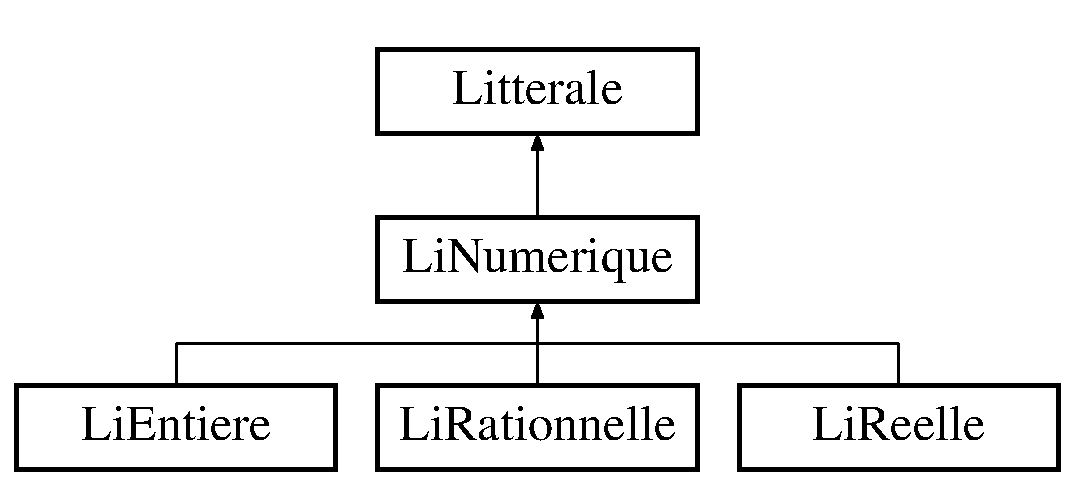
\includegraphics[height=3.000000cm]{class_li_numerique}
\end{center}
\end{figure}
\subsection*{Public Member Functions}
\begin{DoxyCompactItemize}
\item 
virtual string \hyperlink{class_li_numerique_ad40fe29de93bcf18cc2cd088abcb728b}{to\+String} () const  =0
\begin{DoxyCompactList}\small\item\em \hyperlink{class_li_numerique_ad40fe29de93bcf18cc2cd088abcb728b}{to\+String()} method \end{DoxyCompactList}\item 
virtual \hyperlink{class_litterale}{Litterale} $\ast$ {\bfseries Clone} () const  =0\hypertarget{class_li_numerique_af0cd74adc7cc7d970f9d07d7356a1fbd}{}\label{class_li_numerique_af0cd74adc7cc7d970f9d07d7356a1fbd}

\end{DoxyCompactItemize}


\subsection{Member Function Documentation}
\index{Li\+Numerique@{Li\+Numerique}!to\+String@{to\+String}}
\index{to\+String@{to\+String}!Li\+Numerique@{Li\+Numerique}}
\subsubsection[{\texorpdfstring{to\+String() const  =0}{toString() const  =0}}]{\setlength{\rightskip}{0pt plus 5cm}virtual string Li\+Numerique\+::to\+String (
\begin{DoxyParamCaption}
{}
\end{DoxyParamCaption}
) const\hspace{0.3cm}{\ttfamily [pure virtual]}}\hypertarget{class_li_numerique_ad40fe29de93bcf18cc2cd088abcb728b}{}\label{class_li_numerique_ad40fe29de93bcf18cc2cd088abcb728b}


\hyperlink{class_li_numerique_ad40fe29de93bcf18cc2cd088abcb728b}{to\+String()} method 

Pure virtual method used in the \hyperlink{class_litterale_ae33587fb3c4a929c9ee29d9c6b49aea6}{afficher()} method This method have to be defined in the inherited classes


\begin{DoxyParams}{Parameters}
{\em no} & parameter \\
\hline
\end{DoxyParams}
\begin{DoxyReturn}{Returns}
string 
\end{DoxyReturn}


Implements \hyperlink{class_litterale_a3041839e5494df2c93bff2c5cb83ce1f}{Litterale}.



Implemented in \hyperlink{class_li_reelle_ad78df00afab6b86f6b0ec966f848c872}{Li\+Reelle}, \hyperlink{class_li_rationnelle_a2ef7aa4c19e3433794c251cc61296f58}{Li\+Rationnelle}, and \hyperlink{class_li_entiere_a48fceee2e4f1d481b923ebb28a085baf}{Li\+Entiere}.



The documentation for this class was generated from the following file\+:\begin{DoxyCompactItemize}
\item 
\hyperlink{litterale_8h}{litterale.\+h}\end{DoxyCompactItemize}

\hypertarget{class_li_rationnelle}{}\section{Li\+Rationnelle Class Reference}
\label{class_li_rationnelle}\index{Li\+Rationnelle@{Li\+Rationnelle}}
Inheritance diagram for Li\+Rationnelle\+:\begin{figure}[H]
\begin{center}
\leavevmode
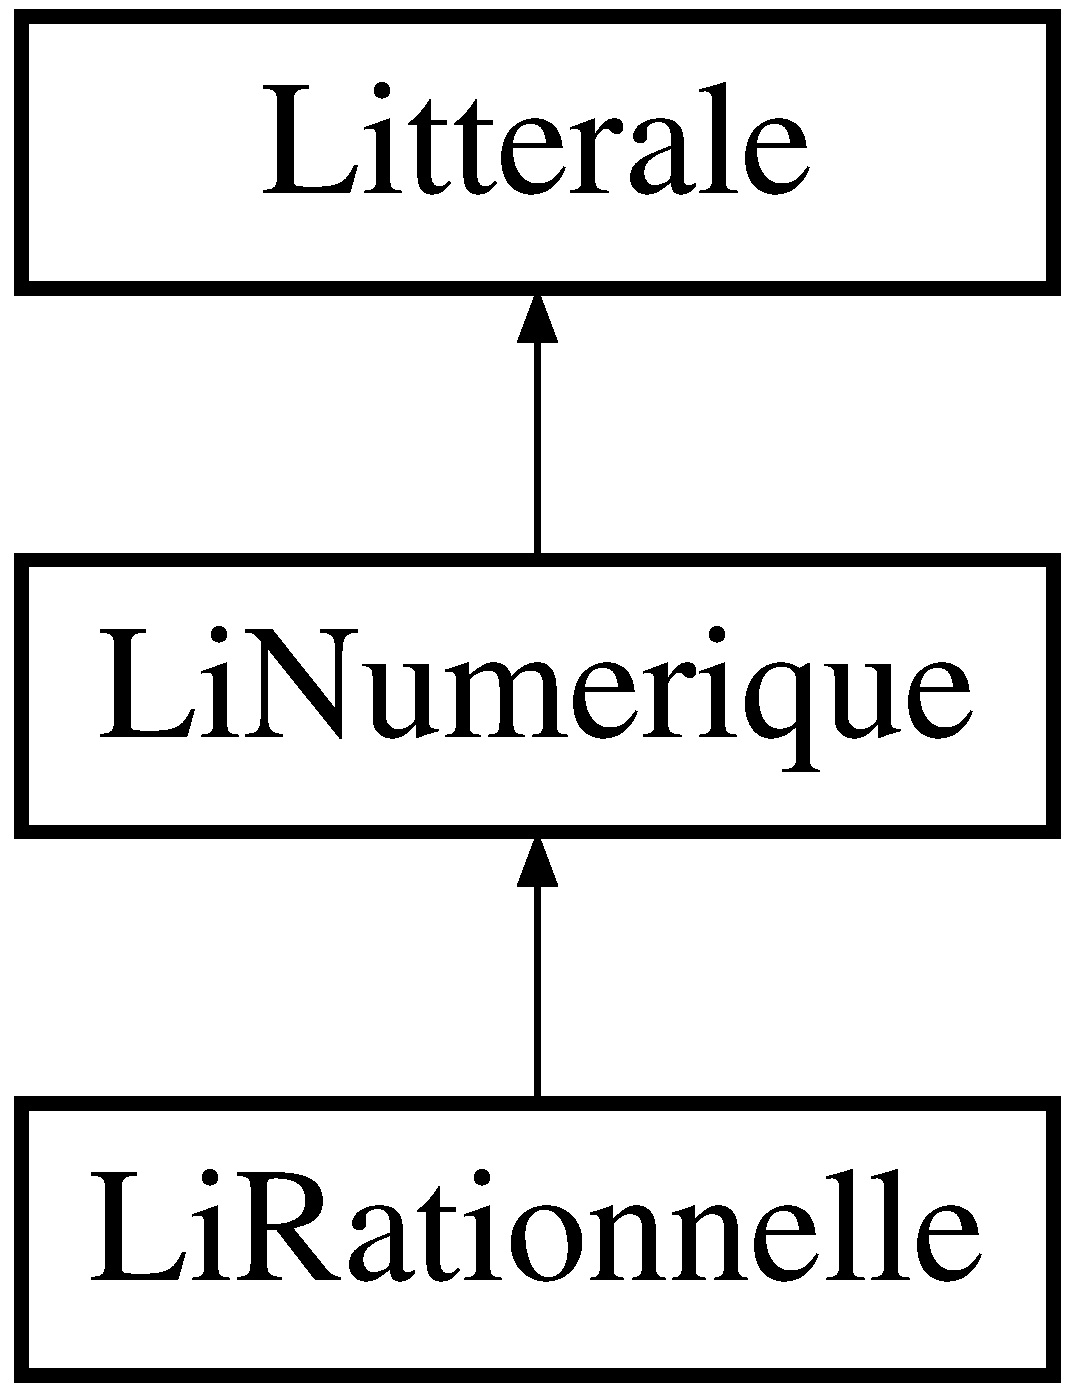
\includegraphics[height=3.000000cm]{class_li_rationnelle}
\end{center}
\end{figure}
\subsection*{Public Member Functions}
\begin{DoxyCompactItemize}
\item 
\hyperlink{class_li_rationnelle_ac88e880e6f08aebfb25e01d8aec740ba}{Li\+Rationnelle} ()
\begin{DoxyCompactList}\small\item\em Constructor. \end{DoxyCompactList}\item 
\hyperlink{class_li_rationnelle_aa8189c481d2f595c7c13ad8e0683cf3c}{Li\+Rationnelle} (int n, int d)
\begin{DoxyCompactList}\small\item\em Constructor. \end{DoxyCompactList}\item 
\hyperlink{class_li_rationnelle_a729eafaf83c01bd5a5d20c0d1cfd7d83}{Li\+Rationnelle} (const \hyperlink{class_li_entiere}{Li\+Entiere} \&n, const \hyperlink{class_li_entiere}{Li\+Entiere} \&d)
\begin{DoxyCompactList}\small\item\em Constructor. \end{DoxyCompactList}\item 
string \hyperlink{class_li_rationnelle_a2ef7aa4c19e3433794c251cc61296f58}{to\+String} () const 
\begin{DoxyCompactList}\small\item\em \hyperlink{class_li_rationnelle_a2ef7aa4c19e3433794c251cc61296f58}{to\+String()} method \end{DoxyCompactList}\item 
void \hyperlink{class_li_rationnelle_a1b96a094c77eb02f6b0728751a10648e}{simplification} ()
\begin{DoxyCompactList}\small\item\em \hyperlink{class_li_rationnelle_a1b96a094c77eb02f6b0728751a10648e}{simplification()} method \end{DoxyCompactList}\item 
bool \hyperlink{class_li_rationnelle_a3c9713b43958f09c4e2a7506fd9fdee8}{is\+Zero} () const 
\begin{DoxyCompactList}\small\item\em \hyperlink{class_li_rationnelle_a3c9713b43958f09c4e2a7506fd9fdee8}{is\+Zero()} method \end{DoxyCompactList}\item 
int \hyperlink{class_li_rationnelle_aa84a9691ac8a8673b8397ce3fe1efcc0}{get\+Value} () const 
\begin{DoxyCompactList}\small\item\em \hyperlink{class_li_rationnelle_aa84a9691ac8a8673b8397ce3fe1efcc0}{get\+Value()} method \end{DoxyCompactList}\item 
int \hyperlink{class_li_rationnelle_aeec109595a83168a8050b3f9608ac63e}{get\+Numerateur} () const 
\begin{DoxyCompactList}\small\item\em get\+Numerator() method \end{DoxyCompactList}\item 
int \hyperlink{class_li_rationnelle_aef5786f2be1ad1c301352d75c7eb14ed}{get\+Denominateur} () const 
\begin{DoxyCompactList}\small\item\em get\+Numerator() method \end{DoxyCompactList}\item 
double \hyperlink{class_li_rationnelle_a546fd77067d7ba3593b8bf9b05d7db5c}{get\+Reel} () const 
\begin{DoxyCompactList}\small\item\em \hyperlink{class_li_rationnelle_a546fd77067d7ba3593b8bf9b05d7db5c}{get\+Reel()} method \end{DoxyCompactList}\item 
\hyperlink{class_litterale}{Litterale} $\ast$ \hyperlink{class_li_rationnelle_a6c33888d3b84585c4ca636f592d05b2f}{operator+} (const \hyperlink{class_litterale}{Litterale} \&li) const 
\begin{DoxyCompactList}\small\item\em overloaded operator+ \end{DoxyCompactList}\item 
\hyperlink{class_litterale}{Litterale} $\ast$ \hyperlink{class_li_rationnelle_a8988443214ef0712ea1f48599cfd1168}{operator-\/} (const \hyperlink{class_litterale}{Litterale} \&li) const 
\begin{DoxyCompactList}\small\item\em overloaded operator-\/ \end{DoxyCompactList}\item 
\hyperlink{class_litterale}{Litterale} $\ast$ \hyperlink{class_li_rationnelle_a0c072bf37fa144a665fc30b36eba0a4c}{operator/} (const \hyperlink{class_litterale}{Litterale} \&li) const 
\begin{DoxyCompactList}\small\item\em overloaded operator/ \end{DoxyCompactList}\item 
\hyperlink{class_litterale}{Litterale} $\ast$ \hyperlink{class_li_rationnelle_a32577e06c8316232a45147b36d9cde06}{operator$\ast$} (const \hyperlink{class_litterale}{Litterale} \&li) const 
\begin{DoxyCompactList}\small\item\em overloaded operator$\ast$ \end{DoxyCompactList}\item 
\hyperlink{class_litterale}{Litterale} $\ast$ \hyperlink{class_li_rationnelle_a27349b75404a5b881da73f5a7362a6a8}{operator==} (const \hyperlink{class_litterale}{Litterale} \&li) const 
\begin{DoxyCompactList}\small\item\em overloaded operator== \end{DoxyCompactList}\item 
\hyperlink{class_litterale}{Litterale} $\ast$ \hyperlink{class_li_rationnelle_a6c9e22c2e191a15a334377b1feb0c8ef}{operator!=} (const \hyperlink{class_litterale}{Litterale} \&li) const 
\begin{DoxyCompactList}\small\item\em overloaded operator!= \end{DoxyCompactList}\item 
\hyperlink{class_litterale}{Litterale} $\ast$ \hyperlink{class_li_rationnelle_a74044fa6f0d605d5bd9c806b14f34391}{operator$<$=} (const \hyperlink{class_litterale}{Litterale} \&li) const 
\begin{DoxyCompactList}\small\item\em overloaded operator$<$= \end{DoxyCompactList}\item 
\hyperlink{class_litterale}{Litterale} $\ast$ \hyperlink{class_li_rationnelle_a40b97ae950c490bde9f0325dbdfb268d}{operator$>$=} (const \hyperlink{class_litterale}{Litterale} \&li) const 
\begin{DoxyCompactList}\small\item\em overloaded operator$>$= \end{DoxyCompactList}\item 
\hyperlink{class_litterale}{Litterale} $\ast$ \hyperlink{class_li_rationnelle_a7750712cfefeb74693b9d7e0c9db40e6}{operator$<$} (const \hyperlink{class_litterale}{Litterale} \&li) const 
\begin{DoxyCompactList}\small\item\em overloaded operator$<$ \end{DoxyCompactList}\item 
\hyperlink{class_litterale}{Litterale} $\ast$ \hyperlink{class_li_rationnelle_ae3be0f9aa5b254c43b198b658366d526}{operator$>$} (const \hyperlink{class_litterale}{Litterale} \&li) const 
\begin{DoxyCompactList}\small\item\em overloaded operator$>$ \end{DoxyCompactList}\item 
\hyperlink{class_li_rationnelle}{Li\+Rationnelle} $\ast$ \hyperlink{class_li_rationnelle_a102af5b1669d85ba3bc0f93286e5f75f}{Neg} ()
\begin{DoxyCompactList}\small\item\em N\+E\+G() method. \end{DoxyCompactList}\item 
\hyperlink{class_litterale}{Litterale} $\ast$ \hyperlink{class_li_rationnelle_a1a7a534097e249eccff3fd8a0f37c722}{Num} ()
\begin{DoxyCompactList}\small\item\em N\+U\+M() method. \end{DoxyCompactList}\item 
\hyperlink{class_litterale}{Litterale} $\ast$ \hyperlink{class_li_rationnelle_afaa05daee860500829bb2f8bb0d3458f}{Den} ()
\begin{DoxyCompactList}\small\item\em D\+E\+N() method. \end{DoxyCompactList}\item 
\hyperlink{class_litterale}{Litterale} $\ast$ \hyperlink{class_li_rationnelle_aa1eb24b28a4df2145a315bdd71455754}{Re} ()
\begin{DoxyCompactList}\small\item\em R\+E() method. \end{DoxyCompactList}\item 
\hyperlink{class_litterale}{Litterale} $\ast$ \hyperlink{class_li_rationnelle_aba3efd619ca23e4dfb3e9b79f34eb438}{Im} ()
\begin{DoxyCompactList}\small\item\em I\+M() method. \end{DoxyCompactList}\item 
\hyperlink{class_litterale}{Litterale} $\ast$ \hyperlink{class_li_rationnelle_adf47ed34fdf8cb4226064ac9599446ac}{And} (const \hyperlink{class_litterale}{Litterale} $\ast$li)
\begin{DoxyCompactList}\small\item\em A\+N\+D() method. \end{DoxyCompactList}\item 
\hyperlink{class_litterale}{Litterale} $\ast$ \hyperlink{class_li_rationnelle_a102aafbfd4b9ab4c1d1a4b666b9ae678}{Or} (const \hyperlink{class_litterale}{Litterale} $\ast$li)
\begin{DoxyCompactList}\small\item\em O\+R() method. \end{DoxyCompactList}\item 
\hyperlink{class_litterale}{Litterale} $\ast$ \hyperlink{class_li_rationnelle_ace9603d446eac2df241eadcf55ad764e}{Not} ()
\begin{DoxyCompactList}\small\item\em N\+O\+T() method. \end{DoxyCompactList}\item 
\hyperlink{class_litterale}{Litterale} $\ast$ {\bfseries Clone} () const \hypertarget{class_li_rationnelle_a084e828682cfb898d48c7f43276ad11d}{}\label{class_li_rationnelle_a084e828682cfb898d48c7f43276ad11d}

\end{DoxyCompactItemize}


\subsection{Constructor \& Destructor Documentation}
\index{Li\+Rationnelle@{Li\+Rationnelle}!Li\+Rationnelle@{Li\+Rationnelle}}
\index{Li\+Rationnelle@{Li\+Rationnelle}!Li\+Rationnelle@{Li\+Rationnelle}}
\subsubsection[{\texorpdfstring{Li\+Rationnelle()}{LiRationnelle()}}]{\setlength{\rightskip}{0pt plus 5cm}Li\+Rationnelle\+::\+Li\+Rationnelle (
\begin{DoxyParamCaption}
{}
\end{DoxyParamCaption}
)\hspace{0.3cm}{\ttfamily [inline]}}\hypertarget{class_li_rationnelle_ac88e880e6f08aebfb25e01d8aec740ba}{}\label{class_li_rationnelle_ac88e880e6f08aebfb25e01d8aec740ba}


Constructor. 

Constructor of the \hyperlink{class_li_rationnelle}{Li\+Rationnelle} class Inline Method


\begin{DoxyParams}{Parameters}
{\em without} & any parameters, numerateur will be initialize to 0 and denominateur to 1 (no division by 0) \\
\hline
\end{DoxyParams}
\index{Li\+Rationnelle@{Li\+Rationnelle}!Li\+Rationnelle@{Li\+Rationnelle}}
\index{Li\+Rationnelle@{Li\+Rationnelle}!Li\+Rationnelle@{Li\+Rationnelle}}
\subsubsection[{\texorpdfstring{Li\+Rationnelle(int n, int d)}{LiRationnelle(int n, int d)}}]{\setlength{\rightskip}{0pt plus 5cm}Li\+Rationnelle\+::\+Li\+Rationnelle (
\begin{DoxyParamCaption}
\item[{int}]{n, }
\item[{int}]{d}
\end{DoxyParamCaption}
)\hspace{0.3cm}{\ttfamily [inline]}}\hypertarget{class_li_rationnelle_aa8189c481d2f595c7c13ad8e0683cf3c}{}\label{class_li_rationnelle_aa8189c481d2f595c7c13ad8e0683cf3c}


Constructor. 

Constructor of the \hyperlink{class_li_rationnelle}{Li\+Rationnelle} class Call of the \hyperlink{class_li_entiere}{Li\+Entiere} constructor Call of the simplification method to make an irreductible fraction Inline Method


\begin{DoxyParams}{Parameters}
{\em 2} & parameters of type int to intialize numerator and denominator \\
\hline
\end{DoxyParams}
\index{Li\+Rationnelle@{Li\+Rationnelle}!Li\+Rationnelle@{Li\+Rationnelle}}
\index{Li\+Rationnelle@{Li\+Rationnelle}!Li\+Rationnelle@{Li\+Rationnelle}}
\subsubsection[{\texorpdfstring{Li\+Rationnelle(const Li\+Entiere \&n, const Li\+Entiere \&d)}{LiRationnelle(const LiEntiere &n, const LiEntiere &d)}}]{\setlength{\rightskip}{0pt plus 5cm}Li\+Rationnelle\+::\+Li\+Rationnelle (
\begin{DoxyParamCaption}
\item[{const {\bf Li\+Entiere} \&}]{n, }
\item[{const {\bf Li\+Entiere} \&}]{d}
\end{DoxyParamCaption}
)\hspace{0.3cm}{\ttfamily [inline]}}\hypertarget{class_li_rationnelle_a729eafaf83c01bd5a5d20c0d1cfd7d83}{}\label{class_li_rationnelle_a729eafaf83c01bd5a5d20c0d1cfd7d83}


Constructor. 

Constructor of the \hyperlink{class_li_rationnelle}{Li\+Rationnelle} class Inline Method Call of the simplification method to make an irreductible fraction


\begin{DoxyParams}{Parameters}
{\em 2} & parameters (const references to \hyperlink{class_li_entiere}{Li\+Entiere}) to intialize numerator and denominator \\
\hline
\end{DoxyParams}


\subsection{Member Function Documentation}
\index{Li\+Rationnelle@{Li\+Rationnelle}!And@{And}}
\index{And@{And}!Li\+Rationnelle@{Li\+Rationnelle}}
\subsubsection[{\texorpdfstring{And(const Litterale $\ast$li)}{And(const Litterale *li)}}]{\setlength{\rightskip}{0pt plus 5cm}{\bf Litterale} $\ast$ Li\+Rationnelle\+::\+And (
\begin{DoxyParamCaption}
\item[{const {\bf Litterale} $\ast$}]{li}
\end{DoxyParamCaption}
)\hspace{0.3cm}{\ttfamily [virtual]}}\hypertarget{class_li_rationnelle_adf47ed34fdf8cb4226064ac9599446ac}{}\label{class_li_rationnelle_adf47ed34fdf8cb4226064ac9599446ac}


A\+N\+D() method. 


\begin{DoxyParams}{Parameters}
{\em const} & reference to \hyperlink{class_litterale}{Litterale} \\
\hline
\end{DoxyParams}
\begin{DoxyReturn}{Returns}
pointer to \hyperlink{class_litterale}{Litterale} \+: \hyperlink{class_li_entiere}{Li\+Entiere(1)} if true, \hyperlink{class_li_entiere}{Li\+Entiere(0)} if false
\end{DoxyReturn}
Method which was defined in \hyperlink{class_litterale}{Litterale} (pure virtual) Logic operator and


\begin{DoxyParams}{Parameters}
{\em const} & reference to \hyperlink{class_litterale}{Litterale} \\
\hline
\end{DoxyParams}
\begin{DoxyReturn}{Returns}
pointer to \hyperlink{class_litterale}{Litterale} \+: \hyperlink{class_li_entiere}{Li\+Entiere(1)} if true, \hyperlink{class_li_entiere}{Li\+Entiere(0)} if false 
\end{DoxyReturn}


Implements \hyperlink{class_litterale_a2331619771c5cb74bee253e2c2cf62f5}{Litterale}.

\index{Li\+Rationnelle@{Li\+Rationnelle}!Den@{Den}}
\index{Den@{Den}!Li\+Rationnelle@{Li\+Rationnelle}}
\subsubsection[{\texorpdfstring{Den()}{Den()}}]{\setlength{\rightskip}{0pt plus 5cm}{\bf Litterale}$\ast$ Li\+Rationnelle\+::\+Den (
\begin{DoxyParamCaption}
{}
\end{DoxyParamCaption}
)\hspace{0.3cm}{\ttfamily [inline]}, {\ttfamily [virtual]}}\hypertarget{class_li_rationnelle_afaa05daee860500829bb2f8bb0d3458f}{}\label{class_li_rationnelle_afaa05daee860500829bb2f8bb0d3458f}


D\+E\+N() method. 

Inline Method which was defined in \hyperlink{class_litterale}{Litterale} (pure virtual) Returns a pointer to the denominator


\begin{DoxyParams}{Parameters}
{\em 1} & no parameters \\
\hline
\end{DoxyParams}
\begin{DoxyReturn}{Returns}
pointer to \hyperlink{class_litterale}{Litterale} 
\end{DoxyReturn}


Implements \hyperlink{class_litterale_aedcaa806cc6b037371b25d12086503b8}{Litterale}.

\index{Li\+Rationnelle@{Li\+Rationnelle}!get\+Denominateur@{get\+Denominateur}}
\index{get\+Denominateur@{get\+Denominateur}!Li\+Rationnelle@{Li\+Rationnelle}}
\subsubsection[{\texorpdfstring{get\+Denominateur() const }{getDenominateur() const }}]{\setlength{\rightskip}{0pt plus 5cm}int Li\+Rationnelle\+::get\+Denominateur (
\begin{DoxyParamCaption}
{}
\end{DoxyParamCaption}
) const\hspace{0.3cm}{\ttfamily [inline]}, {\ttfamily [virtual]}}\hypertarget{class_li_rationnelle_aef5786f2be1ad1c301352d75c7eb14ed}{}\label{class_li_rationnelle_aef5786f2be1ad1c301352d75c7eb14ed}


get\+Numerator() method 

Pure virtual method in \hyperlink{class_litterale}{Litterale} Inline Method Returns the denominator\textquotesingle{}s value


\begin{DoxyParams}{Parameters}
{\em no} & parameter \\
\hline
\end{DoxyParams}
\begin{DoxyReturn}{Returns}
int 
\end{DoxyReturn}


Reimplemented from \hyperlink{class_litterale_a68a07beac9e8a4e71d3920a4c6c27cc7}{Litterale}.

\index{Li\+Rationnelle@{Li\+Rationnelle}!get\+Numerateur@{get\+Numerateur}}
\index{get\+Numerateur@{get\+Numerateur}!Li\+Rationnelle@{Li\+Rationnelle}}
\subsubsection[{\texorpdfstring{get\+Numerateur() const }{getNumerateur() const }}]{\setlength{\rightskip}{0pt plus 5cm}int Li\+Rationnelle\+::get\+Numerateur (
\begin{DoxyParamCaption}
{}
\end{DoxyParamCaption}
) const\hspace{0.3cm}{\ttfamily [inline]}, {\ttfamily [virtual]}}\hypertarget{class_li_rationnelle_aeec109595a83168a8050b3f9608ac63e}{}\label{class_li_rationnelle_aeec109595a83168a8050b3f9608ac63e}


get\+Numerator() method 

Pure virtual method in \hyperlink{class_litterale}{Litterale} Inline Method Returns the numerator\textquotesingle{}s value


\begin{DoxyParams}{Parameters}
{\em no} & parameter \\
\hline
\end{DoxyParams}
\begin{DoxyReturn}{Returns}
int 
\end{DoxyReturn}


Reimplemented from \hyperlink{class_litterale_a6d3e582118775a3a0362154ae1a8cbda}{Litterale}.

\index{Li\+Rationnelle@{Li\+Rationnelle}!get\+Reel@{get\+Reel}}
\index{get\+Reel@{get\+Reel}!Li\+Rationnelle@{Li\+Rationnelle}}
\subsubsection[{\texorpdfstring{get\+Reel() const }{getReel() const }}]{\setlength{\rightskip}{0pt plus 5cm}double Li\+Rationnelle\+::get\+Reel (
\begin{DoxyParamCaption}
{}
\end{DoxyParamCaption}
) const\hspace{0.3cm}{\ttfamily [inline]}, {\ttfamily [virtual]}}\hypertarget{class_li_rationnelle_a546fd77067d7ba3593b8bf9b05d7db5c}{}\label{class_li_rationnelle_a546fd77067d7ba3593b8bf9b05d7db5c}


\hyperlink{class_li_rationnelle_a546fd77067d7ba3593b8bf9b05d7db5c}{get\+Reel()} method 

Pure virtual method in \hyperlink{class_litterale}{Litterale} Inline Method Throws an error used on \hyperlink{class_li_rationnelle}{Li\+Rationnelle} (only on \hyperlink{class_li_reelle}{Li\+Reelle})


\begin{DoxyParams}{Parameters}
{\em no} & parameter \\
\hline
\end{DoxyParams}
\begin{DoxyReturn}{Returns}
int 
\end{DoxyReturn}


Reimplemented from \hyperlink{class_litterale_aca56aad5f1a4a691337142e3f5a3b93d}{Litterale}.

\index{Li\+Rationnelle@{Li\+Rationnelle}!get\+Value@{get\+Value}}
\index{get\+Value@{get\+Value}!Li\+Rationnelle@{Li\+Rationnelle}}
\subsubsection[{\texorpdfstring{get\+Value() const }{getValue() const }}]{\setlength{\rightskip}{0pt plus 5cm}int Li\+Rationnelle\+::get\+Value (
\begin{DoxyParamCaption}
{}
\end{DoxyParamCaption}
) const\hspace{0.3cm}{\ttfamily [inline]}, {\ttfamily [virtual]}}\hypertarget{class_li_rationnelle_aa84a9691ac8a8673b8397ce3fe1efcc0}{}\label{class_li_rationnelle_aa84a9691ac8a8673b8397ce3fe1efcc0}


\hyperlink{class_li_rationnelle_aa84a9691ac8a8673b8397ce3fe1efcc0}{get\+Value()} method 

Pure virtual method in \hyperlink{class_litterale}{Litterale} Inline Method Throws an error used on \hyperlink{class_li_rationnelle}{Li\+Rationnelle} (only on \hyperlink{class_li_entiere}{Li\+Entiere})


\begin{DoxyParams}{Parameters}
{\em no} & parameter \\
\hline
\end{DoxyParams}
\begin{DoxyReturn}{Returns}
int 
\end{DoxyReturn}


Reimplemented from \hyperlink{class_litterale_a9cd3d639341cb797bcf2b6400d6ad43d}{Litterale}.

\index{Li\+Rationnelle@{Li\+Rationnelle}!Im@{Im}}
\index{Im@{Im}!Li\+Rationnelle@{Li\+Rationnelle}}
\subsubsection[{\texorpdfstring{Im()}{Im()}}]{\setlength{\rightskip}{0pt plus 5cm}{\bf Litterale}$\ast$ Li\+Rationnelle\+::\+Im (
\begin{DoxyParamCaption}
{}
\end{DoxyParamCaption}
)\hspace{0.3cm}{\ttfamily [inline]}, {\ttfamily [virtual]}}\hypertarget{class_li_rationnelle_aba3efd619ca23e4dfb3e9b79f34eb438}{}\label{class_li_rationnelle_aba3efd619ca23e4dfb3e9b79f34eb438}


I\+M() method. 

Inline Method which was defined in \hyperlink{class_litterale}{Litterale} (pure virtual) Returns a pointer to the imaginary part of a \hyperlink{class_li_rationnelle}{Li\+Rationnelle} It does not have any so \hyperlink{class_li_entiere}{Li\+Entiere(0)}


\begin{DoxyParams}{Parameters}
{\em 1} & no parameters \\
\hline
\end{DoxyParams}
\begin{DoxyReturn}{Returns}
pointer to \hyperlink{class_litterale}{Litterale} 
\end{DoxyReturn}


Implements \hyperlink{class_litterale_a8f0c2d98186c545f4f34ae07b9751f97}{Litterale}.

\index{Li\+Rationnelle@{Li\+Rationnelle}!is\+Zero@{is\+Zero}}
\index{is\+Zero@{is\+Zero}!Li\+Rationnelle@{Li\+Rationnelle}}
\subsubsection[{\texorpdfstring{is\+Zero() const }{isZero() const }}]{\setlength{\rightskip}{0pt plus 5cm}bool Li\+Rationnelle\+::is\+Zero (
\begin{DoxyParamCaption}
{}
\end{DoxyParamCaption}
) const\hspace{0.3cm}{\ttfamily [inline]}, {\ttfamily [virtual]}}\hypertarget{class_li_rationnelle_a3c9713b43958f09c4e2a7506fd9fdee8}{}\label{class_li_rationnelle_a3c9713b43958f09c4e2a7506fd9fdee8}


\hyperlink{class_li_rationnelle_a3c9713b43958f09c4e2a7506fd9fdee8}{is\+Zero()} method 

Pure virtual method in \hyperlink{class_litterale}{Litterale}, used to test if this \hyperlink{class_li_rationnelle}{Li\+Rationnelle} is 0 A Li\+Rationnal is 0 if its numerator is 0 (its denominator can\textquotesingle{}t be 0) Inline Method


\begin{DoxyParams}{Parameters}
{\em no} & parameter \\
\hline
\end{DoxyParams}
\begin{DoxyReturn}{Returns}
bool 
\end{DoxyReturn}


Implements \hyperlink{class_litterale_a535fc431d96954754b7a729404df4a79}{Litterale}.

\index{Li\+Rationnelle@{Li\+Rationnelle}!Neg@{Neg}}
\index{Neg@{Neg}!Li\+Rationnelle@{Li\+Rationnelle}}
\subsubsection[{\texorpdfstring{Neg()}{Neg()}}]{\setlength{\rightskip}{0pt plus 5cm}{\bf Li\+Rationnelle}$\ast$ Li\+Rationnelle\+::\+Neg (
\begin{DoxyParamCaption}
{}
\end{DoxyParamCaption}
)\hspace{0.3cm}{\ttfamily [inline]}, {\ttfamily [virtual]}}\hypertarget{class_li_rationnelle_a102af5b1669d85ba3bc0f93286e5f75f}{}\label{class_li_rationnelle_a102af5b1669d85ba3bc0f93286e5f75f}


N\+E\+G() method. 

Inline Method which was defined in \hyperlink{class_litterale}{Litterale} (pure virtual) Changes the sign of a \hyperlink{class_li_rationnelle}{Li\+Rationnelle} Calls the simplification method


\begin{DoxyParams}{Parameters}
{\em 1} & no parameters \\
\hline
\end{DoxyParams}
\begin{DoxyReturn}{Returns}
pointer to \hyperlink{class_li_rationnelle}{Li\+Rationnelle} 
\end{DoxyReturn}


Implements \hyperlink{class_litterale_ac9261e971a9d7d84137557d1cad94336}{Litterale}.

\index{Li\+Rationnelle@{Li\+Rationnelle}!Not@{Not}}
\index{Not@{Not}!Li\+Rationnelle@{Li\+Rationnelle}}
\subsubsection[{\texorpdfstring{Not()}{Not()}}]{\setlength{\rightskip}{0pt plus 5cm}{\bf Litterale} $\ast$ Li\+Rationnelle\+::\+Not (
\begin{DoxyParamCaption}
{}
\end{DoxyParamCaption}
)\hspace{0.3cm}{\ttfamily [virtual]}}\hypertarget{class_li_rationnelle_ace9603d446eac2df241eadcf55ad764e}{}\label{class_li_rationnelle_ace9603d446eac2df241eadcf55ad764e}


N\+O\+T() method. 


\begin{DoxyParams}{Parameters}
{\em no} & parameter \\
\hline
\end{DoxyParams}
\begin{DoxyReturn}{Returns}
pointer to \hyperlink{class_litterale}{Litterale} \+: \hyperlink{class_li_entiere}{Li\+Entiere(1)} if true, \hyperlink{class_li_entiere}{Li\+Entiere(0)} if false
\end{DoxyReturn}
Method which was defined in \hyperlink{class_litterale}{Litterale} (pure virtual) Logic operator not


\begin{DoxyParams}{Parameters}
{\em no} & parameter \\
\hline
\end{DoxyParams}
\begin{DoxyReturn}{Returns}
pointer to \hyperlink{class_litterale}{Litterale} \+: \hyperlink{class_li_entiere}{Li\+Entiere(1)} if true, \hyperlink{class_li_entiere}{Li\+Entiere(0)} if false 
\end{DoxyReturn}


Implements \hyperlink{class_litterale_af44ae987ec5db62170efb3aec563c95c}{Litterale}.

\index{Li\+Rationnelle@{Li\+Rationnelle}!Num@{Num}}
\index{Num@{Num}!Li\+Rationnelle@{Li\+Rationnelle}}
\subsubsection[{\texorpdfstring{Num()}{Num()}}]{\setlength{\rightskip}{0pt plus 5cm}{\bf Litterale}$\ast$ Li\+Rationnelle\+::\+Num (
\begin{DoxyParamCaption}
{}
\end{DoxyParamCaption}
)\hspace{0.3cm}{\ttfamily [inline]}, {\ttfamily [virtual]}}\hypertarget{class_li_rationnelle_a1a7a534097e249eccff3fd8a0f37c722}{}\label{class_li_rationnelle_a1a7a534097e249eccff3fd8a0f37c722}


N\+U\+M() method. 

Inline Method which was defined in \hyperlink{class_litterale}{Litterale} (pure virtual) Returns a pointer to the numerator


\begin{DoxyParams}{Parameters}
{\em 1} & no parameters \\
\hline
\end{DoxyParams}
\begin{DoxyReturn}{Returns}
pointer to \hyperlink{class_litterale}{Litterale} 
\end{DoxyReturn}


Implements \hyperlink{class_litterale_a4f02faabce1e1f46c4d34508de316a2b}{Litterale}.

\index{Li\+Rationnelle@{Li\+Rationnelle}!operator"!=@{operator"!=}}
\index{operator"!=@{operator"!=}!Li\+Rationnelle@{Li\+Rationnelle}}
\subsubsection[{\texorpdfstring{operator"!=(const Litterale \&li) const }{operator!=(const Litterale &li) const }}]{\setlength{\rightskip}{0pt plus 5cm}{\bf Litterale} $\ast$ Li\+Rationnelle\+::operator!= (
\begin{DoxyParamCaption}
\item[{const {\bf Litterale} \&}]{li}
\end{DoxyParamCaption}
) const\hspace{0.3cm}{\ttfamily [virtual]}}\hypertarget{class_li_rationnelle_a6c9e22c2e191a15a334377b1feb0c8ef}{}\label{class_li_rationnelle_a6c9e22c2e191a15a334377b1feb0c8ef}


overloaded operator!= 


\begin{DoxyParams}{Parameters}
{\em 1} & parameter of type const \hyperlink{class_litterale}{Litterale}\& \\
\hline
\end{DoxyParams}
\begin{DoxyReturn}{Returns}
pointer to \hyperlink{class_litterale}{Litterale} (\hyperlink{class_li_entiere}{Li\+Entiere(1)} if true, \hyperlink{class_li_entiere}{Li\+Entiere(0)} if false)
\end{DoxyReturn}
Method which was defined in \hyperlink{class_litterale}{Litterale} (pure virtual) Used to test if a \hyperlink{class_li_rationnelle}{Li\+Rationnelle} does not equal a \hyperlink{class_litterale}{Litterale} const method (attributs sould not be modified)


\begin{DoxyParams}{Parameters}
{\em 1} & parameter of type const \hyperlink{class_litterale}{Litterale}\& \\
\hline
\end{DoxyParams}
\begin{DoxyReturn}{Returns}
pointer to \hyperlink{class_litterale}{Litterale} (\hyperlink{class_li_entiere}{Li\+Entiere(1)} if true, \hyperlink{class_li_entiere}{Li\+Entiere(0)} if false) 
\end{DoxyReturn}


Implements \hyperlink{class_litterale_aec92913de9d127360897b0d644b5a44f}{Litterale}.

\index{Li\+Rationnelle@{Li\+Rationnelle}!operator$\ast$@{operator$\ast$}}
\index{operator$\ast$@{operator$\ast$}!Li\+Rationnelle@{Li\+Rationnelle}}
\subsubsection[{\texorpdfstring{operator$\ast$(const Litterale \&li) const }{operator*(const Litterale &li) const }}]{\setlength{\rightskip}{0pt plus 5cm}{\bf Litterale} $\ast$ Li\+Rationnelle\+::operator$\ast$ (
\begin{DoxyParamCaption}
\item[{const {\bf Litterale} \&}]{li}
\end{DoxyParamCaption}
) const\hspace{0.3cm}{\ttfamily [virtual]}}\hypertarget{class_li_rationnelle_a32577e06c8316232a45147b36d9cde06}{}\label{class_li_rationnelle_a32577e06c8316232a45147b36d9cde06}


overloaded operator$\ast$ 


\begin{DoxyParams}{Parameters}
{\em 1} & parameter of type const \hyperlink{class_litterale}{Litterale}\& \\
\hline
\end{DoxyParams}
\begin{DoxyReturn}{Returns}
pointer to \hyperlink{class_litterale}{Litterale}
\end{DoxyReturn}
Method which was defined in \hyperlink{class_litterale}{Litterale} (pure virtual) Used to multiply a \hyperlink{class_li_rationnelle}{Li\+Rationnelle} object and a \hyperlink{class_litterale}{Litterale} const method (attributs sould not be modified)


\begin{DoxyParams}{Parameters}
{\em 1} & parameter of type const \hyperlink{class_litterale}{Litterale}\& \\
\hline
\end{DoxyParams}
\begin{DoxyReturn}{Returns}
pointer to \hyperlink{class_litterale}{Litterale} 
\end{DoxyReturn}


Implements \hyperlink{class_litterale_a54eb0d992188da6b490418bdd828b096}{Litterale}.

\index{Li\+Rationnelle@{Li\+Rationnelle}!operator+@{operator+}}
\index{operator+@{operator+}!Li\+Rationnelle@{Li\+Rationnelle}}
\subsubsection[{\texorpdfstring{operator+(const Litterale \&li) const }{operator+(const Litterale &li) const }}]{\setlength{\rightskip}{0pt plus 5cm}{\bf Litterale} $\ast$ Li\+Rationnelle\+::operator+ (
\begin{DoxyParamCaption}
\item[{const {\bf Litterale} \&}]{li}
\end{DoxyParamCaption}
) const\hspace{0.3cm}{\ttfamily [virtual]}}\hypertarget{class_li_rationnelle_a6c33888d3b84585c4ca636f592d05b2f}{}\label{class_li_rationnelle_a6c33888d3b84585c4ca636f592d05b2f}


overloaded operator+ 


\begin{DoxyParams}{Parameters}
{\em 1} & parameter of type const \hyperlink{class_litterale}{Litterale}\& \\
\hline
\end{DoxyParams}
\begin{DoxyReturn}{Returns}
pointer to \hyperlink{class_litterale}{Litterale}
\end{DoxyReturn}
Method which was defined in \hyperlink{class_litterale}{Litterale} (pure virtual) Used to add a \hyperlink{class_li_rationnelle}{Li\+Rationnelle} object and a \hyperlink{class_litterale}{Litterale} const method (attributs sould not be modified)


\begin{DoxyParams}{Parameters}
{\em 1} & parameter of type const \hyperlink{class_litterale}{Litterale}\& \\
\hline
\end{DoxyParams}
\begin{DoxyReturn}{Returns}
pointer to \hyperlink{class_litterale}{Litterale} 
\end{DoxyReturn}


Implements \hyperlink{class_litterale_af4f96b09214b34ae26fe3f2722c42cc0}{Litterale}.

\index{Li\+Rationnelle@{Li\+Rationnelle}!operator-\/@{operator-\/}}
\index{operator-\/@{operator-\/}!Li\+Rationnelle@{Li\+Rationnelle}}
\subsubsection[{\texorpdfstring{operator-\/(const Litterale \&li) const }{operator-(const Litterale &li) const }}]{\setlength{\rightskip}{0pt plus 5cm}{\bf Litterale} $\ast$ Li\+Rationnelle\+::operator-\/ (
\begin{DoxyParamCaption}
\item[{const {\bf Litterale} \&}]{li}
\end{DoxyParamCaption}
) const\hspace{0.3cm}{\ttfamily [virtual]}}\hypertarget{class_li_rationnelle_a8988443214ef0712ea1f48599cfd1168}{}\label{class_li_rationnelle_a8988443214ef0712ea1f48599cfd1168}


overloaded operator-\/ 


\begin{DoxyParams}{Parameters}
{\em 1} & parameter of type const \hyperlink{class_litterale}{Litterale}\& \\
\hline
\end{DoxyParams}
\begin{DoxyReturn}{Returns}
pointer to \hyperlink{class_litterale}{Litterale}
\end{DoxyReturn}
Method which was defined in \hyperlink{class_litterale}{Litterale} (pure virtual) Used to substract to a \hyperlink{class_li_rationnelle}{Li\+Rationnelle} object a \hyperlink{class_litterale}{Litterale} const method (attributs sould not be modified)


\begin{DoxyParams}{Parameters}
{\em 1} & parameter of type const \hyperlink{class_litterale}{Litterale}\& \\
\hline
\end{DoxyParams}
\begin{DoxyReturn}{Returns}
pointer to \hyperlink{class_litterale}{Litterale} 
\end{DoxyReturn}


Implements \hyperlink{class_litterale_a52eec71121af9c4bbf30011eccc87a68}{Litterale}.

\index{Li\+Rationnelle@{Li\+Rationnelle}!operator/@{operator/}}
\index{operator/@{operator/}!Li\+Rationnelle@{Li\+Rationnelle}}
\subsubsection[{\texorpdfstring{operator/(const Litterale \&li) const }{operator/(const Litterale &li) const }}]{\setlength{\rightskip}{0pt plus 5cm}{\bf Litterale} $\ast$ Li\+Rationnelle\+::operator/ (
\begin{DoxyParamCaption}
\item[{const {\bf Litterale} \&}]{li}
\end{DoxyParamCaption}
) const\hspace{0.3cm}{\ttfamily [virtual]}}\hypertarget{class_li_rationnelle_a0c072bf37fa144a665fc30b36eba0a4c}{}\label{class_li_rationnelle_a0c072bf37fa144a665fc30b36eba0a4c}


overloaded operator/ 


\begin{DoxyParams}{Parameters}
{\em 1} & parameter of type const \hyperlink{class_litterale}{Litterale}\& \\
\hline
\end{DoxyParams}
\begin{DoxyReturn}{Returns}
pointer to \hyperlink{class_litterale}{Litterale}
\end{DoxyReturn}
Method which was defined in \hyperlink{class_litterale}{Litterale} (pure virtual) Used to divide a \hyperlink{class_li_rationnelle}{Li\+Rationnelle} object by a \hyperlink{class_litterale}{Litterale} const method (attributs sould not be modified)


\begin{DoxyParams}{Parameters}
{\em 1} & parameter of type const \hyperlink{class_litterale}{Litterale}\& \\
\hline
\end{DoxyParams}
\begin{DoxyReturn}{Returns}
pointer to \hyperlink{class_litterale}{Litterale} 
\end{DoxyReturn}


Implements \hyperlink{class_litterale_a91da4f609054b3146007291d199e1f33}{Litterale}.

\index{Li\+Rationnelle@{Li\+Rationnelle}!operator$<$@{operator$<$}}
\index{operator$<$@{operator$<$}!Li\+Rationnelle@{Li\+Rationnelle}}
\subsubsection[{\texorpdfstring{operator$<$(const Litterale \&li) const }{operator<(const Litterale &li) const }}]{\setlength{\rightskip}{0pt plus 5cm}{\bf Litterale} $\ast$ Li\+Rationnelle\+::operator$<$ (
\begin{DoxyParamCaption}
\item[{const {\bf Litterale} \&}]{li}
\end{DoxyParamCaption}
) const\hspace{0.3cm}{\ttfamily [virtual]}}\hypertarget{class_li_rationnelle_a7750712cfefeb74693b9d7e0c9db40e6}{}\label{class_li_rationnelle_a7750712cfefeb74693b9d7e0c9db40e6}


overloaded operator$<$ 


\begin{DoxyParams}{Parameters}
{\em 1} & parameter of type const \hyperlink{class_litterale}{Litterale}\& \\
\hline
\end{DoxyParams}
\begin{DoxyReturn}{Returns}
pointer to \hyperlink{class_litterale}{Litterale} (with value = 1 if true, value = 0 otherwise)
\end{DoxyReturn}
Method which was defined in \hyperlink{class_litterale}{Litterale} (pure virtual) Used to test if a \hyperlink{class_li_entiere}{Li\+Entiere} value is less than a \hyperlink{class_litterale}{Litterale} value const method (attribut sould not be modified)


\begin{DoxyParams}{Parameters}
{\em 1} & parameter of type const \hyperlink{class_litterale}{Litterale}\& \\
\hline
\end{DoxyParams}
\begin{DoxyReturn}{Returns}
pointer to \hyperlink{class_litterale}{Litterale} (with value = 1 if true, value = 0 otherwise) 
\end{DoxyReturn}


Implements \hyperlink{class_litterale_a43ba11f1f3ee6cbf21cd2432708938f9}{Litterale}.

\index{Li\+Rationnelle@{Li\+Rationnelle}!operator$<$=@{operator$<$=}}
\index{operator$<$=@{operator$<$=}!Li\+Rationnelle@{Li\+Rationnelle}}
\subsubsection[{\texorpdfstring{operator$<$=(const Litterale \&li) const }{operator<=(const Litterale &li) const }}]{\setlength{\rightskip}{0pt plus 5cm}{\bf Litterale} $\ast$ Li\+Rationnelle\+::operator$<$= (
\begin{DoxyParamCaption}
\item[{const {\bf Litterale} \&}]{li}
\end{DoxyParamCaption}
) const\hspace{0.3cm}{\ttfamily [virtual]}}\hypertarget{class_li_rationnelle_a74044fa6f0d605d5bd9c806b14f34391}{}\label{class_li_rationnelle_a74044fa6f0d605d5bd9c806b14f34391}


overloaded operator$<$= 


\begin{DoxyParams}{Parameters}
{\em 1} & parameter of type const \hyperlink{class_litterale}{Litterale}\& \\
\hline
\end{DoxyParams}
\begin{DoxyReturn}{Returns}
pointer to \hyperlink{class_litterale}{Litterale} (with value = 1 if true, value = 0 otherwise)
\end{DoxyReturn}
Method which was defined in \hyperlink{class_litterale}{Litterale} (pure virtual) Used to test if a \hyperlink{class_li_entiere}{Li\+Entiere} value is less than or equals to a \hyperlink{class_litterale}{Litterale} value const method (attribut sould not be modified)


\begin{DoxyParams}{Parameters}
{\em 1} & parameter of type const \hyperlink{class_litterale}{Litterale}\& \\
\hline
\end{DoxyParams}
\begin{DoxyReturn}{Returns}
pointer to \hyperlink{class_litterale}{Litterale} (with value = 1 if true, value = 0 otherwise) 
\end{DoxyReturn}


Implements \hyperlink{class_litterale_af70f373b306808959e234a366de8d799}{Litterale}.

\index{Li\+Rationnelle@{Li\+Rationnelle}!operator==@{operator==}}
\index{operator==@{operator==}!Li\+Rationnelle@{Li\+Rationnelle}}
\subsubsection[{\texorpdfstring{operator==(const Litterale \&li) const }{operator==(const Litterale &li) const }}]{\setlength{\rightskip}{0pt plus 5cm}{\bf Litterale} $\ast$ Li\+Rationnelle\+::operator== (
\begin{DoxyParamCaption}
\item[{const {\bf Litterale} \&}]{li}
\end{DoxyParamCaption}
) const\hspace{0.3cm}{\ttfamily [virtual]}}\hypertarget{class_li_rationnelle_a27349b75404a5b881da73f5a7362a6a8}{}\label{class_li_rationnelle_a27349b75404a5b881da73f5a7362a6a8}


overloaded operator== 


\begin{DoxyParams}{Parameters}
{\em 1} & parameter of type const \hyperlink{class_litterale}{Litterale}\& \\
\hline
\end{DoxyParams}
\begin{DoxyReturn}{Returns}
pointer to \hyperlink{class_litterale}{Litterale} (\hyperlink{class_li_entiere}{Li\+Entiere(1)} if true, \hyperlink{class_li_entiere}{Li\+Entiere(0)} if false)
\end{DoxyReturn}
Method which was defined in \hyperlink{class_litterale}{Litterale} (pure virtual) Used to test if a \hyperlink{class_li_rationnelle}{Li\+Rationnelle} equals a \hyperlink{class_litterale}{Litterale} const method (attributs sould not be modified)


\begin{DoxyParams}{Parameters}
{\em 1} & parameter of type const \hyperlink{class_litterale}{Litterale}\& \\
\hline
\end{DoxyParams}
\begin{DoxyReturn}{Returns}
pointer to \hyperlink{class_litterale}{Litterale} (\hyperlink{class_li_entiere}{Li\+Entiere(1)} if true, \hyperlink{class_li_entiere}{Li\+Entiere(0)} if false) 
\end{DoxyReturn}


Implements \hyperlink{class_litterale_a3d4832d994a32a36cb88f8a7d021b280}{Litterale}.

\index{Li\+Rationnelle@{Li\+Rationnelle}!operator$>$@{operator$>$}}
\index{operator$>$@{operator$>$}!Li\+Rationnelle@{Li\+Rationnelle}}
\subsubsection[{\texorpdfstring{operator$>$(const Litterale \&li) const }{operator>(const Litterale &li) const }}]{\setlength{\rightskip}{0pt plus 5cm}{\bf Litterale} $\ast$ Li\+Rationnelle\+::operator$>$ (
\begin{DoxyParamCaption}
\item[{const {\bf Litterale} \&}]{li}
\end{DoxyParamCaption}
) const\hspace{0.3cm}{\ttfamily [virtual]}}\hypertarget{class_li_rationnelle_ae3be0f9aa5b254c43b198b658366d526}{}\label{class_li_rationnelle_ae3be0f9aa5b254c43b198b658366d526}


overloaded operator$>$ 


\begin{DoxyParams}{Parameters}
{\em 1} & parameter of type const \hyperlink{class_litterale}{Litterale}\& \\
\hline
\end{DoxyParams}
\begin{DoxyReturn}{Returns}
pointer to \hyperlink{class_litterale}{Litterale} (with value = 1 if true, value = 0 otherwise)
\end{DoxyReturn}
Method which was defined in \hyperlink{class_litterale}{Litterale} (pure virtual) Used to test if a \hyperlink{class_li_entiere}{Li\+Entiere} value is greater than a \hyperlink{class_litterale}{Litterale} value const method (attribut sould not be modified)


\begin{DoxyParams}{Parameters}
{\em 1} & parameter of type const \hyperlink{class_litterale}{Litterale}\& \\
\hline
\end{DoxyParams}
\begin{DoxyReturn}{Returns}
pointer to \hyperlink{class_litterale}{Litterale} (with value = 1 if true, value = 0 otherwise) 
\end{DoxyReturn}


Implements \hyperlink{class_litterale_a743719ab28de43c55449a90ccd55a95a}{Litterale}.

\index{Li\+Rationnelle@{Li\+Rationnelle}!operator$>$=@{operator$>$=}}
\index{operator$>$=@{operator$>$=}!Li\+Rationnelle@{Li\+Rationnelle}}
\subsubsection[{\texorpdfstring{operator$>$=(const Litterale \&li) const }{operator>=(const Litterale &li) const }}]{\setlength{\rightskip}{0pt plus 5cm}{\bf Litterale} $\ast$ Li\+Rationnelle\+::operator$>$= (
\begin{DoxyParamCaption}
\item[{const {\bf Litterale} \&}]{li}
\end{DoxyParamCaption}
) const\hspace{0.3cm}{\ttfamily [virtual]}}\hypertarget{class_li_rationnelle_a40b97ae950c490bde9f0325dbdfb268d}{}\label{class_li_rationnelle_a40b97ae950c490bde9f0325dbdfb268d}


overloaded operator$>$= 


\begin{DoxyParams}{Parameters}
{\em 1} & parameter of type const \hyperlink{class_litterale}{Litterale}\& \\
\hline
\end{DoxyParams}
\begin{DoxyReturn}{Returns}
pointer to \hyperlink{class_litterale}{Litterale} (with value = 1 if true, value = 0 otherwise)
\end{DoxyReturn}
Method which was defined in \hyperlink{class_litterale}{Litterale} (pure virtual) Used to test if a \hyperlink{class_li_entiere}{Li\+Entiere} value is greater than or equals to a \hyperlink{class_litterale}{Litterale} value const method (attribut sould not be modified)


\begin{DoxyParams}{Parameters}
{\em 1} & parameter of type const \hyperlink{class_litterale}{Litterale}\& \\
\hline
\end{DoxyParams}
\begin{DoxyReturn}{Returns}
pointer to \hyperlink{class_litterale}{Litterale} (with value = 1 if true, value = 0 otherwise) 
\end{DoxyReturn}


Implements \hyperlink{class_litterale_af31c8ca0ecaccbc05718193d8858bc5d}{Litterale}.

\index{Li\+Rationnelle@{Li\+Rationnelle}!Or@{Or}}
\index{Or@{Or}!Li\+Rationnelle@{Li\+Rationnelle}}
\subsubsection[{\texorpdfstring{Or(const Litterale $\ast$li)}{Or(const Litterale *li)}}]{\setlength{\rightskip}{0pt plus 5cm}{\bf Litterale} $\ast$ Li\+Rationnelle\+::\+Or (
\begin{DoxyParamCaption}
\item[{const {\bf Litterale} $\ast$}]{li}
\end{DoxyParamCaption}
)\hspace{0.3cm}{\ttfamily [virtual]}}\hypertarget{class_li_rationnelle_a102aafbfd4b9ab4c1d1a4b666b9ae678}{}\label{class_li_rationnelle_a102aafbfd4b9ab4c1d1a4b666b9ae678}


O\+R() method. 


\begin{DoxyParams}{Parameters}
{\em const} & reference to \hyperlink{class_litterale}{Litterale} \\
\hline
\end{DoxyParams}
\begin{DoxyReturn}{Returns}
pointer to \hyperlink{class_litterale}{Litterale} \+: \hyperlink{class_li_entiere}{Li\+Entiere(1)} if true, \hyperlink{class_li_entiere}{Li\+Entiere(0)} if false
\end{DoxyReturn}
Method which was defined in \hyperlink{class_litterale}{Litterale} (pure virtual) Logic operator or


\begin{DoxyParams}{Parameters}
{\em const} & reference to \hyperlink{class_litterale}{Litterale} \\
\hline
\end{DoxyParams}
\begin{DoxyReturn}{Returns}
pointer to \hyperlink{class_litterale}{Litterale} \+: \hyperlink{class_li_entiere}{Li\+Entiere(1)} if true, \hyperlink{class_li_entiere}{Li\+Entiere(0)} if false 
\end{DoxyReturn}


Implements \hyperlink{class_litterale_a326ce76a35c3d29ad409c9491d5169a1}{Litterale}.

\index{Li\+Rationnelle@{Li\+Rationnelle}!Re@{Re}}
\index{Re@{Re}!Li\+Rationnelle@{Li\+Rationnelle}}
\subsubsection[{\texorpdfstring{Re()}{Re()}}]{\setlength{\rightskip}{0pt plus 5cm}{\bf Litterale}$\ast$ Li\+Rationnelle\+::\+Re (
\begin{DoxyParamCaption}
{}
\end{DoxyParamCaption}
)\hspace{0.3cm}{\ttfamily [inline]}, {\ttfamily [virtual]}}\hypertarget{class_li_rationnelle_aa1eb24b28a4df2145a315bdd71455754}{}\label{class_li_rationnelle_aa1eb24b28a4df2145a315bdd71455754}


R\+E() method. 

Inline Method which was defined in \hyperlink{class_litterale}{Litterale} (pure virtual) Returns a pointer to the real part of a \hyperlink{class_li_rationnelle}{Li\+Rationnelle} (so itself)


\begin{DoxyParams}{Parameters}
{\em 1} & no parameters \\
\hline
\end{DoxyParams}
\begin{DoxyReturn}{Returns}
pointer to \hyperlink{class_litterale}{Litterale} 
\end{DoxyReturn}


Implements \hyperlink{class_litterale_ac3ab556147c54f260be336fb53ecb52e}{Litterale}.

\index{Li\+Rationnelle@{Li\+Rationnelle}!simplification@{simplification}}
\index{simplification@{simplification}!Li\+Rationnelle@{Li\+Rationnelle}}
\subsubsection[{\texorpdfstring{simplification()}{simplification()}}]{\setlength{\rightskip}{0pt plus 5cm}void Li\+Rationnelle\+::simplification (
\begin{DoxyParamCaption}
{}
\end{DoxyParamCaption}
)}\hypertarget{class_li_rationnelle_a1b96a094c77eb02f6b0728751a10648e}{}\label{class_li_rationnelle_a1b96a094c77eb02f6b0728751a10648e}


\hyperlink{class_li_rationnelle_a1b96a094c77eb02f6b0728751a10648e}{simplification()} method 

Method which transforms this fraction into an irreductible one


\begin{DoxyParams}{Parameters}
{\em no} & parameter \\
\hline
\end{DoxyParams}
\begin{DoxyReturn}{Returns}
void
\end{DoxyReturn}
Method which transforms this fraction into an irreductible one Use of the set\+Value method() Euclide algorithm \+: Find the greater commun divisor (gcd) Divide the numerator and the denominator by the gcd


\begin{DoxyParams}{Parameters}
{\em no} & parameter \\
\hline
\end{DoxyParams}
\begin{DoxyReturn}{Returns}
void 
\end{DoxyReturn}
\index{Li\+Rationnelle@{Li\+Rationnelle}!to\+String@{to\+String}}
\index{to\+String@{to\+String}!Li\+Rationnelle@{Li\+Rationnelle}}
\subsubsection[{\texorpdfstring{to\+String() const }{toString() const }}]{\setlength{\rightskip}{0pt plus 5cm}string Li\+Rationnelle\+::to\+String (
\begin{DoxyParamCaption}
{}
\end{DoxyParamCaption}
) const\hspace{0.3cm}{\ttfamily [inline]}, {\ttfamily [virtual]}}\hypertarget{class_li_rationnelle_a2ef7aa4c19e3433794c251cc61296f58}{}\label{class_li_rationnelle_a2ef7aa4c19e3433794c251cc61296f58}


\hyperlink{class_li_rationnelle_a2ef7aa4c19e3433794c251cc61296f58}{to\+String()} method 

Pure virtual method in \hyperlink{class_litterale}{Litterale}, used in the \hyperlink{class_litterale_ae33587fb3c4a929c9ee29d9c6b49aea6}{afficher()} method Inline Method Method which takes numerator and denominator, transforms them into a string and returns them


\begin{DoxyParams}{Parameters}
{\em no} & parameter \\
\hline
\end{DoxyParams}
\begin{DoxyReturn}{Returns}
string 
\end{DoxyReturn}


Implements \hyperlink{class_li_numerique_ad40fe29de93bcf18cc2cd088abcb728b}{Li\+Numerique}.



The documentation for this class was generated from the following files\+:\begin{DoxyCompactItemize}
\item 
\hyperlink{litterale_8h}{litterale.\+h}\item 
litterale.\+cpp\end{DoxyCompactItemize}

\hypertarget{class_li_reelle}{}\section{Li\+Reelle Class Reference}
\label{class_li_reelle}\index{Li\+Reelle@{Li\+Reelle}}


Inheritance diagram for Li\+Reelle\+:
% FIG 0


Collaboration diagram for Li\+Reelle\+:
% FIG 1
\subsection*{Public Member Functions}
\begin{DoxyCompactItemize}
\item 
\hyperlink{class_li_reelle_a541e99341e86ade2967c4724becf2f1d}{Li\+Reelle} ()
\begin{DoxyCompactList}\small\item\em Constructor. \end{DoxyCompactList}\item 
\hyperlink{class_li_reelle_a45ab61569416dc569194ef80d27a07c5}{Li\+Reelle} (double v)
\begin{DoxyCompactList}\small\item\em Constructor. \end{DoxyCompactList}\item 
string \hyperlink{class_li_reelle_ad78df00afab6b86f6b0ec966f848c872}{to\+String} () const 
\begin{DoxyCompactList}\small\item\em \hyperlink{class_li_reelle_ad78df00afab6b86f6b0ec966f848c872}{to\+String()} method \end{DoxyCompactList}\item 
bool \hyperlink{class_li_reelle_a0470145a910d993012e9f6c5f8896b08}{is\+Zero} () const 
\begin{DoxyCompactList}\small\item\em \hyperlink{class_li_reelle_a0470145a910d993012e9f6c5f8896b08}{is\+Zero()} method \end{DoxyCompactList}\item 
int \hyperlink{class_li_reelle_a535bb0861646fbf417d05196e13092b0}{get\+Value} () const 
\begin{DoxyCompactList}\small\item\em \hyperlink{class_li_reelle_a535bb0861646fbf417d05196e13092b0}{get\+Value()} method \end{DoxyCompactList}\item 
int \hyperlink{class_li_reelle_aced0465644e6ce7c67dca27ef32d1f80}{get\+Numerateur} () const 
\begin{DoxyCompactList}\small\item\em \hyperlink{class_li_reelle_aced0465644e6ce7c67dca27ef32d1f80}{get\+Numerateur()} method \end{DoxyCompactList}\item 
int \hyperlink{class_li_reelle_a50d6d5764a8cff1ad1676db99c6f2115}{get\+Denominateur} () const 
\begin{DoxyCompactList}\small\item\em \hyperlink{class_li_reelle_a50d6d5764a8cff1ad1676db99c6f2115}{get\+Denominateur()} method \end{DoxyCompactList}\item 
double \hyperlink{class_li_reelle_a2a172ac11b3d20715ba981163da203f3}{get\+Reel} () const 
\begin{DoxyCompactList}\small\item\em \hyperlink{class_li_reelle_a50d6d5764a8cff1ad1676db99c6f2115}{get\+Denominateur()} method \end{DoxyCompactList}\item 
\hyperlink{class_litterale}{Litterale} $\ast$ \hyperlink{class_li_reelle_afb5b649702e7b1a87937d38d0034546f}{operator+} (const \hyperlink{class_litterale}{Litterale} \&li) const 
\begin{DoxyCompactList}\small\item\em overloaded operator+ \end{DoxyCompactList}\item 
\hyperlink{class_litterale}{Litterale} $\ast$ \hyperlink{class_li_reelle_a8347d9889eaaf4b156ca1f4684a14679}{operator-\/} (const \hyperlink{class_litterale}{Litterale} \&li) const 
\begin{DoxyCompactList}\small\item\em overloaded operator-\/ \end{DoxyCompactList}\item 
\hyperlink{class_litterale}{Litterale} $\ast$ \hyperlink{class_li_reelle_affc5e3fd0084475152cba8cc477dc1af}{operator/} (const \hyperlink{class_litterale}{Litterale} \&li) const 
\begin{DoxyCompactList}\small\item\em overloaded operator/ \end{DoxyCompactList}\item 
\hyperlink{class_litterale}{Litterale} $\ast$ \hyperlink{class_li_reelle_a3a9597d7bb98c85ff27a68498cc54533}{operator$\ast$} (const \hyperlink{class_litterale}{Litterale} \&li) const 
\begin{DoxyCompactList}\small\item\em overloaded operator$\ast$ \end{DoxyCompactList}\item 
\hyperlink{class_litterale}{Litterale} $\ast$ \hyperlink{class_li_reelle_a1e70861ad1af93c6639a3f6bd153f3ee}{operator==} (const \hyperlink{class_litterale}{Litterale} \&li) const 
\begin{DoxyCompactList}\small\item\em overloaded operator== \end{DoxyCompactList}\item 
\hyperlink{class_litterale}{Litterale} $\ast$ \hyperlink{class_li_reelle_a1374d797764cae650c9fc7b164811278}{operator!=} (const \hyperlink{class_litterale}{Litterale} \&li) const 
\begin{DoxyCompactList}\small\item\em overloaded operator!= \end{DoxyCompactList}\item 
\hyperlink{class_litterale}{Litterale} $\ast$ \hyperlink{class_li_reelle_a49bdd04d02271740a65eca555df3fbcd}{operator$<$=} (const \hyperlink{class_litterale}{Litterale} \&li) const 
\begin{DoxyCompactList}\small\item\em overloaded operator$<$= \end{DoxyCompactList}\item 
\hyperlink{class_litterale}{Litterale} $\ast$ \hyperlink{class_li_reelle_a2b2e23fae32215d966041d06e17edfa2}{operator$>$=} (const \hyperlink{class_litterale}{Litterale} \&li) const 
\begin{DoxyCompactList}\small\item\em overloaded operator$>$= \end{DoxyCompactList}\item 
\hyperlink{class_litterale}{Litterale} $\ast$ \hyperlink{class_li_reelle_a0132f313a6dd67a1f82f8e6373062b41}{operator$<$} (const \hyperlink{class_litterale}{Litterale} \&li) const 
\begin{DoxyCompactList}\small\item\em overloaded operator$<$ \end{DoxyCompactList}\item 
\hyperlink{class_litterale}{Litterale} $\ast$ \hyperlink{class_li_reelle_acc5a25403b3929dbb690ef2a583d68c2}{operator$>$} (const \hyperlink{class_litterale}{Litterale} \&li) const 
\begin{DoxyCompactList}\small\item\em overloaded operator$>$ \end{DoxyCompactList}\item 
\hyperlink{class_li_reelle}{Li\+Reelle} $\ast$ \hyperlink{class_li_reelle_a68bbd97118395e887735caf4d8248d0e}{Neg} ()
\begin{DoxyCompactList}\small\item\em N\+E\+G() method. \end{DoxyCompactList}\item 
\hyperlink{class_litterale}{Litterale} $\ast$ \hyperlink{class_li_reelle_aa4184e221af015edfb3e53cede494746}{Num} ()
\begin{DoxyCompactList}\small\item\em N\+U\+M() method. \end{DoxyCompactList}\item 
\hyperlink{class_litterale}{Litterale} $\ast$ \hyperlink{class_li_reelle_a546d4b22265cb69d2273bd62506ba55b}{Den} ()
\begin{DoxyCompactList}\small\item\em D\+E\+N() method. \end{DoxyCompactList}\item 
\hyperlink{class_litterale}{Litterale} $\ast$ \hyperlink{class_li_reelle_ad7c72bce1be331de508c60eee2800b4a}{Re} ()
\begin{DoxyCompactList}\small\item\em R\+E() method. \end{DoxyCompactList}\item 
\hyperlink{class_litterale}{Litterale} $\ast$ \hyperlink{class_li_reelle_a0e873df9175f1cd776529a0f2c00dcc4}{Im} ()
\begin{DoxyCompactList}\small\item\em R\+E() method. \end{DoxyCompactList}\item 
\hyperlink{class_litterale}{Litterale} $\ast$ \hyperlink{class_li_reelle_a02ffab7d9d66a3d19845155604d61611}{And} (const \hyperlink{class_litterale}{Litterale} $\ast$li)
\begin{DoxyCompactList}\small\item\em A\+N\+D() method. \end{DoxyCompactList}\item 
\hyperlink{class_litterale}{Litterale} $\ast$ \hyperlink{class_li_reelle_a0b55f57589414fdcea4120d9971cb837}{Or} (const \hyperlink{class_litterale}{Litterale} $\ast$li)
\begin{DoxyCompactList}\small\item\em O\+R() method. \end{DoxyCompactList}\item 
\hyperlink{class_litterale}{Litterale} $\ast$ \hyperlink{class_li_reelle_a85e6a8f3389148978a21dc70774d66e4}{Not} ()
\begin{DoxyCompactList}\small\item\em N\+O\+T() method. \end{DoxyCompactList}\item 
\hyperlink{class_litterale}{Litterale} $\ast$ {\bfseries Clone} () const \hypertarget{class_li_reelle_a7e55e5066460ea32836d262e7df03721}{}\label{class_li_reelle_a7e55e5066460ea32836d262e7df03721}

\end{DoxyCompactItemize}


\subsection{Constructor \& Destructor Documentation}
\index{Li\+Reelle@{Li\+Reelle}!Li\+Reelle@{Li\+Reelle}}
\index{Li\+Reelle@{Li\+Reelle}!Li\+Reelle@{Li\+Reelle}}
\subsubsection[{\texorpdfstring{Li\+Reelle()}{LiReelle()}}]{\setlength{\rightskip}{0pt plus 5cm}Li\+Reelle\+::\+Li\+Reelle (
\begin{DoxyParamCaption}
{}
\end{DoxyParamCaption}
)\hspace{0.3cm}{\ttfamily [inline]}}\hypertarget{class_li_reelle_a541e99341e86ade2967c4724becf2f1d}{}\label{class_li_reelle_a541e99341e86ade2967c4724becf2f1d}


Constructor. 

Constructor of the \hyperlink{class_li_reelle}{Li\+Reelle} class Inline Method


\begin{DoxyParams}{Parameters}
{\em without} & any parameters, value will be initialize to 0 \\
\hline
\end{DoxyParams}
\index{Li\+Reelle@{Li\+Reelle}!Li\+Reelle@{Li\+Reelle}}
\index{Li\+Reelle@{Li\+Reelle}!Li\+Reelle@{Li\+Reelle}}
\subsubsection[{\texorpdfstring{Li\+Reelle(double v)}{LiReelle(double v)}}]{\setlength{\rightskip}{0pt plus 5cm}Li\+Reelle\+::\+Li\+Reelle (
\begin{DoxyParamCaption}
\item[{double}]{v}
\end{DoxyParamCaption}
)\hspace{0.3cm}{\ttfamily [inline]}}\hypertarget{class_li_reelle_a45ab61569416dc569194ef80d27a07c5}{}\label{class_li_reelle_a45ab61569416dc569194ef80d27a07c5}


Constructor. 

Constructor of the \hyperlink{class_li_reelle}{Li\+Reelle} class Inline Method


\begin{DoxyParams}{Parameters}
{\em 1} & parameter of type dpouble to initialize value \\
\hline
\end{DoxyParams}


\subsection{Member Function Documentation}
\index{Li\+Reelle@{Li\+Reelle}!And@{And}}
\index{And@{And}!Li\+Reelle@{Li\+Reelle}}
\subsubsection[{\texorpdfstring{And(const Litterale $\ast$li)}{And(const Litterale *li)}}]{\setlength{\rightskip}{0pt plus 5cm}{\bf Litterale} $\ast$ Li\+Reelle\+::\+And (
\begin{DoxyParamCaption}
\item[{const {\bf Litterale} $\ast$}]{li}
\end{DoxyParamCaption}
)\hspace{0.3cm}{\ttfamily [virtual]}}\hypertarget{class_li_reelle_a02ffab7d9d66a3d19845155604d61611}{}\label{class_li_reelle_a02ffab7d9d66a3d19845155604d61611}


A\+N\+D() method. 


\begin{DoxyParams}{Parameters}
{\em const} & reference to \hyperlink{class_litterale}{Litterale} \\
\hline
\end{DoxyParams}
\begin{DoxyReturn}{Returns}
pointer to \hyperlink{class_litterale}{Litterale} \+: \hyperlink{class_li_entiere}{Li\+Entiere(1)} if true, \hyperlink{class_li_entiere}{Li\+Entiere(0)} if false
\end{DoxyReturn}
Method which was defined in \hyperlink{class_litterale}{Litterale} (pure virtual) Logic operator and


\begin{DoxyParams}{Parameters}
{\em const} & reference to \hyperlink{class_litterale}{Litterale} \\
\hline
\end{DoxyParams}
\begin{DoxyReturn}{Returns}
pointer to \hyperlink{class_litterale}{Litterale} \+: \hyperlink{class_li_entiere}{Li\+Entiere(1)} if true, \hyperlink{class_li_entiere}{Li\+Entiere(0)} if false 
\end{DoxyReturn}


Implements \hyperlink{class_litterale_a2331619771c5cb74bee253e2c2cf62f5}{Litterale}.

\index{Li\+Reelle@{Li\+Reelle}!Den@{Den}}
\index{Den@{Den}!Li\+Reelle@{Li\+Reelle}}
\subsubsection[{\texorpdfstring{Den()}{Den()}}]{\setlength{\rightskip}{0pt plus 5cm}{\bf Litterale}$\ast$ Li\+Reelle\+::\+Den (
\begin{DoxyParamCaption}
{}
\end{DoxyParamCaption}
)\hspace{0.3cm}{\ttfamily [inline]}, {\ttfamily [virtual]}}\hypertarget{class_li_reelle_a546d4b22265cb69d2273bd62506ba55b}{}\label{class_li_reelle_a546d4b22265cb69d2273bd62506ba55b}


D\+E\+N() method. 

Method which was defined in \hyperlink{class_litterale}{Litterale} (pure virtual) Throws an error used on a Lireelle (can only be used on \hyperlink{class_li_rationnelle}{Li\+Rationnelle} to return the denominator) Inline Method


\begin{DoxyParams}{Parameters}
{\em no} & parameter \\
\hline
\end{DoxyParams}
\begin{DoxyReturn}{Returns}
pointer to \hyperlink{class_litterale}{Litterale} 
\end{DoxyReturn}


Implements \hyperlink{class_litterale_aedcaa806cc6b037371b25d12086503b8}{Litterale}.

\index{Li\+Reelle@{Li\+Reelle}!get\+Denominateur@{get\+Denominateur}}
\index{get\+Denominateur@{get\+Denominateur}!Li\+Reelle@{Li\+Reelle}}
\subsubsection[{\texorpdfstring{get\+Denominateur() const }{getDenominateur() const }}]{\setlength{\rightskip}{0pt plus 5cm}int Li\+Reelle\+::get\+Denominateur (
\begin{DoxyParamCaption}
{}
\end{DoxyParamCaption}
) const\hspace{0.3cm}{\ttfamily [inline]}, {\ttfamily [virtual]}}\hypertarget{class_li_reelle_a50d6d5764a8cff1ad1676db99c6f2115}{}\label{class_li_reelle_a50d6d5764a8cff1ad1676db99c6f2115}


\hyperlink{class_li_reelle_a50d6d5764a8cff1ad1676db99c6f2115}{get\+Denominateur()} method 

Pure virtual method in \hyperlink{class_litterale}{Litterale} Used to get the denominateur of a \hyperlink{class_li_rationnelle}{Li\+Rationnelle} Throws an error used on \hyperlink{class_li_reelle}{Li\+Reelle} (can only e used on \hyperlink{class_li_rationnelle}{Li\+Rationnelle}) Inline Method


\begin{DoxyParams}{Parameters}
{\em no} & parameter \\
\hline
\end{DoxyParams}
\begin{DoxyReturn}{Returns}
int 
\end{DoxyReturn}


Reimplemented from \hyperlink{class_litterale_a68a07beac9e8a4e71d3920a4c6c27cc7}{Litterale}.

\index{Li\+Reelle@{Li\+Reelle}!get\+Numerateur@{get\+Numerateur}}
\index{get\+Numerateur@{get\+Numerateur}!Li\+Reelle@{Li\+Reelle}}
\subsubsection[{\texorpdfstring{get\+Numerateur() const }{getNumerateur() const }}]{\setlength{\rightskip}{0pt plus 5cm}int Li\+Reelle\+::get\+Numerateur (
\begin{DoxyParamCaption}
{}
\end{DoxyParamCaption}
) const\hspace{0.3cm}{\ttfamily [inline]}, {\ttfamily [virtual]}}\hypertarget{class_li_reelle_aced0465644e6ce7c67dca27ef32d1f80}{}\label{class_li_reelle_aced0465644e6ce7c67dca27ef32d1f80}


\hyperlink{class_li_reelle_aced0465644e6ce7c67dca27ef32d1f80}{get\+Numerateur()} method 

Pure virtual method in \hyperlink{class_litterale}{Litterale} Used to get the numerateur of a \hyperlink{class_li_rationnelle}{Li\+Rationnelle} Throws an error used on \hyperlink{class_li_reelle}{Li\+Reelle} (can only e used on \hyperlink{class_li_rationnelle}{Li\+Rationnelle}) Inline Method


\begin{DoxyParams}{Parameters}
{\em no} & parameter \\
\hline
\end{DoxyParams}
\begin{DoxyReturn}{Returns}
int 
\end{DoxyReturn}


Reimplemented from \hyperlink{class_litterale_a6d3e582118775a3a0362154ae1a8cbda}{Litterale}.

\index{Li\+Reelle@{Li\+Reelle}!get\+Reel@{get\+Reel}}
\index{get\+Reel@{get\+Reel}!Li\+Reelle@{Li\+Reelle}}
\subsubsection[{\texorpdfstring{get\+Reel() const }{getReel() const }}]{\setlength{\rightskip}{0pt plus 5cm}double Li\+Reelle\+::get\+Reel (
\begin{DoxyParamCaption}
{}
\end{DoxyParamCaption}
) const\hspace{0.3cm}{\ttfamily [inline]}, {\ttfamily [virtual]}}\hypertarget{class_li_reelle_a2a172ac11b3d20715ba981163da203f3}{}\label{class_li_reelle_a2a172ac11b3d20715ba981163da203f3}


\hyperlink{class_li_reelle_a50d6d5764a8cff1ad1676db99c6f2115}{get\+Denominateur()} method 

Pure virtual method in \hyperlink{class_litterale}{Litterale} Used to get the real part of a \hyperlink{class_li_complexe}{Li\+Complexe} Throws an error used on \hyperlink{class_li_reelle}{Li\+Reelle} (can only e used on \hyperlink{class_li_rationnelle}{Li\+Rationnelle}) Inline Method


\begin{DoxyParams}{Parameters}
{\em no} & parameter \\
\hline
\end{DoxyParams}
\begin{DoxyReturn}{Returns}
int 
\end{DoxyReturn}


Reimplemented from \hyperlink{class_litterale_aca56aad5f1a4a691337142e3f5a3b93d}{Litterale}.

\index{Li\+Reelle@{Li\+Reelle}!get\+Value@{get\+Value}}
\index{get\+Value@{get\+Value}!Li\+Reelle@{Li\+Reelle}}
\subsubsection[{\texorpdfstring{get\+Value() const }{getValue() const }}]{\setlength{\rightskip}{0pt plus 5cm}int Li\+Reelle\+::get\+Value (
\begin{DoxyParamCaption}
{}
\end{DoxyParamCaption}
) const\hspace{0.3cm}{\ttfamily [inline]}, {\ttfamily [virtual]}}\hypertarget{class_li_reelle_a535bb0861646fbf417d05196e13092b0}{}\label{class_li_reelle_a535bb0861646fbf417d05196e13092b0}


\hyperlink{class_li_reelle_a535bb0861646fbf417d05196e13092b0}{get\+Value()} method 

Pure virtual method in \hyperlink{class_litterale}{Litterale} Used to get the value of a \hyperlink{class_li_entiere}{Li\+Entiere} Throws an error used on \hyperlink{class_li_reelle}{Li\+Reelle} (can only e used on \hyperlink{class_li_entiere}{Li\+Entiere}) Inline Method


\begin{DoxyParams}{Parameters}
{\em no} & parameter \\
\hline
\end{DoxyParams}
\begin{DoxyReturn}{Returns}
int 
\end{DoxyReturn}


Reimplemented from \hyperlink{class_litterale_a9cd3d639341cb797bcf2b6400d6ad43d}{Litterale}.

\index{Li\+Reelle@{Li\+Reelle}!Im@{Im}}
\index{Im@{Im}!Li\+Reelle@{Li\+Reelle}}
\subsubsection[{\texorpdfstring{Im()}{Im()}}]{\setlength{\rightskip}{0pt plus 5cm}{\bf Litterale}$\ast$ Li\+Reelle\+::\+Im (
\begin{DoxyParamCaption}
{}
\end{DoxyParamCaption}
)\hspace{0.3cm}{\ttfamily [inline]}, {\ttfamily [virtual]}}\hypertarget{class_li_reelle_a0e873df9175f1cd776529a0f2c00dcc4}{}\label{class_li_reelle_a0e873df9175f1cd776529a0f2c00dcc4}


R\+E() method. 

Method which was defined in \hyperlink{class_litterale}{Litterale} (pure virtual) Throws an error used on a Lireelle (can only be used on \hyperlink{class_li_complexe}{Li\+Complexe} to return the imaginary part) Inline Method


\begin{DoxyParams}{Parameters}
{\em no} & parameter \\
\hline
\end{DoxyParams}
\begin{DoxyReturn}{Returns}
pointer to \hyperlink{class_litterale}{Litterale} 
\end{DoxyReturn}


Implements \hyperlink{class_litterale_a8f0c2d98186c545f4f34ae07b9751f97}{Litterale}.

\index{Li\+Reelle@{Li\+Reelle}!is\+Zero@{is\+Zero}}
\index{is\+Zero@{is\+Zero}!Li\+Reelle@{Li\+Reelle}}
\subsubsection[{\texorpdfstring{is\+Zero() const }{isZero() const }}]{\setlength{\rightskip}{0pt plus 5cm}bool Li\+Reelle\+::is\+Zero (
\begin{DoxyParamCaption}
{}
\end{DoxyParamCaption}
) const\hspace{0.3cm}{\ttfamily [inline]}, {\ttfamily [virtual]}}\hypertarget{class_li_reelle_a0470145a910d993012e9f6c5f8896b08}{}\label{class_li_reelle_a0470145a910d993012e9f6c5f8896b08}


\hyperlink{class_li_reelle_a0470145a910d993012e9f6c5f8896b08}{is\+Zero()} method 

Pure virtual method in \hyperlink{class_litterale}{Litterale}, used to test if value = 0 Inline Method


\begin{DoxyParams}{Parameters}
{\em no} & parameter \\
\hline
\end{DoxyParams}
\begin{DoxyReturn}{Returns}
bool 
\end{DoxyReturn}


Implements \hyperlink{class_litterale_a535fc431d96954754b7a729404df4a79}{Litterale}.

\index{Li\+Reelle@{Li\+Reelle}!Neg@{Neg}}
\index{Neg@{Neg}!Li\+Reelle@{Li\+Reelle}}
\subsubsection[{\texorpdfstring{Neg()}{Neg()}}]{\setlength{\rightskip}{0pt plus 5cm}{\bf Li\+Reelle}$\ast$ Li\+Reelle\+::\+Neg (
\begin{DoxyParamCaption}
{}
\end{DoxyParamCaption}
)\hspace{0.3cm}{\ttfamily [inline]}, {\ttfamily [virtual]}}\hypertarget{class_li_reelle_a68bbd97118395e887735caf4d8248d0e}{}\label{class_li_reelle_a68bbd97118395e887735caf4d8248d0e}


N\+E\+G() method. 

Method which was defined in \hyperlink{class_litterale}{Litterale} (pure virtual) Used to change the sign of value Inline Method


\begin{DoxyParams}{Parameters}
{\em no} & parameter \\
\hline
\end{DoxyParams}
\begin{DoxyReturn}{Returns}
pointer to \hyperlink{class_li_reelle}{Li\+Reelle} 
\end{DoxyReturn}


Implements \hyperlink{class_litterale_ac9261e971a9d7d84137557d1cad94336}{Litterale}.

\index{Li\+Reelle@{Li\+Reelle}!Not@{Not}}
\index{Not@{Not}!Li\+Reelle@{Li\+Reelle}}
\subsubsection[{\texorpdfstring{Not()}{Not()}}]{\setlength{\rightskip}{0pt plus 5cm}{\bf Litterale} $\ast$ Li\+Reelle\+::\+Not (
\begin{DoxyParamCaption}
{}
\end{DoxyParamCaption}
)\hspace{0.3cm}{\ttfamily [virtual]}}\hypertarget{class_li_reelle_a85e6a8f3389148978a21dc70774d66e4}{}\label{class_li_reelle_a85e6a8f3389148978a21dc70774d66e4}


N\+O\+T() method. 


\begin{DoxyParams}{Parameters}
{\em const} & reference to \hyperlink{class_litterale}{Litterale} \\
\hline
\end{DoxyParams}
\begin{DoxyReturn}{Returns}
pointer to \hyperlink{class_litterale}{Litterale} \+: \hyperlink{class_li_entiere}{Li\+Entiere(1)} if true, \hyperlink{class_li_entiere}{Li\+Entiere(0)} if false
\end{DoxyReturn}
Method which was defined in \hyperlink{class_litterale}{Litterale} (pure virtual) Logic operator not


\begin{DoxyParams}{Parameters}
{\em const} & reference to \hyperlink{class_litterale}{Litterale} \\
\hline
\end{DoxyParams}
\begin{DoxyReturn}{Returns}
pointer to \hyperlink{class_litterale}{Litterale} \+: \hyperlink{class_li_entiere}{Li\+Entiere(1)} if true, \hyperlink{class_li_entiere}{Li\+Entiere(0)} if false 
\end{DoxyReturn}


Implements \hyperlink{class_litterale_af44ae987ec5db62170efb3aec563c95c}{Litterale}.

\index{Li\+Reelle@{Li\+Reelle}!Num@{Num}}
\index{Num@{Num}!Li\+Reelle@{Li\+Reelle}}
\subsubsection[{\texorpdfstring{Num()}{Num()}}]{\setlength{\rightskip}{0pt plus 5cm}{\bf Litterale}$\ast$ Li\+Reelle\+::\+Num (
\begin{DoxyParamCaption}
{}
\end{DoxyParamCaption}
)\hspace{0.3cm}{\ttfamily [inline]}, {\ttfamily [virtual]}}\hypertarget{class_li_reelle_aa4184e221af015edfb3e53cede494746}{}\label{class_li_reelle_aa4184e221af015edfb3e53cede494746}


N\+U\+M() method. 

Method which was defined in \hyperlink{class_litterale}{Litterale} (pure virtual) Throws an error used on a Lireelle (can only be used on \hyperlink{class_li_rationnelle}{Li\+Rationnelle} to return the numerator) Inline Method


\begin{DoxyParams}{Parameters}
{\em no} & parameter \\
\hline
\end{DoxyParams}
\begin{DoxyReturn}{Returns}
pointer to \hyperlink{class_litterale}{Litterale} 
\end{DoxyReturn}


Implements \hyperlink{class_litterale_a4f02faabce1e1f46c4d34508de316a2b}{Litterale}.

\index{Li\+Reelle@{Li\+Reelle}!operator"!=@{operator"!=}}
\index{operator"!=@{operator"!=}!Li\+Reelle@{Li\+Reelle}}
\subsubsection[{\texorpdfstring{operator"!=(const Litterale \&li) const }{operator!=(const Litterale &li) const }}]{\setlength{\rightskip}{0pt plus 5cm}{\bf Litterale} $\ast$ Li\+Reelle\+::operator!= (
\begin{DoxyParamCaption}
\item[{const {\bf Litterale} \&}]{li}
\end{DoxyParamCaption}
) const\hspace{0.3cm}{\ttfamily [virtual]}}\hypertarget{class_li_reelle_a1374d797764cae650c9fc7b164811278}{}\label{class_li_reelle_a1374d797764cae650c9fc7b164811278}


overloaded operator!= 


\begin{DoxyParams}{Parameters}
{\em 1} & parameter of type const \hyperlink{class_litterale}{Litterale}\& \\
\hline
\end{DoxyParams}
\begin{DoxyReturn}{Returns}
pointer to \hyperlink{class_litterale}{Litterale} (with value = 1 if true, value = 0 otherwise)
\end{DoxyReturn}
Method which was defined in \hyperlink{class_litterale}{Litterale} (pure virtual) Used to test if the value of a \hyperlink{class_li_reelle}{Li\+Reelle} does not equal the value of a \hyperlink{class_litterale}{Litterale} const method (attributs sould not be modified)


\begin{DoxyParams}{Parameters}
{\em 1} & parameter of type const \hyperlink{class_litterale}{Litterale}\& \\
\hline
\end{DoxyParams}
\begin{DoxyReturn}{Returns}
pointer to \hyperlink{class_litterale}{Litterale} (with value = 1 if true, value = 0 otherwise) 
\end{DoxyReturn}


Implements \hyperlink{class_litterale_aec92913de9d127360897b0d644b5a44f}{Litterale}.

\index{Li\+Reelle@{Li\+Reelle}!operator$\ast$@{operator$\ast$}}
\index{operator$\ast$@{operator$\ast$}!Li\+Reelle@{Li\+Reelle}}
\subsubsection[{\texorpdfstring{operator$\ast$(const Litterale \&li) const }{operator*(const Litterale &li) const }}]{\setlength{\rightskip}{0pt plus 5cm}{\bf Litterale} $\ast$ Li\+Reelle\+::operator$\ast$ (
\begin{DoxyParamCaption}
\item[{const {\bf Litterale} \&}]{li}
\end{DoxyParamCaption}
) const\hspace{0.3cm}{\ttfamily [virtual]}}\hypertarget{class_li_reelle_a3a9597d7bb98c85ff27a68498cc54533}{}\label{class_li_reelle_a3a9597d7bb98c85ff27a68498cc54533}


overloaded operator$\ast$ 


\begin{DoxyParams}{Parameters}
{\em 1} & parameter of type const \hyperlink{class_litterale}{Litterale}\& \\
\hline
\end{DoxyParams}
\begin{DoxyReturn}{Returns}
pointer to \hyperlink{class_litterale}{Litterale}
\end{DoxyReturn}
Method which was defined in \hyperlink{class_litterale}{Litterale} (pure virtual) Used to multiply a \hyperlink{class_li_reelle}{Li\+Reelle} object by a \hyperlink{class_litterale}{Litterale} const method (attributs sould not be modified)


\begin{DoxyParams}{Parameters}
{\em 1} & parameter of type const \hyperlink{class_litterale}{Litterale}\& \\
\hline
\end{DoxyParams}
\begin{DoxyReturn}{Returns}
pointer to \hyperlink{class_litterale}{Litterale} 
\end{DoxyReturn}


Implements \hyperlink{class_litterale_a54eb0d992188da6b490418bdd828b096}{Litterale}.

\index{Li\+Reelle@{Li\+Reelle}!operator+@{operator+}}
\index{operator+@{operator+}!Li\+Reelle@{Li\+Reelle}}
\subsubsection[{\texorpdfstring{operator+(const Litterale \&li) const }{operator+(const Litterale &li) const }}]{\setlength{\rightskip}{0pt plus 5cm}{\bf Litterale} $\ast$ Li\+Reelle\+::operator+ (
\begin{DoxyParamCaption}
\item[{const {\bf Litterale} \&}]{li}
\end{DoxyParamCaption}
) const\hspace{0.3cm}{\ttfamily [virtual]}}\hypertarget{class_li_reelle_afb5b649702e7b1a87937d38d0034546f}{}\label{class_li_reelle_afb5b649702e7b1a87937d38d0034546f}


overloaded operator+ 


\begin{DoxyParams}{Parameters}
{\em 1} & parameter of type const \hyperlink{class_litterale}{Litterale}\& \\
\hline
\end{DoxyParams}
\begin{DoxyReturn}{Returns}
pointer to \hyperlink{class_litterale}{Litterale}
\end{DoxyReturn}
Method which was defined in \hyperlink{class_litterale}{Litterale} (pure virtual) Used to add a \hyperlink{class_li_reelle}{Li\+Reelle} object and a \hyperlink{class_litterale}{Litterale} const method (attributs sould not be modified)


\begin{DoxyParams}{Parameters}
{\em 1} & parameter of type const \hyperlink{class_litterale}{Litterale}\& \\
\hline
\end{DoxyParams}
\begin{DoxyReturn}{Returns}
pointer to \hyperlink{class_litterale}{Litterale} 
\end{DoxyReturn}


Implements \hyperlink{class_litterale_af4f96b09214b34ae26fe3f2722c42cc0}{Litterale}.

\index{Li\+Reelle@{Li\+Reelle}!operator-\/@{operator-\/}}
\index{operator-\/@{operator-\/}!Li\+Reelle@{Li\+Reelle}}
\subsubsection[{\texorpdfstring{operator-\/(const Litterale \&li) const }{operator-(const Litterale &li) const }}]{\setlength{\rightskip}{0pt plus 5cm}{\bf Litterale} $\ast$ Li\+Reelle\+::operator-\/ (
\begin{DoxyParamCaption}
\item[{const {\bf Litterale} \&}]{li}
\end{DoxyParamCaption}
) const\hspace{0.3cm}{\ttfamily [virtual]}}\hypertarget{class_li_reelle_a8347d9889eaaf4b156ca1f4684a14679}{}\label{class_li_reelle_a8347d9889eaaf4b156ca1f4684a14679}


overloaded operator-\/ 


\begin{DoxyParams}{Parameters}
{\em 1} & parameter of type const \hyperlink{class_litterale}{Litterale}\& \\
\hline
\end{DoxyParams}
\begin{DoxyReturn}{Returns}
pointer to \hyperlink{class_litterale}{Litterale}
\end{DoxyReturn}
Method which was defined in \hyperlink{class_litterale}{Litterale} (pure virtual) Used to substract a \hyperlink{class_li_reelle}{Li\+Reelle} object and a \hyperlink{class_litterale}{Litterale} const method (attributs sould not be modified)


\begin{DoxyParams}{Parameters}
{\em 1} & parameter of type const \hyperlink{class_litterale}{Litterale}\& \\
\hline
\end{DoxyParams}
\begin{DoxyReturn}{Returns}
pointer to \hyperlink{class_litterale}{Litterale} 
\end{DoxyReturn}


Implements \hyperlink{class_litterale_a52eec71121af9c4bbf30011eccc87a68}{Litterale}.

\index{Li\+Reelle@{Li\+Reelle}!operator/@{operator/}}
\index{operator/@{operator/}!Li\+Reelle@{Li\+Reelle}}
\subsubsection[{\texorpdfstring{operator/(const Litterale \&li) const }{operator/(const Litterale &li) const }}]{\setlength{\rightskip}{0pt plus 5cm}{\bf Litterale} $\ast$ Li\+Reelle\+::operator/ (
\begin{DoxyParamCaption}
\item[{const {\bf Litterale} \&}]{li}
\end{DoxyParamCaption}
) const\hspace{0.3cm}{\ttfamily [virtual]}}\hypertarget{class_li_reelle_affc5e3fd0084475152cba8cc477dc1af}{}\label{class_li_reelle_affc5e3fd0084475152cba8cc477dc1af}


overloaded operator/ 


\begin{DoxyParams}{Parameters}
{\em 1} & parameter of type const \hyperlink{class_litterale}{Litterale}\& \\
\hline
\end{DoxyParams}
\begin{DoxyReturn}{Returns}
pointer to \hyperlink{class_litterale}{Litterale}
\end{DoxyReturn}
Method which was defined in \hyperlink{class_litterale}{Litterale} (pure virtual) Used to divid a \hyperlink{class_li_reelle}{Li\+Reelle} object by a \hyperlink{class_litterale}{Litterale} const method (attributs sould not be modified)


\begin{DoxyParams}{Parameters}
{\em 1} & parameter of type const \hyperlink{class_litterale}{Litterale}\& \\
\hline
\end{DoxyParams}
\begin{DoxyReturn}{Returns}
pointer to \hyperlink{class_litterale}{Litterale} 
\end{DoxyReturn}


Implements \hyperlink{class_litterale_a91da4f609054b3146007291d199e1f33}{Litterale}.

\index{Li\+Reelle@{Li\+Reelle}!operator$<$@{operator$<$}}
\index{operator$<$@{operator$<$}!Li\+Reelle@{Li\+Reelle}}
\subsubsection[{\texorpdfstring{operator$<$(const Litterale \&li) const }{operator<(const Litterale &li) const }}]{\setlength{\rightskip}{0pt plus 5cm}{\bf Litterale} $\ast$ Li\+Reelle\+::operator$<$ (
\begin{DoxyParamCaption}
\item[{const {\bf Litterale} \&}]{li}
\end{DoxyParamCaption}
) const\hspace{0.3cm}{\ttfamily [virtual]}}\hypertarget{class_li_reelle_a0132f313a6dd67a1f82f8e6373062b41}{}\label{class_li_reelle_a0132f313a6dd67a1f82f8e6373062b41}


overloaded operator$<$ 


\begin{DoxyParams}{Parameters}
{\em 1} & parameter of type const \hyperlink{class_litterale}{Litterale}\& \\
\hline
\end{DoxyParams}
\begin{DoxyReturn}{Returns}
pointer to \hyperlink{class_litterale}{Litterale} (with value = 1 if true, value = 0 otherwise)
\end{DoxyReturn}
Method which was defined in \hyperlink{class_litterale}{Litterale} (pure virtual) Used to test if the value of a \hyperlink{class_li_reelle}{Li\+Reelle} is less than the value of a \hyperlink{class_litterale}{Litterale} const method (attributs sould not be modified)


\begin{DoxyParams}{Parameters}
{\em 1} & parameter of type const \hyperlink{class_litterale}{Litterale}\& \\
\hline
\end{DoxyParams}
\begin{DoxyReturn}{Returns}
pointer to \hyperlink{class_litterale}{Litterale} (with value = 1 if true, value = 0 otherwise) 
\end{DoxyReturn}


Implements \hyperlink{class_litterale_a43ba11f1f3ee6cbf21cd2432708938f9}{Litterale}.

\index{Li\+Reelle@{Li\+Reelle}!operator$<$=@{operator$<$=}}
\index{operator$<$=@{operator$<$=}!Li\+Reelle@{Li\+Reelle}}
\subsubsection[{\texorpdfstring{operator$<$=(const Litterale \&li) const }{operator<=(const Litterale &li) const }}]{\setlength{\rightskip}{0pt plus 5cm}{\bf Litterale} $\ast$ Li\+Reelle\+::operator$<$= (
\begin{DoxyParamCaption}
\item[{const {\bf Litterale} \&}]{li}
\end{DoxyParamCaption}
) const\hspace{0.3cm}{\ttfamily [virtual]}}\hypertarget{class_li_reelle_a49bdd04d02271740a65eca555df3fbcd}{}\label{class_li_reelle_a49bdd04d02271740a65eca555df3fbcd}


overloaded operator$<$= 


\begin{DoxyParams}{Parameters}
{\em 1} & parameter of type const \hyperlink{class_litterale}{Litterale}\& \\
\hline
\end{DoxyParams}
\begin{DoxyReturn}{Returns}
pointer to \hyperlink{class_litterale}{Litterale} (with value = 1 if true, value = 0 otherwise)
\end{DoxyReturn}
Method which was defined in \hyperlink{class_litterale}{Litterale} (pure virtual) Used to test if the value of a \hyperlink{class_li_reelle}{Li\+Reelle} is less than or equal to the value of a \hyperlink{class_litterale}{Litterale} const method (attributs sould not be modified)


\begin{DoxyParams}{Parameters}
{\em 1} & parameter of type const \hyperlink{class_litterale}{Litterale}\& \\
\hline
\end{DoxyParams}
\begin{DoxyReturn}{Returns}
pointer to \hyperlink{class_litterale}{Litterale} (with value = 1 if true, value = 0 otherwise) 
\end{DoxyReturn}


Implements \hyperlink{class_litterale_af70f373b306808959e234a366de8d799}{Litterale}.

\index{Li\+Reelle@{Li\+Reelle}!operator==@{operator==}}
\index{operator==@{operator==}!Li\+Reelle@{Li\+Reelle}}
\subsubsection[{\texorpdfstring{operator==(const Litterale \&li) const }{operator==(const Litterale &li) const }}]{\setlength{\rightskip}{0pt plus 5cm}{\bf Litterale} $\ast$ Li\+Reelle\+::operator== (
\begin{DoxyParamCaption}
\item[{const {\bf Litterale} \&}]{li}
\end{DoxyParamCaption}
) const\hspace{0.3cm}{\ttfamily [virtual]}}\hypertarget{class_li_reelle_a1e70861ad1af93c6639a3f6bd153f3ee}{}\label{class_li_reelle_a1e70861ad1af93c6639a3f6bd153f3ee}


overloaded operator== 


\begin{DoxyParams}{Parameters}
{\em 1} & parameter of type const \hyperlink{class_litterale}{Litterale}\& \\
\hline
\end{DoxyParams}
\begin{DoxyReturn}{Returns}
pointer to \hyperlink{class_litterale}{Litterale} (with value = 1 if true, value = 0 otherwise)
\end{DoxyReturn}
Method which was defined in \hyperlink{class_litterale}{Litterale} (pure virtual) Used to test if the value of a \hyperlink{class_li_reelle}{Li\+Reelle} equals the value of a \hyperlink{class_litterale}{Litterale} const method (attributs sould not be modified)


\begin{DoxyParams}{Parameters}
{\em 1} & parameter of type const \hyperlink{class_litterale}{Litterale}\& \\
\hline
\end{DoxyParams}
\begin{DoxyReturn}{Returns}
pointer to \hyperlink{class_litterale}{Litterale} (with value = 1 if true, value = 0 otherwise) 
\end{DoxyReturn}


Implements \hyperlink{class_litterale_a3d4832d994a32a36cb88f8a7d021b280}{Litterale}.

\index{Li\+Reelle@{Li\+Reelle}!operator$>$@{operator$>$}}
\index{operator$>$@{operator$>$}!Li\+Reelle@{Li\+Reelle}}
\subsubsection[{\texorpdfstring{operator$>$(const Litterale \&li) const }{operator>(const Litterale &li) const }}]{\setlength{\rightskip}{0pt plus 5cm}{\bf Litterale} $\ast$ Li\+Reelle\+::operator$>$ (
\begin{DoxyParamCaption}
\item[{const {\bf Litterale} \&}]{li}
\end{DoxyParamCaption}
) const\hspace{0.3cm}{\ttfamily [virtual]}}\hypertarget{class_li_reelle_acc5a25403b3929dbb690ef2a583d68c2}{}\label{class_li_reelle_acc5a25403b3929dbb690ef2a583d68c2}


overloaded operator$>$ 


\begin{DoxyParams}{Parameters}
{\em 1} & parameter of type const \hyperlink{class_litterale}{Litterale}\& \\
\hline
\end{DoxyParams}
\begin{DoxyReturn}{Returns}
pointer to \hyperlink{class_litterale}{Litterale} (with value = 1 if true, value = 0 otherwise)
\end{DoxyReturn}
Method which was defined in \hyperlink{class_litterale}{Litterale} (pure virtual) Used to test if the value of a \hyperlink{class_li_reelle}{Li\+Reelle} is greater than the value of a \hyperlink{class_litterale}{Litterale} const method (attributs sould not be modified)


\begin{DoxyParams}{Parameters}
{\em 1} & parameter of type const \hyperlink{class_litterale}{Litterale}\& \\
\hline
\end{DoxyParams}
\begin{DoxyReturn}{Returns}
pointer to \hyperlink{class_litterale}{Litterale} (with value = 1 if true, value = 0 otherwise) 
\end{DoxyReturn}


Implements \hyperlink{class_litterale_a743719ab28de43c55449a90ccd55a95a}{Litterale}.

\index{Li\+Reelle@{Li\+Reelle}!operator$>$=@{operator$>$=}}
\index{operator$>$=@{operator$>$=}!Li\+Reelle@{Li\+Reelle}}
\subsubsection[{\texorpdfstring{operator$>$=(const Litterale \&li) const }{operator>=(const Litterale &li) const }}]{\setlength{\rightskip}{0pt plus 5cm}{\bf Litterale} $\ast$ Li\+Reelle\+::operator$>$= (
\begin{DoxyParamCaption}
\item[{const {\bf Litterale} \&}]{li}
\end{DoxyParamCaption}
) const\hspace{0.3cm}{\ttfamily [virtual]}}\hypertarget{class_li_reelle_a2b2e23fae32215d966041d06e17edfa2}{}\label{class_li_reelle_a2b2e23fae32215d966041d06e17edfa2}


overloaded operator$>$= 


\begin{DoxyParams}{Parameters}
{\em 1} & parameter of type const \hyperlink{class_litterale}{Litterale}\& \\
\hline
\end{DoxyParams}
\begin{DoxyReturn}{Returns}
pointer to \hyperlink{class_litterale}{Litterale} (with value = 1 if true, value = 0 otherwise)
\end{DoxyReturn}
Method which was defined in \hyperlink{class_litterale}{Litterale} (pure virtual) Used to test if the value of a \hyperlink{class_li_reelle}{Li\+Reelle} is greater than or equal to the value of a \hyperlink{class_litterale}{Litterale} const method (attributs sould not be modified)


\begin{DoxyParams}{Parameters}
{\em 1} & parameter of type const \hyperlink{class_litterale}{Litterale}\& \\
\hline
\end{DoxyParams}
\begin{DoxyReturn}{Returns}
pointer to \hyperlink{class_litterale}{Litterale} (with value = 1 if true, value = 0 otherwise) 
\end{DoxyReturn}


Implements \hyperlink{class_litterale_af31c8ca0ecaccbc05718193d8858bc5d}{Litterale}.

\index{Li\+Reelle@{Li\+Reelle}!Or@{Or}}
\index{Or@{Or}!Li\+Reelle@{Li\+Reelle}}
\subsubsection[{\texorpdfstring{Or(const Litterale $\ast$li)}{Or(const Litterale *li)}}]{\setlength{\rightskip}{0pt plus 5cm}{\bf Litterale} $\ast$ Li\+Reelle\+::\+Or (
\begin{DoxyParamCaption}
\item[{const {\bf Litterale} $\ast$}]{li}
\end{DoxyParamCaption}
)\hspace{0.3cm}{\ttfamily [virtual]}}\hypertarget{class_li_reelle_a0b55f57589414fdcea4120d9971cb837}{}\label{class_li_reelle_a0b55f57589414fdcea4120d9971cb837}


O\+R() method. 


\begin{DoxyParams}{Parameters}
{\em const} & reference to \hyperlink{class_litterale}{Litterale} \\
\hline
\end{DoxyParams}
\begin{DoxyReturn}{Returns}
pointer to \hyperlink{class_litterale}{Litterale} \+: \hyperlink{class_li_entiere}{Li\+Entiere(1)} if true, \hyperlink{class_li_entiere}{Li\+Entiere(0)} if false
\end{DoxyReturn}
Method which was defined in \hyperlink{class_litterale}{Litterale} (pure virtual) Logic operator or


\begin{DoxyParams}{Parameters}
{\em const} & reference to \hyperlink{class_litterale}{Litterale} \\
\hline
\end{DoxyParams}
\begin{DoxyReturn}{Returns}
pointer to \hyperlink{class_litterale}{Litterale} \+: \hyperlink{class_li_entiere}{Li\+Entiere(1)} if true, \hyperlink{class_li_entiere}{Li\+Entiere(0)} if false 
\end{DoxyReturn}


Implements \hyperlink{class_litterale_a326ce76a35c3d29ad409c9491d5169a1}{Litterale}.

\index{Li\+Reelle@{Li\+Reelle}!Re@{Re}}
\index{Re@{Re}!Li\+Reelle@{Li\+Reelle}}
\subsubsection[{\texorpdfstring{Re()}{Re()}}]{\setlength{\rightskip}{0pt plus 5cm}{\bf Litterale}$\ast$ Li\+Reelle\+::\+Re (
\begin{DoxyParamCaption}
{}
\end{DoxyParamCaption}
)\hspace{0.3cm}{\ttfamily [inline]}, {\ttfamily [virtual]}}\hypertarget{class_li_reelle_ad7c72bce1be331de508c60eee2800b4a}{}\label{class_li_reelle_ad7c72bce1be331de508c60eee2800b4a}


R\+E() method. 

Method which was defined in \hyperlink{class_litterale}{Litterale} (pure virtual) Throws an error used on a Lireelle (can only be used on \hyperlink{class_li_complexe}{Li\+Complexe} to return the real part) Inline Method


\begin{DoxyParams}{Parameters}
{\em no} & parameter \\
\hline
\end{DoxyParams}
\begin{DoxyReturn}{Returns}
pointer to \hyperlink{class_litterale}{Litterale} 
\end{DoxyReturn}


Implements \hyperlink{class_litterale_ac3ab556147c54f260be336fb53ecb52e}{Litterale}.

\index{Li\+Reelle@{Li\+Reelle}!to\+String@{to\+String}}
\index{to\+String@{to\+String}!Li\+Reelle@{Li\+Reelle}}
\subsubsection[{\texorpdfstring{to\+String() const }{toString() const }}]{\setlength{\rightskip}{0pt plus 5cm}string Li\+Reelle\+::to\+String (
\begin{DoxyParamCaption}
{}
\end{DoxyParamCaption}
) const\hspace{0.3cm}{\ttfamily [inline]}, {\ttfamily [virtual]}}\hypertarget{class_li_reelle_ad78df00afab6b86f6b0ec966f848c872}{}\label{class_li_reelle_ad78df00afab6b86f6b0ec966f848c872}


\hyperlink{class_li_reelle_ad78df00afab6b86f6b0ec966f848c872}{to\+String()} method 

Pure virtual method in \hyperlink{class_litterale}{Litterale}, used in the \hyperlink{class_litterale_ae33587fb3c4a929c9ee29d9c6b49aea6}{afficher()} method Method which takes value (of type double), transforms them into a string and returns them Inline Method


\begin{DoxyParams}{Parameters}
{\em no} & parameter \\
\hline
\end{DoxyParams}
\begin{DoxyReturn}{Returns}
string 
\end{DoxyReturn}


Implements \hyperlink{class_li_numerique_ad40fe29de93bcf18cc2cd088abcb728b}{Li\+Numerique}.



The documentation for this class was generated from the following files\+:\begin{DoxyCompactItemize}
\item 
\hyperlink{lireelle_8h}{lireelle.\+h}\item 
\hyperlink{lireelle_8cpp}{lireelle.\+cpp}\item 
litterale.\+cpp\end{DoxyCompactItemize}

\hypertarget{class_litterale}{}\section{Litterale Class Reference}
\label{class_litterale}\index{Litterale@{Litterale}}
Inheritance diagram for Litterale\+:\begin{figure}[H]
\begin{center}
\leavevmode
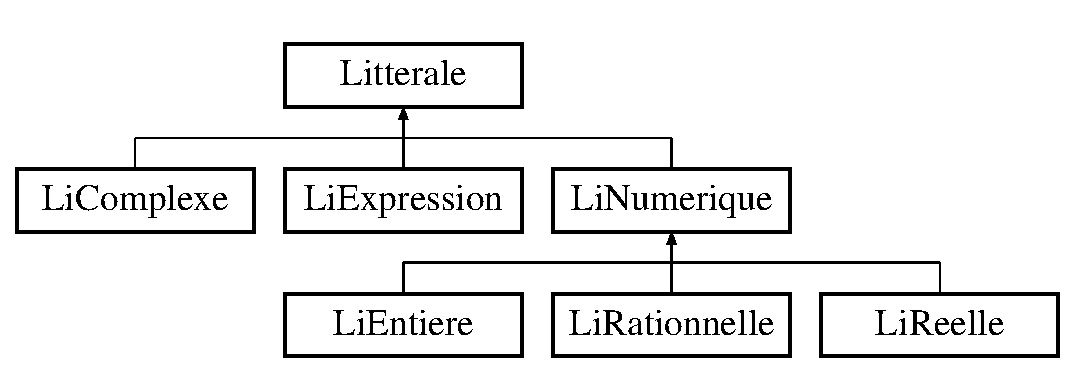
\includegraphics[height=3.000000cm]{class_litterale}
\end{center}
\end{figure}
\subsection*{Public Member Functions}
\begin{DoxyCompactItemize}
\item 
virtual \hyperlink{class_litterale_abd6b3faa8cda262bb5fab57e1e323090}{$\sim$\+Litterale} ()
\begin{DoxyCompactList}\small\item\em Destructor. \end{DoxyCompactList}\item 
virtual string \hyperlink{class_litterale_a3041839e5494df2c93bff2c5cb83ce1f}{to\+String} () const  =0
\begin{DoxyCompactList}\small\item\em \hyperlink{class_litterale_a3041839e5494df2c93bff2c5cb83ce1f}{to\+String()} method \end{DoxyCompactList}\item 
virtual bool \hyperlink{class_litterale_a535fc431d96954754b7a729404df4a79}{is\+Zero} () const  =0
\begin{DoxyCompactList}\small\item\em \hyperlink{class_litterale_a535fc431d96954754b7a729404df4a79}{is\+Zero()} method \end{DoxyCompactList}\item 
void \hyperlink{class_litterale_ae33587fb3c4a929c9ee29d9c6b49aea6}{afficher} (ostream \&f=cout) const 
\begin{DoxyCompactList}\small\item\em \hyperlink{class_litterale_ae33587fb3c4a929c9ee29d9c6b49aea6}{afficher()} method \end{DoxyCompactList}\item 
virtual int \hyperlink{class_litterale_a9cd3d639341cb797bcf2b6400d6ad43d}{get\+Value} () const 
\begin{DoxyCompactList}\small\item\em \hyperlink{class_litterale_a9cd3d639341cb797bcf2b6400d6ad43d}{get\+Value()} method \end{DoxyCompactList}\item 
virtual int \hyperlink{class_litterale_a6d3e582118775a3a0362154ae1a8cbda}{get\+Numerateur} () const 
\begin{DoxyCompactList}\small\item\em get\+Numerator() method \end{DoxyCompactList}\item 
virtual int \hyperlink{class_litterale_a68a07beac9e8a4e71d3920a4c6c27cc7}{get\+Denominateur} () const 
\begin{DoxyCompactList}\small\item\em get\+Denominator() method \end{DoxyCompactList}\item 
virtual double \hyperlink{class_litterale_aca56aad5f1a4a691337142e3f5a3b93d}{get\+Reel} () const 
\begin{DoxyCompactList}\small\item\em \hyperlink{class_litterale_aca56aad5f1a4a691337142e3f5a3b93d}{get\+Reel()} method \end{DoxyCompactList}\item 
virtual \hyperlink{class_litterale}{Litterale} $\ast$ \hyperlink{class_litterale_af4f96b09214b34ae26fe3f2722c42cc0}{operator+} (const \hyperlink{class_litterale}{Litterale} \&li) const  =0
\begin{DoxyCompactList}\small\item\em operator+ \end{DoxyCompactList}\item 
virtual \hyperlink{class_litterale}{Litterale} $\ast$ \hyperlink{class_litterale_a52eec71121af9c4bbf30011eccc87a68}{operator-\/} (const \hyperlink{class_litterale}{Litterale} \&li) const  =0
\begin{DoxyCompactList}\small\item\em operator-\/ \end{DoxyCompactList}\item 
virtual \hyperlink{class_litterale}{Litterale} $\ast$ \hyperlink{class_litterale_a91da4f609054b3146007291d199e1f33}{operator/} (const \hyperlink{class_litterale}{Litterale} \&li) const  =0
\begin{DoxyCompactList}\small\item\em operator/ \end{DoxyCompactList}\item 
virtual \hyperlink{class_litterale}{Litterale} $\ast$ \hyperlink{class_litterale_a54eb0d992188da6b490418bdd828b096}{operator$\ast$} (const \hyperlink{class_litterale}{Litterale} \&li) const  =0
\begin{DoxyCompactList}\small\item\em operator$\ast$ \end{DoxyCompactList}\item 
virtual \hyperlink{class_litterale}{Litterale} $\ast$ \hyperlink{class_litterale_a3d4832d994a32a36cb88f8a7d021b280}{operator==} (const \hyperlink{class_litterale}{Litterale} \&li) const  =0
\begin{DoxyCompactList}\small\item\em operator== \end{DoxyCompactList}\item 
virtual \hyperlink{class_litterale}{Litterale} $\ast$ \hyperlink{class_litterale_aec92913de9d127360897b0d644b5a44f}{operator!=} (const \hyperlink{class_litterale}{Litterale} \&li) const  =0
\begin{DoxyCompactList}\small\item\em operator!= \end{DoxyCompactList}\item 
virtual \hyperlink{class_litterale}{Litterale} $\ast$ \hyperlink{class_litterale_af70f373b306808959e234a366de8d799}{operator$<$=} (const \hyperlink{class_litterale}{Litterale} \&li) const  =0
\begin{DoxyCompactList}\small\item\em operator$<$= \end{DoxyCompactList}\item 
virtual \hyperlink{class_litterale}{Litterale} $\ast$ \hyperlink{class_litterale_af31c8ca0ecaccbc05718193d8858bc5d}{operator$>$=} (const \hyperlink{class_litterale}{Litterale} \&li) const  =0
\begin{DoxyCompactList}\small\item\em operator$>$= \end{DoxyCompactList}\item 
virtual \hyperlink{class_litterale}{Litterale} $\ast$ \hyperlink{class_litterale_a43ba11f1f3ee6cbf21cd2432708938f9}{operator$<$} (const \hyperlink{class_litterale}{Litterale} \&li) const  =0
\begin{DoxyCompactList}\small\item\em operator$<$ \end{DoxyCompactList}\item 
virtual \hyperlink{class_litterale}{Litterale} $\ast$ \hyperlink{class_litterale_a743719ab28de43c55449a90ccd55a95a}{operator$>$} (const \hyperlink{class_litterale}{Litterale} \&li) const  =0
\begin{DoxyCompactList}\small\item\em operator$>$ \end{DoxyCompactList}\item 
virtual \hyperlink{class_litterale}{Litterale} $\ast$ \hyperlink{class_litterale_ac9261e971a9d7d84137557d1cad94336}{Neg} ()=0
\begin{DoxyCompactList}\small\item\em N\+E\+G() method. \end{DoxyCompactList}\item 
virtual \hyperlink{class_litterale}{Litterale} $\ast$ \hyperlink{class_litterale_a4f02faabce1e1f46c4d34508de316a2b}{Num} ()=0
\begin{DoxyCompactList}\small\item\em N\+U\+M() method. \end{DoxyCompactList}\item 
virtual \hyperlink{class_litterale}{Litterale} $\ast$ \hyperlink{class_litterale_aedcaa806cc6b037371b25d12086503b8}{Den} ()=0
\begin{DoxyCompactList}\small\item\em D\+E\+N() method. \end{DoxyCompactList}\item 
virtual \hyperlink{class_litterale}{Litterale} $\ast$ \hyperlink{class_litterale_ac3ab556147c54f260be336fb53ecb52e}{Re} ()=0
\begin{DoxyCompactList}\small\item\em R\+E() method. \end{DoxyCompactList}\item 
virtual \hyperlink{class_litterale}{Litterale} $\ast$ \hyperlink{class_litterale_a8f0c2d98186c545f4f34ae07b9751f97}{Im} ()=0
\begin{DoxyCompactList}\small\item\em I\+M() method. \end{DoxyCompactList}\item 
virtual \hyperlink{class_litterale}{Litterale} $\ast$ \hyperlink{class_litterale_a2331619771c5cb74bee253e2c2cf62f5}{And} (const \hyperlink{class_litterale}{Litterale} $\ast$li)=0
\begin{DoxyCompactList}\small\item\em A\+N\+D() method. \end{DoxyCompactList}\item 
virtual \hyperlink{class_litterale}{Litterale} $\ast$ \hyperlink{class_litterale_a326ce76a35c3d29ad409c9491d5169a1}{Or} (const \hyperlink{class_litterale}{Litterale} $\ast$li)=0
\begin{DoxyCompactList}\small\item\em O\+R() method. \end{DoxyCompactList}\item 
virtual \hyperlink{class_litterale}{Litterale} $\ast$ \hyperlink{class_litterale_af44ae987ec5db62170efb3aec563c95c}{Not} ()=0
\begin{DoxyCompactList}\small\item\em N\+O\+T() method. \end{DoxyCompactList}\item 
virtual \hyperlink{class_litterale}{Litterale} $\ast$ {\bfseries Clone} () const  =0\hypertarget{class_litterale_a98f8da40c35c36275656d5bdb94482c5}{}\label{class_litterale_a98f8da40c35c36275656d5bdb94482c5}

\end{DoxyCompactItemize}


\subsection{Constructor \& Destructor Documentation}
\index{Litterale@{Litterale}!````~Litterale@{$\sim$\+Litterale}}
\index{````~Litterale@{$\sim$\+Litterale}!Litterale@{Litterale}}
\subsubsection[{\texorpdfstring{$\sim$\+Litterale()}{~Litterale()}}]{\setlength{\rightskip}{0pt plus 5cm}virtual Litterale\+::$\sim$\+Litterale (
\begin{DoxyParamCaption}
{}
\end{DoxyParamCaption}
)\hspace{0.3cm}{\ttfamily [inline]}, {\ttfamily [virtual]}}\hypertarget{class_litterale_abd6b3faa8cda262bb5fab57e1e323090}{}\label{class_litterale_abd6b3faa8cda262bb5fab57e1e323090}


Destructor. 

Virtual method (because of the \hyperlink{class_li_complexe}{Li\+Complexe} class) When a \hyperlink{class_litterale}{Litterale} object which points to a \hyperlink{class_li_complexe}{Li\+Complexe} object is deleted, the destructor of the \hyperlink{class_li_complexe}{Li\+Complexe} class needs to be called 

\subsection{Member Function Documentation}
\index{Litterale@{Litterale}!afficher@{afficher}}
\index{afficher@{afficher}!Litterale@{Litterale}}
\subsubsection[{\texorpdfstring{afficher(ostream \&f=cout) const }{afficher(ostream &f=cout) const }}]{\setlength{\rightskip}{0pt plus 5cm}void Litterale\+::afficher (
\begin{DoxyParamCaption}
\item[{ostream \&}]{f = {\ttfamily cout}}
\end{DoxyParamCaption}
) const\hspace{0.3cm}{\ttfamily [inline]}}\hypertarget{class_litterale_ae33587fb3c4a929c9ee29d9c6b49aea6}{}\label{class_litterale_ae33587fb3c4a929c9ee29d9c6b49aea6}


\hyperlink{class_litterale_ae33587fb3c4a929c9ee29d9c6b49aea6}{afficher()} method 

const method used to print the different \hyperlink{class_litterale}{Litterale} Call the \hyperlink{class_litterale_a3041839e5494df2c93bff2c5cb83ce1f}{to\+String()} method


\begin{DoxyParams}{Parameters}
{\em 1} & parameter of type ostream\& (default \+: cout) \\
\hline
\end{DoxyParams}
\begin{DoxyReturn}{Returns}
void 
\end{DoxyReturn}
\index{Litterale@{Litterale}!And@{And}}
\index{And@{And}!Litterale@{Litterale}}
\subsubsection[{\texorpdfstring{And(const Litterale $\ast$li)=0}{And(const Litterale *li)=0}}]{\setlength{\rightskip}{0pt plus 5cm}virtual {\bf Litterale}$\ast$ Litterale\+::\+And (
\begin{DoxyParamCaption}
\item[{const {\bf Litterale} $\ast$}]{li}
\end{DoxyParamCaption}
)\hspace{0.3cm}{\ttfamily [pure virtual]}}\hypertarget{class_litterale_a2331619771c5cb74bee253e2c2cf62f5}{}\label{class_litterale_a2331619771c5cb74bee253e2c2cf62f5}


A\+N\+D() method. 

Pure virtual method Const method (object should not be modified) Logic operator A\+ND


\begin{DoxyParams}{Parameters}
{\em const} & reference to \hyperlink{class_litterale}{Litterale} (parameter should not be modified) \\
\hline
\end{DoxyParams}
\begin{DoxyReturn}{Returns}
pointer to \hyperlink{class_litterale}{Litterale} 
\end{DoxyReturn}


Implemented in \hyperlink{class_li_entiere_acda292c445dfc7175a8c3112a2f626b6}{Li\+Entiere}, \hyperlink{class_li_expression_a6e29f5bd106989a72e8096d3481fd326}{Li\+Expression}, \hyperlink{class_li_rationnelle_adf47ed34fdf8cb4226064ac9599446ac}{Li\+Rationnelle}, \hyperlink{class_li_complexe_acf2840a901081b436f43045660d14362}{Li\+Complexe}, and \hyperlink{class_li_reelle_a02ffab7d9d66a3d19845155604d61611}{Li\+Reelle}.

\index{Litterale@{Litterale}!Den@{Den}}
\index{Den@{Den}!Litterale@{Litterale}}
\subsubsection[{\texorpdfstring{Den()=0}{Den()=0}}]{\setlength{\rightskip}{0pt plus 5cm}virtual {\bf Litterale}$\ast$ Litterale\+::\+Den (
\begin{DoxyParamCaption}
{}
\end{DoxyParamCaption}
)\hspace{0.3cm}{\ttfamily [pure virtual]}}\hypertarget{class_litterale_aedcaa806cc6b037371b25d12086503b8}{}\label{class_litterale_aedcaa806cc6b037371b25d12086503b8}


D\+E\+N() method. 

Pure virtual method Accessor to the denominator of Litterales


\begin{DoxyParams}{Parameters}
{\em no} & parameters \\
\hline
\end{DoxyParams}
\begin{DoxyReturn}{Returns}
pointer to \hyperlink{class_litterale}{Litterale} 
\end{DoxyReturn}


Implemented in \hyperlink{class_li_entiere_ac8936753e6ecfe460e14966b81f0b7e6}{Li\+Entiere}, \hyperlink{class_li_expression_ab135c92b3d0378fea00a60f096fab7d6}{Li\+Expression}, \hyperlink{class_li_rationnelle_afaa05daee860500829bb2f8bb0d3458f}{Li\+Rationnelle}, \hyperlink{class_li_complexe_aa4f828dac7bc5fbea088a289719943b6}{Li\+Complexe}, and \hyperlink{class_li_reelle_a546d4b22265cb69d2273bd62506ba55b}{Li\+Reelle}.

\index{Litterale@{Litterale}!get\+Denominateur@{get\+Denominateur}}
\index{get\+Denominateur@{get\+Denominateur}!Litterale@{Litterale}}
\subsubsection[{\texorpdfstring{get\+Denominateur() const }{getDenominateur() const }}]{\setlength{\rightskip}{0pt plus 5cm}virtual int Litterale\+::get\+Denominateur (
\begin{DoxyParamCaption}
{}
\end{DoxyParamCaption}
) const\hspace{0.3cm}{\ttfamily [inline]}, {\ttfamily [virtual]}}\hypertarget{class_litterale_a68a07beac9e8a4e71d3920a4c6c27cc7}{}\label{class_litterale_a68a07beac9e8a4e71d3920a4c6c27cc7}


get\+Denominator() method 

Virtual method Accessor for the \hyperlink{class_li_rationnelle}{Li\+Rationnelle} class (defined here to avoid dynamic\+\_\+casts)


\begin{DoxyParams}{Parameters}
{\em no} & parameters \\
\hline
\end{DoxyParams}
\begin{DoxyReturn}{Returns}
int 
\end{DoxyReturn}


Reimplemented in \hyperlink{class_li_rationnelle_aef5786f2be1ad1c301352d75c7eb14ed}{Li\+Rationnelle}, \hyperlink{class_li_entiere_aed4e11ecdfc99dfaba9f41e460ef71fb}{Li\+Entiere}, \hyperlink{class_li_expression_ab0c4fc0767e78b313d2ac4741bc9a8e7}{Li\+Expression}, and \hyperlink{class_li_reelle_a50d6d5764a8cff1ad1676db99c6f2115}{Li\+Reelle}.

\index{Litterale@{Litterale}!get\+Numerateur@{get\+Numerateur}}
\index{get\+Numerateur@{get\+Numerateur}!Litterale@{Litterale}}
\subsubsection[{\texorpdfstring{get\+Numerateur() const }{getNumerateur() const }}]{\setlength{\rightskip}{0pt plus 5cm}virtual int Litterale\+::get\+Numerateur (
\begin{DoxyParamCaption}
{}
\end{DoxyParamCaption}
) const\hspace{0.3cm}{\ttfamily [inline]}, {\ttfamily [virtual]}}\hypertarget{class_litterale_a6d3e582118775a3a0362154ae1a8cbda}{}\label{class_litterale_a6d3e582118775a3a0362154ae1a8cbda}


get\+Numerator() method 

Virtual method Accessor for the \hyperlink{class_li_rationnelle}{Li\+Rationnelle} class (defined here to avoid dynamic\+\_\+casts)


\begin{DoxyParams}{Parameters}
{\em no} & parameters \\
\hline
\end{DoxyParams}
\begin{DoxyReturn}{Returns}
int 
\end{DoxyReturn}


Reimplemented in \hyperlink{class_li_rationnelle_aeec109595a83168a8050b3f9608ac63e}{Li\+Rationnelle}, \hyperlink{class_li_entiere_af07e732cc94ac20f64d62031fe54cd06}{Li\+Entiere}, \hyperlink{class_li_expression_a5a4547ae8674412134264a8cd436e938}{Li\+Expression}, and \hyperlink{class_li_reelle_aced0465644e6ce7c67dca27ef32d1f80}{Li\+Reelle}.

\index{Litterale@{Litterale}!get\+Reel@{get\+Reel}}
\index{get\+Reel@{get\+Reel}!Litterale@{Litterale}}
\subsubsection[{\texorpdfstring{get\+Reel() const }{getReel() const }}]{\setlength{\rightskip}{0pt plus 5cm}virtual double Litterale\+::get\+Reel (
\begin{DoxyParamCaption}
{}
\end{DoxyParamCaption}
) const\hspace{0.3cm}{\ttfamily [inline]}, {\ttfamily [virtual]}}\hypertarget{class_litterale_aca56aad5f1a4a691337142e3f5a3b93d}{}\label{class_litterale_aca56aad5f1a4a691337142e3f5a3b93d}


\hyperlink{class_litterale_aca56aad5f1a4a691337142e3f5a3b93d}{get\+Reel()} method 

Virtual method Accessor for the \hyperlink{class_li_reelle}{Li\+Reelle} class (defined here to avoid dynamic\+\_\+casts)


\begin{DoxyParams}{Parameters}
{\em no} & parameters \\
\hline
\end{DoxyParams}
\begin{DoxyReturn}{Returns}
double 
\end{DoxyReturn}


Reimplemented in \hyperlink{class_li_rationnelle_a546fd77067d7ba3593b8bf9b05d7db5c}{Li\+Rationnelle}, \hyperlink{class_li_entiere_aa43ad42052b2adc31ff3b64cf541d8d7}{Li\+Entiere}, \hyperlink{class_li_expression_a6810603f331aa6a054df4e4d9f64ba4a}{Li\+Expression}, and \hyperlink{class_li_reelle_a2a172ac11b3d20715ba981163da203f3}{Li\+Reelle}.

\index{Litterale@{Litterale}!get\+Value@{get\+Value}}
\index{get\+Value@{get\+Value}!Litterale@{Litterale}}
\subsubsection[{\texorpdfstring{get\+Value() const }{getValue() const }}]{\setlength{\rightskip}{0pt plus 5cm}virtual int Litterale\+::get\+Value (
\begin{DoxyParamCaption}
{}
\end{DoxyParamCaption}
) const\hspace{0.3cm}{\ttfamily [inline]}, {\ttfamily [virtual]}}\hypertarget{class_litterale_a9cd3d639341cb797bcf2b6400d6ad43d}{}\label{class_litterale_a9cd3d639341cb797bcf2b6400d6ad43d}


\hyperlink{class_litterale_a9cd3d639341cb797bcf2b6400d6ad43d}{get\+Value()} method 

Virtual method Accessor for the \hyperlink{class_li_entiere}{Li\+Entiere} class (defined here to avoid dynamic\+\_\+casts)


\begin{DoxyParams}{Parameters}
{\em no} & parameters \\
\hline
\end{DoxyParams}
\begin{DoxyReturn}{Returns}
int 
\end{DoxyReturn}


Reimplemented in \hyperlink{class_li_rationnelle_aa84a9691ac8a8673b8397ce3fe1efcc0}{Li\+Rationnelle}, \hyperlink{class_li_expression_a17e0a77c27727e85d3784527c217827e}{Li\+Expression}, \hyperlink{class_li_entiere_a83bbae276cdb1946b18d913f99bab0e7}{Li\+Entiere}, and \hyperlink{class_li_reelle_a535bb0861646fbf417d05196e13092b0}{Li\+Reelle}.

\index{Litterale@{Litterale}!Im@{Im}}
\index{Im@{Im}!Litterale@{Litterale}}
\subsubsection[{\texorpdfstring{Im()=0}{Im()=0}}]{\setlength{\rightskip}{0pt plus 5cm}virtual {\bf Litterale}$\ast$ Litterale\+::\+Im (
\begin{DoxyParamCaption}
{}
\end{DoxyParamCaption}
)\hspace{0.3cm}{\ttfamily [pure virtual]}}\hypertarget{class_litterale_a8f0c2d98186c545f4f34ae07b9751f97}{}\label{class_litterale_a8f0c2d98186c545f4f34ae07b9751f97}


I\+M() method. 

Pure virtual method Accessor to the imaginary part of Litterales


\begin{DoxyParams}{Parameters}
{\em no} & parameters \\
\hline
\end{DoxyParams}
\begin{DoxyReturn}{Returns}
pointer to \hyperlink{class_litterale}{Litterale} 
\end{DoxyReturn}


Implemented in \hyperlink{class_li_entiere_a11df7bad558ba4a282c9b5331abad07f}{Li\+Entiere}, \hyperlink{class_li_rationnelle_aba3efd619ca23e4dfb3e9b79f34eb438}{Li\+Rationnelle}, \hyperlink{class_li_expression_ac9f9dae0e22ae52c5c8e92a3b4dc6a2a}{Li\+Expression}, \hyperlink{class_li_complexe_a57082c43306e5d43c69d037723d646e7}{Li\+Complexe}, and \hyperlink{class_li_reelle_a0e873df9175f1cd776529a0f2c00dcc4}{Li\+Reelle}.

\index{Litterale@{Litterale}!is\+Zero@{is\+Zero}}
\index{is\+Zero@{is\+Zero}!Litterale@{Litterale}}
\subsubsection[{\texorpdfstring{is\+Zero() const  =0}{isZero() const  =0}}]{\setlength{\rightskip}{0pt plus 5cm}virtual bool Litterale\+::is\+Zero (
\begin{DoxyParamCaption}
{}
\end{DoxyParamCaption}
) const\hspace{0.3cm}{\ttfamily [pure virtual]}}\hypertarget{class_litterale_a535fc431d96954754b7a729404df4a79}{}\label{class_litterale_a535fc431d96954754b7a729404df4a79}


\hyperlink{class_litterale_a535fc431d96954754b7a729404df4a79}{is\+Zero()} method 

Pure virtual method Used to inform us if a the attributs of a class are 0 This method have to be defined in the inherited classes


\begin{DoxyParams}{Parameters}
{\em no} & parameter \\
\hline
\end{DoxyParams}
\begin{DoxyReturn}{Returns}
bool 
\end{DoxyReturn}


Implemented in \hyperlink{class_li_rationnelle_a3c9713b43958f09c4e2a7506fd9fdee8}{Li\+Rationnelle}, \hyperlink{class_li_complexe_a6bcabbf5bcf296fdb048c9be278f175a}{Li\+Complexe}, \hyperlink{class_li_entiere_a21645454b355997a8a73156900546cbd}{Li\+Entiere}, \hyperlink{class_li_reelle_a0470145a910d993012e9f6c5f8896b08}{Li\+Reelle}, and \hyperlink{class_li_expression_ac6e982f0986c28b01a1221830bce20eb}{Li\+Expression}.

\index{Litterale@{Litterale}!Neg@{Neg}}
\index{Neg@{Neg}!Litterale@{Litterale}}
\subsubsection[{\texorpdfstring{Neg()=0}{Neg()=0}}]{\setlength{\rightskip}{0pt plus 5cm}virtual {\bf Litterale}$\ast$ Litterale\+::\+Neg (
\begin{DoxyParamCaption}
{}
\end{DoxyParamCaption}
)\hspace{0.3cm}{\ttfamily [pure virtual]}}\hypertarget{class_litterale_ac9261e971a9d7d84137557d1cad94336}{}\label{class_litterale_ac9261e971a9d7d84137557d1cad94336}


N\+E\+G() method. 

Pure virtual method Changes the sign of the attributes of a \hyperlink{class_litterale}{Litterale}


\begin{DoxyParams}{Parameters}
{\em no} & parameters \\
\hline
\end{DoxyParams}
\begin{DoxyReturn}{Returns}
pointer to \hyperlink{class_litterale}{Litterale} 
\end{DoxyReturn}


Implemented in \hyperlink{class_li_expression_a0bf45253ed1ac7d76d0950f5368f634c}{Li\+Expression}, \hyperlink{class_li_entiere_a708a535d92593c881c749f70bbdfacde}{Li\+Entiere}, \hyperlink{class_li_rationnelle_a102af5b1669d85ba3bc0f93286e5f75f}{Li\+Rationnelle}, \hyperlink{class_li_complexe_a71954f11bfc89933860279cb932f68a9}{Li\+Complexe}, and \hyperlink{class_li_reelle_a68bbd97118395e887735caf4d8248d0e}{Li\+Reelle}.

\index{Litterale@{Litterale}!Not@{Not}}
\index{Not@{Not}!Litterale@{Litterale}}
\subsubsection[{\texorpdfstring{Not()=0}{Not()=0}}]{\setlength{\rightskip}{0pt plus 5cm}virtual {\bf Litterale}$\ast$ Litterale\+::\+Not (
\begin{DoxyParamCaption}
{}
\end{DoxyParamCaption}
)\hspace{0.3cm}{\ttfamily [pure virtual]}}\hypertarget{class_litterale_af44ae987ec5db62170efb3aec563c95c}{}\label{class_litterale_af44ae987ec5db62170efb3aec563c95c}


N\+O\+T() method. 

Pure virtual method Const method (object should not be modified) Logic operator N\+OT


\begin{DoxyParams}{Parameters}
{\em no} & parameter \\
\hline
\end{DoxyParams}
\begin{DoxyReturn}{Returns}
pointer to \hyperlink{class_litterale}{Litterale} 
\end{DoxyReturn}


Implemented in \hyperlink{class_li_entiere_a9e7e16765f03404215bff26dcc9b44c2}{Li\+Entiere}, \hyperlink{class_li_expression_ac07a8597d82ce267204cb3bbd3c6fba1}{Li\+Expression}, \hyperlink{class_li_rationnelle_ace9603d446eac2df241eadcf55ad764e}{Li\+Rationnelle}, \hyperlink{class_li_complexe_a37011cb1b7e5d4e9a2e22f217eb463f2}{Li\+Complexe}, and \hyperlink{class_li_reelle_a85e6a8f3389148978a21dc70774d66e4}{Li\+Reelle}.

\index{Litterale@{Litterale}!Num@{Num}}
\index{Num@{Num}!Litterale@{Litterale}}
\subsubsection[{\texorpdfstring{Num()=0}{Num()=0}}]{\setlength{\rightskip}{0pt plus 5cm}virtual {\bf Litterale}$\ast$ Litterale\+::\+Num (
\begin{DoxyParamCaption}
{}
\end{DoxyParamCaption}
)\hspace{0.3cm}{\ttfamily [pure virtual]}}\hypertarget{class_litterale_a4f02faabce1e1f46c4d34508de316a2b}{}\label{class_litterale_a4f02faabce1e1f46c4d34508de316a2b}


N\+U\+M() method. 

Pure virtual method Accessor to the numerator of Litterales


\begin{DoxyParams}{Parameters}
{\em no} & parameters \\
\hline
\end{DoxyParams}
\begin{DoxyReturn}{Returns}
pointer to \hyperlink{class_litterale}{Litterale} 
\end{DoxyReturn}


Implemented in \hyperlink{class_li_entiere_a482e5cb35a25e22bd243490e7444bf96}{Li\+Entiere}, \hyperlink{class_li_expression_aff040ab50e34119fc3ef87a3810857dd}{Li\+Expression}, \hyperlink{class_li_rationnelle_a1a7a534097e249eccff3fd8a0f37c722}{Li\+Rationnelle}, \hyperlink{class_li_complexe_a7068b0171c0e0efb6ba803247f1aceca}{Li\+Complexe}, and \hyperlink{class_li_reelle_aa4184e221af015edfb3e53cede494746}{Li\+Reelle}.

\index{Litterale@{Litterale}!operator"!=@{operator"!=}}
\index{operator"!=@{operator"!=}!Litterale@{Litterale}}
\subsubsection[{\texorpdfstring{operator"!=(const Litterale \&li) const  =0}{operator!=(const Litterale &li) const  =0}}]{\setlength{\rightskip}{0pt plus 5cm}virtual {\bf Litterale}$\ast$ Litterale\+::operator!= (
\begin{DoxyParamCaption}
\item[{const {\bf Litterale} \&}]{li}
\end{DoxyParamCaption}
) const\hspace{0.3cm}{\ttfamily [pure virtual]}}\hypertarget{class_litterale_aec92913de9d127360897b0d644b5a44f}{}\label{class_litterale_aec92913de9d127360897b0d644b5a44f}


operator!= 

Pure virtual method Const method (object should not be modified) overload of the operator != Used to test if 2 litterales are not equal


\begin{DoxyParams}{Parameters}
{\em const} & reference to \hyperlink{class_litterale}{Litterale} (parameter should not be modified) \\
\hline
\end{DoxyParams}
\begin{DoxyReturn}{Returns}
pointer to \hyperlink{class_litterale}{Litterale} 
\end{DoxyReturn}


Implemented in \hyperlink{class_li_entiere_af14a5d2ad57e93da2176d4316e5e2330}{Li\+Entiere}, \hyperlink{class_li_expression_a109d27f2e3a8717a0cd391db8042f3d7}{Li\+Expression}, \hyperlink{class_li_rationnelle_a6c9e22c2e191a15a334377b1feb0c8ef}{Li\+Rationnelle}, \hyperlink{class_li_reelle_a1374d797764cae650c9fc7b164811278}{Li\+Reelle}, and \hyperlink{class_li_complexe_a85020ff32c533327425c70ebbf804abf}{Li\+Complexe}.

\index{Litterale@{Litterale}!operator$\ast$@{operator$\ast$}}
\index{operator$\ast$@{operator$\ast$}!Litterale@{Litterale}}
\subsubsection[{\texorpdfstring{operator$\ast$(const Litterale \&li) const  =0}{operator*(const Litterale &li) const  =0}}]{\setlength{\rightskip}{0pt plus 5cm}virtual {\bf Litterale}$\ast$ Litterale\+::operator$\ast$ (
\begin{DoxyParamCaption}
\item[{const {\bf Litterale} \&}]{li}
\end{DoxyParamCaption}
) const\hspace{0.3cm}{\ttfamily [pure virtual]}}\hypertarget{class_litterale_a54eb0d992188da6b490418bdd828b096}{}\label{class_litterale_a54eb0d992188da6b490418bdd828b096}


operator$\ast$ 

Pure virtual method Const method (object should not be modified) overload of the operator $\ast$ Used to multiply 2 litterales


\begin{DoxyParams}{Parameters}
{\em const} & reference to \hyperlink{class_litterale}{Litterale} (parameter should not be modified) \\
\hline
\end{DoxyParams}
\begin{DoxyReturn}{Returns}
pointer to \hyperlink{class_litterale}{Litterale} 
\end{DoxyReturn}


Implemented in \hyperlink{class_li_entiere_a976f7f29b27e02770a8efc6278da4255}{Li\+Entiere}, \hyperlink{class_li_rationnelle_a32577e06c8316232a45147b36d9cde06}{Li\+Rationnelle}, \hyperlink{class_li_expression_a14d8c244f1d0a5035781e999220f6972}{Li\+Expression}, \hyperlink{class_li_reelle_a3a9597d7bb98c85ff27a68498cc54533}{Li\+Reelle}, and \hyperlink{class_li_complexe_a88ad289cf55d8e6d89f0d77cf09d2ccf}{Li\+Complexe}.

\index{Litterale@{Litterale}!operator+@{operator+}}
\index{operator+@{operator+}!Litterale@{Litterale}}
\subsubsection[{\texorpdfstring{operator+(const Litterale \&li) const  =0}{operator+(const Litterale &li) const  =0}}]{\setlength{\rightskip}{0pt plus 5cm}virtual {\bf Litterale}$\ast$ Litterale\+::operator+ (
\begin{DoxyParamCaption}
\item[{const {\bf Litterale} \&}]{li}
\end{DoxyParamCaption}
) const\hspace{0.3cm}{\ttfamily [pure virtual]}}\hypertarget{class_litterale_af4f96b09214b34ae26fe3f2722c42cc0}{}\label{class_litterale_af4f96b09214b34ae26fe3f2722c42cc0}


operator+ 

Pure virtual method Const method (object sould not be modified) overload of the operator + Used to add 2 litterales


\begin{DoxyParams}{Parameters}
{\em const} & reference to \hyperlink{class_litterale}{Litterale} (parameter sould not be modified) \\
\hline
\end{DoxyParams}
\begin{DoxyReturn}{Returns}
pointer to \hyperlink{class_litterale}{Litterale} 
\end{DoxyReturn}


Implemented in \hyperlink{class_li_rationnelle_a6c33888d3b84585c4ca636f592d05b2f}{Li\+Rationnelle}, \hyperlink{class_li_entiere_a9dd8dc1327e46ea3486d02520c5d85c8}{Li\+Entiere}, \hyperlink{class_li_expression_aba0fbbab32512bad7e67aa23d2e50318}{Li\+Expression}, \hyperlink{class_li_reelle_afb5b649702e7b1a87937d38d0034546f}{Li\+Reelle}, and \hyperlink{class_li_complexe_a10fc45528f4f674e5afdddcd49cfefe8}{Li\+Complexe}.

\index{Litterale@{Litterale}!operator-\/@{operator-\/}}
\index{operator-\/@{operator-\/}!Litterale@{Litterale}}
\subsubsection[{\texorpdfstring{operator-\/(const Litterale \&li) const  =0}{operator-(const Litterale &li) const  =0}}]{\setlength{\rightskip}{0pt plus 5cm}virtual {\bf Litterale}$\ast$ Litterale\+::operator-\/ (
\begin{DoxyParamCaption}
\item[{const {\bf Litterale} \&}]{li}
\end{DoxyParamCaption}
) const\hspace{0.3cm}{\ttfamily [pure virtual]}}\hypertarget{class_litterale_a52eec71121af9c4bbf30011eccc87a68}{}\label{class_litterale_a52eec71121af9c4bbf30011eccc87a68}


operator-\/ 

Pure virtual method Const method (object should not be modified) overload of the operator -\/ Used to substract 2 litterales


\begin{DoxyParams}{Parameters}
{\em const} & reference to \hyperlink{class_litterale}{Litterale} (parameter should not be modified) \\
\hline
\end{DoxyParams}
\begin{DoxyReturn}{Returns}
pointer to \hyperlink{class_litterale}{Litterale} 
\end{DoxyReturn}


Implemented in \hyperlink{class_li_rationnelle_a8988443214ef0712ea1f48599cfd1168}{Li\+Rationnelle}, \hyperlink{class_li_entiere_a5b1f7fd5e9064c96c1b260a740f6b425}{Li\+Entiere}, \hyperlink{class_li_expression_a459ed09d7f610ff88e606fc95e0b22a5}{Li\+Expression}, \hyperlink{class_li_reelle_a8347d9889eaaf4b156ca1f4684a14679}{Li\+Reelle}, and \hyperlink{class_li_complexe_aafe560e78d42938bce8e42672850f187}{Li\+Complexe}.

\index{Litterale@{Litterale}!operator/@{operator/}}
\index{operator/@{operator/}!Litterale@{Litterale}}
\subsubsection[{\texorpdfstring{operator/(const Litterale \&li) const  =0}{operator/(const Litterale &li) const  =0}}]{\setlength{\rightskip}{0pt plus 5cm}virtual {\bf Litterale}$\ast$ Litterale\+::operator/ (
\begin{DoxyParamCaption}
\item[{const {\bf Litterale} \&}]{li}
\end{DoxyParamCaption}
) const\hspace{0.3cm}{\ttfamily [pure virtual]}}\hypertarget{class_litterale_a91da4f609054b3146007291d199e1f33}{}\label{class_litterale_a91da4f609054b3146007291d199e1f33}


operator/ 

Pure virtual method Const method (object should not be modified) overload of the operator / Used to divid 2 litterales


\begin{DoxyParams}{Parameters}
{\em const} & reference to \hyperlink{class_litterale}{Litterale} (parameter should not be modified) \\
\hline
\end{DoxyParams}
\begin{DoxyReturn}{Returns}
pointer to \hyperlink{class_litterale}{Litterale} 
\end{DoxyReturn}


Implemented in \hyperlink{class_li_rationnelle_a0c072bf37fa144a665fc30b36eba0a4c}{Li\+Rationnelle}, \hyperlink{class_li_entiere_a27d5f34f659e44b29d30f28aeda4db42}{Li\+Entiere}, \hyperlink{class_li_expression_a6d6c07034ea7c50301164e27d1af48fc}{Li\+Expression}, \hyperlink{class_li_reelle_affc5e3fd0084475152cba8cc477dc1af}{Li\+Reelle}, and \hyperlink{class_li_complexe_ab9dbace3f0fbd634a6258c4bcb5dc659}{Li\+Complexe}.

\index{Litterale@{Litterale}!operator$<$@{operator$<$}}
\index{operator$<$@{operator$<$}!Litterale@{Litterale}}
\subsubsection[{\texorpdfstring{operator$<$(const Litterale \&li) const  =0}{operator<(const Litterale &li) const  =0}}]{\setlength{\rightskip}{0pt plus 5cm}virtual {\bf Litterale}$\ast$ Litterale\+::operator$<$ (
\begin{DoxyParamCaption}
\item[{const {\bf Litterale} \&}]{li}
\end{DoxyParamCaption}
) const\hspace{0.3cm}{\ttfamily [pure virtual]}}\hypertarget{class_litterale_a43ba11f1f3ee6cbf21cd2432708938f9}{}\label{class_litterale_a43ba11f1f3ee6cbf21cd2432708938f9}


operator$<$ 

Pure virtual method Const method (object should not be modified) overload of the operator $<$ Used to compare 2 litterales


\begin{DoxyParams}{Parameters}
{\em const} & reference to \hyperlink{class_litterale}{Litterale} (parameter should not be modified) \\
\hline
\end{DoxyParams}
\begin{DoxyReturn}{Returns}
pointer to \hyperlink{class_litterale}{Litterale} 
\end{DoxyReturn}


Implemented in \hyperlink{class_li_entiere_a6446d0a2f619c160cf6a802c531d7d26}{Li\+Entiere}, \hyperlink{class_li_expression_aa0182e19cd3c065f7da2318fdbd261fe}{Li\+Expression}, \hyperlink{class_li_rationnelle_a7750712cfefeb74693b9d7e0c9db40e6}{Li\+Rationnelle}, \hyperlink{class_li_reelle_a0132f313a6dd67a1f82f8e6373062b41}{Li\+Reelle}, and \hyperlink{class_li_complexe_acb3d4e0f6636270f861490c465d07711}{Li\+Complexe}.

\index{Litterale@{Litterale}!operator$<$=@{operator$<$=}}
\index{operator$<$=@{operator$<$=}!Litterale@{Litterale}}
\subsubsection[{\texorpdfstring{operator$<$=(const Litterale \&li) const  =0}{operator<=(const Litterale &li) const  =0}}]{\setlength{\rightskip}{0pt plus 5cm}virtual {\bf Litterale}$\ast$ Litterale\+::operator$<$= (
\begin{DoxyParamCaption}
\item[{const {\bf Litterale} \&}]{li}
\end{DoxyParamCaption}
) const\hspace{0.3cm}{\ttfamily [pure virtual]}}\hypertarget{class_litterale_af70f373b306808959e234a366de8d799}{}\label{class_litterale_af70f373b306808959e234a366de8d799}


operator$<$= 

Pure virtual method Const method (object should not be modified) overload of the operator $<$= Used to compare 2 litterales


\begin{DoxyParams}{Parameters}
{\em const} & reference to \hyperlink{class_litterale}{Litterale} (parameter should not be modified) \\
\hline
\end{DoxyParams}
\begin{DoxyReturn}{Returns}
pointer to \hyperlink{class_litterale}{Litterale} 
\end{DoxyReturn}


Implemented in \hyperlink{class_li_entiere_a90a3b7b2f1ef1ea18faa50cd7150f141}{Li\+Entiere}, \hyperlink{class_li_expression_a2803c38127ed58e1d8148e06e079dbb4}{Li\+Expression}, \hyperlink{class_li_rationnelle_a74044fa6f0d605d5bd9c806b14f34391}{Li\+Rationnelle}, \hyperlink{class_li_reelle_a49bdd04d02271740a65eca555df3fbcd}{Li\+Reelle}, and \hyperlink{class_li_complexe_ae749d5d340b4bf8e878442a38caa78c1}{Li\+Complexe}.

\index{Litterale@{Litterale}!operator==@{operator==}}
\index{operator==@{operator==}!Litterale@{Litterale}}
\subsubsection[{\texorpdfstring{operator==(const Litterale \&li) const  =0}{operator==(const Litterale &li) const  =0}}]{\setlength{\rightskip}{0pt plus 5cm}virtual {\bf Litterale}$\ast$ Litterale\+::operator== (
\begin{DoxyParamCaption}
\item[{const {\bf Litterale} \&}]{li}
\end{DoxyParamCaption}
) const\hspace{0.3cm}{\ttfamily [pure virtual]}}\hypertarget{class_litterale_a3d4832d994a32a36cb88f8a7d021b280}{}\label{class_litterale_a3d4832d994a32a36cb88f8a7d021b280}


operator== 

Pure virtual method Const method (object should not be modified) overload of the operator == Used to test if 2 litterales are equal


\begin{DoxyParams}{Parameters}
{\em const} & reference to \hyperlink{class_litterale}{Litterale} (parameter should not be modified) \\
\hline
\end{DoxyParams}
\begin{DoxyReturn}{Returns}
pointer to \hyperlink{class_litterale}{Litterale} 
\end{DoxyReturn}


Implemented in \hyperlink{class_li_entiere_a27b8284b91bca5d9113676b7e9fd04d2}{Li\+Entiere}, \hyperlink{class_li_expression_a30334b98ebe99c3b06596b964b74aa2b}{Li\+Expression}, \hyperlink{class_li_rationnelle_a27349b75404a5b881da73f5a7362a6a8}{Li\+Rationnelle}, \hyperlink{class_li_reelle_a1e70861ad1af93c6639a3f6bd153f3ee}{Li\+Reelle}, and \hyperlink{class_li_complexe_a80fb4bf75402d5d1b8f1a3b9622b9047}{Li\+Complexe}.

\index{Litterale@{Litterale}!operator$>$@{operator$>$}}
\index{operator$>$@{operator$>$}!Litterale@{Litterale}}
\subsubsection[{\texorpdfstring{operator$>$(const Litterale \&li) const  =0}{operator>(const Litterale &li) const  =0}}]{\setlength{\rightskip}{0pt plus 5cm}virtual {\bf Litterale}$\ast$ Litterale\+::operator$>$ (
\begin{DoxyParamCaption}
\item[{const {\bf Litterale} \&}]{li}
\end{DoxyParamCaption}
) const\hspace{0.3cm}{\ttfamily [pure virtual]}}\hypertarget{class_litterale_a743719ab28de43c55449a90ccd55a95a}{}\label{class_litterale_a743719ab28de43c55449a90ccd55a95a}


operator$>$ 

Pure virtual method Const method (object should not be modified) overload of the operator $>$ Used to compare 2 litterales


\begin{DoxyParams}{Parameters}
{\em const} & reference to \hyperlink{class_litterale}{Litterale} (parameter should not be modified) \\
\hline
\end{DoxyParams}
\begin{DoxyReturn}{Returns}
pointer to \hyperlink{class_litterale}{Litterale} 
\end{DoxyReturn}


Implemented in \hyperlink{class_li_entiere_a92f1f5e097a794670463127a638a2f7b}{Li\+Entiere}, \hyperlink{class_li_expression_a31d73a19962932144004d181dd46a203}{Li\+Expression}, \hyperlink{class_li_rationnelle_ae3be0f9aa5b254c43b198b658366d526}{Li\+Rationnelle}, \hyperlink{class_li_complexe_a8b7b532a469c8e2abe976070d7433666}{Li\+Complexe}, and \hyperlink{class_li_reelle_acc5a25403b3929dbb690ef2a583d68c2}{Li\+Reelle}.

\index{Litterale@{Litterale}!operator$>$=@{operator$>$=}}
\index{operator$>$=@{operator$>$=}!Litterale@{Litterale}}
\subsubsection[{\texorpdfstring{operator$>$=(const Litterale \&li) const  =0}{operator>=(const Litterale &li) const  =0}}]{\setlength{\rightskip}{0pt plus 5cm}virtual {\bf Litterale}$\ast$ Litterale\+::operator$>$= (
\begin{DoxyParamCaption}
\item[{const {\bf Litterale} \&}]{li}
\end{DoxyParamCaption}
) const\hspace{0.3cm}{\ttfamily [pure virtual]}}\hypertarget{class_litterale_af31c8ca0ecaccbc05718193d8858bc5d}{}\label{class_litterale_af31c8ca0ecaccbc05718193d8858bc5d}


operator$>$= 

Pure virtual method Const method (object should not be modified) overload of the operator $>$= Used to compare 2 litterales


\begin{DoxyParams}{Parameters}
{\em const} & reference to \hyperlink{class_litterale}{Litterale} (parameter should not be modified) \\
\hline
\end{DoxyParams}
\begin{DoxyReturn}{Returns}
pointer to \hyperlink{class_litterale}{Litterale} 
\end{DoxyReturn}


Implemented in \hyperlink{class_li_entiere_af4494bc2dda7b1ff2301b43f19dbc197}{Li\+Entiere}, \hyperlink{class_li_expression_a9559555748722ee6f1a384527fef29a1}{Li\+Expression}, \hyperlink{class_li_rationnelle_a40b97ae950c490bde9f0325dbdfb268d}{Li\+Rationnelle}, \hyperlink{class_li_reelle_a2b2e23fae32215d966041d06e17edfa2}{Li\+Reelle}, and \hyperlink{class_li_complexe_a5c67194eb76e8760ce6dfec0e89f477a}{Li\+Complexe}.

\index{Litterale@{Litterale}!Or@{Or}}
\index{Or@{Or}!Litterale@{Litterale}}
\subsubsection[{\texorpdfstring{Or(const Litterale $\ast$li)=0}{Or(const Litterale *li)=0}}]{\setlength{\rightskip}{0pt plus 5cm}virtual {\bf Litterale}$\ast$ Litterale\+::\+Or (
\begin{DoxyParamCaption}
\item[{const {\bf Litterale} $\ast$}]{li}
\end{DoxyParamCaption}
)\hspace{0.3cm}{\ttfamily [pure virtual]}}\hypertarget{class_litterale_a326ce76a35c3d29ad409c9491d5169a1}{}\label{class_litterale_a326ce76a35c3d29ad409c9491d5169a1}


O\+R() method. 

Pure virtual method Const method (object should not be modified) Logic operator OR


\begin{DoxyParams}{Parameters}
{\em const} & reference to \hyperlink{class_litterale}{Litterale} (parameter should not be modified) \\
\hline
\end{DoxyParams}
\begin{DoxyReturn}{Returns}
pointer to \hyperlink{class_litterale}{Litterale} 
\end{DoxyReturn}


Implemented in \hyperlink{class_li_entiere_a74d7045bfc273fa6dab333b4bd832b19}{Li\+Entiere}, \hyperlink{class_li_expression_a12cb399c149c2b5383ec7207bd04ed8a}{Li\+Expression}, \hyperlink{class_li_rationnelle_a102aafbfd4b9ab4c1d1a4b666b9ae678}{Li\+Rationnelle}, \hyperlink{class_li_complexe_a4e05098ec1cdc4b6fd8bba10875181dd}{Li\+Complexe}, and \hyperlink{class_li_reelle_a0b55f57589414fdcea4120d9971cb837}{Li\+Reelle}.

\index{Litterale@{Litterale}!Re@{Re}}
\index{Re@{Re}!Litterale@{Litterale}}
\subsubsection[{\texorpdfstring{Re()=0}{Re()=0}}]{\setlength{\rightskip}{0pt plus 5cm}virtual {\bf Litterale}$\ast$ Litterale\+::\+Re (
\begin{DoxyParamCaption}
{}
\end{DoxyParamCaption}
)\hspace{0.3cm}{\ttfamily [pure virtual]}}\hypertarget{class_litterale_ac3ab556147c54f260be336fb53ecb52e}{}\label{class_litterale_ac3ab556147c54f260be336fb53ecb52e}


R\+E() method. 

Pure virtual method Accessor to the real part of Litterales


\begin{DoxyParams}{Parameters}
{\em no} & parameters \\
\hline
\end{DoxyParams}
\begin{DoxyReturn}{Returns}
pointer to \hyperlink{class_litterale}{Litterale} 
\end{DoxyReturn}


Implemented in \hyperlink{class_li_entiere_a6751154aae61b70ef2330a1e9155ed1a}{Li\+Entiere}, \hyperlink{class_li_expression_ae1a4046463009818bd96794ba65bd6b4}{Li\+Expression}, \hyperlink{class_li_rationnelle_aa1eb24b28a4df2145a315bdd71455754}{Li\+Rationnelle}, \hyperlink{class_li_complexe_ad93d70af2512c0e835c29677c12c419a}{Li\+Complexe}, and \hyperlink{class_li_reelle_ad7c72bce1be331de508c60eee2800b4a}{Li\+Reelle}.

\index{Litterale@{Litterale}!to\+String@{to\+String}}
\index{to\+String@{to\+String}!Litterale@{Litterale}}
\subsubsection[{\texorpdfstring{to\+String() const  =0}{toString() const  =0}}]{\setlength{\rightskip}{0pt plus 5cm}virtual string Litterale\+::to\+String (
\begin{DoxyParamCaption}
{}
\end{DoxyParamCaption}
) const\hspace{0.3cm}{\ttfamily [pure virtual]}}\hypertarget{class_litterale_a3041839e5494df2c93bff2c5cb83ce1f}{}\label{class_litterale_a3041839e5494df2c93bff2c5cb83ce1f}


\hyperlink{class_litterale_a3041839e5494df2c93bff2c5cb83ce1f}{to\+String()} method 

Pure virtual method used in the \hyperlink{class_litterale_ae33587fb3c4a929c9ee29d9c6b49aea6}{afficher()} method This method have to be defined in the inherited classes


\begin{DoxyParams}{Parameters}
{\em no} & parameter \\
\hline
\end{DoxyParams}
\begin{DoxyReturn}{Returns}
string 
\end{DoxyReturn}


Implemented in \hyperlink{class_li_rationnelle_a2ef7aa4c19e3433794c251cc61296f58}{Li\+Rationnelle}, \hyperlink{class_li_complexe_a5490d27f24fd273c8a3f5cc28e22d6d8}{Li\+Complexe}, \hyperlink{class_li_entiere_a48fceee2e4f1d481b923ebb28a085baf}{Li\+Entiere}, \hyperlink{class_li_reelle_ad78df00afab6b86f6b0ec966f848c872}{Li\+Reelle}, \hyperlink{class_li_expression_afbf36946d48981027d8af7685c950a9b}{Li\+Expression}, and \hyperlink{class_li_numerique_ad40fe29de93bcf18cc2cd088abcb728b}{Li\+Numerique}.



The documentation for this class was generated from the following file\+:\begin{DoxyCompactItemize}
\item 
\hyperlink{litterale_8h}{litterale.\+h}\end{DoxyCompactItemize}

\hypertarget{class_main_window}{}\section{Main\+Window Class Reference}
\label{class_main_window}\index{Main\+Window@{Main\+Window}}
Inheritance diagram for Main\+Window\+:\begin{figure}[H]
\begin{center}
\leavevmode
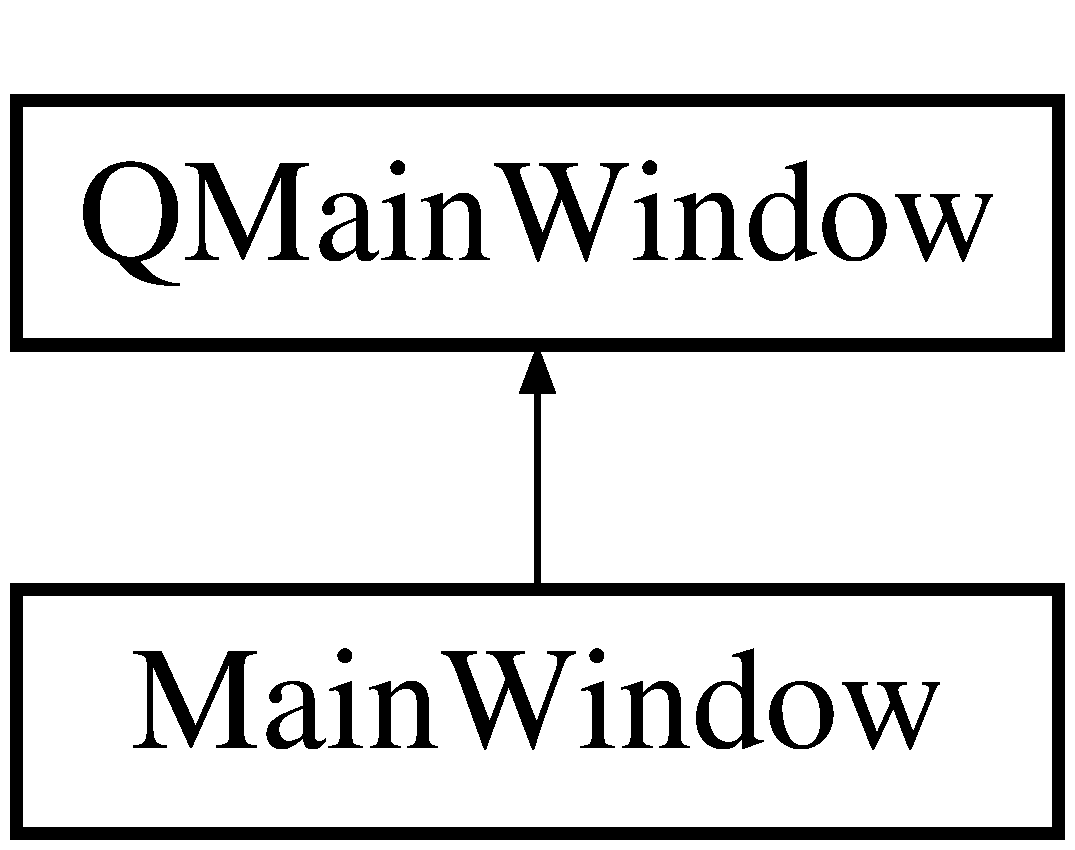
\includegraphics[height=2.000000cm]{class_main_window}
\end{center}
\end{figure}
\subsection*{Public Slots}
\begin{DoxyCompactItemize}
\item 
void {\bfseries refresh} ()\hypertarget{class_main_window_ab27297114529e4c16d6d8d7a54927a0e}{}\label{class_main_window_ab27297114529e4c16d6d8d7a54927a0e}

\item 
void {\bfseries get\+Next\+Commande} ()\hypertarget{class_main_window_ae9ba81c937937c6218a77ba0ac7a9461}{}\label{class_main_window_ae9ba81c937937c6218a77ba0ac7a9461}

\item 
void {\bfseries playsound} ()\hypertarget{class_main_window_a7d08f1de7502c6b1ff684f85e6009a37}{}\label{class_main_window_a7d08f1de7502c6b1ff684f85e6009a37}

\end{DoxyCompactItemize}
\subsection*{Public Member Functions}
\begin{DoxyCompactItemize}
\item 
\hyperlink{class_main_window_a8b244be8b7b7db1b08de2a2acb9409db}{Main\+Window} (Q\+Widget $\ast$parent=0)
\end{DoxyCompactItemize}


\subsection{Constructor \& Destructor Documentation}
\index{Main\+Window@{Main\+Window}!Main\+Window@{Main\+Window}}
\index{Main\+Window@{Main\+Window}!Main\+Window@{Main\+Window}}
\subsubsection[{\texorpdfstring{Main\+Window(\+Q\+Widget $\ast$parent=0)}{MainWindow(QWidget *parent=0)}}]{\setlength{\rightskip}{0pt plus 5cm}Main\+Window\+::\+Main\+Window (
\begin{DoxyParamCaption}
\item[{Q\+Widget $\ast$}]{parent = {\ttfamily 0}}
\end{DoxyParamCaption}
)\hspace{0.3cm}{\ttfamily [explicit]}}\hypertarget{class_main_window_a8b244be8b7b7db1b08de2a2acb9409db}{}\label{class_main_window_a8b244be8b7b7db1b08de2a2acb9409db}
I\+N\+I\+T\+I\+A\+L\+I\+Z\+A\+T\+I\+ON OF T\+HE A\+T\+T\+R\+I\+B\+U\+T\+ES

G\+R\+A\+P\+H\+IC I\+N\+I\+T\+I\+A\+L\+I\+Z\+A\+T\+I\+O\+Ns 

The documentation for this class was generated from the following files\+:\begin{DoxyCompactItemize}
\item 
mainwindow.\+h\item 
mainwindow.\+cpp\end{DoxyCompactItemize}

\hypertarget{class_memento}{}\section{Memento Class Reference}
\label{class_memento}\index{Memento@{Memento}}
\subsection*{Public Member Functions}
\begin{DoxyCompactItemize}
\item 
{\bfseries Memento} (\hyperlink{class_litterale}{Litterale} $\ast$$\ast$l, unsigned int n, unsigned int nmax, unsigned int naff)\hypertarget{class_memento_a7d4237ea6a8300c6018e2a44090f333d}{}\label{class_memento_a7d4237ea6a8300c6018e2a44090f333d}

\item 
unsigned int {\bfseries get\+Nb} () const \hypertarget{class_memento_a773dd66df5272e0d78b849b3a0d1678f}{}\label{class_memento_a773dd66df5272e0d78b849b3a0d1678f}

\item 
unsigned int {\bfseries get\+Nb\+Max} () const \hypertarget{class_memento_a65ff8c9c8c968294a6fc4efb56a84b72}{}\label{class_memento_a65ff8c9c8c968294a6fc4efb56a84b72}

\item 
unsigned int {\bfseries get\+Nb\+Affiche} () const \hypertarget{class_memento_a7cee4f9bdb0a66cfe246104804f7495f}{}\label{class_memento_a7cee4f9bdb0a66cfe246104804f7495f}

\item 
\hyperlink{class_litterale}{Litterale} $\ast$$\ast$ {\bfseries get\+Li} () const \hypertarget{class_memento_a81b870066375204cbf460038d30f1e37}{}\label{class_memento_a81b870066375204cbf460038d30f1e37}

\end{DoxyCompactItemize}


The documentation for this class was generated from the following file\+:\begin{DoxyCompactItemize}
\item 
manager.\+h\end{DoxyCompactItemize}

\hypertarget{class_pile}{}\section{Pile Class Reference}
\label{class_pile}\index{Pile@{Pile}}
Inheritance diagram for Pile\+:\begin{figure}[H]
\begin{center}
\leavevmode
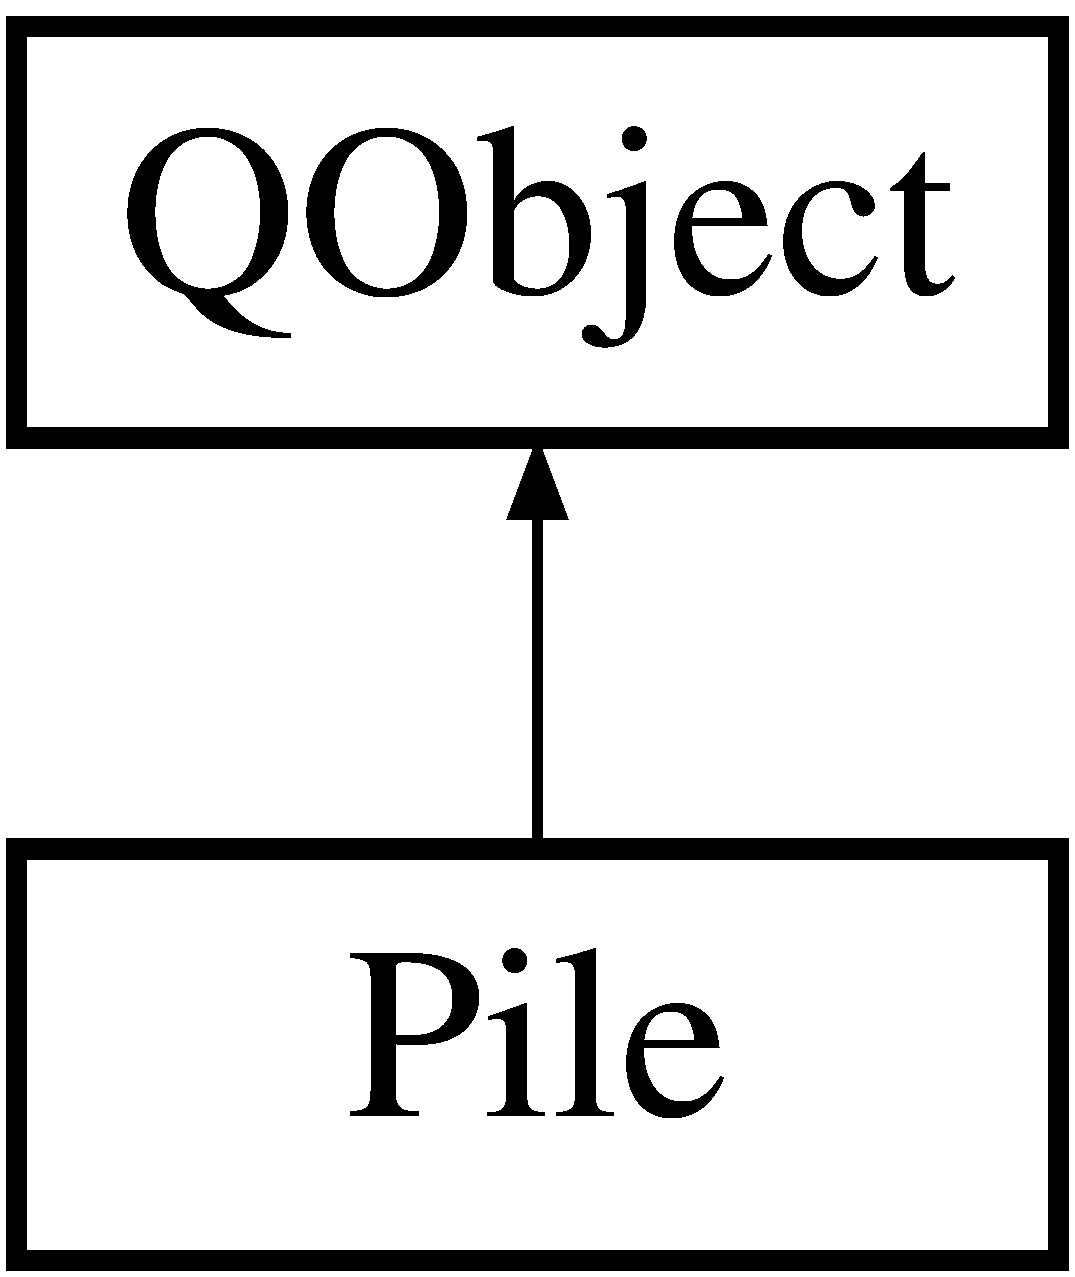
\includegraphics[height=2.000000cm]{class_pile}
\end{center}
\end{figure}
\subsection*{Classes}
\begin{DoxyCompactItemize}
\item 
class \hyperlink{class_pile_1_1iterator}{iterator}
\begin{DoxyCompactList}\small\item\em \hyperlink{class_the}{The} iterator class. \end{DoxyCompactList}\end{DoxyCompactItemize}
\subsection*{Signals}
\begin{DoxyCompactItemize}
\item 
void \hyperlink{class_pile_ac55a0afb626baffd1019567cbaa7f4b2}{modification\+Etat} ()\hypertarget{class_pile_ac55a0afb626baffd1019567cbaa7f4b2}{}\label{class_pile_ac55a0afb626baffd1019567cbaa7f4b2}

\begin{DoxyCompactList}\small\item\em modification\+Etat signal sent when an attribut of the stack is modified \end{DoxyCompactList}\item 
void \hyperlink{class_pile_a9ee28bbf0994bc8f75873b567ba98834}{new\+Message} ()\hypertarget{class_pile_a9ee28bbf0994bc8f75873b567ba98834}{}\label{class_pile_a9ee28bbf0994bc8f75873b567ba98834}

\begin{DoxyCompactList}\small\item\em new\+Messag signal sent when the message of the stack is modified \end{DoxyCompactList}\end{DoxyCompactItemize}
\subsection*{Public Member Functions}
\begin{DoxyCompactItemize}
\item 
\hyperlink{class_pile_ab44e927107b28f5f3ac7697d10e0a739}{Pile} ()
\begin{DoxyCompactList}\small\item\em Constructor. \end{DoxyCompactList}\item 
\hyperlink{class_pile_ab2d1398d675586ff34994e2b109df152}{$\sim$\+Pile} ()
\begin{DoxyCompactList}\small\item\em Destructor. \end{DoxyCompactList}\item 
bool \hyperlink{class_pile_a2ca7edab82a4b7a4305093dd9ab14d71}{est\+Vide} () const 
\begin{DoxyCompactList}\small\item\em \hyperlink{class_pile_a2ca7edab82a4b7a4305093dd9ab14d71}{est\+Vide()} method \end{DoxyCompactList}\item 
unsigned int \hyperlink{class_pile_ac332a47f6d204fe280f199d76893036a}{taille} () const 
\begin{DoxyCompactList}\small\item\em \hyperlink{class_pile_ac332a47f6d204fe280f199d76893036a}{taille()} method \end{DoxyCompactList}\item 
void \hyperlink{class_pile_a874f209b5333810e6179b0061304b4e5}{affiche} () const 
\begin{DoxyCompactList}\small\item\em \hyperlink{class_pile_a874f209b5333810e6179b0061304b4e5}{affiche()} method \end{DoxyCompactList}\item 
void {\bfseries set\+Message} (const Q\+String \&m)\hypertarget{class_pile_adf9495ba02a31d3be1bb8bc5763ec50f}{}\label{class_pile_adf9495ba02a31d3be1bb8bc5763ec50f}

\item 
Q\+String \hyperlink{class_pile_ab04b223738a2fa12b627b138a9c102ed}{get\+Message} () const 
\begin{DoxyCompactList}\small\item\em \hyperlink{class_pile_ab04b223738a2fa12b627b138a9c102ed}{get\+Message()} method \end{DoxyCompactList}\item 
unsigned int \hyperlink{class_pile_acd055c6426813bac9a127c1477c739af}{get\+Nb\+Litterales\+To\+Affiche} () const 
\begin{DoxyCompactList}\small\item\em \hyperlink{class_pile_acd055c6426813bac9a127c1477c739af}{get\+Nb\+Litterales\+To\+Affiche()} method \end{DoxyCompactList}\item 
\hyperlink{class_litterale}{Litterale} $\ast$$\ast$ \hyperlink{class_pile_a6123bd7fb1405c98bf91f3b094a67c2f}{get\+Li} () const 
\begin{DoxyCompactList}\small\item\em \hyperlink{class_pile_a6123bd7fb1405c98bf91f3b094a67c2f}{get\+Li()} method \end{DoxyCompactList}\item 
void \hyperlink{class_pile_a0092075cec9c06331a86c4c9dc12ebca}{set\+Nb\+Litterales\+To\+Affiche} (int n)
\begin{DoxyCompactList}\small\item\em \hyperlink{class_pile_ab04b223738a2fa12b627b138a9c102ed}{get\+Message()} method \end{DoxyCompactList}\item 
void \hyperlink{class_pile_abf3bd33dc3b024dabeda45f020256637}{push} (\hyperlink{class_litterale}{Litterale} $\ast$li)
\begin{DoxyCompactList}\small\item\em \hyperlink{class_pile_abf3bd33dc3b024dabeda45f020256637}{push()} method \end{DoxyCompactList}\item 
\hyperlink{class_litterale}{Litterale} $\ast$ \hyperlink{class_pile_a2321894a738fbfe3a7ffcf55507f567b}{top} () const 
\begin{DoxyCompactList}\small\item\em \hyperlink{class_pile_a2321894a738fbfe3a7ffcf55507f567b}{top()} method \end{DoxyCompactList}\item 
void \hyperlink{class_pile_a081f7843d01cae1f0f7be7d92e46d5d2}{dup} ()
\begin{DoxyCompactList}\small\item\em \hyperlink{class_pile_a081f7843d01cae1f0f7be7d92e46d5d2}{dup()} method \end{DoxyCompactList}\item 
void \hyperlink{class_pile_a7488ed257c6ceb16ed57a9fffb0726d5}{drop} ()
\begin{DoxyCompactList}\small\item\em \hyperlink{class_pile_a7488ed257c6ceb16ed57a9fffb0726d5}{drop()} method \end{DoxyCompactList}\item 
void \hyperlink{class_pile_a2c9967dc8f5dcb4372475dee52ed64c6}{swap} ()
\begin{DoxyCompactList}\small\item\em \hyperlink{class_pile_a2c9967dc8f5dcb4372475dee52ed64c6}{swap()} method \end{DoxyCompactList}\item 
void \hyperlink{class_pile_af91a4b277236024aa5aab9ef410881bb}{undo} ()
\begin{DoxyCompactList}\small\item\em \hyperlink{class_pile_af91a4b277236024aa5aab9ef410881bb}{undo()} method \end{DoxyCompactList}\item 
void \hyperlink{class_pile_aa8319a2921d86236d135cff700a5f833}{redo} ()
\begin{DoxyCompactList}\small\item\em \hyperlink{class_pile_af91a4b277236024aa5aab9ef410881bb}{undo()} method \end{DoxyCompactList}\item 
void \hyperlink{class_pile_aa3991438f190580607d7bbbd50ecc0c3}{clear} ()
\begin{DoxyCompactList}\small\item\em \hyperlink{class_pile_aa3991438f190580607d7bbbd50ecc0c3}{clear()} method \end{DoxyCompactList}\item 
\hyperlink{class_memento}{Memento} $\ast$ \hyperlink{class_pile_a52e78ba1556a05e299926d5a72a48458}{Save\+Stateto\+Memento} ()
\begin{DoxyCompactList}\small\item\em \hyperlink{class_pile_a52e78ba1556a05e299926d5a72a48458}{Save\+Stateto\+Memento()} method. \end{DoxyCompactList}\item 
void \hyperlink{class_pile_a0917465783378b47191cecf459234bc3}{get\+State\+From\+Memento} (\hyperlink{class_memento}{Memento} $\ast$m)
\begin{DoxyCompactList}\small\item\em \hyperlink{class_pile_a0917465783378b47191cecf459234bc3}{get\+State\+From\+Memento()} method \end{DoxyCompactList}\item 
\hyperlink{class_pile_1_1iterator}{iterator} \hyperlink{class_pile_a88900a542fe0be61e8f4da0a601e7924}{begin} ()
\begin{DoxyCompactList}\small\item\em begin to set the iterator at the beginning of the stack \end{DoxyCompactList}\item 
\hyperlink{class_pile_1_1iterator}{iterator} \hyperlink{class_pile_a02e13ab6c7171a3d98a82bf0d908ca07}{end} ()
\begin{DoxyCompactList}\small\item\em end to set the iterator at the end of the stack \end{DoxyCompactList}\end{DoxyCompactItemize}


\subsection{Constructor \& Destructor Documentation}
\index{Pile@{Pile}!Pile@{Pile}}
\index{Pile@{Pile}!Pile@{Pile}}
\subsubsection[{\texorpdfstring{Pile()}{Pile()}}]{\setlength{\rightskip}{0pt plus 5cm}Pile\+::\+Pile (
\begin{DoxyParamCaption}
{}
\end{DoxyParamCaption}
)\hspace{0.3cm}{\ttfamily [inline]}}\hypertarget{class_pile_ab44e927107b28f5f3ac7697d10e0a739}{}\label{class_pile_ab44e927107b28f5f3ac7697d10e0a739}


Constructor. 

Constructor of the \hyperlink{class_pile}{Pile} class Inline Method li, nb, nb\+Max, nb\+Affiche and message are set to 0, and then call of agrandissement\+Capacite()


\begin{DoxyParams}{Parameters}
{\em with} & no parameters \\
\hline
\end{DoxyParams}
\index{Pile@{Pile}!````~Pile@{$\sim$\+Pile}}
\index{````~Pile@{$\sim$\+Pile}!Pile@{Pile}}
\subsubsection[{\texorpdfstring{$\sim$\+Pile()}{~Pile()}}]{\setlength{\rightskip}{0pt plus 5cm}Pile\+::$\sim$\+Pile (
\begin{DoxyParamCaption}
{}
\end{DoxyParamCaption}
)\hspace{0.3cm}{\ttfamily [inline]}}\hypertarget{class_pile_ab2d1398d675586ff34994e2b109df152}{}\label{class_pile_ab2d1398d675586ff34994e2b109df152}


Destructor. 

Destructor of the \hyperlink{class_pile}{Pile} class Inline Method Delete all the elements of the stack and the stack itself, because they are all allocated dynamically


\begin{DoxyParams}{Parameters}
{\em no} & parameters \\
\hline
\end{DoxyParams}


\subsection{Member Function Documentation}
\index{Pile@{Pile}!affiche@{affiche}}
\index{affiche@{affiche}!Pile@{Pile}}
\subsubsection[{\texorpdfstring{affiche() const }{affiche() const }}]{\setlength{\rightskip}{0pt plus 5cm}void Pile\+::affiche (
\begin{DoxyParamCaption}
{}
\end{DoxyParamCaption}
) const}\hypertarget{class_pile_a874f209b5333810e6179b0061304b4e5}{}\label{class_pile_a874f209b5333810e6179b0061304b4e5}


\hyperlink{class_pile_a874f209b5333810e6179b0061304b4e5}{affiche()} method 

Method to print the stack Const Method


\begin{DoxyParams}{Parameters}
{\em no} & parameters \\
\hline
\end{DoxyParams}
\begin{DoxyReturn}{Returns}
void 
\end{DoxyReturn}
\index{Pile@{Pile}!begin@{begin}}
\index{begin@{begin}!Pile@{Pile}}
\subsubsection[{\texorpdfstring{begin()}{begin()}}]{\setlength{\rightskip}{0pt plus 5cm}{\bf iterator} Pile\+::begin (
\begin{DoxyParamCaption}
{}
\end{DoxyParamCaption}
)\hspace{0.3cm}{\ttfamily [inline]}}\hypertarget{class_pile_a88900a542fe0be61e8f4da0a601e7924}{}\label{class_pile_a88900a542fe0be61e8f4da0a601e7924}


begin to set the iterator at the beginning of the stack 

\begin{DoxyReturn}{Returns}
an iterator 
\end{DoxyReturn}
\index{Pile@{Pile}!clear@{clear}}
\index{clear@{clear}!Pile@{Pile}}
\subsubsection[{\texorpdfstring{clear()}{clear()}}]{\setlength{\rightskip}{0pt plus 5cm}void Pile\+::clear (
\begin{DoxyParamCaption}
{}
\end{DoxyParamCaption}
)}\hypertarget{class_pile_aa3991438f190580607d7bbbd50ecc0c3}{}\label{class_pile_aa3991438f190580607d7bbbd50ecc0c3}


\hyperlink{class_pile_aa3991438f190580607d7bbbd50ecc0c3}{clear()} method 

Method to clear the stack of all the \hyperlink{class_litterale}{Litterale} that might be in it (delete them)


\begin{DoxyParams}{Parameters}
{\em no} & parameter \\
\hline
\end{DoxyParams}
\begin{DoxyReturn}{Returns}
void 
\end{DoxyReturn}
\index{Pile@{Pile}!drop@{drop}}
\index{drop@{drop}!Pile@{Pile}}
\subsubsection[{\texorpdfstring{drop()}{drop()}}]{\setlength{\rightskip}{0pt plus 5cm}void Pile\+::drop (
\begin{DoxyParamCaption}
{}
\end{DoxyParamCaption}
)}\hypertarget{class_pile_a7488ed257c6ceb16ed57a9fffb0726d5}{}\label{class_pile_a7488ed257c6ceb16ed57a9fffb0726d5}


\hyperlink{class_pile_a7488ed257c6ceb16ed57a9fffb0726d5}{drop()} method 

Method to delete the element on the top of the stack


\begin{DoxyParams}{Parameters}
{\em no} & parameter \\
\hline
\end{DoxyParams}
\begin{DoxyReturn}{Returns}
void 
\end{DoxyReturn}
\index{Pile@{Pile}!dup@{dup}}
\index{dup@{dup}!Pile@{Pile}}
\subsubsection[{\texorpdfstring{dup()}{dup()}}]{\setlength{\rightskip}{0pt plus 5cm}void Pile\+::dup (
\begin{DoxyParamCaption}
{}
\end{DoxyParamCaption}
)}\hypertarget{class_pile_a081f7843d01cae1f0f7be7d92e46d5d2}{}\label{class_pile_a081f7843d01cae1f0f7be7d92e46d5d2}


\hyperlink{class_pile_a081f7843d01cae1f0f7be7d92e46d5d2}{dup()} method 

Method to duplicate the element on the top of the stack If the stack is full, call of agrandissement\+Capacite()


\begin{DoxyParams}{Parameters}
{\em no} & parameter \\
\hline
\end{DoxyParams}
\begin{DoxyReturn}{Returns}
void 
\end{DoxyReturn}
\index{Pile@{Pile}!end@{end}}
\index{end@{end}!Pile@{Pile}}
\subsubsection[{\texorpdfstring{end()}{end()}}]{\setlength{\rightskip}{0pt plus 5cm}{\bf iterator} Pile\+::end (
\begin{DoxyParamCaption}
{}
\end{DoxyParamCaption}
)\hspace{0.3cm}{\ttfamily [inline]}}\hypertarget{class_pile_a02e13ab6c7171a3d98a82bf0d908ca07}{}\label{class_pile_a02e13ab6c7171a3d98a82bf0d908ca07}


end to set the iterator at the end of the stack 

\begin{DoxyReturn}{Returns}
an iterator 
\end{DoxyReturn}
\index{Pile@{Pile}!est\+Vide@{est\+Vide}}
\index{est\+Vide@{est\+Vide}!Pile@{Pile}}
\subsubsection[{\texorpdfstring{est\+Vide() const }{estVide() const }}]{\setlength{\rightskip}{0pt plus 5cm}bool Pile\+::est\+Vide (
\begin{DoxyParamCaption}
{}
\end{DoxyParamCaption}
) const\hspace{0.3cm}{\ttfamily [inline]}}\hypertarget{class_pile_a2ca7edab82a4b7a4305093dd9ab14d71}{}\label{class_pile_a2ca7edab82a4b7a4305093dd9ab14d71}


\hyperlink{class_pile_a2ca7edab82a4b7a4305093dd9ab14d71}{est\+Vide()} method 

Returns true if the stack is empty Inline const Method


\begin{DoxyParams}{Parameters}
{\em no} & parameters \\
\hline
\end{DoxyParams}
\begin{DoxyReturn}{Returns}
bool 
\end{DoxyReturn}
\index{Pile@{Pile}!get\+Li@{get\+Li}}
\index{get\+Li@{get\+Li}!Pile@{Pile}}
\subsubsection[{\texorpdfstring{get\+Li() const }{getLi() const }}]{\setlength{\rightskip}{0pt plus 5cm}{\bf Litterale}$\ast$$\ast$ Pile\+::get\+Li (
\begin{DoxyParamCaption}
{}
\end{DoxyParamCaption}
) const\hspace{0.3cm}{\ttfamily [inline]}}\hypertarget{class_pile_a6123bd7fb1405c98bf91f3b094a67c2f}{}\label{class_pile_a6123bd7fb1405c98bf91f3b094a67c2f}


\hyperlink{class_pile_a6123bd7fb1405c98bf91f3b094a67c2f}{get\+Li()} method 

Accessor to the message stack itself Inline const Method


\begin{DoxyParams}{Parameters}
{\em no} & parameter \\
\hline
\end{DoxyParams}
\begin{DoxyReturn}{Returns}
Litterale$\ast$$\ast$ 
\end{DoxyReturn}
\index{Pile@{Pile}!get\+Message@{get\+Message}}
\index{get\+Message@{get\+Message}!Pile@{Pile}}
\subsubsection[{\texorpdfstring{get\+Message() const }{getMessage() const }}]{\setlength{\rightskip}{0pt plus 5cm}Q\+String Pile\+::get\+Message (
\begin{DoxyParamCaption}
{}
\end{DoxyParamCaption}
) const\hspace{0.3cm}{\ttfamily [inline]}}\hypertarget{class_pile_ab04b223738a2fa12b627b138a9c102ed}{}\label{class_pile_ab04b223738a2fa12b627b138a9c102ed}


\hyperlink{class_pile_ab04b223738a2fa12b627b138a9c102ed}{get\+Message()} method 

Accessor to the message attribute (of type Q\+String) Inline const Method


\begin{DoxyParams}{Parameters}
{\em no} & parameter \\
\hline
\end{DoxyParams}
\begin{DoxyReturn}{Returns}
Q\+String 
\end{DoxyReturn}
\index{Pile@{Pile}!get\+Nb\+Litterales\+To\+Affiche@{get\+Nb\+Litterales\+To\+Affiche}}
\index{get\+Nb\+Litterales\+To\+Affiche@{get\+Nb\+Litterales\+To\+Affiche}!Pile@{Pile}}
\subsubsection[{\texorpdfstring{get\+Nb\+Litterales\+To\+Affiche() const }{getNbLitteralesToAffiche() const }}]{\setlength{\rightskip}{0pt plus 5cm}unsigned int Pile\+::get\+Nb\+Litterales\+To\+Affiche (
\begin{DoxyParamCaption}
{}
\end{DoxyParamCaption}
) const\hspace{0.3cm}{\ttfamily [inline]}}\hypertarget{class_pile_acd055c6426813bac9a127c1477c739af}{}\label{class_pile_acd055c6426813bac9a127c1477c739af}


\hyperlink{class_pile_acd055c6426813bac9a127c1477c739af}{get\+Nb\+Litterales\+To\+Affiche()} method 

Accessor to the number of element of the stack to display Inline const Method


\begin{DoxyParams}{Parameters}
{\em no} & parameter \\
\hline
\end{DoxyParams}
\begin{DoxyReturn}{Returns}
unsigned int 
\end{DoxyReturn}
\index{Pile@{Pile}!get\+State\+From\+Memento@{get\+State\+From\+Memento}}
\index{get\+State\+From\+Memento@{get\+State\+From\+Memento}!Pile@{Pile}}
\subsubsection[{\texorpdfstring{get\+State\+From\+Memento(\+Memento $\ast$m)}{getStateFromMemento(Memento *m)}}]{\setlength{\rightskip}{0pt plus 5cm}void Pile\+::get\+State\+From\+Memento (
\begin{DoxyParamCaption}
\item[{{\bf Memento} $\ast$}]{m}
\end{DoxyParamCaption}
)\hspace{0.3cm}{\ttfamily [inline]}}\hypertarget{class_pile_a0917465783378b47191cecf459234bc3}{}\label{class_pile_a0917465783378b47191cecf459234bc3}


\hyperlink{class_pile_a0917465783378b47191cecf459234bc3}{get\+State\+From\+Memento()} method 

Method to get back the state of the stack at a T-\/1 moment Make a deep copy of all the Litterales of the stack using Clone() method


\begin{DoxyParams}{Parameters}
{\em m} & \+: a pointer to an object of the class \hyperlink{class_memento}{Memento} \\
\hline
\end{DoxyParams}
\index{Pile@{Pile}!push@{push}}
\index{push@{push}!Pile@{Pile}}
\subsubsection[{\texorpdfstring{push(\+Litterale $\ast$li)}{push(Litterale *li)}}]{\setlength{\rightskip}{0pt plus 5cm}void Pile\+::push (
\begin{DoxyParamCaption}
\item[{{\bf Litterale} $\ast$}]{li}
\end{DoxyParamCaption}
)}\hypertarget{class_pile_abf3bd33dc3b024dabeda45f020256637}{}\label{class_pile_abf3bd33dc3b024dabeda45f020256637}


\hyperlink{class_pile_abf3bd33dc3b024dabeda45f020256637}{push()} method 

Accessor to the add a \hyperlink{class_litterale}{Litterale} to the stack If the stack is full, call of agrandissement\+Capacite()


\begin{DoxyParams}{Parameters}
{\em 1} & parameter of type pointer to \hyperlink{class_litterale}{Litterale} \\
\hline
\end{DoxyParams}
\begin{DoxyReturn}{Returns}
void 
\end{DoxyReturn}
\index{Pile@{Pile}!redo@{redo}}
\index{redo@{redo}!Pile@{Pile}}
\subsubsection[{\texorpdfstring{redo()}{redo()}}]{\setlength{\rightskip}{0pt plus 5cm}void Pile\+::redo (
\begin{DoxyParamCaption}
{}
\end{DoxyParamCaption}
)}\hypertarget{class_pile_aa8319a2921d86236d135cff700a5f833}{}\label{class_pile_aa8319a2921d86236d135cff700a5f833}


\hyperlink{class_pile_af91a4b277236024aa5aab9ef410881bb}{undo()} method 

Method to cancel the action of a redo


\begin{DoxyParams}{Parameters}
{\em no} & parameter \\
\hline
\end{DoxyParams}
\begin{DoxyReturn}{Returns}
void 
\end{DoxyReturn}
\index{Pile@{Pile}!Save\+Stateto\+Memento@{Save\+Stateto\+Memento}}
\index{Save\+Stateto\+Memento@{Save\+Stateto\+Memento}!Pile@{Pile}}
\subsubsection[{\texorpdfstring{Save\+Stateto\+Memento()}{SaveStatetoMemento()}}]{\setlength{\rightskip}{0pt plus 5cm}{\bf Memento}$\ast$ Pile\+::\+Save\+Stateto\+Memento (
\begin{DoxyParamCaption}
{}
\end{DoxyParamCaption}
)\hspace{0.3cm}{\ttfamily [inline]}}\hypertarget{class_pile_a52e78ba1556a05e299926d5a72a48458}{}\label{class_pile_a52e78ba1556a05e299926d5a72a48458}


\hyperlink{class_pile_a52e78ba1556a05e299926d5a72a48458}{Save\+Stateto\+Memento()} method. 

Method to save the state of the pile at a t moment Make a deep copy of all the Litterales of the stack using Clone() method Create a new \hyperlink{class_memento}{Memento}

\begin{DoxyReturn}{Returns}
a pointer to an object of the class \hyperlink{class_memento}{Memento} 
\end{DoxyReturn}
\index{Pile@{Pile}!set\+Nb\+Litterales\+To\+Affiche@{set\+Nb\+Litterales\+To\+Affiche}}
\index{set\+Nb\+Litterales\+To\+Affiche@{set\+Nb\+Litterales\+To\+Affiche}!Pile@{Pile}}
\subsubsection[{\texorpdfstring{set\+Nb\+Litterales\+To\+Affiche(int n)}{setNbLitteralesToAffiche(int n)}}]{\setlength{\rightskip}{0pt plus 5cm}void Pile\+::set\+Nb\+Litterales\+To\+Affiche (
\begin{DoxyParamCaption}
\item[{int}]{n}
\end{DoxyParamCaption}
)\hspace{0.3cm}{\ttfamily [inline]}}\hypertarget{class_pile_a0092075cec9c06331a86c4c9dc12ebca}{}\label{class_pile_a0092075cec9c06331a86c4c9dc12ebca}


\hyperlink{class_pile_ab04b223738a2fa12b627b138a9c102ed}{get\+Message()} method 

Method to set the number of \hyperlink{class_litterale}{Litterale} to display Inline Method


\begin{DoxyParams}{Parameters}
{\em 1} & parameter of type int \\
\hline
\end{DoxyParams}
\begin{DoxyReturn}{Returns}
void 
\end{DoxyReturn}
\index{Pile@{Pile}!swap@{swap}}
\index{swap@{swap}!Pile@{Pile}}
\subsubsection[{\texorpdfstring{swap()}{swap()}}]{\setlength{\rightskip}{0pt plus 5cm}void Pile\+::swap (
\begin{DoxyParamCaption}
{}
\end{DoxyParamCaption}
)}\hypertarget{class_pile_a2c9967dc8f5dcb4372475dee52ed64c6}{}\label{class_pile_a2c9967dc8f5dcb4372475dee52ed64c6}


\hyperlink{class_pile_a2c9967dc8f5dcb4372475dee52ed64c6}{swap()} method 

Method to swap the 2 elements on the top of the stack


\begin{DoxyParams}{Parameters}
{\em no} & parameter \\
\hline
\end{DoxyParams}
\begin{DoxyReturn}{Returns}
void 
\end{DoxyReturn}
\index{Pile@{Pile}!taille@{taille}}
\index{taille@{taille}!Pile@{Pile}}
\subsubsection[{\texorpdfstring{taille() const }{taille() const }}]{\setlength{\rightskip}{0pt plus 5cm}unsigned int Pile\+::taille (
\begin{DoxyParamCaption}
{}
\end{DoxyParamCaption}
) const\hspace{0.3cm}{\ttfamily [inline]}}\hypertarget{class_pile_ac332a47f6d204fe280f199d76893036a}{}\label{class_pile_ac332a47f6d204fe280f199d76893036a}


\hyperlink{class_pile_ac332a47f6d204fe280f199d76893036a}{taille()} method 

Accessor to the size of the stack Inline const Method


\begin{DoxyParams}{Parameters}
{\em no} & parameters \\
\hline
\end{DoxyParams}
\begin{DoxyReturn}{Returns}
unsigned int 
\end{DoxyReturn}
\index{Pile@{Pile}!top@{top}}
\index{top@{top}!Pile@{Pile}}
\subsubsection[{\texorpdfstring{top() const }{top() const }}]{\setlength{\rightskip}{0pt plus 5cm}{\bf Litterale} $\ast$ Pile\+::top (
\begin{DoxyParamCaption}
{}
\end{DoxyParamCaption}
) const}\hypertarget{class_pile_a2321894a738fbfe3a7ffcf55507f567b}{}\label{class_pile_a2321894a738fbfe3a7ffcf55507f567b}


\hyperlink{class_pile_a2321894a738fbfe3a7ffcf55507f567b}{top()} method 

Accessor to the element on the top of the stack Const Method


\begin{DoxyParams}{Parameters}
{\em no} & parameter \\
\hline
\end{DoxyParams}
\begin{DoxyReturn}{Returns}
Litterale$\ast$ 
\end{DoxyReturn}
\index{Pile@{Pile}!undo@{undo}}
\index{undo@{undo}!Pile@{Pile}}
\subsubsection[{\texorpdfstring{undo()}{undo()}}]{\setlength{\rightskip}{0pt plus 5cm}void Pile\+::undo (
\begin{DoxyParamCaption}
{}
\end{DoxyParamCaption}
)}\hypertarget{class_pile_af91a4b277236024aa5aab9ef410881bb}{}\label{class_pile_af91a4b277236024aa5aab9ef410881bb}


\hyperlink{class_pile_af91a4b277236024aa5aab9ef410881bb}{undo()} method 

Method to reset the state of the stack before the last operation


\begin{DoxyParams}{Parameters}
{\em no} & parameter \\
\hline
\end{DoxyParams}
\begin{DoxyReturn}{Returns}
void 
\end{DoxyReturn}


The documentation for this class was generated from the following files\+:\begin{DoxyCompactItemize}
\item 
\hyperlink{pile_8h}{pile.\+h}\item 
\hyperlink{pile_8cpp}{pile.\+cpp}\end{DoxyCompactItemize}

\hypertarget{class_the}{}\section{The Class Reference}
\label{class_the}\index{The@{The}}


Class to manage the calculator.  




\subsection{Detailed Description}
Class to manage the calculator. 

Class to contain all the \hyperlink{class_litterale}{Litterale} of the calculator.

Class to save the attributes of a pile at a T moment.

Abstract class from which inherits all the other litterale class (\hyperlink{class_li_numerique}{Li\+Numerique} and \hyperlink{class_li_complexe}{Li\+Complexe})

abstract class which inherits from the abstract class \hyperlink{class_litterale}{Litterale}

Class which inherits from \hyperlink{class_litterale}{Litterale}.

class to manage all the exception of the calculator

Class which inherits from \hyperlink{class_li_numerique}{Li\+Numerique}.

2 attributes of type pointer to \hyperlink{class_li_numerique}{Li\+Numerique}. \hyperlink{class_the}{The} real and the imaginary part of a \hyperlink{class_li_complexe}{Li\+Complexe} can either be a \hyperlink{class_li_entiere}{Li\+Entiere}, a \hyperlink{class_li_reelle}{Li\+Reelle} or a \hyperlink{class_li_rationnelle}{Li\+Rationnelle}. used to represent the complexe objects in the calculator.

1 attribut of type int called value used to represent the integers in the Calculator

All the exception are send to this class

Used to represent all the expression in the Calculator

used to define li\+Entiere, \hyperlink{class_li_reelle}{Li\+Reelle} and \hyperlink{class_li_rationnelle}{Li\+Rationnelle} no attributes

2 attributs of type \hyperlink{class_li_entiere}{Li\+Entiere} used to represent the rationnal numbers in the calculator

1 attribut of type double used to represent the real numbers (nombres à virgule) in the calculator

No attributes but pure virtual methods which will be defined in the inherited classes 

The documentation for this class was generated from the following file\+:\begin{DoxyCompactItemize}
\item 
\hyperlink{calculatrice_8h}{calculatrice.\+h}\end{DoxyCompactItemize}

\chapter{File Documentation}
\hypertarget{calculatrice_8cpp}{}\section{calculatrice.\+cpp File Reference}
\label{calculatrice_8cpp}\index{calculatrice.\+cpp@{calculatrice.\+cpp}}


file where the methods of the \hyperlink{class_calculatrice}{Calculatrice} class are defined  


{\ttfamily \#include \char`\"{}calculatrice.\+h\char`\"{}}\\*
Include dependency graph for calculatrice.\+cpp\+:

\hypertarget{calculatrice_8h}{}\section{calculatrice.\+h File Reference}
\label{calculatrice_8h}\index{calculatrice.\+h@{calculatrice.\+h}}


file where the class \hyperlink{class_calculatrice}{Calculatrice} is defined  


{\ttfamily \#include \char`\"{}pile.\+h\char`\"{}}\\*
\subsection*{Classes}
\begin{DoxyCompactItemize}
\item 
class \hyperlink{class_calculatrice}{Calculatrice}
\end{DoxyCompactItemize}
\subsection*{Functions}
\begin{DoxyCompactItemize}
\item 
bool \hyperlink{calculatrice_8h_a6ae3100d316a03f46973ad326c11f038}{est\+Un\+Operateur\+Binaire} (const Q\+String \&s)
\begin{DoxyCompactList}\small\item\em \hyperlink{calculatrice_8h_a6ae3100d316a03f46973ad326c11f038}{est\+Un\+Operateur\+Binaire()} method \end{DoxyCompactList}\item 
bool \hyperlink{calculatrice_8h_aaa1ac3d006923b4d0cf4bc99aa43c1f3}{est\+Un\+Operateur\+De\+Pile} (const Q\+String \&s)
\begin{DoxyCompactList}\small\item\em est\+Un\+Operateur\+Unaire() method \end{DoxyCompactList}\item 
bool \hyperlink{calculatrice_8h_a1c8a6de19df58bdd91993528eb54944e}{est\+Entier} (const Q\+String \&s)
\begin{DoxyCompactList}\small\item\em \hyperlink{calculatrice_8h_a1c8a6de19df58bdd91993528eb54944e}{est\+Entier()} method \end{DoxyCompactList}\item 
bool \hyperlink{calculatrice_8h_a8fb667d9e02a9ff4127bada083433de0}{est\+Double} (const Q\+String \&s)
\begin{DoxyCompactList}\small\item\em \hyperlink{calculatrice_8h_a8fb667d9e02a9ff4127bada083433de0}{est\+Double()} method \end{DoxyCompactList}\item 
bool \hyperlink{calculatrice_8h_aa2ab97d82a097fc21f182826172d0e61}{est\+Expression} (const Q\+String \&s)
\begin{DoxyCompactList}\small\item\em \hyperlink{calculatrice_8h_aa2ab97d82a097fc21f182826172d0e61}{est\+Expression()} method \end{DoxyCompactList}\item 
bool \hyperlink{calculatrice_8h_a76c3d1b85beb68eaa390fd356d07f1d8}{est\+Atome\+Guillemets} (const Q\+String \&s)
\begin{DoxyCompactList}\small\item\em \hyperlink{calculatrice_8h_a76c3d1b85beb68eaa390fd356d07f1d8}{est\+Atome\+Guillemets()} method \end{DoxyCompactList}\item 
bool \hyperlink{calculatrice_8h_ae70d9e7f492982ade1d91c5071c9a3d8}{est\+Atome} (const Q\+String \&s)
\begin{DoxyCompactList}\small\item\em \hyperlink{calculatrice_8h_ae70d9e7f492982ade1d91c5071c9a3d8}{est\+Atome()} method \end{DoxyCompactList}\item 
bool {\bfseries is1operator} (const Q\+String \&s)\hypertarget{calculatrice_8h_a4a20a4deccf548a7c6b4217ae50a2efc}{}\label{calculatrice_8h_a4a20a4deccf548a7c6b4217ae50a2efc}

\item 
bool {\bfseries is2operator} (const Q\+String \&s)\hypertarget{calculatrice_8h_aeb7fd694744ba8368072dc46c752abef}{}\label{calculatrice_8h_aeb7fd694744ba8368072dc46c752abef}

\item 
bool \hyperlink{calculatrice_8h_aaa5f2850c69dfe13da6cb3ba27c1e98c}{is1operator\+PP} (const Q\+String \&s)
\begin{DoxyCompactList}\small\item\em \hyperlink{calculatrice_8h_a76c3d1b85beb68eaa390fd356d07f1d8}{est\+Atome\+Guillemets()} method \end{DoxyCompactList}\item 
bool \hyperlink{calculatrice_8h_a639cddd004cb2a26b6b52962cf668f98}{is2operator\+P\+VP} (const Q\+String \&s)
\begin{DoxyCompactList}\small\item\em \hyperlink{calculatrice_8h_a76c3d1b85beb68eaa390fd356d07f1d8}{est\+Atome\+Guillemets()} method \end{DoxyCompactList}\item 
bool \hyperlink{calculatrice_8h_a67c2112828c3f10d1d9d64cf756a47b1}{Priorite\+Precedent\+Sup} (const Q\+Char qc, const Q\+Char ptop)
\begin{DoxyCompactList}\small\item\em \hyperlink{calculatrice_8h_a76c3d1b85beb68eaa390fd356d07f1d8}{est\+Atome\+Guillemets()} method \end{DoxyCompactList}\item 
int \hyperlink{calculatrice_8h_a853a007dad172b583f23c1570f16b02e}{priorite\+Op} (const Q\+String \&s)
\begin{DoxyCompactList}\small\item\em \hyperlink{calculatrice_8h_a76c3d1b85beb68eaa390fd356d07f1d8}{est\+Atome\+Guillemets()} method \end{DoxyCompactList}\end{DoxyCompactItemize}


\subsection{Detailed Description}
file where the class \hyperlink{class_calculatrice}{Calculatrice} is defined 

\begin{DoxyAuthor}{Author}
Virgile V\+A\+N\+C\+ON and Nicolas M\+A\+R\+C\+A\+D\+ET 
\end{DoxyAuthor}
\begin{DoxyVersion}{Version}
0.\+1 
\end{DoxyVersion}
\begin{DoxyDate}{Date}
12 Juin 2016 
\end{DoxyDate}


\subsection{Function Documentation}
\index{calculatrice.\+h@{calculatrice.\+h}!est\+Atome@{est\+Atome}}
\index{est\+Atome@{est\+Atome}!calculatrice.\+h@{calculatrice.\+h}}
\subsubsection[{\texorpdfstring{est\+Atome(const Q\+String \&s)}{estAtome(const QString &s)}}]{\setlength{\rightskip}{0pt plus 5cm}bool est\+Atome (
\begin{DoxyParamCaption}
\item[{const Q\+String \&}]{s}
\end{DoxyParamCaption}
)}\hypertarget{calculatrice_8h_ae70d9e7f492982ade1d91c5071c9a3d8}{}\label{calculatrice_8h_ae70d9e7f492982ade1d91c5071c9a3d8}


\hyperlink{calculatrice_8h_ae70d9e7f492982ade1d91c5071c9a3d8}{est\+Atome()} method 

Method used to know if a Q\+String is an atome without quotes Use regular expressions


\begin{DoxyParams}{Parameters}
{\em const} & Q\+String\& s \\
\hline
\end{DoxyParams}
\begin{DoxyReturn}{Returns}
bool 
\end{DoxyReturn}
\index{calculatrice.\+h@{calculatrice.\+h}!est\+Atome\+Guillemets@{est\+Atome\+Guillemets}}
\index{est\+Atome\+Guillemets@{est\+Atome\+Guillemets}!calculatrice.\+h@{calculatrice.\+h}}
\subsubsection[{\texorpdfstring{est\+Atome\+Guillemets(const Q\+String \&s)}{estAtomeGuillemets(const QString &s)}}]{\setlength{\rightskip}{0pt plus 5cm}bool est\+Atome\+Guillemets (
\begin{DoxyParamCaption}
\item[{const Q\+String \&}]{s}
\end{DoxyParamCaption}
)}\hypertarget{calculatrice_8h_a76c3d1b85beb68eaa390fd356d07f1d8}{}\label{calculatrice_8h_a76c3d1b85beb68eaa390fd356d07f1d8}


\hyperlink{calculatrice_8h_a76c3d1b85beb68eaa390fd356d07f1d8}{est\+Atome\+Guillemets()} method 

Method used to know if a Q\+String is an atome with quotes Use regular expressions


\begin{DoxyParams}{Parameters}
{\em const} & Q\+String\& s \\
\hline
\end{DoxyParams}
\begin{DoxyReturn}{Returns}
bool 
\end{DoxyReturn}
\index{calculatrice.\+h@{calculatrice.\+h}!est\+Double@{est\+Double}}
\index{est\+Double@{est\+Double}!calculatrice.\+h@{calculatrice.\+h}}
\subsubsection[{\texorpdfstring{est\+Double(const Q\+String \&s)}{estDouble(const QString &s)}}]{\setlength{\rightskip}{0pt plus 5cm}bool est\+Double (
\begin{DoxyParamCaption}
\item[{const Q\+String \&}]{s}
\end{DoxyParamCaption}
)}\hypertarget{calculatrice_8h_a8fb667d9e02a9ff4127bada083433de0}{}\label{calculatrice_8h_a8fb667d9e02a9ff4127bada083433de0}


\hyperlink{calculatrice_8h_a8fb667d9e02a9ff4127bada083433de0}{est\+Double()} method 

Method used to know if a Q\+String is an double Use regular expressions


\begin{DoxyParams}{Parameters}
{\em const} & Q\+String\& s \\
\hline
\end{DoxyParams}
\begin{DoxyReturn}{Returns}
bool 
\end{DoxyReturn}
\index{calculatrice.\+h@{calculatrice.\+h}!est\+Entier@{est\+Entier}}
\index{est\+Entier@{est\+Entier}!calculatrice.\+h@{calculatrice.\+h}}
\subsubsection[{\texorpdfstring{est\+Entier(const Q\+String \&s)}{estEntier(const QString &s)}}]{\setlength{\rightskip}{0pt plus 5cm}bool est\+Entier (
\begin{DoxyParamCaption}
\item[{const Q\+String \&}]{s}
\end{DoxyParamCaption}
)}\hypertarget{calculatrice_8h_a1c8a6de19df58bdd91993528eb54944e}{}\label{calculatrice_8h_a1c8a6de19df58bdd91993528eb54944e}


\hyperlink{calculatrice_8h_a1c8a6de19df58bdd91993528eb54944e}{est\+Entier()} method 

Method used to know if a Q\+String is an integer Use regular expressions


\begin{DoxyParams}{Parameters}
{\em const} & Q\+String\& s \\
\hline
\end{DoxyParams}
\begin{DoxyReturn}{Returns}
bool 
\end{DoxyReturn}
\index{calculatrice.\+h@{calculatrice.\+h}!est\+Expression@{est\+Expression}}
\index{est\+Expression@{est\+Expression}!calculatrice.\+h@{calculatrice.\+h}}
\subsubsection[{\texorpdfstring{est\+Expression(const Q\+String \&s)}{estExpression(const QString &s)}}]{\setlength{\rightskip}{0pt plus 5cm}bool est\+Expression (
\begin{DoxyParamCaption}
\item[{const Q\+String \&}]{s}
\end{DoxyParamCaption}
)}\hypertarget{calculatrice_8h_aa2ab97d82a097fc21f182826172d0e61}{}\label{calculatrice_8h_aa2ab97d82a097fc21f182826172d0e61}


\hyperlink{calculatrice_8h_aa2ab97d82a097fc21f182826172d0e61}{est\+Expression()} method 

Method used to know if a Q\+String is an Expression Use regular expressions


\begin{DoxyParams}{Parameters}
{\em const} & Q\+String\& s \\
\hline
\end{DoxyParams}
\begin{DoxyReturn}{Returns}
bool 
\end{DoxyReturn}
\index{calculatrice.\+h@{calculatrice.\+h}!est\+Un\+Operateur\+Binaire@{est\+Un\+Operateur\+Binaire}}
\index{est\+Un\+Operateur\+Binaire@{est\+Un\+Operateur\+Binaire}!calculatrice.\+h@{calculatrice.\+h}}
\subsubsection[{\texorpdfstring{est\+Un\+Operateur\+Binaire(const Q\+String \&s)}{estUnOperateurBinaire(const QString &s)}}]{\setlength{\rightskip}{0pt plus 5cm}bool est\+Un\+Operateur\+Binaire (
\begin{DoxyParamCaption}
\item[{const Q\+String \&}]{s}
\end{DoxyParamCaption}
)}\hypertarget{calculatrice_8h_a6ae3100d316a03f46973ad326c11f038}{}\label{calculatrice_8h_a6ae3100d316a03f46973ad326c11f038}


\hyperlink{calculatrice_8h_a6ae3100d316a03f46973ad326c11f038}{est\+Un\+Operateur\+Binaire()} method 

Method used to know if a Q\+String is a binary operator


\begin{DoxyParams}{Parameters}
{\em const} & Q\+String\& s \\
\hline
\end{DoxyParams}
\begin{DoxyReturn}{Returns}
bool 
\end{DoxyReturn}
\index{calculatrice.\+h@{calculatrice.\+h}!est\+Un\+Operateur\+De\+Pile@{est\+Un\+Operateur\+De\+Pile}}
\index{est\+Un\+Operateur\+De\+Pile@{est\+Un\+Operateur\+De\+Pile}!calculatrice.\+h@{calculatrice.\+h}}
\subsubsection[{\texorpdfstring{est\+Un\+Operateur\+De\+Pile(const Q\+String \&s)}{estUnOperateurDePile(const QString &s)}}]{\setlength{\rightskip}{0pt plus 5cm}bool est\+Un\+Operateur\+De\+Pile (
\begin{DoxyParamCaption}
\item[{const Q\+String \&}]{s}
\end{DoxyParamCaption}
)}\hypertarget{calculatrice_8h_aaa1ac3d006923b4d0cf4bc99aa43c1f3}{}\label{calculatrice_8h_aaa1ac3d006923b4d0cf4bc99aa43c1f3}


est\+Un\+Operateur\+Unaire() method 

operateur2() method

Method used to know if a Q\+String is a unaire operator


\begin{DoxyParams}{Parameters}
{\em const} & Q\+String\& s \\
\hline
\end{DoxyParams}
\begin{DoxyReturn}{Returns}
bool
\end{DoxyReturn}
Method used to know if a Q\+String is a stack operator


\begin{DoxyParams}{Parameters}
{\em const} & Q\+String\& s \\
\hline
\end{DoxyParams}
\begin{DoxyReturn}{Returns}
bool
\end{DoxyReturn}
est\+Un\+Operateur\+Unaire() method

Method used to know if a Q\+String is a stack operator


\begin{DoxyParams}{Parameters}
{\em const} & Q\+String\& s \\
\hline
\end{DoxyParams}
\begin{DoxyReturn}{Returns}
bool 
\end{DoxyReturn}
\index{calculatrice.\+h@{calculatrice.\+h}!is1operator\+PP@{is1operator\+PP}}
\index{is1operator\+PP@{is1operator\+PP}!calculatrice.\+h@{calculatrice.\+h}}
\subsubsection[{\texorpdfstring{is1operator\+P\+P(const Q\+String \&s)}{is1operatorPP(const QString &s)}}]{\setlength{\rightskip}{0pt plus 5cm}bool is1operator\+PP (
\begin{DoxyParamCaption}
\item[{const Q\+String \&}]{s}
\end{DoxyParamCaption}
)}\hypertarget{calculatrice_8h_aaa5f2850c69dfe13da6cb3ba27c1e98c}{}\label{calculatrice_8h_aaa5f2850c69dfe13da6cb3ba27c1e98c}


\hyperlink{calculatrice_8h_a76c3d1b85beb68eaa390fd356d07f1d8}{est\+Atome\+Guillemets()} method 

Method used to know if a of the type OP(...)


\begin{DoxyParams}{Parameters}
{\em const} & Q\+String\& s \\
\hline
\end{DoxyParams}
\begin{DoxyReturn}{Returns}
bool 
\end{DoxyReturn}
\index{calculatrice.\+h@{calculatrice.\+h}!is2operator\+P\+VP@{is2operator\+P\+VP}}
\index{is2operator\+P\+VP@{is2operator\+P\+VP}!calculatrice.\+h@{calculatrice.\+h}}
\subsubsection[{\texorpdfstring{is2operator\+P\+V\+P(const Q\+String \&s)}{is2operatorPVP(const QString &s)}}]{\setlength{\rightskip}{0pt plus 5cm}bool is2operator\+P\+VP (
\begin{DoxyParamCaption}
\item[{const Q\+String \&}]{s}
\end{DoxyParamCaption}
)}\hypertarget{calculatrice_8h_a639cddd004cb2a26b6b52962cf668f98}{}\label{calculatrice_8h_a639cddd004cb2a26b6b52962cf668f98}


\hyperlink{calculatrice_8h_a76c3d1b85beb68eaa390fd356d07f1d8}{est\+Atome\+Guillemets()} method 

Method used to know if a of the type OP(..., ...)


\begin{DoxyParams}{Parameters}
{\em const} & Q\+String\& s \\
\hline
\end{DoxyParams}
\begin{DoxyReturn}{Returns}
bool 
\end{DoxyReturn}
\index{calculatrice.\+h@{calculatrice.\+h}!priorite\+Op@{priorite\+Op}}
\index{priorite\+Op@{priorite\+Op}!calculatrice.\+h@{calculatrice.\+h}}
\subsubsection[{\texorpdfstring{priorite\+Op(const Q\+String \&s)}{prioriteOp(const QString &s)}}]{\setlength{\rightskip}{0pt plus 5cm}int priorite\+Op (
\begin{DoxyParamCaption}
\item[{const Q\+String \&}]{s}
\end{DoxyParamCaption}
)}\hypertarget{calculatrice_8h_a853a007dad172b583f23c1570f16b02e}{}\label{calculatrice_8h_a853a007dad172b583f23c1570f16b02e}


\hyperlink{calculatrice_8h_a76c3d1b85beb68eaa390fd356d07f1d8}{est\+Atome\+Guillemets()} method 

Method used to know the priority of an operator Throws an error if the parameter is not an operator


\begin{DoxyParams}{Parameters}
{\em const} & Q\+String\& s \\
\hline
\end{DoxyParams}
\begin{DoxyReturn}{Returns}
int 
\end{DoxyReturn}
\index{calculatrice.\+h@{calculatrice.\+h}!Priorite\+Precedent\+Sup@{Priorite\+Precedent\+Sup}}
\index{Priorite\+Precedent\+Sup@{Priorite\+Precedent\+Sup}!calculatrice.\+h@{calculatrice.\+h}}
\subsubsection[{\texorpdfstring{Priorite\+Precedent\+Sup(const Q\+Char qc, const Q\+Char ptop)}{PrioritePrecedentSup(const QChar qc, const QChar ptop)}}]{\setlength{\rightskip}{0pt plus 5cm}bool Priorite\+Precedent\+Sup (
\begin{DoxyParamCaption}
\item[{const Q\+Char}]{qc, }
\item[{const Q\+Char}]{ptop}
\end{DoxyParamCaption}
)}\hypertarget{calculatrice_8h_a67c2112828c3f10d1d9d64cf756a47b1}{}\label{calculatrice_8h_a67c2112828c3f10d1d9d64cf756a47b1}


\hyperlink{calculatrice_8h_a76c3d1b85beb68eaa390fd356d07f1d8}{est\+Atome\+Guillemets()} method 

Method used to know if the priority of the operator ptop is higher than the priority of the operator qc


\begin{DoxyParams}{Parameters}
{\em const} & Q\+String\& s \\
\hline
\end{DoxyParams}
\begin{DoxyReturn}{Returns}
bool 
\end{DoxyReturn}

\hypertarget{licomplexe_8cpp}{}\section{licomplexe.\+cpp File Reference}
\label{licomplexe_8cpp}\index{licomplexe.\+cpp@{licomplexe.\+cpp}}


file where the methods of the \hyperlink{class_li_complexe}{Li\+Complexe} class are defined  


{\ttfamily \#include \char`\"{}liexpression.\+h\char`\"{}}\\*
Include dependency graph for licomplexe.\+cpp\+:
% FIG 0


\subsection{Detailed Description}
file where the methods of the \hyperlink{class_li_complexe}{Li\+Complexe} class are defined 

\begin{DoxyAuthor}{Author}
Virgile V\+A\+N\+C\+ON and Nicolas M\+A\+R\+C\+A\+D\+ET 
\end{DoxyAuthor}
\begin{DoxyVersion}{Version}
0.\+1 
\end{DoxyVersion}
\begin{DoxyDate}{Date}
12 Juin 2016 
\end{DoxyDate}

\hypertarget{licomplexe_8h}{}\section{licomplexe.\+h File Reference}
\label{licomplexe_8h}\index{licomplexe.\+h@{licomplexe.\+h}}


file where the class \hyperlink{class_li_complexe}{Li\+Complexe} is defined  


{\ttfamily \#include \char`\"{}lirationnelle.\+h\char`\"{}}\\*
Include dependency graph for licomplexe.\+h\+:
% FIG 0
This graph shows which files directly or indirectly include this file\+:
% FIG 1
\subsection*{Classes}
\begin{DoxyCompactItemize}
\item 
class \hyperlink{class_li_complexe}{Li\+Complexe}
\end{DoxyCompactItemize}


\subsection{Detailed Description}
file where the class \hyperlink{class_li_complexe}{Li\+Complexe} is defined 

\begin{DoxyAuthor}{Author}
Virgile V\+A\+N\+C\+ON and Nicolas M\+A\+R\+C\+A\+D\+ET 
\end{DoxyAuthor}
\begin{DoxyVersion}{Version}
0.\+1 
\end{DoxyVersion}
\begin{DoxyDate}{Date}
12 Juin 2016 
\end{DoxyDate}

\hypertarget{lientiere_8cpp}{}\section{lientiere.\+cpp File Reference}
\label{lientiere_8cpp}\index{lientiere.\+cpp@{lientiere.\+cpp}}


file where the methods of the \hyperlink{class_li_entiere}{Li\+Entiere} class are defined  


{\ttfamily \#include \char`\"{}liexpression.\+h\char`\"{}}\\*
Include dependency graph for lientiere.\+cpp\+:
% FIG 0


\subsection{Detailed Description}
file where the methods of the \hyperlink{class_li_entiere}{Li\+Entiere} class are defined 

\begin{DoxyAuthor}{Author}
Virgile V\+A\+N\+C\+ON and Nicolas M\+A\+R\+C\+A\+D\+ET 
\end{DoxyAuthor}
\begin{DoxyVersion}{Version}
0.\+1 
\end{DoxyVersion}
\begin{DoxyDate}{Date}
12 Juin 2016 
\end{DoxyDate}

\hypertarget{lientiere_8h}{}\section{lientiere.\+h File Reference}
\label{lientiere_8h}\index{lientiere.\+h@{lientiere.\+h}}


file where the class \hyperlink{class_li_entiere}{Li\+Entiere} is defined  


{\ttfamily \#include \char`\"{}linumerique.\+h\char`\"{}}\\*
Include dependency graph for lientiere.\+h\+:
% FIG 0
This graph shows which files directly or indirectly include this file\+:
% FIG 1
\subsection*{Classes}
\begin{DoxyCompactItemize}
\item 
class \hyperlink{class_li_entiere}{Li\+Entiere}
\end{DoxyCompactItemize}


\subsection{Detailed Description}
file where the class \hyperlink{class_li_entiere}{Li\+Entiere} is defined 

\begin{DoxyAuthor}{Author}
Virgile V\+A\+N\+C\+ON and Nicolas M\+A\+R\+C\+A\+D\+ET 
\end{DoxyAuthor}
\begin{DoxyVersion}{Version}
0.\+1 
\end{DoxyVersion}
\begin{DoxyDate}{Date}
12 Juin 2016 
\end{DoxyDate}

\hypertarget{liexception_8h}{}\section{liexception.\+h File Reference}
\label{liexception_8h}\index{liexception.\+h@{liexception.\+h}}


file where the class managing the exception is defined  


{\ttfamily \#include $<$iostream$>$}\\*
{\ttfamily \#include $<$stdio.\+h$>$}\\*
{\ttfamily \#include $<$string.\+h$>$}\\*
{\ttfamily \#include $<$string$>$}\\*
{\ttfamily \#include $<$math.\+h$>$}\\*
{\ttfamily \#include $<$typeinfo$>$}\\*
{\ttfamily \#include $<$sstream$>$}\\*
{\ttfamily \#include $<$cstdlib$>$}\\*
{\ttfamily \#include $<$Q\+String$>$}\\*
{\ttfamily \#include $<$Q\+String\+Builder$>$}\\*
{\ttfamily \#include $<$Q\+Text\+Stream$>$}\\*
{\ttfamily \#include $<$Q\+Main\+Window$>$}\\*
{\ttfamily \#include $<$Q\+Debug$>$}\\*
{\ttfamily \#include $<$Q\+Widget$>$}\\*
{\ttfamily \#include $<$Q\+Line\+Edit$>$}\\*
{\ttfamily \#include $<$Q\+Key\+Event$>$}\\*
{\ttfamily \#include $<$Q\+Table\+Widget$>$}\\*
{\ttfamily \#include $<$Q\+Regexp$>$}\\*
{\ttfamily \#include $<$Q\+Stack$>$}\\*
{\ttfamily \#include $<$Map$>$}\\*
{\ttfamily \#include $<$Q\+Combo\+Box$>$}\\*
Include dependency graph for liexception.\+h\+:
% FIG 0
This graph shows which files directly or indirectly include this file\+:
% FIG 1
\subsection*{Classes}
\begin{DoxyCompactItemize}
\item 
class \hyperlink{class_li_exception}{Li\+Exception}
\end{DoxyCompactItemize}


\subsection{Detailed Description}
file where the class managing the exception is defined 

\begin{DoxyAuthor}{Author}
Virgile V\+A\+N\+C\+ON and Nicolas M\+A\+R\+C\+A\+D\+ET 
\end{DoxyAuthor}
\begin{DoxyVersion}{Version}
0.\+1 
\end{DoxyVersion}
\begin{DoxyDate}{Date}
12 Juin 2016 
\end{DoxyDate}

\hypertarget{liexpression_8cpp}{}\section{liexpression.\+cpp File Reference}
\label{liexpression_8cpp}\index{liexpression.\+cpp@{liexpression.\+cpp}}


file where the methods of the \hyperlink{class_li_expression}{Li\+Expression} class are defined  


{\ttfamily \#include \char`\"{}liexpression.\+h\char`\"{}}\\*
Include dependency graph for liexpression.\+cpp\+:
% FIG 0


\subsection{Detailed Description}
file where the methods of the \hyperlink{class_li_expression}{Li\+Expression} class are defined 

\begin{DoxyAuthor}{Author}
Virgile V\+A\+N\+C\+ON and Nicolas M\+A\+R\+C\+A\+D\+ET 
\end{DoxyAuthor}
\begin{DoxyVersion}{Version}
0.\+1 
\end{DoxyVersion}
\begin{DoxyDate}{Date}
12 Juin 2016 
\end{DoxyDate}

\hypertarget{liexpression_8h}{}\section{liexpression.\+h File Reference}
\label{liexpression_8h}\index{liexpression.\+h@{liexpression.\+h}}


file where the class \hyperlink{class_li_expression}{Li\+Expression} is defined  


{\ttfamily \#include \char`\"{}licomplexe.\+h\char`\"{}}\\*
Include dependency graph for liexpression.\+h\+:
% FIG 0
This graph shows which files directly or indirectly include this file\+:
% FIG 1
\subsection*{Classes}
\begin{DoxyCompactItemize}
\item 
class \hyperlink{class_li_expression}{Li\+Expression}
\end{DoxyCompactItemize}


\subsection{Detailed Description}
file where the class \hyperlink{class_li_expression}{Li\+Expression} is defined 

\begin{DoxyAuthor}{Author}
Virgile V\+A\+N\+C\+ON and Nicolas M\+A\+R\+C\+A\+D\+ET 
\end{DoxyAuthor}
\begin{DoxyVersion}{Version}
0.\+1 
\end{DoxyVersion}
\begin{DoxyDate}{Date}
12 Juin 2016 
\end{DoxyDate}

\hypertarget{linumerique_8h}{}\section{linumerique.\+h File Reference}
\label{linumerique_8h}\index{linumerique.\+h@{linumerique.\+h}}


file where the class \hyperlink{class_li_numerique}{Li\+Numerique} is defined  


{\ttfamily \#include \char`\"{}litterale.\+h\char`\"{}}\\*
Include dependency graph for linumerique.\+h\+:
% FIG 0
This graph shows which files directly or indirectly include this file\+:
% FIG 1
\subsection*{Classes}
\begin{DoxyCompactItemize}
\item 
class \hyperlink{class_li_numerique}{Li\+Numerique}
\end{DoxyCompactItemize}


\subsection{Detailed Description}
file where the class \hyperlink{class_li_numerique}{Li\+Numerique} is defined 

\begin{DoxyAuthor}{Author}
Virgile V\+A\+N\+C\+ON and Nicolas M\+A\+R\+C\+A\+D\+ET 
\end{DoxyAuthor}
\begin{DoxyVersion}{Version}
0.\+1 
\end{DoxyVersion}
\begin{DoxyDate}{Date}
12 Juin 2016 
\end{DoxyDate}

\hypertarget{lirationnelle_8cpp}{}\section{lirationnelle.\+cpp File Reference}
\label{lirationnelle_8cpp}\index{lirationnelle.\+cpp@{lirationnelle.\+cpp}}


file where the methods of the \hyperlink{class_li_rationnelle}{Li\+Rationnelle} class are defined  


{\ttfamily \#include \char`\"{}liexpression.\+h\char`\"{}}\\*
Include dependency graph for lirationnelle.\+cpp\+:
% FIG 0


\subsection{Detailed Description}
file where the methods of the \hyperlink{class_li_rationnelle}{Li\+Rationnelle} class are defined 

\begin{DoxyAuthor}{Author}
Virgile V\+A\+N\+C\+ON and Nicolas M\+A\+R\+C\+A\+D\+ET 
\end{DoxyAuthor}
\begin{DoxyVersion}{Version}
0.\+1 
\end{DoxyVersion}
\begin{DoxyDate}{Date}
12 Juin 2016 
\end{DoxyDate}

\hypertarget{lirationnelle_8h}{}\section{lirationnelle.\+h File Reference}
\label{lirationnelle_8h}\index{lirationnelle.\+h@{lirationnelle.\+h}}


file where the class \hyperlink{class_li_rationnelle}{Li\+Rationnelle} is defined  


{\ttfamily \#include \char`\"{}lireelle.\+h\char`\"{}}\\*
Include dependency graph for lirationnelle.\+h\+:
% FIG 0
This graph shows which files directly or indirectly include this file\+:
% FIG 1
\subsection*{Classes}
\begin{DoxyCompactItemize}
\item 
class \hyperlink{class_li_rationnelle}{Li\+Rationnelle}
\end{DoxyCompactItemize}


\subsection{Detailed Description}
file where the class \hyperlink{class_li_rationnelle}{Li\+Rationnelle} is defined 

\begin{DoxyAuthor}{Author}
Virgile V\+A\+N\+C\+ON and Nicolas M\+A\+R\+C\+A\+D\+ET 
\end{DoxyAuthor}
\begin{DoxyVersion}{Version}
0.\+1 
\end{DoxyVersion}
\begin{DoxyDate}{Date}
12 Juin 2016 
\end{DoxyDate}

\hypertarget{lireelle_8cpp}{}\section{lireelle.\+cpp File Reference}
\label{lireelle_8cpp}\index{lireelle.\+cpp@{lireelle.\+cpp}}


file where the methods of the \hyperlink{class_li_reelle}{Li\+Reelle} class are defined  


{\ttfamily \#include \char`\"{}liexpression.\+h\char`\"{}}\\*


\subsection{Detailed Description}
file where the methods of the \hyperlink{class_li_reelle}{Li\+Reelle} class are defined 

\begin{DoxyAuthor}{Author}
Virgile V\+A\+N\+C\+ON and Nicolas M\+A\+R\+C\+A\+D\+ET 
\end{DoxyAuthor}
\begin{DoxyVersion}{Version}
0.\+1 
\end{DoxyVersion}
\begin{DoxyDate}{Date}
12 Juin 2016 
\end{DoxyDate}

\hypertarget{lireelle_8h}{}\section{lireelle.\+h File Reference}
\label{lireelle_8h}\index{lireelle.\+h@{lireelle.\+h}}


file where the class \hyperlink{class_li_rationnelle}{Li\+Rationnelle} is defined  


{\ttfamily \#include \char`\"{}lientiere.\+h\char`\"{}}\\*
Include dependency graph for lireelle.\+h\+:
% FIG 0
This graph shows which files directly or indirectly include this file\+:
% FIG 1
\subsection*{Classes}
\begin{DoxyCompactItemize}
\item 
class \hyperlink{class_li_reelle}{Li\+Reelle}
\end{DoxyCompactItemize}


\subsection{Detailed Description}
file where the class \hyperlink{class_li_rationnelle}{Li\+Rationnelle} is defined 

\begin{DoxyAuthor}{Author}
Virgile V\+A\+N\+C\+ON and Nicolas M\+A\+R\+C\+A\+D\+ET 
\end{DoxyAuthor}
\begin{DoxyVersion}{Version}
0.\+1 
\end{DoxyVersion}
\begin{DoxyDate}{Date}
12 Juin 2016 
\end{DoxyDate}

\hypertarget{litterale_8h}{}\section{litterale.\+h File Reference}
\label{litterale_8h}\index{litterale.\+h@{litterale.\+h}}


file all the methods of the different \hyperlink{class_litterale}{Litterale} class are defined  


{\ttfamily \#include \char`\"{}liexception.\+h\char`\"{}}\\*
Include dependency graph for litterale.\+h\+:
% FIG 0
This graph shows which files directly or indirectly include this file\+:
% FIG 1
\subsection*{Classes}
\begin{DoxyCompactItemize}
\item 
class \hyperlink{class_litterale}{Litterale}
\end{DoxyCompactItemize}


\subsection{Detailed Description}
file all the methods of the different \hyperlink{class_litterale}{Litterale} class are defined 

file where the class \hyperlink{class_li_rationnelle}{Li\+Rationnelle} is defined

\begin{DoxyAuthor}{Author}
Virgile V\+A\+N\+C\+ON and Nicolas M\+A\+R\+C\+A\+D\+ET 
\end{DoxyAuthor}
\begin{DoxyVersion}{Version}
0.\+1 
\end{DoxyVersion}
\begin{DoxyDate}{Date}
12 Juin 2016 
\end{DoxyDate}

\hypertarget{mainwindow_8cpp}{}\section{mainwindow.\+cpp File Reference}
\label{mainwindow_8cpp}\index{mainwindow.\+cpp@{mainwindow.\+cpp}}


file where the methods of the \hyperlink{class_main_window}{Main\+Window} class are defined  


{\ttfamily \#include \char`\"{}mainwindow.\+h\char`\"{}}\\*
{\ttfamily \#include \char`\"{}ui\+\_\+mainwindow.\+h\char`\"{}}\\*
{\ttfamily \#include $<$Q\+Line\+Edit$>$}\\*
{\ttfamily \#include $<$Q\+Table\+Widget$>$}\\*
{\ttfamily \#include $<$Q\+Key\+Event$>$}\\*
{\ttfamily \#include $<$Q\+O\+Bject$>$}\\*
{\ttfamily \#include $<$Q\+Media\+Player$>$}\\*
{\ttfamily \#include $<$Q\+Combo\+Box$>$}\\*
{\ttfamily \#include $<$qcombobox.\+h$>$}\\*
{\ttfamily \#include $<$Q\+Shortcut$>$}\\*
{\ttfamily \#include $<$Q\+Key\+Sequence$>$}\\*


\subsection{Detailed Description}
file where the methods of the \hyperlink{class_main_window}{Main\+Window} class are defined 

\begin{DoxyAuthor}{Author}
Virgile V\+A\+N\+C\+ON and Nicolas M\+A\+R\+C\+A\+D\+ET 
\end{DoxyAuthor}
\begin{DoxyVersion}{Version}
0.\+1 
\end{DoxyVersion}
\begin{DoxyDate}{Date}
12 Juin 2016 
\end{DoxyDate}

\hypertarget{mainwindow_8h}{}\section{mainwindow.\+h File Reference}
\label{mainwindow_8h}\index{mainwindow.\+h@{mainwindow.\+h}}


file where the class \hyperlink{class_main_window}{Main\+Window} is defined  


{\ttfamily \#include \char`\"{}calculatrice.\+h\char`\"{}}\\*
{\ttfamily \#include $<$Q\+Media\+Player$>$}\\*
\subsection*{Classes}
\begin{DoxyCompactItemize}
\item 
class \hyperlink{class_main_window}{Main\+Window}
\begin{DoxyCompactList}\small\item\em \hyperlink{class_the}{The} \hyperlink{class_main_window}{Main\+Window} class. \end{DoxyCompactList}\end{DoxyCompactItemize}


\subsection{Detailed Description}
file where the class \hyperlink{class_main_window}{Main\+Window} is defined 

\begin{DoxyAuthor}{Author}
Virgile V\+A\+N\+C\+ON and Nicolas M\+A\+R\+C\+A\+D\+ET 
\end{DoxyAuthor}
\begin{DoxyVersion}{Version}
0.\+1 
\end{DoxyVersion}
\begin{DoxyDate}{Date}
12 Juin 2016 
\end{DoxyDate}

\hypertarget{pile_8cpp}{}\section{pile.\+cpp File Reference}
\label{pile_8cpp}\index{pile.\+cpp@{pile.\+cpp}}


file where the methods of \hyperlink{class_pile}{Pile} and \hyperlink{class_memento}{Memento} are defined  


{\ttfamily \#include \char`\"{}pile.\+h\char`\"{}}\\*
Include dependency graph for pile.\+cpp\+:
% FIG 0


\subsection{Detailed Description}
file where the methods of \hyperlink{class_pile}{Pile} and \hyperlink{class_memento}{Memento} are defined 

\begin{DoxyAuthor}{Author}
Virgile V\+A\+N\+C\+ON and Nicolas M\+A\+R\+C\+A\+D\+ET 
\end{DoxyAuthor}
\begin{DoxyVersion}{Version}
0.\+1 
\end{DoxyVersion}
\begin{DoxyDate}{Date}
12 Juin 2016 
\end{DoxyDate}

\hypertarget{pile_8h}{}\section{pile.\+h File Reference}
\label{pile_8h}\index{pile.\+h@{pile.\+h}}


file where the classes \hyperlink{class_pile}{Pile} and \hyperlink{class_memento}{Memento} are defined  


{\ttfamily \#include \char`\"{}liexpression.\+h\char`\"{}}\\*
Include dependency graph for pile.\+h\+:
% FIG 0
This graph shows which files directly or indirectly include this file\+:
% FIG 1
\subsection*{Classes}
\begin{DoxyCompactItemize}
\item 
class \hyperlink{class_memento}{Memento}
\item 
class \hyperlink{class_pile}{Pile}
\item 
class \hyperlink{class_pile_1_1iterator}{Pile\+::iterator}
\begin{DoxyCompactList}\small\item\em \hyperlink{class_the}{The} iterator class. \end{DoxyCompactList}\end{DoxyCompactItemize}


\subsection{Detailed Description}
file where the classes \hyperlink{class_pile}{Pile} and \hyperlink{class_memento}{Memento} are defined 

\begin{DoxyAuthor}{Author}
Virgile V\+A\+N\+C\+ON and Nicolas M\+A\+R\+C\+A\+D\+ET 
\end{DoxyAuthor}
\begin{DoxyVersion}{Version}
0.\+1 
\end{DoxyVersion}
\begin{DoxyDate}{Date}
12 Juin 2016 
\end{DoxyDate}

%--- End generated contents ---

% Index
\backmatter
\newpage
\phantomsection
\clearemptydoublepage
\addcontentsline{toc}{chapter}{Index}
\printindex

\end{document}
